% 高一103_市北中学_10月月考.tex
%   —— 高一上数学“2026-2027 年市北中学高一上 10 月月考”（试卷版/答案版）
% 试卷版：xelatex 高一103_市北中学_10月月考.tex
% 答案版：xelatex "\def\isanswer{1}% 高一103_市北中学_10月月考.tex
%   —— 高一上数学“2026-2027 年市北中学高一上 10 月月考”（试卷版/答案版）
% 试卷版：xelatex 高一103_市北中学_10月月考.tex
% 答案版：xelatex "\def\isanswer{1}% 高一103_市北中学_10月月考.tex
%   —— 高一上数学“2026-2027 年市北中学高一上 10 月月考”（试卷版/答案版）
% 试卷版：xelatex 高一103_市北中学_10月月考.tex
% 答案版：xelatex "\def\isanswer{1}% 高一103_市北中学_10月月考.tex
%   —— 高一上数学“2026-2027 年市北中学高一上 10 月月考”（试卷版/答案版）
% 试卷版：xelatex 高一103_市北中学_10月月考.tex
% 答案版：xelatex "\def\isanswer{1}\input{高一103_市北中学_10月月考.tex}"
% 紧凑版：xelatex "\def\iscompact{1}\input{高一103_市北中学_10月月考.tex}"
%
% 原始材料：微信公众号“魔都数学加油站”文章，作者破晓，2026-11-01 21:56 发布；
% 连载“27学年高一103”，原文标题“27学年高一103——2026-2027年上海市市北中学高一上10月月考”；
% 原文链接：https://mp.weixin.qq.com/s/iBvF4eKw66F-kS6xLmDpBA。
% 正文为 10 张 PNG 页（第 1、3、5、6、7、10 页 2560×3620，其余 4762×6735），题目下印有【解析】，为讲评版。
% 题目、解析均据原图转录；卷面水印及公众号页脚未录入。
%
% 卷首标题：原卷印作“2026-2027 年市北中学高一上 10 月月考”（公众号标题中的“上海市”“高一上”
% 卷面标题行没有或已含，本稿照卷面），年份区间按全稿惯例排 en dash；原卷未印副标题，本稿按题目
% 内容标为“集合与常用逻辑用语、不等式”。
%
% 与原卷的排版差异：
%   ① 原文从第 3 题起，填空题编号为 3—12、选择题为 13—16、解答题为 17—21，本稿保留原题号；
%   ② 原卷每题下直接印【解析】，本稿按全稿惯例将解析置于答案版；选择题括号内未印答案，另由
%      解析末句“故选 X”给出；
%   ③ 原卷未印副标题，本稿按“知识模块”口径补出；
%   ④ 原卷填空横线按全稿惯例排为 \blankline[4.4em]；解答题按惯例加 \ansspace；选择题括号排
%      \mbox{（\quad）}；
%   ⑤ 原卷数集排斜体 $R$／$Q$（第 18 题解析 $Q$ 排粗体），按全稿惯例改 $\R$／$\Q$；
%   ⑥ 第 14 题四个文氏图选项按原图形状用 TikZ 重排；第 16、19 两题的插图裁自原图
%      （去粉色水印转灰度），第 19 题图属题干（三版都出），第 16 题图属解析（仅答案版显示）。
%
% 原卷存疑／笔误（均照录加注）：
%   第 9 题解析“故 $a+b=3b+b<0$”（$a=3b$ 代入应为 $4b$，原卷写作 $3b+b$，数值相同）；
%   第 21 题 (2) 解析“所以 $x_3$ 即 $x_4-x_2=x_3-x_1$”表述含糊（意为 $x_4-x_2$ 恰为 $T$ 中
%   介于 $x_2$ 与 $x_4$ 之间的元素 $x_3-x_1$）；
%   第 21 题 (3) 解析“所以 $|S\cup T|\leqslant2k+1$”（按上下文应为 $2a_k+1$，与后半句
%   $3k-1\leqslant2a_k+1$ 呼应），照录。
%
% 行数核对：逐题数 \step/\stepm 条数，合计 119 条（Q3：2；Q4：2；Q5：5；Q6：3；Q8：3；
% Q9：7；Q10：5；Q11：8；Q12：7；Q13：6；Q14：5；Q15：6；Q16：4；Q17：6；Q18：10；
% Q19：13；Q20：10；Q21：17），与原卷印刷行逐题相等。第 7 题只印【答案】，提 \ans{}，
% 不计入 \step 账。
%
\documentclass[a4paper,11pt]{article}
\usepackage{common}

\begin{document}

\examtitlest[3]{2026--2027 年市北中学高一上 10 月月考}{集合与常用逻辑用语、不等式}

\bigsec{一、填空题}

\begin{enumerate}
\setcounter{enumi}{2}

\item 已知实数 $x$ 满足 $\dfrac{7-x}{x+4}>0$，则 $x$ 的取值范围是\blankline[4.4em].

\ifanswer
\solbegin
\step{不等式 $\dfrac{7-x}{x+4}>0$ 可化为 $\dfrac{x-7}{x+4}<0$，等价于 $(x-7)(x+4)<0$，}
\step{解得 $-4<x<7$，所以 $x$ 的取值范围是 $\{x\mid-4<x<7\}$.}
\solend

\fi

\item 已知 $x_1$、$x_2$ 为方程 $2x^2+6x+3=0$ 的两个实数根，则 $\dfrac1{x_1}+\dfrac1{x_2}=$\blankline[4.4em].

\ifanswer
\solbegin
\step{由根与系数的关系得 $x_1+x_2=-\dfrac62=-3$，$x_1x_2=\dfrac32$，}
\step{则 $\dfrac1{x_1}+\dfrac1{x_2}=\dfrac{x_1+x_2}{x_1x_2}=-2$.}
\solend

\fi

\item 已知 $y=\lvert x-2\rvert+\lvert x-5\rvert$，$x\in\R$，则 $y$ 的最小值为\blankline[4.4em].

\ifanswer
\solbegin
\step{$y=\lvert x-2\rvert+\lvert x-5\rvert=\begin{cases}7-2x, & x<2\\ 3, & 2\leqslant x\leqslant5\\ 2x-7, & x>5\end{cases}$，}
\step{当 $x<2$ 时，$y>7-2\times2=3$；}
\step{当 $2\leqslant x\leqslant5$ 时，$y=3$；}
\step{当 $x>5$ 时，$y>2\times5-7=3$.}
\step{综上所述，$y$ 的最小值为 3.}
\solend

\fi

\item 对任意实数 $x$，等式 $ax^4+bx^3+cx^2+dx+e=x(x-2)(x^2+3)$ 恒成立，则
$b+c+d=$\blankline[4.4em].

\ifanswer
\solbegin
\step{因为 $ax^4+bx^3+cx^2+dx+e=x(x-2)(x^2+3)=(x^2-2x)(x^2+3)$}
\step{$=x^4-2x^3+3x^2-6x$，所以 $a=1$，$b=-2$，$c=3$，$d=-6$，$e=0$，}
\step{所以 $b+c+d=-2+3-6=-5$.}
\solend

\fi

\item 命题：“存在 $x\in(1,+\infty)$，使得 $ax^2+bx+c<0$”的否定形式是\blankline[4.4em].

\ifanswer
\ans{对于任意的 $x\in(1,+\infty)$，都有 $ax^2+bx+c\geqslant0$}
\fi

\item 已知集合 $A=\{x\mid mx^2-2x+1=0,x\in\R\}$ 有且仅有两个子集，则实数 $m=$\blankline[4.4em].

\ifanswer
\solbegin
\step{①当 $m=0$ 时，方程为 $-2x+1=0$，解得 $x=\dfrac12$，满足 $A=\left\{\dfrac12\right\}$ 仅有两个子集；}
\step{②当 $m\neq0$ 时，方程有两个相等实根，所以 $\Delta=4-4m=0$，解得 $m=1$；}
\step{所以实数 $m$ 的值为 0 或 1.}
\solend

\fi

\item 设 $a$、$b\in\R$，已知关于 $x$ 的不等式 $(a+b)x+(b-3a)<0$ 的解集为 $(2,+\infty)$，则不等式
$(a-2b)x+5b-a>0$ 的解集为\blankline[4.4em].

\ifanswer
\solbegin
\step{关于 $x$ 的不等式 $(a+b)x+(b-3a)<0$ 的解集为 $(2,+\infty)$，}
\step{得 $x=2$ 是 $(a+b)x+(b-3a)=0$ 的解，且 $a+b<0$，}
\step{所以 $2(a+b)+(b-3a)=0$，化简得 $a=3b$，故 $a+b=3b+b<0$，即 $b<0$，}
\step{将 $a=3b$ 代入 $(a-2b)x+5b-a>0$，}
\step{得不等式 $(a-2b)x+5b-a>0$ 即 $b(x+2)>0$，}
\step{两边都除以 $b$，得 $x+2<0$，解得 $x<-2$，}
\step{所以不等式 $(a-2b)x+5b-a>0$ 的解集为 $(-\infty,-2)$.}
\solend

\fi

\item 已知不等式 $\lvert x-a\rvert<1$ 成立的充分不必要条件是 $\dfrac12<x<\dfrac32$，则实数 $a$ 的取值范围
是\blankline[4.4em].

\ifanswer
\solbegin
\step{$\lvert x-a\rvert<1$，解得 $a-1<x<1+a$，}
\step{所以 $a-1<x<1+a$ 成立的充分不必要条件是 $\dfrac12<x<\dfrac32$，}
\step{故 $\left\{x\left|\dfrac12<x<\dfrac32\right.\right\}$ 是 $\{x\mid a-1<x<1+a\}$ 的真子集，}
\step{所以 $a-1\leqslant\dfrac12$ 且 $1+a\geqslant\dfrac32$（等号不同时成立），解得 $\dfrac12\leqslant a\leqslant\dfrac32$，}
\step{故实数 $a$ 的取值范围是 $\left[\dfrac12,\dfrac32\right]$.}
\solend

\fi

\item 定义 $A\nabla B=\left\{z\,\middle|\,z=xy+\dfrac xy,x\in A,y\in B\right\}$，设集合 $A=\{0,2\}$，$B=\{1,2\}$，$C=\{1\}$，
则集合 $(A\nabla B)\nabla C=$\blankline[4.4em].

\ifanswer
\solbegin
\step{当 $x=0$，$y=1$ 或 2 时，$z=xy+\dfrac xy=0$；}
\step{当 $x=2$，$y=1$ 时，$z=xy+\dfrac xy=4$；}
\step{当 $x=2$，$y=2$ 时，$z=xy+\dfrac xy=5$；}
\step{所以 $A\nabla B=\{0,4,5\}$；}
\step{当 $x=0$，$y=1$ 时，$z=xy+\dfrac xy=0$；}
\step{当 $x=4$，$y=1$ 时，$z=xy+\dfrac xy=8$；}
\step{当 $x=5$，$y=1$ 时，$z=xy+\dfrac xy=10$；}
\step{所以 $(A\nabla B)\nabla C=\{0,8,10\}$.}
\solend

\fi

\item 集合 $M=\{66,-11,23,10,911,-1,-18,100,0,\pi\}$ 有 10 个元素，设 $M$ 的所有非空子集为
$M_i\,(i=1,2,\cdots,1023)$，每一个 $M_i$ 中所有元素乘积为 $m_i\,(i=1,2,\cdots,1023)$，则
$m_1+m_2+m_3+\cdots+m_{1023}=$\blankline[4.4em].

\ifanswer
\solbegin
\step{因为 $M$ 的所有非空子集为 $M_i\,(i=1,2,\cdots,1023)$，这 1023 个子集分成以下几种情况：}
\step{①含 0 的子集有 512 个，这些子集均满足 $m_i=0$；}
\step{②不含 0，含 $-1$ 且还含有其它元素的子集有 255 个，}
\step{③不含 0，不含 $-1$ 但含有其它元素的子集有 255 个，}
\step{④只含 $-1$ 的子集一个 $\{-1\}$，满足 $m_i=-1$；}
\step{其中②③中的集合是一一对应的，且满足 $m_i$ 对应成相反数，}
\step{故 $m_1+m_2+m_3+\cdots+m_{1023}=512\times0+255\times0-1=-1$.}
\solend

\fi

\end{enumerate}

\bigsec{二、选择题}

\begin{enumerate}
\setcounter{enumi}{12}

\item 下列说法中，正确说法的个数是\mbox{（\quad）}

①联合国安理会常任理事国能组成一个集合；

②市北中学很喜欢足球的同学能组成一个集合；

③实数 $1,0,5,\dfrac12,\dfrac32,\dfrac64,\sqrt{\dfrac14}$ 组成的集合中有 6 个元素.

\keepwithprev
A. $0$\qquad\qquad B. $1$\qquad\qquad C. $2$\qquad\qquad D. $3$.

\ifanswer
\solbegin
\step{对于①，“联合国安理会常任理事国”满足集合的定义，故①正确；}
\step{对于②，“很喜欢”不满足集合的确定性，}
\step{市北中学很喜欢足球的同学不能组成一个集合，故②错误；}
\step{对于③，$\dfrac64=\dfrac32$，$\sqrt{\dfrac14}=\dfrac12$，由集合的元素互异性，集合中共有 5 个元素，}
\step{故③错误.}
\step{所以正确说法的个数是 1 个．故选 $B$.}
\solend

\fi

\item 已知全集 $U=\R$，集合 $A=\left\{x\,\middle|\,\dfrac{2x-8}{x-5}\leqslant1,x\in\N\right\}$，集合 $B=\{x\mid x^2-7x+12\leqslant0\}$，则
正确表示集合 $A$ 与集合 $B$ 关系的文氏图是\mbox{（\quad）}

\keepwithprev
\begin{center}
% 原卷四个文氏图选项按原图形状用 TikZ 重排。
\begin{tabular}{c@{\qquad\qquad}c}
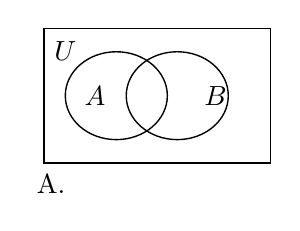
\begin{tikzpicture}[scale=0.9,line width=0.5pt]
\draw (0,0) rectangle (3.2,1.9);
\draw (1.02,0.95) ellipse (0.72 and 0.62);
\draw (1.88,0.95) ellipse (0.72 and 0.62);
\node at (0.72,0.95) {$A$};
\node at (2.42,0.95) {$B$};
\node at (0.3,1.58) {$U$};
\node[anchor=north] at (0.1,-0.03) {A.};
\end{tikzpicture}
&
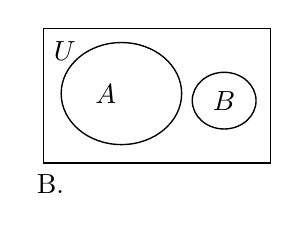
\begin{tikzpicture}[scale=0.9,line width=0.5pt]
\draw (0,0) rectangle (3.2,1.9);
\draw (1.1,0.98) ellipse (0.85 and 0.72);
\draw (2.55,0.88) ellipse (0.45 and 0.4);
\node at (0.88,0.98) {$A$};
\node at (2.55,0.88) {$B$};
\node at (0.3,1.58) {$U$};
\node[anchor=north] at (0.1,-0.03) {B.};
\end{tikzpicture}
\\[10pt]
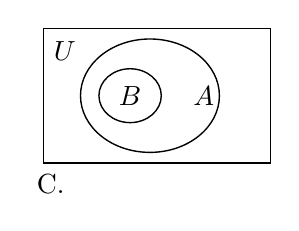
\begin{tikzpicture}[scale=0.9,line width=0.5pt]
\draw (0,0) rectangle (3.2,1.9);
\draw (1.5,0.95) ellipse (0.98 and 0.8);
\draw (1.22,0.95) ellipse (0.44 and 0.38);
\node at (1.22,0.95) {$B$};
\node at (2.26,0.95) {$A$};
\node at (0.3,1.58) {$U$};
\node[anchor=north] at (0.1,-0.03) {C.};
\end{tikzpicture}
&
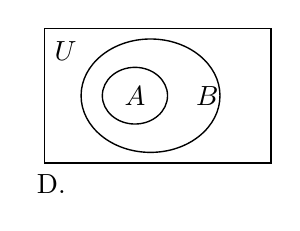
\begin{tikzpicture}[scale=0.9,line width=0.5pt]
\draw (0,0) rectangle (3.2,1.9);
\draw (1.5,0.95) ellipse (0.98 and 0.8);
\draw (1.28,0.95) ellipse (0.46 and 0.4);
\node at (1.28,0.95) {$A$};
\node at (2.3,0.95) {$B$};
\node at (0.3,1.58) {$U$};
\node[anchor=north] at (0.1,-0.03) {D.};
\end{tikzpicture}
\\
\end{tabular}
\end{center}

\ifanswer
\solbegin
\step{$\dfrac{2x-8}{x-5}\leqslant1\Rightarrow\dfrac{2x-8}{x-5}-1\leqslant0\Rightarrow\dfrac{x-3}{x-5}\leqslant0$，等价于 $\begin{cases}(x-3)(x-5)\leqslant0\\ x-5\neq0\end{cases}$，}
\step{解得 $3\leqslant x<5$，因为 $x\in\N$，所以 $A=\{3,4\}$，}
\step{解不等式 $x^2-7x+12\leqslant0$ 得 $B=\{x\mid3\leqslant x\leqslant4\}$，}
\step{集合 $A$ 中的元素 3，4 都属于集合 $B$，且 $B$ 中存在无数实数不属于 $A$，}
\step{所以 $A$ 是 $B$ 的真子集，$A$ 在 $B$ 内部．故选 $D$.}
\solend

\fi

\item 已知 $a$、$b$、$c\in\R$，则下列命题中真命题的个数是\mbox{（\quad）}

①若 $ac^2>bc^2$，则 $a>b$；②若 $\lvert a-2\rvert>\lvert b-2\rvert$，则 $(a-2)^2>(b-2)^2$；

③若 $a>b>c>0$，则 $\dfrac ab>\dfrac{a+c}{b+c}$；④若 $a>0$，$b>0$，$a+b>4$，$ab>4$，则 $a>2$，$b>2$.

\keepwithprev
A. $1$\qquad\qquad B. $2$\qquad\qquad C. $3$\qquad\qquad D. $4$

\ifanswer
\solbegin
\step{①若 $ac^2>bc^2$，则 $c^2>0$，则 $a>b$；所以①正确；}
\step{②若 $\lvert a-2\rvert>\lvert b-2\rvert$，则 $(a-2)^2>(b-2)^2$；满足不等式的基本性质，所以②正确；}
\step{③若 $a>b>c>0$，则 $\dfrac ab>\dfrac{a+c}{b+c}$；所以③正确；}
\step{④若 $a>0$，$b>0$，$a+b>4$，$ab>4$，则 $a>2$，$b>2$.}
\step{反例 $a=10$，$b=0.5$，满足条件，推不出结论，所以④不正确；}
\step{故选 $C$.}
\solend

\fi

\item 已知实数 $a<b$，关于 $x$ 的不等式 $x^2-(a+b)x+ab-1<0$ 的解集为 $(x_1,x_2)$，则实数
$a$、$b$、$x_1$、$x_2$ 从小到大的排列是\mbox{（\quad）}

\keepwithprev
A. $x_1<a<x_2<b$\qquad B. $x_1<a<b<x_2$\qquad C. $a<x_1<b<x_2$\qquad D. $a<x_1<x_2<b$

\ifanswer
\solbegin
\step{已知实数 $a<b$，关于 $x$ 的不等式 $x^2-(a+b)x+ab-1<0$ 的解集为 $(x_1,x_2)$，}
\step{因为 $x^2-(a+b)x+ab=(x-a)(x-b)$.}
\step{设函数 $g(x)=(x-a)(x-b)$，作函数 $g(x)$、$g(x)-1$ 的图象如下：}
\begin{center}
% 原图第 6 页解析插图直接裁取（原卷排于解析行右侧），已去粉色水印转灰度。
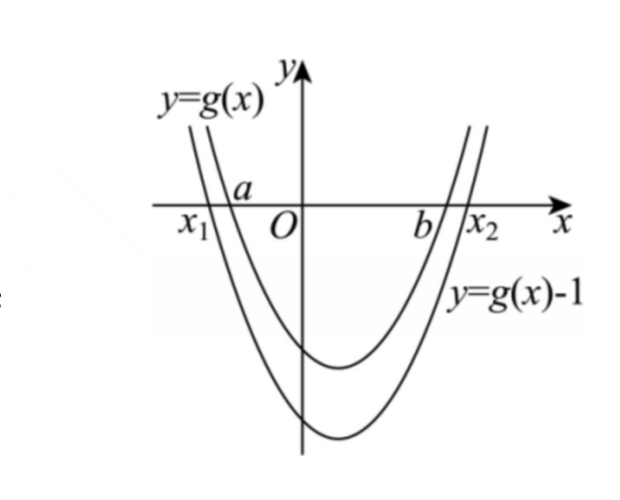
\includegraphics[width=0.20\textwidth]{figures/gao103_q16.png}
\end{center}
\step{由图像得 $x_1<a<b<x_2$．故选 $B$.}
\solend

\fi

\end{enumerate}

\bigsec{三、解答题}

\begin{enumerate}
\setcounter{enumi}{16}

\item 已知集合 $A=\{x\mid-3\leqslant x\leqslant1\}$，$B=\{x\mid a-2<x<a+2,a\in\R\}$.

（1）当 $a=1$ 时，求 $A\cap B$、$A\cup B$；

（2）若 $B\subseteq\overline A$，求 $a$ 的取值范围.

\ansspace*[8]

\ifanswer
\solbegin
\stepm{（1）}{当 $a=1$ 时，$B=\{x\mid-1<x<3\}$，又因为 $A=\{x\mid-3\leqslant x\leqslant1\}$，}
\step{所以 $A\cap B=\{x\mid-1<x\leqslant1\}$，$A\cup B=\{x\mid-3\leqslant x<3\}$；}
\stepm{（2）}{由 $A=\{x\mid-3\leqslant x\leqslant1\}$，得 $\overline A=\{x\mid x<-3\text{ 或 }x>1\}$，}
\step{若 $B\subseteq\overline A$，易得 $B=\{x\mid a-2<x<a+2,a\in\R\}\neq\varnothing$，}
\step{所以 $a+2\leqslant-3$ 或 $a-2\geqslant1$，解得 $a\leqslant-5$ 或 $a\geqslant3$，}
\step{综上所述，实数 $a$ 的取值范围是 $(-\infty,-5]\cup[3,+\infty)$.}
\solend

\fi

\item （1）解不等式 $\lvert 1-2x\rvert>x$；

（2）已知 $a$、$b$ 都是有理数，满足 $a+b\sqrt5=0$，请用反证法证明：$a=b=0$.

\ansspace*[10]

\ifanswer
\solbegin
\stepm{（1）}{①当 $x<0$ 时，左边非负，右边为负，不等式显然成立；}
\step{②当 $x\geqslant0$ 时，两边平方，$(1-2x)^2>x^2\Rightarrow3x^2-4x+1>0$}
\step{$\Rightarrow(3x-1)(x-1)>0$，解得 $x<\dfrac13$ 或 $x>1$，结合 $x\geqslant0$，}
\step{得 $0\leqslant x<\dfrac13$ 或 $x>1$；}
\step{综上，不等式解集为 $\left(-\infty,\dfrac13\right)\cup(1,+\infty)$.}
\stepm{（2）}{假设 $a,b$ 至少有一个不为零，}
\step{当 $a,b$ 中有一个为零一个不为零时，不妨设 $\begin{cases}a\neq0\\ b=0\end{cases}$，}
\step{则 $a+b\sqrt5=0\Rightarrow a=0$ 矛盾，舍；}
\step{当 $\begin{cases}a\neq0\\ b\neq0\end{cases}$ 时，$a+b\sqrt5=0\Rightarrow\sqrt5=-\dfrac ab\in\Q$，矛盾，舍，}
\step{综上假设不成立，所以 $a=b=0$.}
\solend

\fi

\item 某物流公司为了扩大业务量，计划建造一间高为 6 米，底面积为 24 平方米，且背面靠
墙的长方形形状的仓库。仓库的背面靠墙，无须建造费用，因此甲工程队给出的报价为：
仓库前面新建墙体每平方米 400 元，左右两面新建墙体每平方米 300 元，屋顶和地面以及
其他共计 28800 元.

（1）设仓库前面墙体的长为 $x$ 米 $(x>0)$，甲工程队的整体报价为 $y$ 元。若该物流公司计
划投入的改造资金不超过 60000 元，求前面墙体长 $x$ 的取值范围.

（2）在（1）的条件下，当仓库前面墙体的长度为多少时，甲工程队的整体
报价最低？

\begin{center}
% 原图第 7 页题干仓库示意图直接裁取（原卷排于题干右侧），已去粉色水印转灰度。
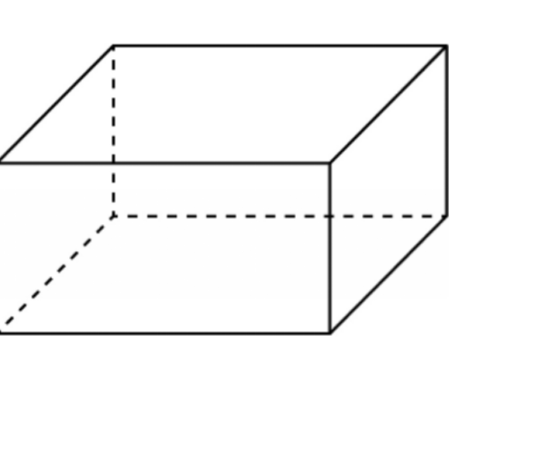
\includegraphics[width=0.17\textwidth]{figures/gao103_q19.png}
\end{center}

\ansspace*[12]

\ifanswer
\solbegin
\stepm{（1）}{甲队整体报价为 $y=400\times6x+2\times300\times6\times\dfrac{24}{x}+28800$}
\step{$=2400x+\dfrac{86400}{x}+28800$ 元，}
\step{要求 $y\leqslant60000$，即 $2400x+\dfrac{86400}{x}+28800\leqslant60000$，}
\step{化简得 $x+\dfrac{36}{x}\leqslant13$，}
\step{由于 $x>0$，则不等式化为 $x^2-13x+36\leqslant0$，}
\step{即 $(x-4)(x-9)\leqslant0$，解得 $4\leqslant x\leqslant9$，}
\step{所以前面墙体长 $x$ 的取值范围为 $[4,9]$；}
\stepm{（2）}{甲队整体报价为 $y=2400x+\dfrac{86400}{x}$}
\step{$\geqslant2\sqrt{2400x\times\dfrac{86400}{x}}+28800=57600$，}
\step{当且仅当 $2400x=\dfrac{86400}{x}$，即 $x^2=36$，}
\step{解得 $x=6$（满足 $4\leqslant x\leqslant9$）时取等号，}
\step{所以当仓库前面墙体的长度为 6 米时，甲工程队的整体报价最低，}
\step{为 57600 元.}
\solend

\fi

\item 已知函数 $f(x)=ax^2-10x+4b$.

（1）当 $a=1$，$b=4$ 时，解不等式 $f(x)\geqslant0$；

（2）若关于 $x$ 的不等式 $f(x)<0$ 的解集为 $(a,b)$，求实数 $a$、$b$ 的值；

（3）若 1 是 $f(x)$ 的零点，且 $a>0$，$b>0$，问当 $a$、$b$ 取何值时，$\dfrac1a+\dfrac1b$ 的值最小？最
小值是多少？

\ansspace*[12]

\ifanswer
\solbegin
\stepm{（1）}{将 $a=1$，$b=4$ 代入得 $f(x)=x^2-10x+16\geqslant0$，解得 $x\geqslant8$ 或 $x\leqslant2$，}
\step{所以不等式的解集为 $\{x\mid x\geqslant8\text{ 或 }x\leqslant2\}$；}
\stepm{（2）}{由题意得 $a$、$b$ 是 $ax^2-10x+4b=0$ 两根，且 $a<b$，$a>0$，}
\step{由韦达定理得 $\begin{cases}a+b=\dfrac{10}{a}\\ a\cdot b=\dfrac{4b}{a}\end{cases}$，解得 $\begin{cases}a=2\\ b=3\end{cases}$，即实数 $a$、$b$ 的值分别为 2，3；}
\stepm{（3）}{由 1 是 $f(x)$ 的零点，得 $f(1)=a-10+4b=0$，得 $a+4b=10$，}
\step{因为 $a>0$，$b>0$，}
\step{所以 $\dfrac1a+\dfrac1b=\dfrac1{10}\left(\dfrac1a+\dfrac1b\right)(a+4b)=\dfrac1{10}\left(1+4+\dfrac{4b}{a}+\dfrac ab\right)$}
\step{$\geqslant\dfrac1{10}\left(5+2\sqrt{\dfrac{4b}{a}\cdot\dfrac ab}\right)=\dfrac9{10}$，}
\step{当且仅当 $\dfrac{4b}{a}=\dfrac ab$，即 $a=\dfrac{10}3$,$b=\dfrac53$ 时取等号，}
\step{所以 $\dfrac1a+\dfrac1b$ 取最小值，且最小值为 $\dfrac9{10}$.}
\solend

\fi

\item 已知集合 $A$ 为非空集合，定义 $S=\{x\mid x=a+b,a,b\in A\}$，
$T=\{x\mid x=\lvert a-b\rvert,a,b\in A\}$.

（1）若集合 $A=\{1,3\}$，直接写出集合 $S$、$T$ (无需写计算过程)；

（2）若集合 $A=\{x_1,x_2,x_3,x_4\},x_1<x_2<x_3<x_4$，且 $T=A$，求证：$x_1+x_4=x_2+x_3$；

（3）若集合 $A=\{x\mid0\leqslant x\leqslant2026,x\in\N\}$,$S\cap T=\varnothing$．记 $\lvert A\rvert$ 为集合 $A$ 中元素的个数，求
$\lvert A\rvert$ 的最大值.

\ansspace*[16]

\ifanswer
\solbegin
\stepm{（1）}{$S=\{2,4,6\}$,$T=\{0,2\}$；}
\stepm{（2）}{集合 $T$ 中最小的元素为 0，因为 $T=A$，且 $x_1<x_2<x_3<x_4$，所以 $x_1=0$，}
\step{所以集合 $T$ 中元素为 $x_2-x_1=x_2$,$x_3-x_1=x_3$,$x_4-x_1=x_4$，}
\step{以及 $x_3-x_2$,$x_4-x_2$,$x_4-x_3$ 均属于 $A$，}
\step{因为 $x_1=0<x_3-x_2<x_4-x_2<x_4$，所以 $x_3$ 即 $x_4-x_2=x_3-x_1$，}
\step{即 $x_1+x_4=x_2+x_3$；}
\stepm{（3）}{设 $A=\{a_1,a_2,a_3,\cdots,a_k\}$ 满足题意，其中 $a_1<a_2<\cdots<a_k$，}
\step{则 $2a_1<a_1+a_2<\cdots<a_1+a_k<a_2+a_k<a_3+a_k<\cdots<a_{k-1}+a_k<2a_k$，}
\step{所以 $\lvert S\cup T\rvert\leqslant2k+1$，所以 $3k-1\leqslant2a_k+1\leqslant4053(k\in\N^*)$，}
\step{所以 $k\leqslant1351$，}
\step{实际上当 $A=\{676,677,\cdots,2026\}$ 时满足题意，}
\step{证明如下：设 $A=\{m,m+1,m+2,\cdots,2026\},m\in N$，}
\step{设 $S=\{2m,2m+1,2m+2,\cdots,4052\}$,$T=\{0,1,2,\cdots,2026-m\}$，}
\step{由题意得 $2026-m<2m$，即 $m>675\dfrac13$，}
\step{故 $m$ 的最小值是 676，于是当 $m=676$,$A$ 中的元素最多，}
\step{即 $A=\{676,677,\cdots,2026\}$ 时满足题意，}
\step{综上所述，集合 $A$ 中元素的个数的最大值是 1351.}
\solend

\fi

\end{enumerate}

\end{document}
"
% 紧凑版：xelatex "\def\iscompact{1}% 高一103_市北中学_10月月考.tex
%   —— 高一上数学“2026-2027 年市北中学高一上 10 月月考”（试卷版/答案版）
% 试卷版：xelatex 高一103_市北中学_10月月考.tex
% 答案版：xelatex "\def\isanswer{1}\input{高一103_市北中学_10月月考.tex}"
% 紧凑版：xelatex "\def\iscompact{1}\input{高一103_市北中学_10月月考.tex}"
%
% 原始材料：微信公众号“魔都数学加油站”文章，作者破晓，2026-11-01 21:56 发布；
% 连载“27学年高一103”，原文标题“27学年高一103——2026-2027年上海市市北中学高一上10月月考”；
% 原文链接：https://mp.weixin.qq.com/s/iBvF4eKw66F-kS6xLmDpBA。
% 正文为 10 张 PNG 页（第 1、3、5、6、7、10 页 2560×3620，其余 4762×6735），题目下印有【解析】，为讲评版。
% 题目、解析均据原图转录；卷面水印及公众号页脚未录入。
%
% 卷首标题：原卷印作“2026-2027 年市北中学高一上 10 月月考”（公众号标题中的“上海市”“高一上”
% 卷面标题行没有或已含，本稿照卷面），年份区间按全稿惯例排 en dash；原卷未印副标题，本稿按题目
% 内容标为“集合与常用逻辑用语、不等式”。
%
% 与原卷的排版差异：
%   ① 原文从第 3 题起，填空题编号为 3—12、选择题为 13—16、解答题为 17—21，本稿保留原题号；
%   ② 原卷每题下直接印【解析】，本稿按全稿惯例将解析置于答案版；选择题括号内未印答案，另由
%      解析末句“故选 X”给出；
%   ③ 原卷未印副标题，本稿按“知识模块”口径补出；
%   ④ 原卷填空横线按全稿惯例排为 \blankline[4.4em]；解答题按惯例加 \ansspace；选择题括号排
%      \mbox{（\quad）}；
%   ⑤ 原卷数集排斜体 $R$／$Q$（第 18 题解析 $Q$ 排粗体），按全稿惯例改 $\R$／$\Q$；
%   ⑥ 第 14 题四个文氏图选项按原图形状用 TikZ 重排；第 16、19 两题的插图裁自原图
%      （去粉色水印转灰度），第 19 题图属题干（三版都出），第 16 题图属解析（仅答案版显示）。
%
% 原卷存疑／笔误（均照录加注）：
%   第 9 题解析“故 $a+b=3b+b<0$”（$a=3b$ 代入应为 $4b$，原卷写作 $3b+b$，数值相同）；
%   第 21 题 (2) 解析“所以 $x_3$ 即 $x_4-x_2=x_3-x_1$”表述含糊（意为 $x_4-x_2$ 恰为 $T$ 中
%   介于 $x_2$ 与 $x_4$ 之间的元素 $x_3-x_1$）；
%   第 21 题 (3) 解析“所以 $|S\cup T|\leqslant2k+1$”（按上下文应为 $2a_k+1$，与后半句
%   $3k-1\leqslant2a_k+1$ 呼应），照录。
%
% 行数核对：逐题数 \step/\stepm 条数，合计 119 条（Q3：2；Q4：2；Q5：5；Q6：3；Q8：3；
% Q9：7；Q10：5；Q11：8；Q12：7；Q13：6；Q14：5；Q15：6；Q16：4；Q17：6；Q18：10；
% Q19：13；Q20：10；Q21：17），与原卷印刷行逐题相等。第 7 题只印【答案】，提 \ans{}，
% 不计入 \step 账。
%
\documentclass[a4paper,11pt]{article}
\usepackage{common}

\begin{document}

\examtitlest[3]{2026--2027 年市北中学高一上 10 月月考}{集合与常用逻辑用语、不等式}

\bigsec{一、填空题}

\begin{enumerate}
\setcounter{enumi}{2}

\item 已知实数 $x$ 满足 $\dfrac{7-x}{x+4}>0$，则 $x$ 的取值范围是\blankline[4.4em].

\ifanswer
\solbegin
\step{不等式 $\dfrac{7-x}{x+4}>0$ 可化为 $\dfrac{x-7}{x+4}<0$，等价于 $(x-7)(x+4)<0$，}
\step{解得 $-4<x<7$，所以 $x$ 的取值范围是 $\{x\mid-4<x<7\}$.}
\solend

\fi

\item 已知 $x_1$、$x_2$ 为方程 $2x^2+6x+3=0$ 的两个实数根，则 $\dfrac1{x_1}+\dfrac1{x_2}=$\blankline[4.4em].

\ifanswer
\solbegin
\step{由根与系数的关系得 $x_1+x_2=-\dfrac62=-3$，$x_1x_2=\dfrac32$，}
\step{则 $\dfrac1{x_1}+\dfrac1{x_2}=\dfrac{x_1+x_2}{x_1x_2}=-2$.}
\solend

\fi

\item 已知 $y=\lvert x-2\rvert+\lvert x-5\rvert$，$x\in\R$，则 $y$ 的最小值为\blankline[4.4em].

\ifanswer
\solbegin
\step{$y=\lvert x-2\rvert+\lvert x-5\rvert=\begin{cases}7-2x, & x<2\\ 3, & 2\leqslant x\leqslant5\\ 2x-7, & x>5\end{cases}$，}
\step{当 $x<2$ 时，$y>7-2\times2=3$；}
\step{当 $2\leqslant x\leqslant5$ 时，$y=3$；}
\step{当 $x>5$ 时，$y>2\times5-7=3$.}
\step{综上所述，$y$ 的最小值为 3.}
\solend

\fi

\item 对任意实数 $x$，等式 $ax^4+bx^3+cx^2+dx+e=x(x-2)(x^2+3)$ 恒成立，则
$b+c+d=$\blankline[4.4em].

\ifanswer
\solbegin
\step{因为 $ax^4+bx^3+cx^2+dx+e=x(x-2)(x^2+3)=(x^2-2x)(x^2+3)$}
\step{$=x^4-2x^3+3x^2-6x$，所以 $a=1$，$b=-2$，$c=3$，$d=-6$，$e=0$，}
\step{所以 $b+c+d=-2+3-6=-5$.}
\solend

\fi

\item 命题：“存在 $x\in(1,+\infty)$，使得 $ax^2+bx+c<0$”的否定形式是\blankline[4.4em].

\ifanswer
\ans{对于任意的 $x\in(1,+\infty)$，都有 $ax^2+bx+c\geqslant0$}
\fi

\item 已知集合 $A=\{x\mid mx^2-2x+1=0,x\in\R\}$ 有且仅有两个子集，则实数 $m=$\blankline[4.4em].

\ifanswer
\solbegin
\step{①当 $m=0$ 时，方程为 $-2x+1=0$，解得 $x=\dfrac12$，满足 $A=\left\{\dfrac12\right\}$ 仅有两个子集；}
\step{②当 $m\neq0$ 时，方程有两个相等实根，所以 $\Delta=4-4m=0$，解得 $m=1$；}
\step{所以实数 $m$ 的值为 0 或 1.}
\solend

\fi

\item 设 $a$、$b\in\R$，已知关于 $x$ 的不等式 $(a+b)x+(b-3a)<0$ 的解集为 $(2,+\infty)$，则不等式
$(a-2b)x+5b-a>0$ 的解集为\blankline[4.4em].

\ifanswer
\solbegin
\step{关于 $x$ 的不等式 $(a+b)x+(b-3a)<0$ 的解集为 $(2,+\infty)$，}
\step{得 $x=2$ 是 $(a+b)x+(b-3a)=0$ 的解，且 $a+b<0$，}
\step{所以 $2(a+b)+(b-3a)=0$，化简得 $a=3b$，故 $a+b=3b+b<0$，即 $b<0$，}
\step{将 $a=3b$ 代入 $(a-2b)x+5b-a>0$，}
\step{得不等式 $(a-2b)x+5b-a>0$ 即 $b(x+2)>0$，}
\step{两边都除以 $b$，得 $x+2<0$，解得 $x<-2$，}
\step{所以不等式 $(a-2b)x+5b-a>0$ 的解集为 $(-\infty,-2)$.}
\solend

\fi

\item 已知不等式 $\lvert x-a\rvert<1$ 成立的充分不必要条件是 $\dfrac12<x<\dfrac32$，则实数 $a$ 的取值范围
是\blankline[4.4em].

\ifanswer
\solbegin
\step{$\lvert x-a\rvert<1$，解得 $a-1<x<1+a$，}
\step{所以 $a-1<x<1+a$ 成立的充分不必要条件是 $\dfrac12<x<\dfrac32$，}
\step{故 $\left\{x\left|\dfrac12<x<\dfrac32\right.\right\}$ 是 $\{x\mid a-1<x<1+a\}$ 的真子集，}
\step{所以 $a-1\leqslant\dfrac12$ 且 $1+a\geqslant\dfrac32$（等号不同时成立），解得 $\dfrac12\leqslant a\leqslant\dfrac32$，}
\step{故实数 $a$ 的取值范围是 $\left[\dfrac12,\dfrac32\right]$.}
\solend

\fi

\item 定义 $A\nabla B=\left\{z\,\middle|\,z=xy+\dfrac xy,x\in A,y\in B\right\}$，设集合 $A=\{0,2\}$，$B=\{1,2\}$，$C=\{1\}$，
则集合 $(A\nabla B)\nabla C=$\blankline[4.4em].

\ifanswer
\solbegin
\step{当 $x=0$，$y=1$ 或 2 时，$z=xy+\dfrac xy=0$；}
\step{当 $x=2$，$y=1$ 时，$z=xy+\dfrac xy=4$；}
\step{当 $x=2$，$y=2$ 时，$z=xy+\dfrac xy=5$；}
\step{所以 $A\nabla B=\{0,4,5\}$；}
\step{当 $x=0$，$y=1$ 时，$z=xy+\dfrac xy=0$；}
\step{当 $x=4$，$y=1$ 时，$z=xy+\dfrac xy=8$；}
\step{当 $x=5$，$y=1$ 时，$z=xy+\dfrac xy=10$；}
\step{所以 $(A\nabla B)\nabla C=\{0,8,10\}$.}
\solend

\fi

\item 集合 $M=\{66,-11,23,10,911,-1,-18,100,0,\pi\}$ 有 10 个元素，设 $M$ 的所有非空子集为
$M_i\,(i=1,2,\cdots,1023)$，每一个 $M_i$ 中所有元素乘积为 $m_i\,(i=1,2,\cdots,1023)$，则
$m_1+m_2+m_3+\cdots+m_{1023}=$\blankline[4.4em].

\ifanswer
\solbegin
\step{因为 $M$ 的所有非空子集为 $M_i\,(i=1,2,\cdots,1023)$，这 1023 个子集分成以下几种情况：}
\step{①含 0 的子集有 512 个，这些子集均满足 $m_i=0$；}
\step{②不含 0，含 $-1$ 且还含有其它元素的子集有 255 个，}
\step{③不含 0，不含 $-1$ 但含有其它元素的子集有 255 个，}
\step{④只含 $-1$ 的子集一个 $\{-1\}$，满足 $m_i=-1$；}
\step{其中②③中的集合是一一对应的，且满足 $m_i$ 对应成相反数，}
\step{故 $m_1+m_2+m_3+\cdots+m_{1023}=512\times0+255\times0-1=-1$.}
\solend

\fi

\end{enumerate}

\bigsec{二、选择题}

\begin{enumerate}
\setcounter{enumi}{12}

\item 下列说法中，正确说法的个数是\mbox{（\quad）}

①联合国安理会常任理事国能组成一个集合；

②市北中学很喜欢足球的同学能组成一个集合；

③实数 $1,0,5,\dfrac12,\dfrac32,\dfrac64,\sqrt{\dfrac14}$ 组成的集合中有 6 个元素.

\keepwithprev
A. $0$\qquad\qquad B. $1$\qquad\qquad C. $2$\qquad\qquad D. $3$.

\ifanswer
\solbegin
\step{对于①，“联合国安理会常任理事国”满足集合的定义，故①正确；}
\step{对于②，“很喜欢”不满足集合的确定性，}
\step{市北中学很喜欢足球的同学不能组成一个集合，故②错误；}
\step{对于③，$\dfrac64=\dfrac32$，$\sqrt{\dfrac14}=\dfrac12$，由集合的元素互异性，集合中共有 5 个元素，}
\step{故③错误.}
\step{所以正确说法的个数是 1 个．故选 $B$.}
\solend

\fi

\item 已知全集 $U=\R$，集合 $A=\left\{x\,\middle|\,\dfrac{2x-8}{x-5}\leqslant1,x\in\N\right\}$，集合 $B=\{x\mid x^2-7x+12\leqslant0\}$，则
正确表示集合 $A$ 与集合 $B$ 关系的文氏图是\mbox{（\quad）}

\keepwithprev
\begin{center}
% 原卷四个文氏图选项按原图形状用 TikZ 重排。
\begin{tabular}{c@{\qquad\qquad}c}
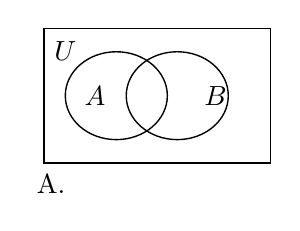
\begin{tikzpicture}[scale=0.9,line width=0.5pt]
\draw (0,0) rectangle (3.2,1.9);
\draw (1.02,0.95) ellipse (0.72 and 0.62);
\draw (1.88,0.95) ellipse (0.72 and 0.62);
\node at (0.72,0.95) {$A$};
\node at (2.42,0.95) {$B$};
\node at (0.3,1.58) {$U$};
\node[anchor=north] at (0.1,-0.03) {A.};
\end{tikzpicture}
&
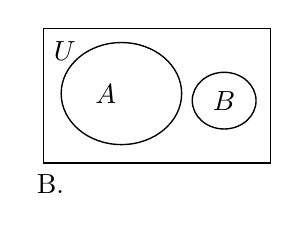
\begin{tikzpicture}[scale=0.9,line width=0.5pt]
\draw (0,0) rectangle (3.2,1.9);
\draw (1.1,0.98) ellipse (0.85 and 0.72);
\draw (2.55,0.88) ellipse (0.45 and 0.4);
\node at (0.88,0.98) {$A$};
\node at (2.55,0.88) {$B$};
\node at (0.3,1.58) {$U$};
\node[anchor=north] at (0.1,-0.03) {B.};
\end{tikzpicture}
\\[10pt]
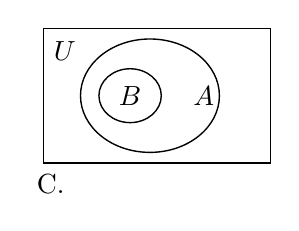
\begin{tikzpicture}[scale=0.9,line width=0.5pt]
\draw (0,0) rectangle (3.2,1.9);
\draw (1.5,0.95) ellipse (0.98 and 0.8);
\draw (1.22,0.95) ellipse (0.44 and 0.38);
\node at (1.22,0.95) {$B$};
\node at (2.26,0.95) {$A$};
\node at (0.3,1.58) {$U$};
\node[anchor=north] at (0.1,-0.03) {C.};
\end{tikzpicture}
&
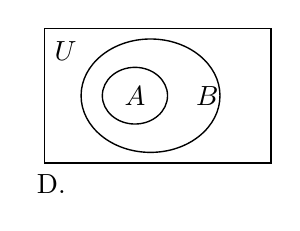
\begin{tikzpicture}[scale=0.9,line width=0.5pt]
\draw (0,0) rectangle (3.2,1.9);
\draw (1.5,0.95) ellipse (0.98 and 0.8);
\draw (1.28,0.95) ellipse (0.46 and 0.4);
\node at (1.28,0.95) {$A$};
\node at (2.3,0.95) {$B$};
\node at (0.3,1.58) {$U$};
\node[anchor=north] at (0.1,-0.03) {D.};
\end{tikzpicture}
\\
\end{tabular}
\end{center}

\ifanswer
\solbegin
\step{$\dfrac{2x-8}{x-5}\leqslant1\Rightarrow\dfrac{2x-8}{x-5}-1\leqslant0\Rightarrow\dfrac{x-3}{x-5}\leqslant0$，等价于 $\begin{cases}(x-3)(x-5)\leqslant0\\ x-5\neq0\end{cases}$，}
\step{解得 $3\leqslant x<5$，因为 $x\in\N$，所以 $A=\{3,4\}$，}
\step{解不等式 $x^2-7x+12\leqslant0$ 得 $B=\{x\mid3\leqslant x\leqslant4\}$，}
\step{集合 $A$ 中的元素 3，4 都属于集合 $B$，且 $B$ 中存在无数实数不属于 $A$，}
\step{所以 $A$ 是 $B$ 的真子集，$A$ 在 $B$ 内部．故选 $D$.}
\solend

\fi

\item 已知 $a$、$b$、$c\in\R$，则下列命题中真命题的个数是\mbox{（\quad）}

①若 $ac^2>bc^2$，则 $a>b$；②若 $\lvert a-2\rvert>\lvert b-2\rvert$，则 $(a-2)^2>(b-2)^2$；

③若 $a>b>c>0$，则 $\dfrac ab>\dfrac{a+c}{b+c}$；④若 $a>0$，$b>0$，$a+b>4$，$ab>4$，则 $a>2$，$b>2$.

\keepwithprev
A. $1$\qquad\qquad B. $2$\qquad\qquad C. $3$\qquad\qquad D. $4$

\ifanswer
\solbegin
\step{①若 $ac^2>bc^2$，则 $c^2>0$，则 $a>b$；所以①正确；}
\step{②若 $\lvert a-2\rvert>\lvert b-2\rvert$，则 $(a-2)^2>(b-2)^2$；满足不等式的基本性质，所以②正确；}
\step{③若 $a>b>c>0$，则 $\dfrac ab>\dfrac{a+c}{b+c}$；所以③正确；}
\step{④若 $a>0$，$b>0$，$a+b>4$，$ab>4$，则 $a>2$，$b>2$.}
\step{反例 $a=10$，$b=0.5$，满足条件，推不出结论，所以④不正确；}
\step{故选 $C$.}
\solend

\fi

\item 已知实数 $a<b$，关于 $x$ 的不等式 $x^2-(a+b)x+ab-1<0$ 的解集为 $(x_1,x_2)$，则实数
$a$、$b$、$x_1$、$x_2$ 从小到大的排列是\mbox{（\quad）}

\keepwithprev
A. $x_1<a<x_2<b$\qquad B. $x_1<a<b<x_2$\qquad C. $a<x_1<b<x_2$\qquad D. $a<x_1<x_2<b$

\ifanswer
\solbegin
\step{已知实数 $a<b$，关于 $x$ 的不等式 $x^2-(a+b)x+ab-1<0$ 的解集为 $(x_1,x_2)$，}
\step{因为 $x^2-(a+b)x+ab=(x-a)(x-b)$.}
\step{设函数 $g(x)=(x-a)(x-b)$，作函数 $g(x)$、$g(x)-1$ 的图象如下：}
\begin{center}
% 原图第 6 页解析插图直接裁取（原卷排于解析行右侧），已去粉色水印转灰度。
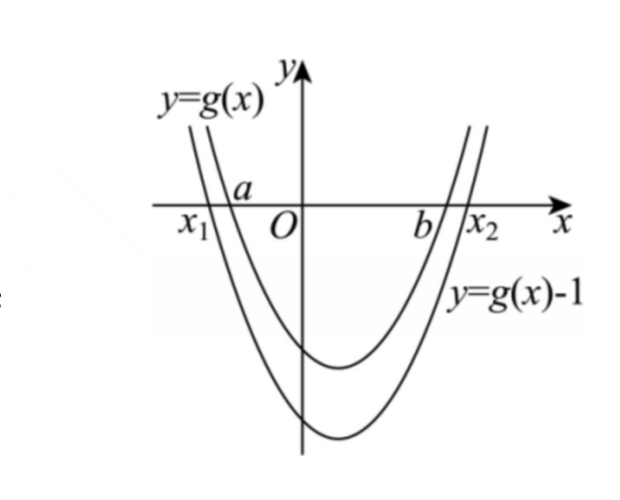
\includegraphics[width=0.20\textwidth]{figures/gao103_q16.png}
\end{center}
\step{由图像得 $x_1<a<b<x_2$．故选 $B$.}
\solend

\fi

\end{enumerate}

\bigsec{三、解答题}

\begin{enumerate}
\setcounter{enumi}{16}

\item 已知集合 $A=\{x\mid-3\leqslant x\leqslant1\}$，$B=\{x\mid a-2<x<a+2,a\in\R\}$.

（1）当 $a=1$ 时，求 $A\cap B$、$A\cup B$；

（2）若 $B\subseteq\overline A$，求 $a$ 的取值范围.

\ansspace*[8]

\ifanswer
\solbegin
\stepm{（1）}{当 $a=1$ 时，$B=\{x\mid-1<x<3\}$，又因为 $A=\{x\mid-3\leqslant x\leqslant1\}$，}
\step{所以 $A\cap B=\{x\mid-1<x\leqslant1\}$，$A\cup B=\{x\mid-3\leqslant x<3\}$；}
\stepm{（2）}{由 $A=\{x\mid-3\leqslant x\leqslant1\}$，得 $\overline A=\{x\mid x<-3\text{ 或 }x>1\}$，}
\step{若 $B\subseteq\overline A$，易得 $B=\{x\mid a-2<x<a+2,a\in\R\}\neq\varnothing$，}
\step{所以 $a+2\leqslant-3$ 或 $a-2\geqslant1$，解得 $a\leqslant-5$ 或 $a\geqslant3$，}
\step{综上所述，实数 $a$ 的取值范围是 $(-\infty,-5]\cup[3,+\infty)$.}
\solend

\fi

\item （1）解不等式 $\lvert 1-2x\rvert>x$；

（2）已知 $a$、$b$ 都是有理数，满足 $a+b\sqrt5=0$，请用反证法证明：$a=b=0$.

\ansspace*[10]

\ifanswer
\solbegin
\stepm{（1）}{①当 $x<0$ 时，左边非负，右边为负，不等式显然成立；}
\step{②当 $x\geqslant0$ 时，两边平方，$(1-2x)^2>x^2\Rightarrow3x^2-4x+1>0$}
\step{$\Rightarrow(3x-1)(x-1)>0$，解得 $x<\dfrac13$ 或 $x>1$，结合 $x\geqslant0$，}
\step{得 $0\leqslant x<\dfrac13$ 或 $x>1$；}
\step{综上，不等式解集为 $\left(-\infty,\dfrac13\right)\cup(1,+\infty)$.}
\stepm{（2）}{假设 $a,b$ 至少有一个不为零，}
\step{当 $a,b$ 中有一个为零一个不为零时，不妨设 $\begin{cases}a\neq0\\ b=0\end{cases}$，}
\step{则 $a+b\sqrt5=0\Rightarrow a=0$ 矛盾，舍；}
\step{当 $\begin{cases}a\neq0\\ b\neq0\end{cases}$ 时，$a+b\sqrt5=0\Rightarrow\sqrt5=-\dfrac ab\in\Q$，矛盾，舍，}
\step{综上假设不成立，所以 $a=b=0$.}
\solend

\fi

\item 某物流公司为了扩大业务量，计划建造一间高为 6 米，底面积为 24 平方米，且背面靠
墙的长方形形状的仓库。仓库的背面靠墙，无须建造费用，因此甲工程队给出的报价为：
仓库前面新建墙体每平方米 400 元，左右两面新建墙体每平方米 300 元，屋顶和地面以及
其他共计 28800 元.

（1）设仓库前面墙体的长为 $x$ 米 $(x>0)$，甲工程队的整体报价为 $y$ 元。若该物流公司计
划投入的改造资金不超过 60000 元，求前面墙体长 $x$ 的取值范围.

（2）在（1）的条件下，当仓库前面墙体的长度为多少时，甲工程队的整体
报价最低？

\begin{center}
% 原图第 7 页题干仓库示意图直接裁取（原卷排于题干右侧），已去粉色水印转灰度。
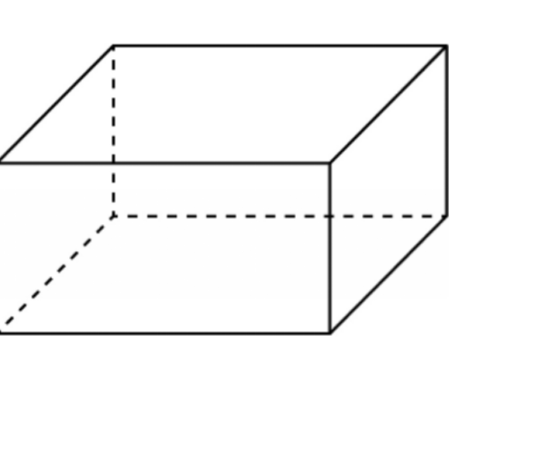
\includegraphics[width=0.17\textwidth]{figures/gao103_q19.png}
\end{center}

\ansspace*[12]

\ifanswer
\solbegin
\stepm{（1）}{甲队整体报价为 $y=400\times6x+2\times300\times6\times\dfrac{24}{x}+28800$}
\step{$=2400x+\dfrac{86400}{x}+28800$ 元，}
\step{要求 $y\leqslant60000$，即 $2400x+\dfrac{86400}{x}+28800\leqslant60000$，}
\step{化简得 $x+\dfrac{36}{x}\leqslant13$，}
\step{由于 $x>0$，则不等式化为 $x^2-13x+36\leqslant0$，}
\step{即 $(x-4)(x-9)\leqslant0$，解得 $4\leqslant x\leqslant9$，}
\step{所以前面墙体长 $x$ 的取值范围为 $[4,9]$；}
\stepm{（2）}{甲队整体报价为 $y=2400x+\dfrac{86400}{x}$}
\step{$\geqslant2\sqrt{2400x\times\dfrac{86400}{x}}+28800=57600$，}
\step{当且仅当 $2400x=\dfrac{86400}{x}$，即 $x^2=36$，}
\step{解得 $x=6$（满足 $4\leqslant x\leqslant9$）时取等号，}
\step{所以当仓库前面墙体的长度为 6 米时，甲工程队的整体报价最低，}
\step{为 57600 元.}
\solend

\fi

\item 已知函数 $f(x)=ax^2-10x+4b$.

（1）当 $a=1$，$b=4$ 时，解不等式 $f(x)\geqslant0$；

（2）若关于 $x$ 的不等式 $f(x)<0$ 的解集为 $(a,b)$，求实数 $a$、$b$ 的值；

（3）若 1 是 $f(x)$ 的零点，且 $a>0$，$b>0$，问当 $a$、$b$ 取何值时，$\dfrac1a+\dfrac1b$ 的值最小？最
小值是多少？

\ansspace*[12]

\ifanswer
\solbegin
\stepm{（1）}{将 $a=1$，$b=4$ 代入得 $f(x)=x^2-10x+16\geqslant0$，解得 $x\geqslant8$ 或 $x\leqslant2$，}
\step{所以不等式的解集为 $\{x\mid x\geqslant8\text{ 或 }x\leqslant2\}$；}
\stepm{（2）}{由题意得 $a$、$b$ 是 $ax^2-10x+4b=0$ 两根，且 $a<b$，$a>0$，}
\step{由韦达定理得 $\begin{cases}a+b=\dfrac{10}{a}\\ a\cdot b=\dfrac{4b}{a}\end{cases}$，解得 $\begin{cases}a=2\\ b=3\end{cases}$，即实数 $a$、$b$ 的值分别为 2，3；}
\stepm{（3）}{由 1 是 $f(x)$ 的零点，得 $f(1)=a-10+4b=0$，得 $a+4b=10$，}
\step{因为 $a>0$，$b>0$，}
\step{所以 $\dfrac1a+\dfrac1b=\dfrac1{10}\left(\dfrac1a+\dfrac1b\right)(a+4b)=\dfrac1{10}\left(1+4+\dfrac{4b}{a}+\dfrac ab\right)$}
\step{$\geqslant\dfrac1{10}\left(5+2\sqrt{\dfrac{4b}{a}\cdot\dfrac ab}\right)=\dfrac9{10}$，}
\step{当且仅当 $\dfrac{4b}{a}=\dfrac ab$，即 $a=\dfrac{10}3$,$b=\dfrac53$ 时取等号，}
\step{所以 $\dfrac1a+\dfrac1b$ 取最小值，且最小值为 $\dfrac9{10}$.}
\solend

\fi

\item 已知集合 $A$ 为非空集合，定义 $S=\{x\mid x=a+b,a,b\in A\}$，
$T=\{x\mid x=\lvert a-b\rvert,a,b\in A\}$.

（1）若集合 $A=\{1,3\}$，直接写出集合 $S$、$T$ (无需写计算过程)；

（2）若集合 $A=\{x_1,x_2,x_3,x_4\},x_1<x_2<x_3<x_4$，且 $T=A$，求证：$x_1+x_4=x_2+x_3$；

（3）若集合 $A=\{x\mid0\leqslant x\leqslant2026,x\in\N\}$,$S\cap T=\varnothing$．记 $\lvert A\rvert$ 为集合 $A$ 中元素的个数，求
$\lvert A\rvert$ 的最大值.

\ansspace*[16]

\ifanswer
\solbegin
\stepm{（1）}{$S=\{2,4,6\}$,$T=\{0,2\}$；}
\stepm{（2）}{集合 $T$ 中最小的元素为 0，因为 $T=A$，且 $x_1<x_2<x_3<x_4$，所以 $x_1=0$，}
\step{所以集合 $T$ 中元素为 $x_2-x_1=x_2$,$x_3-x_1=x_3$,$x_4-x_1=x_4$，}
\step{以及 $x_3-x_2$,$x_4-x_2$,$x_4-x_3$ 均属于 $A$，}
\step{因为 $x_1=0<x_3-x_2<x_4-x_2<x_4$，所以 $x_3$ 即 $x_4-x_2=x_3-x_1$，}
\step{即 $x_1+x_4=x_2+x_3$；}
\stepm{（3）}{设 $A=\{a_1,a_2,a_3,\cdots,a_k\}$ 满足题意，其中 $a_1<a_2<\cdots<a_k$，}
\step{则 $2a_1<a_1+a_2<\cdots<a_1+a_k<a_2+a_k<a_3+a_k<\cdots<a_{k-1}+a_k<2a_k$，}
\step{所以 $\lvert S\cup T\rvert\leqslant2k+1$，所以 $3k-1\leqslant2a_k+1\leqslant4053(k\in\N^*)$，}
\step{所以 $k\leqslant1351$，}
\step{实际上当 $A=\{676,677,\cdots,2026\}$ 时满足题意，}
\step{证明如下：设 $A=\{m,m+1,m+2,\cdots,2026\},m\in N$，}
\step{设 $S=\{2m,2m+1,2m+2,\cdots,4052\}$,$T=\{0,1,2,\cdots,2026-m\}$，}
\step{由题意得 $2026-m<2m$，即 $m>675\dfrac13$，}
\step{故 $m$ 的最小值是 676，于是当 $m=676$,$A$ 中的元素最多，}
\step{即 $A=\{676,677,\cdots,2026\}$ 时满足题意，}
\step{综上所述，集合 $A$ 中元素的个数的最大值是 1351.}
\solend

\fi

\end{enumerate}

\end{document}
"
%
% 原始材料：微信公众号“魔都数学加油站”文章，作者破晓，2026-11-01 21:56 发布；
% 连载“27学年高一103”，原文标题“27学年高一103——2026-2027年上海市市北中学高一上10月月考”；
% 原文链接：https://mp.weixin.qq.com/s/iBvF4eKw66F-kS6xLmDpBA。
% 正文为 10 张 PNG 页（第 1、3、5、6、7、10 页 2560×3620，其余 4762×6735），题目下印有【解析】，为讲评版。
% 题目、解析均据原图转录；卷面水印及公众号页脚未录入。
%
% 卷首标题：原卷印作“2026-2027 年市北中学高一上 10 月月考”（公众号标题中的“上海市”“高一上”
% 卷面标题行没有或已含，本稿照卷面），年份区间按全稿惯例排 en dash；原卷未印副标题，本稿按题目
% 内容标为“集合与常用逻辑用语、不等式”。
%
% 与原卷的排版差异：
%   ① 原文从第 3 题起，填空题编号为 3—12、选择题为 13—16、解答题为 17—21，本稿保留原题号；
%   ② 原卷每题下直接印【解析】，本稿按全稿惯例将解析置于答案版；选择题括号内未印答案，另由
%      解析末句“故选 X”给出；
%   ③ 原卷未印副标题，本稿按“知识模块”口径补出；
%   ④ 原卷填空横线按全稿惯例排为 \blankline[4.4em]；解答题按惯例加 \ansspace；选择题括号排
%      \mbox{（\quad）}；
%   ⑤ 原卷数集排斜体 $R$／$Q$（第 18 题解析 $Q$ 排粗体），按全稿惯例改 $\R$／$\Q$；
%   ⑥ 第 14 题四个文氏图选项按原图形状用 TikZ 重排；第 16、19 两题的插图裁自原图
%      （去粉色水印转灰度），第 19 题图属题干（三版都出），第 16 题图属解析（仅答案版显示）。
%
% 原卷存疑／笔误（均照录加注）：
%   第 9 题解析“故 $a+b=3b+b<0$”（$a=3b$ 代入应为 $4b$，原卷写作 $3b+b$，数值相同）；
%   第 21 题 (2) 解析“所以 $x_3$ 即 $x_4-x_2=x_3-x_1$”表述含糊（意为 $x_4-x_2$ 恰为 $T$ 中
%   介于 $x_2$ 与 $x_4$ 之间的元素 $x_3-x_1$）；
%   第 21 题 (3) 解析“所以 $|S\cup T|\leqslant2k+1$”（按上下文应为 $2a_k+1$，与后半句
%   $3k-1\leqslant2a_k+1$ 呼应），照录。
%
% 行数核对：逐题数 \step/\stepm 条数，合计 119 条（Q3：2；Q4：2；Q5：5；Q6：3；Q8：3；
% Q9：7；Q10：5；Q11：8；Q12：7；Q13：6；Q14：5；Q15：6；Q16：4；Q17：6；Q18：10；
% Q19：13；Q20：10；Q21：17），与原卷印刷行逐题相等。第 7 题只印【答案】，提 \ans{}，
% 不计入 \step 账。
%
\documentclass[a4paper,11pt]{article}
\usepackage{common}

\begin{document}

\examtitlest[3]{2026--2027 年市北中学高一上 10 月月考}{集合与常用逻辑用语、不等式}

\bigsec{一、填空题}

\begin{enumerate}
\setcounter{enumi}{2}

\item 已知实数 $x$ 满足 $\dfrac{7-x}{x+4}>0$，则 $x$ 的取值范围是\blankline[4.4em].

\ifanswer
\solbegin
\step{不等式 $\dfrac{7-x}{x+4}>0$ 可化为 $\dfrac{x-7}{x+4}<0$，等价于 $(x-7)(x+4)<0$，}
\step{解得 $-4<x<7$，所以 $x$ 的取值范围是 $\{x\mid-4<x<7\}$.}
\solend

\fi

\item 已知 $x_1$、$x_2$ 为方程 $2x^2+6x+3=0$ 的两个实数根，则 $\dfrac1{x_1}+\dfrac1{x_2}=$\blankline[4.4em].

\ifanswer
\solbegin
\step{由根与系数的关系得 $x_1+x_2=-\dfrac62=-3$，$x_1x_2=\dfrac32$，}
\step{则 $\dfrac1{x_1}+\dfrac1{x_2}=\dfrac{x_1+x_2}{x_1x_2}=-2$.}
\solend

\fi

\item 已知 $y=\lvert x-2\rvert+\lvert x-5\rvert$，$x\in\R$，则 $y$ 的最小值为\blankline[4.4em].

\ifanswer
\solbegin
\step{$y=\lvert x-2\rvert+\lvert x-5\rvert=\begin{cases}7-2x, & x<2\\ 3, & 2\leqslant x\leqslant5\\ 2x-7, & x>5\end{cases}$，}
\step{当 $x<2$ 时，$y>7-2\times2=3$；}
\step{当 $2\leqslant x\leqslant5$ 时，$y=3$；}
\step{当 $x>5$ 时，$y>2\times5-7=3$.}
\step{综上所述，$y$ 的最小值为 3.}
\solend

\fi

\item 对任意实数 $x$，等式 $ax^4+bx^3+cx^2+dx+e=x(x-2)(x^2+3)$ 恒成立，则
$b+c+d=$\blankline[4.4em].

\ifanswer
\solbegin
\step{因为 $ax^4+bx^3+cx^2+dx+e=x(x-2)(x^2+3)=(x^2-2x)(x^2+3)$}
\step{$=x^4-2x^3+3x^2-6x$，所以 $a=1$，$b=-2$，$c=3$，$d=-6$，$e=0$，}
\step{所以 $b+c+d=-2+3-6=-5$.}
\solend

\fi

\item 命题：“存在 $x\in(1,+\infty)$，使得 $ax^2+bx+c<0$”的否定形式是\blankline[4.4em].

\ifanswer
\ans{对于任意的 $x\in(1,+\infty)$，都有 $ax^2+bx+c\geqslant0$}
\fi

\item 已知集合 $A=\{x\mid mx^2-2x+1=0,x\in\R\}$ 有且仅有两个子集，则实数 $m=$\blankline[4.4em].

\ifanswer
\solbegin
\step{①当 $m=0$ 时，方程为 $-2x+1=0$，解得 $x=\dfrac12$，满足 $A=\left\{\dfrac12\right\}$ 仅有两个子集；}
\step{②当 $m\neq0$ 时，方程有两个相等实根，所以 $\Delta=4-4m=0$，解得 $m=1$；}
\step{所以实数 $m$ 的值为 0 或 1.}
\solend

\fi

\item 设 $a$、$b\in\R$，已知关于 $x$ 的不等式 $(a+b)x+(b-3a)<0$ 的解集为 $(2,+\infty)$，则不等式
$(a-2b)x+5b-a>0$ 的解集为\blankline[4.4em].

\ifanswer
\solbegin
\step{关于 $x$ 的不等式 $(a+b)x+(b-3a)<0$ 的解集为 $(2,+\infty)$，}
\step{得 $x=2$ 是 $(a+b)x+(b-3a)=0$ 的解，且 $a+b<0$，}
\step{所以 $2(a+b)+(b-3a)=0$，化简得 $a=3b$，故 $a+b=3b+b<0$，即 $b<0$，}
\step{将 $a=3b$ 代入 $(a-2b)x+5b-a>0$，}
\step{得不等式 $(a-2b)x+5b-a>0$ 即 $b(x+2)>0$，}
\step{两边都除以 $b$，得 $x+2<0$，解得 $x<-2$，}
\step{所以不等式 $(a-2b)x+5b-a>0$ 的解集为 $(-\infty,-2)$.}
\solend

\fi

\item 已知不等式 $\lvert x-a\rvert<1$ 成立的充分不必要条件是 $\dfrac12<x<\dfrac32$，则实数 $a$ 的取值范围
是\blankline[4.4em].

\ifanswer
\solbegin
\step{$\lvert x-a\rvert<1$，解得 $a-1<x<1+a$，}
\step{所以 $a-1<x<1+a$ 成立的充分不必要条件是 $\dfrac12<x<\dfrac32$，}
\step{故 $\left\{x\left|\dfrac12<x<\dfrac32\right.\right\}$ 是 $\{x\mid a-1<x<1+a\}$ 的真子集，}
\step{所以 $a-1\leqslant\dfrac12$ 且 $1+a\geqslant\dfrac32$（等号不同时成立），解得 $\dfrac12\leqslant a\leqslant\dfrac32$，}
\step{故实数 $a$ 的取值范围是 $\left[\dfrac12,\dfrac32\right]$.}
\solend

\fi

\item 定义 $A\nabla B=\left\{z\,\middle|\,z=xy+\dfrac xy,x\in A,y\in B\right\}$，设集合 $A=\{0,2\}$，$B=\{1,2\}$，$C=\{1\}$，
则集合 $(A\nabla B)\nabla C=$\blankline[4.4em].

\ifanswer
\solbegin
\step{当 $x=0$，$y=1$ 或 2 时，$z=xy+\dfrac xy=0$；}
\step{当 $x=2$，$y=1$ 时，$z=xy+\dfrac xy=4$；}
\step{当 $x=2$，$y=2$ 时，$z=xy+\dfrac xy=5$；}
\step{所以 $A\nabla B=\{0,4,5\}$；}
\step{当 $x=0$，$y=1$ 时，$z=xy+\dfrac xy=0$；}
\step{当 $x=4$，$y=1$ 时，$z=xy+\dfrac xy=8$；}
\step{当 $x=5$，$y=1$ 时，$z=xy+\dfrac xy=10$；}
\step{所以 $(A\nabla B)\nabla C=\{0,8,10\}$.}
\solend

\fi

\item 集合 $M=\{66,-11,23,10,911,-1,-18,100,0,\pi\}$ 有 10 个元素，设 $M$ 的所有非空子集为
$M_i\,(i=1,2,\cdots,1023)$，每一个 $M_i$ 中所有元素乘积为 $m_i\,(i=1,2,\cdots,1023)$，则
$m_1+m_2+m_3+\cdots+m_{1023}=$\blankline[4.4em].

\ifanswer
\solbegin
\step{因为 $M$ 的所有非空子集为 $M_i\,(i=1,2,\cdots,1023)$，这 1023 个子集分成以下几种情况：}
\step{①含 0 的子集有 512 个，这些子集均满足 $m_i=0$；}
\step{②不含 0，含 $-1$ 且还含有其它元素的子集有 255 个，}
\step{③不含 0，不含 $-1$ 但含有其它元素的子集有 255 个，}
\step{④只含 $-1$ 的子集一个 $\{-1\}$，满足 $m_i=-1$；}
\step{其中②③中的集合是一一对应的，且满足 $m_i$ 对应成相反数，}
\step{故 $m_1+m_2+m_3+\cdots+m_{1023}=512\times0+255\times0-1=-1$.}
\solend

\fi

\end{enumerate}

\bigsec{二、选择题}

\begin{enumerate}
\setcounter{enumi}{12}

\item 下列说法中，正确说法的个数是\mbox{（\quad）}

①联合国安理会常任理事国能组成一个集合；

②市北中学很喜欢足球的同学能组成一个集合；

③实数 $1,0,5,\dfrac12,\dfrac32,\dfrac64,\sqrt{\dfrac14}$ 组成的集合中有 6 个元素.

\keepwithprev
A. $0$\qquad\qquad B. $1$\qquad\qquad C. $2$\qquad\qquad D. $3$.

\ifanswer
\solbegin
\step{对于①，“联合国安理会常任理事国”满足集合的定义，故①正确；}
\step{对于②，“很喜欢”不满足集合的确定性，}
\step{市北中学很喜欢足球的同学不能组成一个集合，故②错误；}
\step{对于③，$\dfrac64=\dfrac32$，$\sqrt{\dfrac14}=\dfrac12$，由集合的元素互异性，集合中共有 5 个元素，}
\step{故③错误.}
\step{所以正确说法的个数是 1 个．故选 $B$.}
\solend

\fi

\item 已知全集 $U=\R$，集合 $A=\left\{x\,\middle|\,\dfrac{2x-8}{x-5}\leqslant1,x\in\N\right\}$，集合 $B=\{x\mid x^2-7x+12\leqslant0\}$，则
正确表示集合 $A$ 与集合 $B$ 关系的文氏图是\mbox{（\quad）}

\keepwithprev
\begin{center}
% 原卷四个文氏图选项按原图形状用 TikZ 重排。
\begin{tabular}{c@{\qquad\qquad}c}
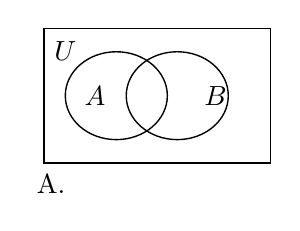
\begin{tikzpicture}[scale=0.9,line width=0.5pt]
\draw (0,0) rectangle (3.2,1.9);
\draw (1.02,0.95) ellipse (0.72 and 0.62);
\draw (1.88,0.95) ellipse (0.72 and 0.62);
\node at (0.72,0.95) {$A$};
\node at (2.42,0.95) {$B$};
\node at (0.3,1.58) {$U$};
\node[anchor=north] at (0.1,-0.03) {A.};
\end{tikzpicture}
&
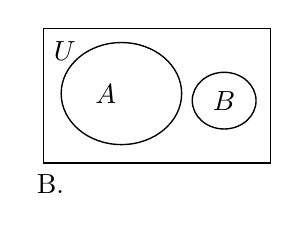
\begin{tikzpicture}[scale=0.9,line width=0.5pt]
\draw (0,0) rectangle (3.2,1.9);
\draw (1.1,0.98) ellipse (0.85 and 0.72);
\draw (2.55,0.88) ellipse (0.45 and 0.4);
\node at (0.88,0.98) {$A$};
\node at (2.55,0.88) {$B$};
\node at (0.3,1.58) {$U$};
\node[anchor=north] at (0.1,-0.03) {B.};
\end{tikzpicture}
\\[10pt]
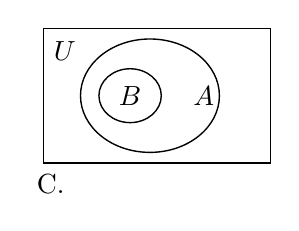
\begin{tikzpicture}[scale=0.9,line width=0.5pt]
\draw (0,0) rectangle (3.2,1.9);
\draw (1.5,0.95) ellipse (0.98 and 0.8);
\draw (1.22,0.95) ellipse (0.44 and 0.38);
\node at (1.22,0.95) {$B$};
\node at (2.26,0.95) {$A$};
\node at (0.3,1.58) {$U$};
\node[anchor=north] at (0.1,-0.03) {C.};
\end{tikzpicture}
&
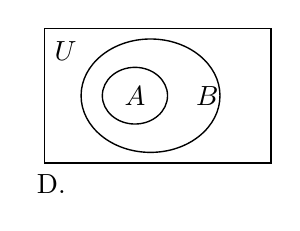
\begin{tikzpicture}[scale=0.9,line width=0.5pt]
\draw (0,0) rectangle (3.2,1.9);
\draw (1.5,0.95) ellipse (0.98 and 0.8);
\draw (1.28,0.95) ellipse (0.46 and 0.4);
\node at (1.28,0.95) {$A$};
\node at (2.3,0.95) {$B$};
\node at (0.3,1.58) {$U$};
\node[anchor=north] at (0.1,-0.03) {D.};
\end{tikzpicture}
\\
\end{tabular}
\end{center}

\ifanswer
\solbegin
\step{$\dfrac{2x-8}{x-5}\leqslant1\Rightarrow\dfrac{2x-8}{x-5}-1\leqslant0\Rightarrow\dfrac{x-3}{x-5}\leqslant0$，等价于 $\begin{cases}(x-3)(x-5)\leqslant0\\ x-5\neq0\end{cases}$，}
\step{解得 $3\leqslant x<5$，因为 $x\in\N$，所以 $A=\{3,4\}$，}
\step{解不等式 $x^2-7x+12\leqslant0$ 得 $B=\{x\mid3\leqslant x\leqslant4\}$，}
\step{集合 $A$ 中的元素 3，4 都属于集合 $B$，且 $B$ 中存在无数实数不属于 $A$，}
\step{所以 $A$ 是 $B$ 的真子集，$A$ 在 $B$ 内部．故选 $D$.}
\solend

\fi

\item 已知 $a$、$b$、$c\in\R$，则下列命题中真命题的个数是\mbox{（\quad）}

①若 $ac^2>bc^2$，则 $a>b$；②若 $\lvert a-2\rvert>\lvert b-2\rvert$，则 $(a-2)^2>(b-2)^2$；

③若 $a>b>c>0$，则 $\dfrac ab>\dfrac{a+c}{b+c}$；④若 $a>0$，$b>0$，$a+b>4$，$ab>4$，则 $a>2$，$b>2$.

\keepwithprev
A. $1$\qquad\qquad B. $2$\qquad\qquad C. $3$\qquad\qquad D. $4$

\ifanswer
\solbegin
\step{①若 $ac^2>bc^2$，则 $c^2>0$，则 $a>b$；所以①正确；}
\step{②若 $\lvert a-2\rvert>\lvert b-2\rvert$，则 $(a-2)^2>(b-2)^2$；满足不等式的基本性质，所以②正确；}
\step{③若 $a>b>c>0$，则 $\dfrac ab>\dfrac{a+c}{b+c}$；所以③正确；}
\step{④若 $a>0$，$b>0$，$a+b>4$，$ab>4$，则 $a>2$，$b>2$.}
\step{反例 $a=10$，$b=0.5$，满足条件，推不出结论，所以④不正确；}
\step{故选 $C$.}
\solend

\fi

\item 已知实数 $a<b$，关于 $x$ 的不等式 $x^2-(a+b)x+ab-1<0$ 的解集为 $(x_1,x_2)$，则实数
$a$、$b$、$x_1$、$x_2$ 从小到大的排列是\mbox{（\quad）}

\keepwithprev
A. $x_1<a<x_2<b$\qquad B. $x_1<a<b<x_2$\qquad C. $a<x_1<b<x_2$\qquad D. $a<x_1<x_2<b$

\ifanswer
\solbegin
\step{已知实数 $a<b$，关于 $x$ 的不等式 $x^2-(a+b)x+ab-1<0$ 的解集为 $(x_1,x_2)$，}
\step{因为 $x^2-(a+b)x+ab=(x-a)(x-b)$.}
\step{设函数 $g(x)=(x-a)(x-b)$，作函数 $g(x)$、$g(x)-1$ 的图象如下：}
\begin{center}
% 原图第 6 页解析插图直接裁取（原卷排于解析行右侧），已去粉色水印转灰度。
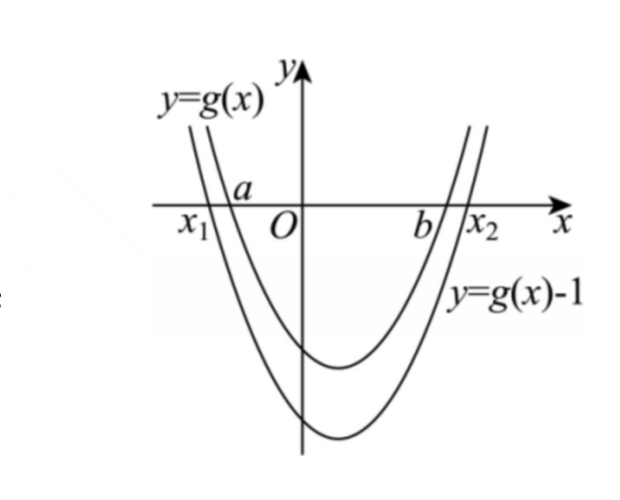
\includegraphics[width=0.20\textwidth]{figures/gao103_q16.png}
\end{center}
\step{由图像得 $x_1<a<b<x_2$．故选 $B$.}
\solend

\fi

\end{enumerate}

\bigsec{三、解答题}

\begin{enumerate}
\setcounter{enumi}{16}

\item 已知集合 $A=\{x\mid-3\leqslant x\leqslant1\}$，$B=\{x\mid a-2<x<a+2,a\in\R\}$.

（1）当 $a=1$ 时，求 $A\cap B$、$A\cup B$；

（2）若 $B\subseteq\overline A$，求 $a$ 的取值范围.

\ansspace*[8]

\ifanswer
\solbegin
\stepm{（1）}{当 $a=1$ 时，$B=\{x\mid-1<x<3\}$，又因为 $A=\{x\mid-3\leqslant x\leqslant1\}$，}
\step{所以 $A\cap B=\{x\mid-1<x\leqslant1\}$，$A\cup B=\{x\mid-3\leqslant x<3\}$；}
\stepm{（2）}{由 $A=\{x\mid-3\leqslant x\leqslant1\}$，得 $\overline A=\{x\mid x<-3\text{ 或 }x>1\}$，}
\step{若 $B\subseteq\overline A$，易得 $B=\{x\mid a-2<x<a+2,a\in\R\}\neq\varnothing$，}
\step{所以 $a+2\leqslant-3$ 或 $a-2\geqslant1$，解得 $a\leqslant-5$ 或 $a\geqslant3$，}
\step{综上所述，实数 $a$ 的取值范围是 $(-\infty,-5]\cup[3,+\infty)$.}
\solend

\fi

\item （1）解不等式 $\lvert 1-2x\rvert>x$；

（2）已知 $a$、$b$ 都是有理数，满足 $a+b\sqrt5=0$，请用反证法证明：$a=b=0$.

\ansspace*[10]

\ifanswer
\solbegin
\stepm{（1）}{①当 $x<0$ 时，左边非负，右边为负，不等式显然成立；}
\step{②当 $x\geqslant0$ 时，两边平方，$(1-2x)^2>x^2\Rightarrow3x^2-4x+1>0$}
\step{$\Rightarrow(3x-1)(x-1)>0$，解得 $x<\dfrac13$ 或 $x>1$，结合 $x\geqslant0$，}
\step{得 $0\leqslant x<\dfrac13$ 或 $x>1$；}
\step{综上，不等式解集为 $\left(-\infty,\dfrac13\right)\cup(1,+\infty)$.}
\stepm{（2）}{假设 $a,b$ 至少有一个不为零，}
\step{当 $a,b$ 中有一个为零一个不为零时，不妨设 $\begin{cases}a\neq0\\ b=0\end{cases}$，}
\step{则 $a+b\sqrt5=0\Rightarrow a=0$ 矛盾，舍；}
\step{当 $\begin{cases}a\neq0\\ b\neq0\end{cases}$ 时，$a+b\sqrt5=0\Rightarrow\sqrt5=-\dfrac ab\in\Q$，矛盾，舍，}
\step{综上假设不成立，所以 $a=b=0$.}
\solend

\fi

\item 某物流公司为了扩大业务量，计划建造一间高为 6 米，底面积为 24 平方米，且背面靠
墙的长方形形状的仓库。仓库的背面靠墙，无须建造费用，因此甲工程队给出的报价为：
仓库前面新建墙体每平方米 400 元，左右两面新建墙体每平方米 300 元，屋顶和地面以及
其他共计 28800 元.

（1）设仓库前面墙体的长为 $x$ 米 $(x>0)$，甲工程队的整体报价为 $y$ 元。若该物流公司计
划投入的改造资金不超过 60000 元，求前面墙体长 $x$ 的取值范围.

（2）在（1）的条件下，当仓库前面墙体的长度为多少时，甲工程队的整体
报价最低？

\begin{center}
% 原图第 7 页题干仓库示意图直接裁取（原卷排于题干右侧），已去粉色水印转灰度。
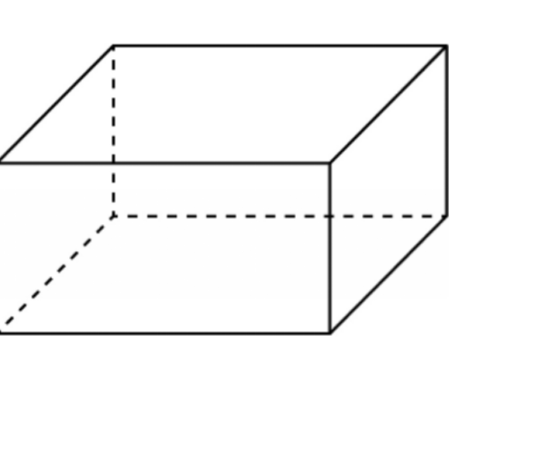
\includegraphics[width=0.17\textwidth]{figures/gao103_q19.png}
\end{center}

\ansspace*[12]

\ifanswer
\solbegin
\stepm{（1）}{甲队整体报价为 $y=400\times6x+2\times300\times6\times\dfrac{24}{x}+28800$}
\step{$=2400x+\dfrac{86400}{x}+28800$ 元，}
\step{要求 $y\leqslant60000$，即 $2400x+\dfrac{86400}{x}+28800\leqslant60000$，}
\step{化简得 $x+\dfrac{36}{x}\leqslant13$，}
\step{由于 $x>0$，则不等式化为 $x^2-13x+36\leqslant0$，}
\step{即 $(x-4)(x-9)\leqslant0$，解得 $4\leqslant x\leqslant9$，}
\step{所以前面墙体长 $x$ 的取值范围为 $[4,9]$；}
\stepm{（2）}{甲队整体报价为 $y=2400x+\dfrac{86400}{x}$}
\step{$\geqslant2\sqrt{2400x\times\dfrac{86400}{x}}+28800=57600$，}
\step{当且仅当 $2400x=\dfrac{86400}{x}$，即 $x^2=36$，}
\step{解得 $x=6$（满足 $4\leqslant x\leqslant9$）时取等号，}
\step{所以当仓库前面墙体的长度为 6 米时，甲工程队的整体报价最低，}
\step{为 57600 元.}
\solend

\fi

\item 已知函数 $f(x)=ax^2-10x+4b$.

（1）当 $a=1$，$b=4$ 时，解不等式 $f(x)\geqslant0$；

（2）若关于 $x$ 的不等式 $f(x)<0$ 的解集为 $(a,b)$，求实数 $a$、$b$ 的值；

（3）若 1 是 $f(x)$ 的零点，且 $a>0$，$b>0$，问当 $a$、$b$ 取何值时，$\dfrac1a+\dfrac1b$ 的值最小？最
小值是多少？

\ansspace*[12]

\ifanswer
\solbegin
\stepm{（1）}{将 $a=1$，$b=4$ 代入得 $f(x)=x^2-10x+16\geqslant0$，解得 $x\geqslant8$ 或 $x\leqslant2$，}
\step{所以不等式的解集为 $\{x\mid x\geqslant8\text{ 或 }x\leqslant2\}$；}
\stepm{（2）}{由题意得 $a$、$b$ 是 $ax^2-10x+4b=0$ 两根，且 $a<b$，$a>0$，}
\step{由韦达定理得 $\begin{cases}a+b=\dfrac{10}{a}\\ a\cdot b=\dfrac{4b}{a}\end{cases}$，解得 $\begin{cases}a=2\\ b=3\end{cases}$，即实数 $a$、$b$ 的值分别为 2，3；}
\stepm{（3）}{由 1 是 $f(x)$ 的零点，得 $f(1)=a-10+4b=0$，得 $a+4b=10$，}
\step{因为 $a>0$，$b>0$，}
\step{所以 $\dfrac1a+\dfrac1b=\dfrac1{10}\left(\dfrac1a+\dfrac1b\right)(a+4b)=\dfrac1{10}\left(1+4+\dfrac{4b}{a}+\dfrac ab\right)$}
\step{$\geqslant\dfrac1{10}\left(5+2\sqrt{\dfrac{4b}{a}\cdot\dfrac ab}\right)=\dfrac9{10}$，}
\step{当且仅当 $\dfrac{4b}{a}=\dfrac ab$，即 $a=\dfrac{10}3$,$b=\dfrac53$ 时取等号，}
\step{所以 $\dfrac1a+\dfrac1b$ 取最小值，且最小值为 $\dfrac9{10}$.}
\solend

\fi

\item 已知集合 $A$ 为非空集合，定义 $S=\{x\mid x=a+b,a,b\in A\}$，
$T=\{x\mid x=\lvert a-b\rvert,a,b\in A\}$.

（1）若集合 $A=\{1,3\}$，直接写出集合 $S$、$T$ (无需写计算过程)；

（2）若集合 $A=\{x_1,x_2,x_3,x_4\},x_1<x_2<x_3<x_4$，且 $T=A$，求证：$x_1+x_4=x_2+x_3$；

（3）若集合 $A=\{x\mid0\leqslant x\leqslant2026,x\in\N\}$,$S\cap T=\varnothing$．记 $\lvert A\rvert$ 为集合 $A$ 中元素的个数，求
$\lvert A\rvert$ 的最大值.

\ansspace*[16]

\ifanswer
\solbegin
\stepm{（1）}{$S=\{2,4,6\}$,$T=\{0,2\}$；}
\stepm{（2）}{集合 $T$ 中最小的元素为 0，因为 $T=A$，且 $x_1<x_2<x_3<x_4$，所以 $x_1=0$，}
\step{所以集合 $T$ 中元素为 $x_2-x_1=x_2$,$x_3-x_1=x_3$,$x_4-x_1=x_4$，}
\step{以及 $x_3-x_2$,$x_4-x_2$,$x_4-x_3$ 均属于 $A$，}
\step{因为 $x_1=0<x_3-x_2<x_4-x_2<x_4$，所以 $x_3$ 即 $x_4-x_2=x_3-x_1$，}
\step{即 $x_1+x_4=x_2+x_3$；}
\stepm{（3）}{设 $A=\{a_1,a_2,a_3,\cdots,a_k\}$ 满足题意，其中 $a_1<a_2<\cdots<a_k$，}
\step{则 $2a_1<a_1+a_2<\cdots<a_1+a_k<a_2+a_k<a_3+a_k<\cdots<a_{k-1}+a_k<2a_k$，}
\step{所以 $\lvert S\cup T\rvert\leqslant2k+1$，所以 $3k-1\leqslant2a_k+1\leqslant4053(k\in\N^*)$，}
\step{所以 $k\leqslant1351$，}
\step{实际上当 $A=\{676,677,\cdots,2026\}$ 时满足题意，}
\step{证明如下：设 $A=\{m,m+1,m+2,\cdots,2026\},m\in N$，}
\step{设 $S=\{2m,2m+1,2m+2,\cdots,4052\}$,$T=\{0,1,2,\cdots,2026-m\}$，}
\step{由题意得 $2026-m<2m$，即 $m>675\dfrac13$，}
\step{故 $m$ 的最小值是 676，于是当 $m=676$,$A$ 中的元素最多，}
\step{即 $A=\{676,677,\cdots,2026\}$ 时满足题意，}
\step{综上所述，集合 $A$ 中元素的个数的最大值是 1351.}
\solend

\fi

\end{enumerate}

\end{document}
"
% 紧凑版：xelatex "\def\iscompact{1}% 高一103_市北中学_10月月考.tex
%   —— 高一上数学“2026-2027 年市北中学高一上 10 月月考”（试卷版/答案版）
% 试卷版：xelatex 高一103_市北中学_10月月考.tex
% 答案版：xelatex "\def\isanswer{1}% 高一103_市北中学_10月月考.tex
%   —— 高一上数学“2026-2027 年市北中学高一上 10 月月考”（试卷版/答案版）
% 试卷版：xelatex 高一103_市北中学_10月月考.tex
% 答案版：xelatex "\def\isanswer{1}\input{高一103_市北中学_10月月考.tex}"
% 紧凑版：xelatex "\def\iscompact{1}\input{高一103_市北中学_10月月考.tex}"
%
% 原始材料：微信公众号“魔都数学加油站”文章，作者破晓，2026-11-01 21:56 发布；
% 连载“27学年高一103”，原文标题“27学年高一103——2026-2027年上海市市北中学高一上10月月考”；
% 原文链接：https://mp.weixin.qq.com/s/iBvF4eKw66F-kS6xLmDpBA。
% 正文为 10 张 PNG 页（第 1、3、5、6、7、10 页 2560×3620，其余 4762×6735），题目下印有【解析】，为讲评版。
% 题目、解析均据原图转录；卷面水印及公众号页脚未录入。
%
% 卷首标题：原卷印作“2026-2027 年市北中学高一上 10 月月考”（公众号标题中的“上海市”“高一上”
% 卷面标题行没有或已含，本稿照卷面），年份区间按全稿惯例排 en dash；原卷未印副标题，本稿按题目
% 内容标为“集合与常用逻辑用语、不等式”。
%
% 与原卷的排版差异：
%   ① 原文从第 3 题起，填空题编号为 3—12、选择题为 13—16、解答题为 17—21，本稿保留原题号；
%   ② 原卷每题下直接印【解析】，本稿按全稿惯例将解析置于答案版；选择题括号内未印答案，另由
%      解析末句“故选 X”给出；
%   ③ 原卷未印副标题，本稿按“知识模块”口径补出；
%   ④ 原卷填空横线按全稿惯例排为 \blankline[4.4em]；解答题按惯例加 \ansspace；选择题括号排
%      \mbox{（\quad）}；
%   ⑤ 原卷数集排斜体 $R$／$Q$（第 18 题解析 $Q$ 排粗体），按全稿惯例改 $\R$／$\Q$；
%   ⑥ 第 14 题四个文氏图选项按原图形状用 TikZ 重排；第 16、19 两题的插图裁自原图
%      （去粉色水印转灰度），第 19 题图属题干（三版都出），第 16 题图属解析（仅答案版显示）。
%
% 原卷存疑／笔误（均照录加注）：
%   第 9 题解析“故 $a+b=3b+b<0$”（$a=3b$ 代入应为 $4b$，原卷写作 $3b+b$，数值相同）；
%   第 21 题 (2) 解析“所以 $x_3$ 即 $x_4-x_2=x_3-x_1$”表述含糊（意为 $x_4-x_2$ 恰为 $T$ 中
%   介于 $x_2$ 与 $x_4$ 之间的元素 $x_3-x_1$）；
%   第 21 题 (3) 解析“所以 $|S\cup T|\leqslant2k+1$”（按上下文应为 $2a_k+1$，与后半句
%   $3k-1\leqslant2a_k+1$ 呼应），照录。
%
% 行数核对：逐题数 \step/\stepm 条数，合计 119 条（Q3：2；Q4：2；Q5：5；Q6：3；Q8：3；
% Q9：7；Q10：5；Q11：8；Q12：7；Q13：6；Q14：5；Q15：6；Q16：4；Q17：6；Q18：10；
% Q19：13；Q20：10；Q21：17），与原卷印刷行逐题相等。第 7 题只印【答案】，提 \ans{}，
% 不计入 \step 账。
%
\documentclass[a4paper,11pt]{article}
\usepackage{common}

\begin{document}

\examtitlest[3]{2026--2027 年市北中学高一上 10 月月考}{集合与常用逻辑用语、不等式}

\bigsec{一、填空题}

\begin{enumerate}
\setcounter{enumi}{2}

\item 已知实数 $x$ 满足 $\dfrac{7-x}{x+4}>0$，则 $x$ 的取值范围是\blankline[4.4em].

\ifanswer
\solbegin
\step{不等式 $\dfrac{7-x}{x+4}>0$ 可化为 $\dfrac{x-7}{x+4}<0$，等价于 $(x-7)(x+4)<0$，}
\step{解得 $-4<x<7$，所以 $x$ 的取值范围是 $\{x\mid-4<x<7\}$.}
\solend

\fi

\item 已知 $x_1$、$x_2$ 为方程 $2x^2+6x+3=0$ 的两个实数根，则 $\dfrac1{x_1}+\dfrac1{x_2}=$\blankline[4.4em].

\ifanswer
\solbegin
\step{由根与系数的关系得 $x_1+x_2=-\dfrac62=-3$，$x_1x_2=\dfrac32$，}
\step{则 $\dfrac1{x_1}+\dfrac1{x_2}=\dfrac{x_1+x_2}{x_1x_2}=-2$.}
\solend

\fi

\item 已知 $y=\lvert x-2\rvert+\lvert x-5\rvert$，$x\in\R$，则 $y$ 的最小值为\blankline[4.4em].

\ifanswer
\solbegin
\step{$y=\lvert x-2\rvert+\lvert x-5\rvert=\begin{cases}7-2x, & x<2\\ 3, & 2\leqslant x\leqslant5\\ 2x-7, & x>5\end{cases}$，}
\step{当 $x<2$ 时，$y>7-2\times2=3$；}
\step{当 $2\leqslant x\leqslant5$ 时，$y=3$；}
\step{当 $x>5$ 时，$y>2\times5-7=3$.}
\step{综上所述，$y$ 的最小值为 3.}
\solend

\fi

\item 对任意实数 $x$，等式 $ax^4+bx^3+cx^2+dx+e=x(x-2)(x^2+3)$ 恒成立，则
$b+c+d=$\blankline[4.4em].

\ifanswer
\solbegin
\step{因为 $ax^4+bx^3+cx^2+dx+e=x(x-2)(x^2+3)=(x^2-2x)(x^2+3)$}
\step{$=x^4-2x^3+3x^2-6x$，所以 $a=1$，$b=-2$，$c=3$，$d=-6$，$e=0$，}
\step{所以 $b+c+d=-2+3-6=-5$.}
\solend

\fi

\item 命题：“存在 $x\in(1,+\infty)$，使得 $ax^2+bx+c<0$”的否定形式是\blankline[4.4em].

\ifanswer
\ans{对于任意的 $x\in(1,+\infty)$，都有 $ax^2+bx+c\geqslant0$}
\fi

\item 已知集合 $A=\{x\mid mx^2-2x+1=0,x\in\R\}$ 有且仅有两个子集，则实数 $m=$\blankline[4.4em].

\ifanswer
\solbegin
\step{①当 $m=0$ 时，方程为 $-2x+1=0$，解得 $x=\dfrac12$，满足 $A=\left\{\dfrac12\right\}$ 仅有两个子集；}
\step{②当 $m\neq0$ 时，方程有两个相等实根，所以 $\Delta=4-4m=0$，解得 $m=1$；}
\step{所以实数 $m$ 的值为 0 或 1.}
\solend

\fi

\item 设 $a$、$b\in\R$，已知关于 $x$ 的不等式 $(a+b)x+(b-3a)<0$ 的解集为 $(2,+\infty)$，则不等式
$(a-2b)x+5b-a>0$ 的解集为\blankline[4.4em].

\ifanswer
\solbegin
\step{关于 $x$ 的不等式 $(a+b)x+(b-3a)<0$ 的解集为 $(2,+\infty)$，}
\step{得 $x=2$ 是 $(a+b)x+(b-3a)=0$ 的解，且 $a+b<0$，}
\step{所以 $2(a+b)+(b-3a)=0$，化简得 $a=3b$，故 $a+b=3b+b<0$，即 $b<0$，}
\step{将 $a=3b$ 代入 $(a-2b)x+5b-a>0$，}
\step{得不等式 $(a-2b)x+5b-a>0$ 即 $b(x+2)>0$，}
\step{两边都除以 $b$，得 $x+2<0$，解得 $x<-2$，}
\step{所以不等式 $(a-2b)x+5b-a>0$ 的解集为 $(-\infty,-2)$.}
\solend

\fi

\item 已知不等式 $\lvert x-a\rvert<1$ 成立的充分不必要条件是 $\dfrac12<x<\dfrac32$，则实数 $a$ 的取值范围
是\blankline[4.4em].

\ifanswer
\solbegin
\step{$\lvert x-a\rvert<1$，解得 $a-1<x<1+a$，}
\step{所以 $a-1<x<1+a$ 成立的充分不必要条件是 $\dfrac12<x<\dfrac32$，}
\step{故 $\left\{x\left|\dfrac12<x<\dfrac32\right.\right\}$ 是 $\{x\mid a-1<x<1+a\}$ 的真子集，}
\step{所以 $a-1\leqslant\dfrac12$ 且 $1+a\geqslant\dfrac32$（等号不同时成立），解得 $\dfrac12\leqslant a\leqslant\dfrac32$，}
\step{故实数 $a$ 的取值范围是 $\left[\dfrac12,\dfrac32\right]$.}
\solend

\fi

\item 定义 $A\nabla B=\left\{z\,\middle|\,z=xy+\dfrac xy,x\in A,y\in B\right\}$，设集合 $A=\{0,2\}$，$B=\{1,2\}$，$C=\{1\}$，
则集合 $(A\nabla B)\nabla C=$\blankline[4.4em].

\ifanswer
\solbegin
\step{当 $x=0$，$y=1$ 或 2 时，$z=xy+\dfrac xy=0$；}
\step{当 $x=2$，$y=1$ 时，$z=xy+\dfrac xy=4$；}
\step{当 $x=2$，$y=2$ 时，$z=xy+\dfrac xy=5$；}
\step{所以 $A\nabla B=\{0,4,5\}$；}
\step{当 $x=0$，$y=1$ 时，$z=xy+\dfrac xy=0$；}
\step{当 $x=4$，$y=1$ 时，$z=xy+\dfrac xy=8$；}
\step{当 $x=5$，$y=1$ 时，$z=xy+\dfrac xy=10$；}
\step{所以 $(A\nabla B)\nabla C=\{0,8,10\}$.}
\solend

\fi

\item 集合 $M=\{66,-11,23,10,911,-1,-18,100,0,\pi\}$ 有 10 个元素，设 $M$ 的所有非空子集为
$M_i\,(i=1,2,\cdots,1023)$，每一个 $M_i$ 中所有元素乘积为 $m_i\,(i=1,2,\cdots,1023)$，则
$m_1+m_2+m_3+\cdots+m_{1023}=$\blankline[4.4em].

\ifanswer
\solbegin
\step{因为 $M$ 的所有非空子集为 $M_i\,(i=1,2,\cdots,1023)$，这 1023 个子集分成以下几种情况：}
\step{①含 0 的子集有 512 个，这些子集均满足 $m_i=0$；}
\step{②不含 0，含 $-1$ 且还含有其它元素的子集有 255 个，}
\step{③不含 0，不含 $-1$ 但含有其它元素的子集有 255 个，}
\step{④只含 $-1$ 的子集一个 $\{-1\}$，满足 $m_i=-1$；}
\step{其中②③中的集合是一一对应的，且满足 $m_i$ 对应成相反数，}
\step{故 $m_1+m_2+m_3+\cdots+m_{1023}=512\times0+255\times0-1=-1$.}
\solend

\fi

\end{enumerate}

\bigsec{二、选择题}

\begin{enumerate}
\setcounter{enumi}{12}

\item 下列说法中，正确说法的个数是\mbox{（\quad）}

①联合国安理会常任理事国能组成一个集合；

②市北中学很喜欢足球的同学能组成一个集合；

③实数 $1,0,5,\dfrac12,\dfrac32,\dfrac64,\sqrt{\dfrac14}$ 组成的集合中有 6 个元素.

\keepwithprev
A. $0$\qquad\qquad B. $1$\qquad\qquad C. $2$\qquad\qquad D. $3$.

\ifanswer
\solbegin
\step{对于①，“联合国安理会常任理事国”满足集合的定义，故①正确；}
\step{对于②，“很喜欢”不满足集合的确定性，}
\step{市北中学很喜欢足球的同学不能组成一个集合，故②错误；}
\step{对于③，$\dfrac64=\dfrac32$，$\sqrt{\dfrac14}=\dfrac12$，由集合的元素互异性，集合中共有 5 个元素，}
\step{故③错误.}
\step{所以正确说法的个数是 1 个．故选 $B$.}
\solend

\fi

\item 已知全集 $U=\R$，集合 $A=\left\{x\,\middle|\,\dfrac{2x-8}{x-5}\leqslant1,x\in\N\right\}$，集合 $B=\{x\mid x^2-7x+12\leqslant0\}$，则
正确表示集合 $A$ 与集合 $B$ 关系的文氏图是\mbox{（\quad）}

\keepwithprev
\begin{center}
% 原卷四个文氏图选项按原图形状用 TikZ 重排。
\begin{tabular}{c@{\qquad\qquad}c}
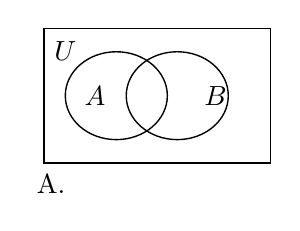
\begin{tikzpicture}[scale=0.9,line width=0.5pt]
\draw (0,0) rectangle (3.2,1.9);
\draw (1.02,0.95) ellipse (0.72 and 0.62);
\draw (1.88,0.95) ellipse (0.72 and 0.62);
\node at (0.72,0.95) {$A$};
\node at (2.42,0.95) {$B$};
\node at (0.3,1.58) {$U$};
\node[anchor=north] at (0.1,-0.03) {A.};
\end{tikzpicture}
&
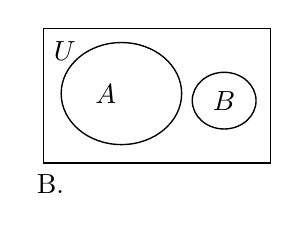
\begin{tikzpicture}[scale=0.9,line width=0.5pt]
\draw (0,0) rectangle (3.2,1.9);
\draw (1.1,0.98) ellipse (0.85 and 0.72);
\draw (2.55,0.88) ellipse (0.45 and 0.4);
\node at (0.88,0.98) {$A$};
\node at (2.55,0.88) {$B$};
\node at (0.3,1.58) {$U$};
\node[anchor=north] at (0.1,-0.03) {B.};
\end{tikzpicture}
\\[10pt]
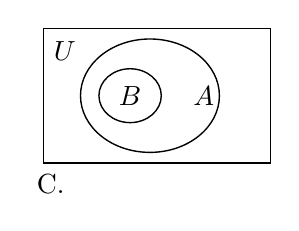
\begin{tikzpicture}[scale=0.9,line width=0.5pt]
\draw (0,0) rectangle (3.2,1.9);
\draw (1.5,0.95) ellipse (0.98 and 0.8);
\draw (1.22,0.95) ellipse (0.44 and 0.38);
\node at (1.22,0.95) {$B$};
\node at (2.26,0.95) {$A$};
\node at (0.3,1.58) {$U$};
\node[anchor=north] at (0.1,-0.03) {C.};
\end{tikzpicture}
&
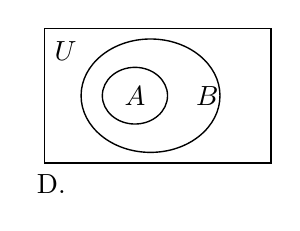
\begin{tikzpicture}[scale=0.9,line width=0.5pt]
\draw (0,0) rectangle (3.2,1.9);
\draw (1.5,0.95) ellipse (0.98 and 0.8);
\draw (1.28,0.95) ellipse (0.46 and 0.4);
\node at (1.28,0.95) {$A$};
\node at (2.3,0.95) {$B$};
\node at (0.3,1.58) {$U$};
\node[anchor=north] at (0.1,-0.03) {D.};
\end{tikzpicture}
\\
\end{tabular}
\end{center}

\ifanswer
\solbegin
\step{$\dfrac{2x-8}{x-5}\leqslant1\Rightarrow\dfrac{2x-8}{x-5}-1\leqslant0\Rightarrow\dfrac{x-3}{x-5}\leqslant0$，等价于 $\begin{cases}(x-3)(x-5)\leqslant0\\ x-5\neq0\end{cases}$，}
\step{解得 $3\leqslant x<5$，因为 $x\in\N$，所以 $A=\{3,4\}$，}
\step{解不等式 $x^2-7x+12\leqslant0$ 得 $B=\{x\mid3\leqslant x\leqslant4\}$，}
\step{集合 $A$ 中的元素 3，4 都属于集合 $B$，且 $B$ 中存在无数实数不属于 $A$，}
\step{所以 $A$ 是 $B$ 的真子集，$A$ 在 $B$ 内部．故选 $D$.}
\solend

\fi

\item 已知 $a$、$b$、$c\in\R$，则下列命题中真命题的个数是\mbox{（\quad）}

①若 $ac^2>bc^2$，则 $a>b$；②若 $\lvert a-2\rvert>\lvert b-2\rvert$，则 $(a-2)^2>(b-2)^2$；

③若 $a>b>c>0$，则 $\dfrac ab>\dfrac{a+c}{b+c}$；④若 $a>0$，$b>0$，$a+b>4$，$ab>4$，则 $a>2$，$b>2$.

\keepwithprev
A. $1$\qquad\qquad B. $2$\qquad\qquad C. $3$\qquad\qquad D. $4$

\ifanswer
\solbegin
\step{①若 $ac^2>bc^2$，则 $c^2>0$，则 $a>b$；所以①正确；}
\step{②若 $\lvert a-2\rvert>\lvert b-2\rvert$，则 $(a-2)^2>(b-2)^2$；满足不等式的基本性质，所以②正确；}
\step{③若 $a>b>c>0$，则 $\dfrac ab>\dfrac{a+c}{b+c}$；所以③正确；}
\step{④若 $a>0$，$b>0$，$a+b>4$，$ab>4$，则 $a>2$，$b>2$.}
\step{反例 $a=10$，$b=0.5$，满足条件，推不出结论，所以④不正确；}
\step{故选 $C$.}
\solend

\fi

\item 已知实数 $a<b$，关于 $x$ 的不等式 $x^2-(a+b)x+ab-1<0$ 的解集为 $(x_1,x_2)$，则实数
$a$、$b$、$x_1$、$x_2$ 从小到大的排列是\mbox{（\quad）}

\keepwithprev
A. $x_1<a<x_2<b$\qquad B. $x_1<a<b<x_2$\qquad C. $a<x_1<b<x_2$\qquad D. $a<x_1<x_2<b$

\ifanswer
\solbegin
\step{已知实数 $a<b$，关于 $x$ 的不等式 $x^2-(a+b)x+ab-1<0$ 的解集为 $(x_1,x_2)$，}
\step{因为 $x^2-(a+b)x+ab=(x-a)(x-b)$.}
\step{设函数 $g(x)=(x-a)(x-b)$，作函数 $g(x)$、$g(x)-1$ 的图象如下：}
\begin{center}
% 原图第 6 页解析插图直接裁取（原卷排于解析行右侧），已去粉色水印转灰度。
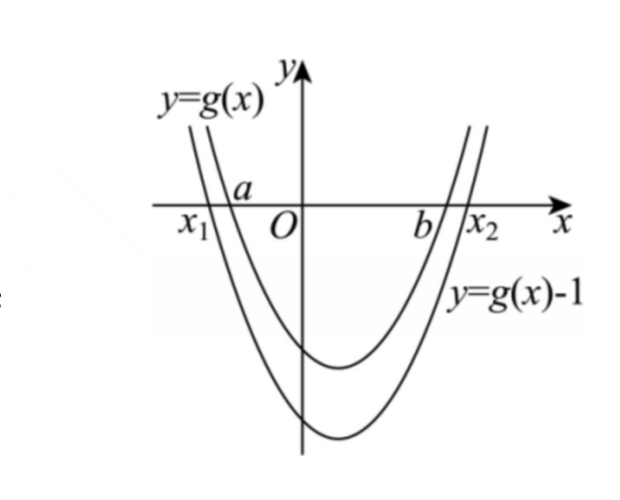
\includegraphics[width=0.20\textwidth]{figures/gao103_q16.png}
\end{center}
\step{由图像得 $x_1<a<b<x_2$．故选 $B$.}
\solend

\fi

\end{enumerate}

\bigsec{三、解答题}

\begin{enumerate}
\setcounter{enumi}{16}

\item 已知集合 $A=\{x\mid-3\leqslant x\leqslant1\}$，$B=\{x\mid a-2<x<a+2,a\in\R\}$.

（1）当 $a=1$ 时，求 $A\cap B$、$A\cup B$；

（2）若 $B\subseteq\overline A$，求 $a$ 的取值范围.

\ansspace*[8]

\ifanswer
\solbegin
\stepm{（1）}{当 $a=1$ 时，$B=\{x\mid-1<x<3\}$，又因为 $A=\{x\mid-3\leqslant x\leqslant1\}$，}
\step{所以 $A\cap B=\{x\mid-1<x\leqslant1\}$，$A\cup B=\{x\mid-3\leqslant x<3\}$；}
\stepm{（2）}{由 $A=\{x\mid-3\leqslant x\leqslant1\}$，得 $\overline A=\{x\mid x<-3\text{ 或 }x>1\}$，}
\step{若 $B\subseteq\overline A$，易得 $B=\{x\mid a-2<x<a+2,a\in\R\}\neq\varnothing$，}
\step{所以 $a+2\leqslant-3$ 或 $a-2\geqslant1$，解得 $a\leqslant-5$ 或 $a\geqslant3$，}
\step{综上所述，实数 $a$ 的取值范围是 $(-\infty,-5]\cup[3,+\infty)$.}
\solend

\fi

\item （1）解不等式 $\lvert 1-2x\rvert>x$；

（2）已知 $a$、$b$ 都是有理数，满足 $a+b\sqrt5=0$，请用反证法证明：$a=b=0$.

\ansspace*[10]

\ifanswer
\solbegin
\stepm{（1）}{①当 $x<0$ 时，左边非负，右边为负，不等式显然成立；}
\step{②当 $x\geqslant0$ 时，两边平方，$(1-2x)^2>x^2\Rightarrow3x^2-4x+1>0$}
\step{$\Rightarrow(3x-1)(x-1)>0$，解得 $x<\dfrac13$ 或 $x>1$，结合 $x\geqslant0$，}
\step{得 $0\leqslant x<\dfrac13$ 或 $x>1$；}
\step{综上，不等式解集为 $\left(-\infty,\dfrac13\right)\cup(1,+\infty)$.}
\stepm{（2）}{假设 $a,b$ 至少有一个不为零，}
\step{当 $a,b$ 中有一个为零一个不为零时，不妨设 $\begin{cases}a\neq0\\ b=0\end{cases}$，}
\step{则 $a+b\sqrt5=0\Rightarrow a=0$ 矛盾，舍；}
\step{当 $\begin{cases}a\neq0\\ b\neq0\end{cases}$ 时，$a+b\sqrt5=0\Rightarrow\sqrt5=-\dfrac ab\in\Q$，矛盾，舍，}
\step{综上假设不成立，所以 $a=b=0$.}
\solend

\fi

\item 某物流公司为了扩大业务量，计划建造一间高为 6 米，底面积为 24 平方米，且背面靠
墙的长方形形状的仓库。仓库的背面靠墙，无须建造费用，因此甲工程队给出的报价为：
仓库前面新建墙体每平方米 400 元，左右两面新建墙体每平方米 300 元，屋顶和地面以及
其他共计 28800 元.

（1）设仓库前面墙体的长为 $x$ 米 $(x>0)$，甲工程队的整体报价为 $y$ 元。若该物流公司计
划投入的改造资金不超过 60000 元，求前面墙体长 $x$ 的取值范围.

（2）在（1）的条件下，当仓库前面墙体的长度为多少时，甲工程队的整体
报价最低？

\begin{center}
% 原图第 7 页题干仓库示意图直接裁取（原卷排于题干右侧），已去粉色水印转灰度。
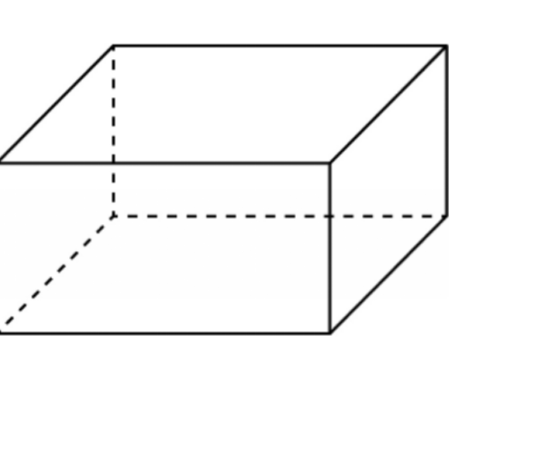
\includegraphics[width=0.17\textwidth]{figures/gao103_q19.png}
\end{center}

\ansspace*[12]

\ifanswer
\solbegin
\stepm{（1）}{甲队整体报价为 $y=400\times6x+2\times300\times6\times\dfrac{24}{x}+28800$}
\step{$=2400x+\dfrac{86400}{x}+28800$ 元，}
\step{要求 $y\leqslant60000$，即 $2400x+\dfrac{86400}{x}+28800\leqslant60000$，}
\step{化简得 $x+\dfrac{36}{x}\leqslant13$，}
\step{由于 $x>0$，则不等式化为 $x^2-13x+36\leqslant0$，}
\step{即 $(x-4)(x-9)\leqslant0$，解得 $4\leqslant x\leqslant9$，}
\step{所以前面墙体长 $x$ 的取值范围为 $[4,9]$；}
\stepm{（2）}{甲队整体报价为 $y=2400x+\dfrac{86400}{x}$}
\step{$\geqslant2\sqrt{2400x\times\dfrac{86400}{x}}+28800=57600$，}
\step{当且仅当 $2400x=\dfrac{86400}{x}$，即 $x^2=36$，}
\step{解得 $x=6$（满足 $4\leqslant x\leqslant9$）时取等号，}
\step{所以当仓库前面墙体的长度为 6 米时，甲工程队的整体报价最低，}
\step{为 57600 元.}
\solend

\fi

\item 已知函数 $f(x)=ax^2-10x+4b$.

（1）当 $a=1$，$b=4$ 时，解不等式 $f(x)\geqslant0$；

（2）若关于 $x$ 的不等式 $f(x)<0$ 的解集为 $(a,b)$，求实数 $a$、$b$ 的值；

（3）若 1 是 $f(x)$ 的零点，且 $a>0$，$b>0$，问当 $a$、$b$ 取何值时，$\dfrac1a+\dfrac1b$ 的值最小？最
小值是多少？

\ansspace*[12]

\ifanswer
\solbegin
\stepm{（1）}{将 $a=1$，$b=4$ 代入得 $f(x)=x^2-10x+16\geqslant0$，解得 $x\geqslant8$ 或 $x\leqslant2$，}
\step{所以不等式的解集为 $\{x\mid x\geqslant8\text{ 或 }x\leqslant2\}$；}
\stepm{（2）}{由题意得 $a$、$b$ 是 $ax^2-10x+4b=0$ 两根，且 $a<b$，$a>0$，}
\step{由韦达定理得 $\begin{cases}a+b=\dfrac{10}{a}\\ a\cdot b=\dfrac{4b}{a}\end{cases}$，解得 $\begin{cases}a=2\\ b=3\end{cases}$，即实数 $a$、$b$ 的值分别为 2，3；}
\stepm{（3）}{由 1 是 $f(x)$ 的零点，得 $f(1)=a-10+4b=0$，得 $a+4b=10$，}
\step{因为 $a>0$，$b>0$，}
\step{所以 $\dfrac1a+\dfrac1b=\dfrac1{10}\left(\dfrac1a+\dfrac1b\right)(a+4b)=\dfrac1{10}\left(1+4+\dfrac{4b}{a}+\dfrac ab\right)$}
\step{$\geqslant\dfrac1{10}\left(5+2\sqrt{\dfrac{4b}{a}\cdot\dfrac ab}\right)=\dfrac9{10}$，}
\step{当且仅当 $\dfrac{4b}{a}=\dfrac ab$，即 $a=\dfrac{10}3$,$b=\dfrac53$ 时取等号，}
\step{所以 $\dfrac1a+\dfrac1b$ 取最小值，且最小值为 $\dfrac9{10}$.}
\solend

\fi

\item 已知集合 $A$ 为非空集合，定义 $S=\{x\mid x=a+b,a,b\in A\}$，
$T=\{x\mid x=\lvert a-b\rvert,a,b\in A\}$.

（1）若集合 $A=\{1,3\}$，直接写出集合 $S$、$T$ (无需写计算过程)；

（2）若集合 $A=\{x_1,x_2,x_3,x_4\},x_1<x_2<x_3<x_4$，且 $T=A$，求证：$x_1+x_4=x_2+x_3$；

（3）若集合 $A=\{x\mid0\leqslant x\leqslant2026,x\in\N\}$,$S\cap T=\varnothing$．记 $\lvert A\rvert$ 为集合 $A$ 中元素的个数，求
$\lvert A\rvert$ 的最大值.

\ansspace*[16]

\ifanswer
\solbegin
\stepm{（1）}{$S=\{2,4,6\}$,$T=\{0,2\}$；}
\stepm{（2）}{集合 $T$ 中最小的元素为 0，因为 $T=A$，且 $x_1<x_2<x_3<x_4$，所以 $x_1=0$，}
\step{所以集合 $T$ 中元素为 $x_2-x_1=x_2$,$x_3-x_1=x_3$,$x_4-x_1=x_4$，}
\step{以及 $x_3-x_2$,$x_4-x_2$,$x_4-x_3$ 均属于 $A$，}
\step{因为 $x_1=0<x_3-x_2<x_4-x_2<x_4$，所以 $x_3$ 即 $x_4-x_2=x_3-x_1$，}
\step{即 $x_1+x_4=x_2+x_3$；}
\stepm{（3）}{设 $A=\{a_1,a_2,a_3,\cdots,a_k\}$ 满足题意，其中 $a_1<a_2<\cdots<a_k$，}
\step{则 $2a_1<a_1+a_2<\cdots<a_1+a_k<a_2+a_k<a_3+a_k<\cdots<a_{k-1}+a_k<2a_k$，}
\step{所以 $\lvert S\cup T\rvert\leqslant2k+1$，所以 $3k-1\leqslant2a_k+1\leqslant4053(k\in\N^*)$，}
\step{所以 $k\leqslant1351$，}
\step{实际上当 $A=\{676,677,\cdots,2026\}$ 时满足题意，}
\step{证明如下：设 $A=\{m,m+1,m+2,\cdots,2026\},m\in N$，}
\step{设 $S=\{2m,2m+1,2m+2,\cdots,4052\}$,$T=\{0,1,2,\cdots,2026-m\}$，}
\step{由题意得 $2026-m<2m$，即 $m>675\dfrac13$，}
\step{故 $m$ 的最小值是 676，于是当 $m=676$,$A$ 中的元素最多，}
\step{即 $A=\{676,677,\cdots,2026\}$ 时满足题意，}
\step{综上所述，集合 $A$ 中元素的个数的最大值是 1351.}
\solend

\fi

\end{enumerate}

\end{document}
"
% 紧凑版：xelatex "\def\iscompact{1}% 高一103_市北中学_10月月考.tex
%   —— 高一上数学“2026-2027 年市北中学高一上 10 月月考”（试卷版/答案版）
% 试卷版：xelatex 高一103_市北中学_10月月考.tex
% 答案版：xelatex "\def\isanswer{1}\input{高一103_市北中学_10月月考.tex}"
% 紧凑版：xelatex "\def\iscompact{1}\input{高一103_市北中学_10月月考.tex}"
%
% 原始材料：微信公众号“魔都数学加油站”文章，作者破晓，2026-11-01 21:56 发布；
% 连载“27学年高一103”，原文标题“27学年高一103——2026-2027年上海市市北中学高一上10月月考”；
% 原文链接：https://mp.weixin.qq.com/s/iBvF4eKw66F-kS6xLmDpBA。
% 正文为 10 张 PNG 页（第 1、3、5、6、7、10 页 2560×3620，其余 4762×6735），题目下印有【解析】，为讲评版。
% 题目、解析均据原图转录；卷面水印及公众号页脚未录入。
%
% 卷首标题：原卷印作“2026-2027 年市北中学高一上 10 月月考”（公众号标题中的“上海市”“高一上”
% 卷面标题行没有或已含，本稿照卷面），年份区间按全稿惯例排 en dash；原卷未印副标题，本稿按题目
% 内容标为“集合与常用逻辑用语、不等式”。
%
% 与原卷的排版差异：
%   ① 原文从第 3 题起，填空题编号为 3—12、选择题为 13—16、解答题为 17—21，本稿保留原题号；
%   ② 原卷每题下直接印【解析】，本稿按全稿惯例将解析置于答案版；选择题括号内未印答案，另由
%      解析末句“故选 X”给出；
%   ③ 原卷未印副标题，本稿按“知识模块”口径补出；
%   ④ 原卷填空横线按全稿惯例排为 \blankline[4.4em]；解答题按惯例加 \ansspace；选择题括号排
%      \mbox{（\quad）}；
%   ⑤ 原卷数集排斜体 $R$／$Q$（第 18 题解析 $Q$ 排粗体），按全稿惯例改 $\R$／$\Q$；
%   ⑥ 第 14 题四个文氏图选项按原图形状用 TikZ 重排；第 16、19 两题的插图裁自原图
%      （去粉色水印转灰度），第 19 题图属题干（三版都出），第 16 题图属解析（仅答案版显示）。
%
% 原卷存疑／笔误（均照录加注）：
%   第 9 题解析“故 $a+b=3b+b<0$”（$a=3b$ 代入应为 $4b$，原卷写作 $3b+b$，数值相同）；
%   第 21 题 (2) 解析“所以 $x_3$ 即 $x_4-x_2=x_3-x_1$”表述含糊（意为 $x_4-x_2$ 恰为 $T$ 中
%   介于 $x_2$ 与 $x_4$ 之间的元素 $x_3-x_1$）；
%   第 21 题 (3) 解析“所以 $|S\cup T|\leqslant2k+1$”（按上下文应为 $2a_k+1$，与后半句
%   $3k-1\leqslant2a_k+1$ 呼应），照录。
%
% 行数核对：逐题数 \step/\stepm 条数，合计 119 条（Q3：2；Q4：2；Q5：5；Q6：3；Q8：3；
% Q9：7；Q10：5；Q11：8；Q12：7；Q13：6；Q14：5；Q15：6；Q16：4；Q17：6；Q18：10；
% Q19：13；Q20：10；Q21：17），与原卷印刷行逐题相等。第 7 题只印【答案】，提 \ans{}，
% 不计入 \step 账。
%
\documentclass[a4paper,11pt]{article}
\usepackage{common}

\begin{document}

\examtitlest[3]{2026--2027 年市北中学高一上 10 月月考}{集合与常用逻辑用语、不等式}

\bigsec{一、填空题}

\begin{enumerate}
\setcounter{enumi}{2}

\item 已知实数 $x$ 满足 $\dfrac{7-x}{x+4}>0$，则 $x$ 的取值范围是\blankline[4.4em].

\ifanswer
\solbegin
\step{不等式 $\dfrac{7-x}{x+4}>0$ 可化为 $\dfrac{x-7}{x+4}<0$，等价于 $(x-7)(x+4)<0$，}
\step{解得 $-4<x<7$，所以 $x$ 的取值范围是 $\{x\mid-4<x<7\}$.}
\solend

\fi

\item 已知 $x_1$、$x_2$ 为方程 $2x^2+6x+3=0$ 的两个实数根，则 $\dfrac1{x_1}+\dfrac1{x_2}=$\blankline[4.4em].

\ifanswer
\solbegin
\step{由根与系数的关系得 $x_1+x_2=-\dfrac62=-3$，$x_1x_2=\dfrac32$，}
\step{则 $\dfrac1{x_1}+\dfrac1{x_2}=\dfrac{x_1+x_2}{x_1x_2}=-2$.}
\solend

\fi

\item 已知 $y=\lvert x-2\rvert+\lvert x-5\rvert$，$x\in\R$，则 $y$ 的最小值为\blankline[4.4em].

\ifanswer
\solbegin
\step{$y=\lvert x-2\rvert+\lvert x-5\rvert=\begin{cases}7-2x, & x<2\\ 3, & 2\leqslant x\leqslant5\\ 2x-7, & x>5\end{cases}$，}
\step{当 $x<2$ 时，$y>7-2\times2=3$；}
\step{当 $2\leqslant x\leqslant5$ 时，$y=3$；}
\step{当 $x>5$ 时，$y>2\times5-7=3$.}
\step{综上所述，$y$ 的最小值为 3.}
\solend

\fi

\item 对任意实数 $x$，等式 $ax^4+bx^3+cx^2+dx+e=x(x-2)(x^2+3)$ 恒成立，则
$b+c+d=$\blankline[4.4em].

\ifanswer
\solbegin
\step{因为 $ax^4+bx^3+cx^2+dx+e=x(x-2)(x^2+3)=(x^2-2x)(x^2+3)$}
\step{$=x^4-2x^3+3x^2-6x$，所以 $a=1$，$b=-2$，$c=3$，$d=-6$，$e=0$，}
\step{所以 $b+c+d=-2+3-6=-5$.}
\solend

\fi

\item 命题：“存在 $x\in(1,+\infty)$，使得 $ax^2+bx+c<0$”的否定形式是\blankline[4.4em].

\ifanswer
\ans{对于任意的 $x\in(1,+\infty)$，都有 $ax^2+bx+c\geqslant0$}
\fi

\item 已知集合 $A=\{x\mid mx^2-2x+1=0,x\in\R\}$ 有且仅有两个子集，则实数 $m=$\blankline[4.4em].

\ifanswer
\solbegin
\step{①当 $m=0$ 时，方程为 $-2x+1=0$，解得 $x=\dfrac12$，满足 $A=\left\{\dfrac12\right\}$ 仅有两个子集；}
\step{②当 $m\neq0$ 时，方程有两个相等实根，所以 $\Delta=4-4m=0$，解得 $m=1$；}
\step{所以实数 $m$ 的值为 0 或 1.}
\solend

\fi

\item 设 $a$、$b\in\R$，已知关于 $x$ 的不等式 $(a+b)x+(b-3a)<0$ 的解集为 $(2,+\infty)$，则不等式
$(a-2b)x+5b-a>0$ 的解集为\blankline[4.4em].

\ifanswer
\solbegin
\step{关于 $x$ 的不等式 $(a+b)x+(b-3a)<0$ 的解集为 $(2,+\infty)$，}
\step{得 $x=2$ 是 $(a+b)x+(b-3a)=0$ 的解，且 $a+b<0$，}
\step{所以 $2(a+b)+(b-3a)=0$，化简得 $a=3b$，故 $a+b=3b+b<0$，即 $b<0$，}
\step{将 $a=3b$ 代入 $(a-2b)x+5b-a>0$，}
\step{得不等式 $(a-2b)x+5b-a>0$ 即 $b(x+2)>0$，}
\step{两边都除以 $b$，得 $x+2<0$，解得 $x<-2$，}
\step{所以不等式 $(a-2b)x+5b-a>0$ 的解集为 $(-\infty,-2)$.}
\solend

\fi

\item 已知不等式 $\lvert x-a\rvert<1$ 成立的充分不必要条件是 $\dfrac12<x<\dfrac32$，则实数 $a$ 的取值范围
是\blankline[4.4em].

\ifanswer
\solbegin
\step{$\lvert x-a\rvert<1$，解得 $a-1<x<1+a$，}
\step{所以 $a-1<x<1+a$ 成立的充分不必要条件是 $\dfrac12<x<\dfrac32$，}
\step{故 $\left\{x\left|\dfrac12<x<\dfrac32\right.\right\}$ 是 $\{x\mid a-1<x<1+a\}$ 的真子集，}
\step{所以 $a-1\leqslant\dfrac12$ 且 $1+a\geqslant\dfrac32$（等号不同时成立），解得 $\dfrac12\leqslant a\leqslant\dfrac32$，}
\step{故实数 $a$ 的取值范围是 $\left[\dfrac12,\dfrac32\right]$.}
\solend

\fi

\item 定义 $A\nabla B=\left\{z\,\middle|\,z=xy+\dfrac xy,x\in A,y\in B\right\}$，设集合 $A=\{0,2\}$，$B=\{1,2\}$，$C=\{1\}$，
则集合 $(A\nabla B)\nabla C=$\blankline[4.4em].

\ifanswer
\solbegin
\step{当 $x=0$，$y=1$ 或 2 时，$z=xy+\dfrac xy=0$；}
\step{当 $x=2$，$y=1$ 时，$z=xy+\dfrac xy=4$；}
\step{当 $x=2$，$y=2$ 时，$z=xy+\dfrac xy=5$；}
\step{所以 $A\nabla B=\{0,4,5\}$；}
\step{当 $x=0$，$y=1$ 时，$z=xy+\dfrac xy=0$；}
\step{当 $x=4$，$y=1$ 时，$z=xy+\dfrac xy=8$；}
\step{当 $x=5$，$y=1$ 时，$z=xy+\dfrac xy=10$；}
\step{所以 $(A\nabla B)\nabla C=\{0,8,10\}$.}
\solend

\fi

\item 集合 $M=\{66,-11,23,10,911,-1,-18,100,0,\pi\}$ 有 10 个元素，设 $M$ 的所有非空子集为
$M_i\,(i=1,2,\cdots,1023)$，每一个 $M_i$ 中所有元素乘积为 $m_i\,(i=1,2,\cdots,1023)$，则
$m_1+m_2+m_3+\cdots+m_{1023}=$\blankline[4.4em].

\ifanswer
\solbegin
\step{因为 $M$ 的所有非空子集为 $M_i\,(i=1,2,\cdots,1023)$，这 1023 个子集分成以下几种情况：}
\step{①含 0 的子集有 512 个，这些子集均满足 $m_i=0$；}
\step{②不含 0，含 $-1$ 且还含有其它元素的子集有 255 个，}
\step{③不含 0，不含 $-1$ 但含有其它元素的子集有 255 个，}
\step{④只含 $-1$ 的子集一个 $\{-1\}$，满足 $m_i=-1$；}
\step{其中②③中的集合是一一对应的，且满足 $m_i$ 对应成相反数，}
\step{故 $m_1+m_2+m_3+\cdots+m_{1023}=512\times0+255\times0-1=-1$.}
\solend

\fi

\end{enumerate}

\bigsec{二、选择题}

\begin{enumerate}
\setcounter{enumi}{12}

\item 下列说法中，正确说法的个数是\mbox{（\quad）}

①联合国安理会常任理事国能组成一个集合；

②市北中学很喜欢足球的同学能组成一个集合；

③实数 $1,0,5,\dfrac12,\dfrac32,\dfrac64,\sqrt{\dfrac14}$ 组成的集合中有 6 个元素.

\keepwithprev
A. $0$\qquad\qquad B. $1$\qquad\qquad C. $2$\qquad\qquad D. $3$.

\ifanswer
\solbegin
\step{对于①，“联合国安理会常任理事国”满足集合的定义，故①正确；}
\step{对于②，“很喜欢”不满足集合的确定性，}
\step{市北中学很喜欢足球的同学不能组成一个集合，故②错误；}
\step{对于③，$\dfrac64=\dfrac32$，$\sqrt{\dfrac14}=\dfrac12$，由集合的元素互异性，集合中共有 5 个元素，}
\step{故③错误.}
\step{所以正确说法的个数是 1 个．故选 $B$.}
\solend

\fi

\item 已知全集 $U=\R$，集合 $A=\left\{x\,\middle|\,\dfrac{2x-8}{x-5}\leqslant1,x\in\N\right\}$，集合 $B=\{x\mid x^2-7x+12\leqslant0\}$，则
正确表示集合 $A$ 与集合 $B$ 关系的文氏图是\mbox{（\quad）}

\keepwithprev
\begin{center}
% 原卷四个文氏图选项按原图形状用 TikZ 重排。
\begin{tabular}{c@{\qquad\qquad}c}
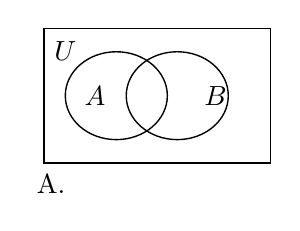
\begin{tikzpicture}[scale=0.9,line width=0.5pt]
\draw (0,0) rectangle (3.2,1.9);
\draw (1.02,0.95) ellipse (0.72 and 0.62);
\draw (1.88,0.95) ellipse (0.72 and 0.62);
\node at (0.72,0.95) {$A$};
\node at (2.42,0.95) {$B$};
\node at (0.3,1.58) {$U$};
\node[anchor=north] at (0.1,-0.03) {A.};
\end{tikzpicture}
&
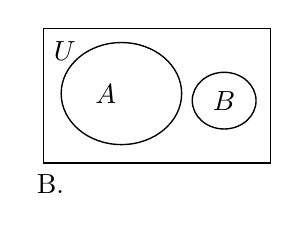
\begin{tikzpicture}[scale=0.9,line width=0.5pt]
\draw (0,0) rectangle (3.2,1.9);
\draw (1.1,0.98) ellipse (0.85 and 0.72);
\draw (2.55,0.88) ellipse (0.45 and 0.4);
\node at (0.88,0.98) {$A$};
\node at (2.55,0.88) {$B$};
\node at (0.3,1.58) {$U$};
\node[anchor=north] at (0.1,-0.03) {B.};
\end{tikzpicture}
\\[10pt]
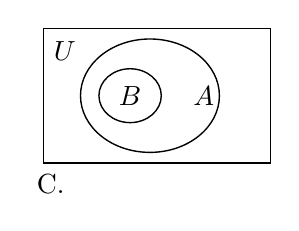
\begin{tikzpicture}[scale=0.9,line width=0.5pt]
\draw (0,0) rectangle (3.2,1.9);
\draw (1.5,0.95) ellipse (0.98 and 0.8);
\draw (1.22,0.95) ellipse (0.44 and 0.38);
\node at (1.22,0.95) {$B$};
\node at (2.26,0.95) {$A$};
\node at (0.3,1.58) {$U$};
\node[anchor=north] at (0.1,-0.03) {C.};
\end{tikzpicture}
&
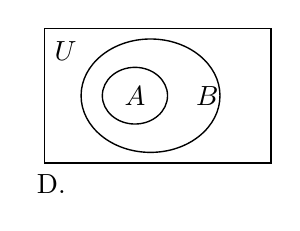
\begin{tikzpicture}[scale=0.9,line width=0.5pt]
\draw (0,0) rectangle (3.2,1.9);
\draw (1.5,0.95) ellipse (0.98 and 0.8);
\draw (1.28,0.95) ellipse (0.46 and 0.4);
\node at (1.28,0.95) {$A$};
\node at (2.3,0.95) {$B$};
\node at (0.3,1.58) {$U$};
\node[anchor=north] at (0.1,-0.03) {D.};
\end{tikzpicture}
\\
\end{tabular}
\end{center}

\ifanswer
\solbegin
\step{$\dfrac{2x-8}{x-5}\leqslant1\Rightarrow\dfrac{2x-8}{x-5}-1\leqslant0\Rightarrow\dfrac{x-3}{x-5}\leqslant0$，等价于 $\begin{cases}(x-3)(x-5)\leqslant0\\ x-5\neq0\end{cases}$，}
\step{解得 $3\leqslant x<5$，因为 $x\in\N$，所以 $A=\{3,4\}$，}
\step{解不等式 $x^2-7x+12\leqslant0$ 得 $B=\{x\mid3\leqslant x\leqslant4\}$，}
\step{集合 $A$ 中的元素 3，4 都属于集合 $B$，且 $B$ 中存在无数实数不属于 $A$，}
\step{所以 $A$ 是 $B$ 的真子集，$A$ 在 $B$ 内部．故选 $D$.}
\solend

\fi

\item 已知 $a$、$b$、$c\in\R$，则下列命题中真命题的个数是\mbox{（\quad）}

①若 $ac^2>bc^2$，则 $a>b$；②若 $\lvert a-2\rvert>\lvert b-2\rvert$，则 $(a-2)^2>(b-2)^2$；

③若 $a>b>c>0$，则 $\dfrac ab>\dfrac{a+c}{b+c}$；④若 $a>0$，$b>0$，$a+b>4$，$ab>4$，则 $a>2$，$b>2$.

\keepwithprev
A. $1$\qquad\qquad B. $2$\qquad\qquad C. $3$\qquad\qquad D. $4$

\ifanswer
\solbegin
\step{①若 $ac^2>bc^2$，则 $c^2>0$，则 $a>b$；所以①正确；}
\step{②若 $\lvert a-2\rvert>\lvert b-2\rvert$，则 $(a-2)^2>(b-2)^2$；满足不等式的基本性质，所以②正确；}
\step{③若 $a>b>c>0$，则 $\dfrac ab>\dfrac{a+c}{b+c}$；所以③正确；}
\step{④若 $a>0$，$b>0$，$a+b>4$，$ab>4$，则 $a>2$，$b>2$.}
\step{反例 $a=10$，$b=0.5$，满足条件，推不出结论，所以④不正确；}
\step{故选 $C$.}
\solend

\fi

\item 已知实数 $a<b$，关于 $x$ 的不等式 $x^2-(a+b)x+ab-1<0$ 的解集为 $(x_1,x_2)$，则实数
$a$、$b$、$x_1$、$x_2$ 从小到大的排列是\mbox{（\quad）}

\keepwithprev
A. $x_1<a<x_2<b$\qquad B. $x_1<a<b<x_2$\qquad C. $a<x_1<b<x_2$\qquad D. $a<x_1<x_2<b$

\ifanswer
\solbegin
\step{已知实数 $a<b$，关于 $x$ 的不等式 $x^2-(a+b)x+ab-1<0$ 的解集为 $(x_1,x_2)$，}
\step{因为 $x^2-(a+b)x+ab=(x-a)(x-b)$.}
\step{设函数 $g(x)=(x-a)(x-b)$，作函数 $g(x)$、$g(x)-1$ 的图象如下：}
\begin{center}
% 原图第 6 页解析插图直接裁取（原卷排于解析行右侧），已去粉色水印转灰度。
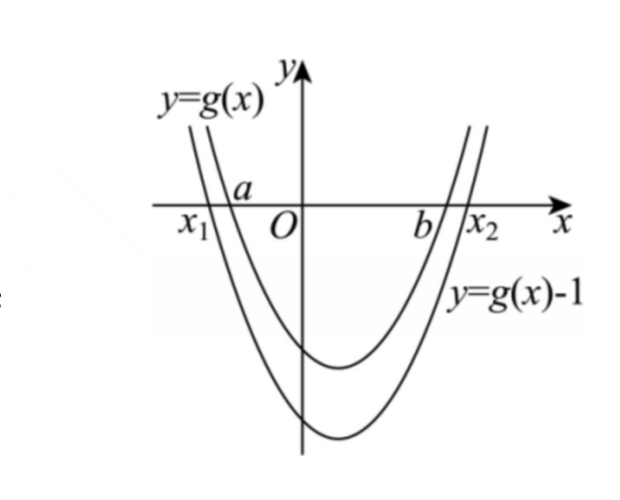
\includegraphics[width=0.20\textwidth]{figures/gao103_q16.png}
\end{center}
\step{由图像得 $x_1<a<b<x_2$．故选 $B$.}
\solend

\fi

\end{enumerate}

\bigsec{三、解答题}

\begin{enumerate}
\setcounter{enumi}{16}

\item 已知集合 $A=\{x\mid-3\leqslant x\leqslant1\}$，$B=\{x\mid a-2<x<a+2,a\in\R\}$.

（1）当 $a=1$ 时，求 $A\cap B$、$A\cup B$；

（2）若 $B\subseteq\overline A$，求 $a$ 的取值范围.

\ansspace*[8]

\ifanswer
\solbegin
\stepm{（1）}{当 $a=1$ 时，$B=\{x\mid-1<x<3\}$，又因为 $A=\{x\mid-3\leqslant x\leqslant1\}$，}
\step{所以 $A\cap B=\{x\mid-1<x\leqslant1\}$，$A\cup B=\{x\mid-3\leqslant x<3\}$；}
\stepm{（2）}{由 $A=\{x\mid-3\leqslant x\leqslant1\}$，得 $\overline A=\{x\mid x<-3\text{ 或 }x>1\}$，}
\step{若 $B\subseteq\overline A$，易得 $B=\{x\mid a-2<x<a+2,a\in\R\}\neq\varnothing$，}
\step{所以 $a+2\leqslant-3$ 或 $a-2\geqslant1$，解得 $a\leqslant-5$ 或 $a\geqslant3$，}
\step{综上所述，实数 $a$ 的取值范围是 $(-\infty,-5]\cup[3,+\infty)$.}
\solend

\fi

\item （1）解不等式 $\lvert 1-2x\rvert>x$；

（2）已知 $a$、$b$ 都是有理数，满足 $a+b\sqrt5=0$，请用反证法证明：$a=b=0$.

\ansspace*[10]

\ifanswer
\solbegin
\stepm{（1）}{①当 $x<0$ 时，左边非负，右边为负，不等式显然成立；}
\step{②当 $x\geqslant0$ 时，两边平方，$(1-2x)^2>x^2\Rightarrow3x^2-4x+1>0$}
\step{$\Rightarrow(3x-1)(x-1)>0$，解得 $x<\dfrac13$ 或 $x>1$，结合 $x\geqslant0$，}
\step{得 $0\leqslant x<\dfrac13$ 或 $x>1$；}
\step{综上，不等式解集为 $\left(-\infty,\dfrac13\right)\cup(1,+\infty)$.}
\stepm{（2）}{假设 $a,b$ 至少有一个不为零，}
\step{当 $a,b$ 中有一个为零一个不为零时，不妨设 $\begin{cases}a\neq0\\ b=0\end{cases}$，}
\step{则 $a+b\sqrt5=0\Rightarrow a=0$ 矛盾，舍；}
\step{当 $\begin{cases}a\neq0\\ b\neq0\end{cases}$ 时，$a+b\sqrt5=0\Rightarrow\sqrt5=-\dfrac ab\in\Q$，矛盾，舍，}
\step{综上假设不成立，所以 $a=b=0$.}
\solend

\fi

\item 某物流公司为了扩大业务量，计划建造一间高为 6 米，底面积为 24 平方米，且背面靠
墙的长方形形状的仓库。仓库的背面靠墙，无须建造费用，因此甲工程队给出的报价为：
仓库前面新建墙体每平方米 400 元，左右两面新建墙体每平方米 300 元，屋顶和地面以及
其他共计 28800 元.

（1）设仓库前面墙体的长为 $x$ 米 $(x>0)$，甲工程队的整体报价为 $y$ 元。若该物流公司计
划投入的改造资金不超过 60000 元，求前面墙体长 $x$ 的取值范围.

（2）在（1）的条件下，当仓库前面墙体的长度为多少时，甲工程队的整体
报价最低？

\begin{center}
% 原图第 7 页题干仓库示意图直接裁取（原卷排于题干右侧），已去粉色水印转灰度。
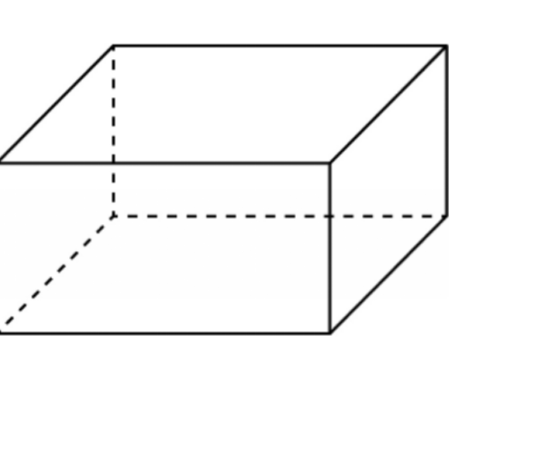
\includegraphics[width=0.17\textwidth]{figures/gao103_q19.png}
\end{center}

\ansspace*[12]

\ifanswer
\solbegin
\stepm{（1）}{甲队整体报价为 $y=400\times6x+2\times300\times6\times\dfrac{24}{x}+28800$}
\step{$=2400x+\dfrac{86400}{x}+28800$ 元，}
\step{要求 $y\leqslant60000$，即 $2400x+\dfrac{86400}{x}+28800\leqslant60000$，}
\step{化简得 $x+\dfrac{36}{x}\leqslant13$，}
\step{由于 $x>0$，则不等式化为 $x^2-13x+36\leqslant0$，}
\step{即 $(x-4)(x-9)\leqslant0$，解得 $4\leqslant x\leqslant9$，}
\step{所以前面墙体长 $x$ 的取值范围为 $[4,9]$；}
\stepm{（2）}{甲队整体报价为 $y=2400x+\dfrac{86400}{x}$}
\step{$\geqslant2\sqrt{2400x\times\dfrac{86400}{x}}+28800=57600$，}
\step{当且仅当 $2400x=\dfrac{86400}{x}$，即 $x^2=36$，}
\step{解得 $x=6$（满足 $4\leqslant x\leqslant9$）时取等号，}
\step{所以当仓库前面墙体的长度为 6 米时，甲工程队的整体报价最低，}
\step{为 57600 元.}
\solend

\fi

\item 已知函数 $f(x)=ax^2-10x+4b$.

（1）当 $a=1$，$b=4$ 时，解不等式 $f(x)\geqslant0$；

（2）若关于 $x$ 的不等式 $f(x)<0$ 的解集为 $(a,b)$，求实数 $a$、$b$ 的值；

（3）若 1 是 $f(x)$ 的零点，且 $a>0$，$b>0$，问当 $a$、$b$ 取何值时，$\dfrac1a+\dfrac1b$ 的值最小？最
小值是多少？

\ansspace*[12]

\ifanswer
\solbegin
\stepm{（1）}{将 $a=1$，$b=4$ 代入得 $f(x)=x^2-10x+16\geqslant0$，解得 $x\geqslant8$ 或 $x\leqslant2$，}
\step{所以不等式的解集为 $\{x\mid x\geqslant8\text{ 或 }x\leqslant2\}$；}
\stepm{（2）}{由题意得 $a$、$b$ 是 $ax^2-10x+4b=0$ 两根，且 $a<b$，$a>0$，}
\step{由韦达定理得 $\begin{cases}a+b=\dfrac{10}{a}\\ a\cdot b=\dfrac{4b}{a}\end{cases}$，解得 $\begin{cases}a=2\\ b=3\end{cases}$，即实数 $a$、$b$ 的值分别为 2，3；}
\stepm{（3）}{由 1 是 $f(x)$ 的零点，得 $f(1)=a-10+4b=0$，得 $a+4b=10$，}
\step{因为 $a>0$，$b>0$，}
\step{所以 $\dfrac1a+\dfrac1b=\dfrac1{10}\left(\dfrac1a+\dfrac1b\right)(a+4b)=\dfrac1{10}\left(1+4+\dfrac{4b}{a}+\dfrac ab\right)$}
\step{$\geqslant\dfrac1{10}\left(5+2\sqrt{\dfrac{4b}{a}\cdot\dfrac ab}\right)=\dfrac9{10}$，}
\step{当且仅当 $\dfrac{4b}{a}=\dfrac ab$，即 $a=\dfrac{10}3$,$b=\dfrac53$ 时取等号，}
\step{所以 $\dfrac1a+\dfrac1b$ 取最小值，且最小值为 $\dfrac9{10}$.}
\solend

\fi

\item 已知集合 $A$ 为非空集合，定义 $S=\{x\mid x=a+b,a,b\in A\}$，
$T=\{x\mid x=\lvert a-b\rvert,a,b\in A\}$.

（1）若集合 $A=\{1,3\}$，直接写出集合 $S$、$T$ (无需写计算过程)；

（2）若集合 $A=\{x_1,x_2,x_3,x_4\},x_1<x_2<x_3<x_4$，且 $T=A$，求证：$x_1+x_4=x_2+x_3$；

（3）若集合 $A=\{x\mid0\leqslant x\leqslant2026,x\in\N\}$,$S\cap T=\varnothing$．记 $\lvert A\rvert$ 为集合 $A$ 中元素的个数，求
$\lvert A\rvert$ 的最大值.

\ansspace*[16]

\ifanswer
\solbegin
\stepm{（1）}{$S=\{2,4,6\}$,$T=\{0,2\}$；}
\stepm{（2）}{集合 $T$ 中最小的元素为 0，因为 $T=A$，且 $x_1<x_2<x_3<x_4$，所以 $x_1=0$，}
\step{所以集合 $T$ 中元素为 $x_2-x_1=x_2$,$x_3-x_1=x_3$,$x_4-x_1=x_4$，}
\step{以及 $x_3-x_2$,$x_4-x_2$,$x_4-x_3$ 均属于 $A$，}
\step{因为 $x_1=0<x_3-x_2<x_4-x_2<x_4$，所以 $x_3$ 即 $x_4-x_2=x_3-x_1$，}
\step{即 $x_1+x_4=x_2+x_3$；}
\stepm{（3）}{设 $A=\{a_1,a_2,a_3,\cdots,a_k\}$ 满足题意，其中 $a_1<a_2<\cdots<a_k$，}
\step{则 $2a_1<a_1+a_2<\cdots<a_1+a_k<a_2+a_k<a_3+a_k<\cdots<a_{k-1}+a_k<2a_k$，}
\step{所以 $\lvert S\cup T\rvert\leqslant2k+1$，所以 $3k-1\leqslant2a_k+1\leqslant4053(k\in\N^*)$，}
\step{所以 $k\leqslant1351$，}
\step{实际上当 $A=\{676,677,\cdots,2026\}$ 时满足题意，}
\step{证明如下：设 $A=\{m,m+1,m+2,\cdots,2026\},m\in N$，}
\step{设 $S=\{2m,2m+1,2m+2,\cdots,4052\}$,$T=\{0,1,2,\cdots,2026-m\}$，}
\step{由题意得 $2026-m<2m$，即 $m>675\dfrac13$，}
\step{故 $m$ 的最小值是 676，于是当 $m=676$,$A$ 中的元素最多，}
\step{即 $A=\{676,677,\cdots,2026\}$ 时满足题意，}
\step{综上所述，集合 $A$ 中元素的个数的最大值是 1351.}
\solend

\fi

\end{enumerate}

\end{document}
"
%
% 原始材料：微信公众号“魔都数学加油站”文章，作者破晓，2026-11-01 21:56 发布；
% 连载“27学年高一103”，原文标题“27学年高一103——2026-2027年上海市市北中学高一上10月月考”；
% 原文链接：https://mp.weixin.qq.com/s/iBvF4eKw66F-kS6xLmDpBA。
% 正文为 10 张 PNG 页（第 1、3、5、6、7、10 页 2560×3620，其余 4762×6735），题目下印有【解析】，为讲评版。
% 题目、解析均据原图转录；卷面水印及公众号页脚未录入。
%
% 卷首标题：原卷印作“2026-2027 年市北中学高一上 10 月月考”（公众号标题中的“上海市”“高一上”
% 卷面标题行没有或已含，本稿照卷面），年份区间按全稿惯例排 en dash；原卷未印副标题，本稿按题目
% 内容标为“集合与常用逻辑用语、不等式”。
%
% 与原卷的排版差异：
%   ① 原文从第 3 题起，填空题编号为 3—12、选择题为 13—16、解答题为 17—21，本稿保留原题号；
%   ② 原卷每题下直接印【解析】，本稿按全稿惯例将解析置于答案版；选择题括号内未印答案，另由
%      解析末句“故选 X”给出；
%   ③ 原卷未印副标题，本稿按“知识模块”口径补出；
%   ④ 原卷填空横线按全稿惯例排为 \blankline[4.4em]；解答题按惯例加 \ansspace；选择题括号排
%      \mbox{（\quad）}；
%   ⑤ 原卷数集排斜体 $R$／$Q$（第 18 题解析 $Q$ 排粗体），按全稿惯例改 $\R$／$\Q$；
%   ⑥ 第 14 题四个文氏图选项按原图形状用 TikZ 重排；第 16、19 两题的插图裁自原图
%      （去粉色水印转灰度），第 19 题图属题干（三版都出），第 16 题图属解析（仅答案版显示）。
%
% 原卷存疑／笔误（均照录加注）：
%   第 9 题解析“故 $a+b=3b+b<0$”（$a=3b$ 代入应为 $4b$，原卷写作 $3b+b$，数值相同）；
%   第 21 题 (2) 解析“所以 $x_3$ 即 $x_4-x_2=x_3-x_1$”表述含糊（意为 $x_4-x_2$ 恰为 $T$ 中
%   介于 $x_2$ 与 $x_4$ 之间的元素 $x_3-x_1$）；
%   第 21 题 (3) 解析“所以 $|S\cup T|\leqslant2k+1$”（按上下文应为 $2a_k+1$，与后半句
%   $3k-1\leqslant2a_k+1$ 呼应），照录。
%
% 行数核对：逐题数 \step/\stepm 条数，合计 119 条（Q3：2；Q4：2；Q5：5；Q6：3；Q8：3；
% Q9：7；Q10：5；Q11：8；Q12：7；Q13：6；Q14：5；Q15：6；Q16：4；Q17：6；Q18：10；
% Q19：13；Q20：10；Q21：17），与原卷印刷行逐题相等。第 7 题只印【答案】，提 \ans{}，
% 不计入 \step 账。
%
\documentclass[a4paper,11pt]{article}
\usepackage{common}

\begin{document}

\examtitlest[3]{2026--2027 年市北中学高一上 10 月月考}{集合与常用逻辑用语、不等式}

\bigsec{一、填空题}

\begin{enumerate}
\setcounter{enumi}{2}

\item 已知实数 $x$ 满足 $\dfrac{7-x}{x+4}>0$，则 $x$ 的取值范围是\blankline[4.4em].

\ifanswer
\solbegin
\step{不等式 $\dfrac{7-x}{x+4}>0$ 可化为 $\dfrac{x-7}{x+4}<0$，等价于 $(x-7)(x+4)<0$，}
\step{解得 $-4<x<7$，所以 $x$ 的取值范围是 $\{x\mid-4<x<7\}$.}
\solend

\fi

\item 已知 $x_1$、$x_2$ 为方程 $2x^2+6x+3=0$ 的两个实数根，则 $\dfrac1{x_1}+\dfrac1{x_2}=$\blankline[4.4em].

\ifanswer
\solbegin
\step{由根与系数的关系得 $x_1+x_2=-\dfrac62=-3$，$x_1x_2=\dfrac32$，}
\step{则 $\dfrac1{x_1}+\dfrac1{x_2}=\dfrac{x_1+x_2}{x_1x_2}=-2$.}
\solend

\fi

\item 已知 $y=\lvert x-2\rvert+\lvert x-5\rvert$，$x\in\R$，则 $y$ 的最小值为\blankline[4.4em].

\ifanswer
\solbegin
\step{$y=\lvert x-2\rvert+\lvert x-5\rvert=\begin{cases}7-2x, & x<2\\ 3, & 2\leqslant x\leqslant5\\ 2x-7, & x>5\end{cases}$，}
\step{当 $x<2$ 时，$y>7-2\times2=3$；}
\step{当 $2\leqslant x\leqslant5$ 时，$y=3$；}
\step{当 $x>5$ 时，$y>2\times5-7=3$.}
\step{综上所述，$y$ 的最小值为 3.}
\solend

\fi

\item 对任意实数 $x$，等式 $ax^4+bx^3+cx^2+dx+e=x(x-2)(x^2+3)$ 恒成立，则
$b+c+d=$\blankline[4.4em].

\ifanswer
\solbegin
\step{因为 $ax^4+bx^3+cx^2+dx+e=x(x-2)(x^2+3)=(x^2-2x)(x^2+3)$}
\step{$=x^4-2x^3+3x^2-6x$，所以 $a=1$，$b=-2$，$c=3$，$d=-6$，$e=0$，}
\step{所以 $b+c+d=-2+3-6=-5$.}
\solend

\fi

\item 命题：“存在 $x\in(1,+\infty)$，使得 $ax^2+bx+c<0$”的否定形式是\blankline[4.4em].

\ifanswer
\ans{对于任意的 $x\in(1,+\infty)$，都有 $ax^2+bx+c\geqslant0$}
\fi

\item 已知集合 $A=\{x\mid mx^2-2x+1=0,x\in\R\}$ 有且仅有两个子集，则实数 $m=$\blankline[4.4em].

\ifanswer
\solbegin
\step{①当 $m=0$ 时，方程为 $-2x+1=0$，解得 $x=\dfrac12$，满足 $A=\left\{\dfrac12\right\}$ 仅有两个子集；}
\step{②当 $m\neq0$ 时，方程有两个相等实根，所以 $\Delta=4-4m=0$，解得 $m=1$；}
\step{所以实数 $m$ 的值为 0 或 1.}
\solend

\fi

\item 设 $a$、$b\in\R$，已知关于 $x$ 的不等式 $(a+b)x+(b-3a)<0$ 的解集为 $(2,+\infty)$，则不等式
$(a-2b)x+5b-a>0$ 的解集为\blankline[4.4em].

\ifanswer
\solbegin
\step{关于 $x$ 的不等式 $(a+b)x+(b-3a)<0$ 的解集为 $(2,+\infty)$，}
\step{得 $x=2$ 是 $(a+b)x+(b-3a)=0$ 的解，且 $a+b<0$，}
\step{所以 $2(a+b)+(b-3a)=0$，化简得 $a=3b$，故 $a+b=3b+b<0$，即 $b<0$，}
\step{将 $a=3b$ 代入 $(a-2b)x+5b-a>0$，}
\step{得不等式 $(a-2b)x+5b-a>0$ 即 $b(x+2)>0$，}
\step{两边都除以 $b$，得 $x+2<0$，解得 $x<-2$，}
\step{所以不等式 $(a-2b)x+5b-a>0$ 的解集为 $(-\infty,-2)$.}
\solend

\fi

\item 已知不等式 $\lvert x-a\rvert<1$ 成立的充分不必要条件是 $\dfrac12<x<\dfrac32$，则实数 $a$ 的取值范围
是\blankline[4.4em].

\ifanswer
\solbegin
\step{$\lvert x-a\rvert<1$，解得 $a-1<x<1+a$，}
\step{所以 $a-1<x<1+a$ 成立的充分不必要条件是 $\dfrac12<x<\dfrac32$，}
\step{故 $\left\{x\left|\dfrac12<x<\dfrac32\right.\right\}$ 是 $\{x\mid a-1<x<1+a\}$ 的真子集，}
\step{所以 $a-1\leqslant\dfrac12$ 且 $1+a\geqslant\dfrac32$（等号不同时成立），解得 $\dfrac12\leqslant a\leqslant\dfrac32$，}
\step{故实数 $a$ 的取值范围是 $\left[\dfrac12,\dfrac32\right]$.}
\solend

\fi

\item 定义 $A\nabla B=\left\{z\,\middle|\,z=xy+\dfrac xy,x\in A,y\in B\right\}$，设集合 $A=\{0,2\}$，$B=\{1,2\}$，$C=\{1\}$，
则集合 $(A\nabla B)\nabla C=$\blankline[4.4em].

\ifanswer
\solbegin
\step{当 $x=0$，$y=1$ 或 2 时，$z=xy+\dfrac xy=0$；}
\step{当 $x=2$，$y=1$ 时，$z=xy+\dfrac xy=4$；}
\step{当 $x=2$，$y=2$ 时，$z=xy+\dfrac xy=5$；}
\step{所以 $A\nabla B=\{0,4,5\}$；}
\step{当 $x=0$，$y=1$ 时，$z=xy+\dfrac xy=0$；}
\step{当 $x=4$，$y=1$ 时，$z=xy+\dfrac xy=8$；}
\step{当 $x=5$，$y=1$ 时，$z=xy+\dfrac xy=10$；}
\step{所以 $(A\nabla B)\nabla C=\{0,8,10\}$.}
\solend

\fi

\item 集合 $M=\{66,-11,23,10,911,-1,-18,100,0,\pi\}$ 有 10 个元素，设 $M$ 的所有非空子集为
$M_i\,(i=1,2,\cdots,1023)$，每一个 $M_i$ 中所有元素乘积为 $m_i\,(i=1,2,\cdots,1023)$，则
$m_1+m_2+m_3+\cdots+m_{1023}=$\blankline[4.4em].

\ifanswer
\solbegin
\step{因为 $M$ 的所有非空子集为 $M_i\,(i=1,2,\cdots,1023)$，这 1023 个子集分成以下几种情况：}
\step{①含 0 的子集有 512 个，这些子集均满足 $m_i=0$；}
\step{②不含 0，含 $-1$ 且还含有其它元素的子集有 255 个，}
\step{③不含 0，不含 $-1$ 但含有其它元素的子集有 255 个，}
\step{④只含 $-1$ 的子集一个 $\{-1\}$，满足 $m_i=-1$；}
\step{其中②③中的集合是一一对应的，且满足 $m_i$ 对应成相反数，}
\step{故 $m_1+m_2+m_3+\cdots+m_{1023}=512\times0+255\times0-1=-1$.}
\solend

\fi

\end{enumerate}

\bigsec{二、选择题}

\begin{enumerate}
\setcounter{enumi}{12}

\item 下列说法中，正确说法的个数是\mbox{（\quad）}

①联合国安理会常任理事国能组成一个集合；

②市北中学很喜欢足球的同学能组成一个集合；

③实数 $1,0,5,\dfrac12,\dfrac32,\dfrac64,\sqrt{\dfrac14}$ 组成的集合中有 6 个元素.

\keepwithprev
A. $0$\qquad\qquad B. $1$\qquad\qquad C. $2$\qquad\qquad D. $3$.

\ifanswer
\solbegin
\step{对于①，“联合国安理会常任理事国”满足集合的定义，故①正确；}
\step{对于②，“很喜欢”不满足集合的确定性，}
\step{市北中学很喜欢足球的同学不能组成一个集合，故②错误；}
\step{对于③，$\dfrac64=\dfrac32$，$\sqrt{\dfrac14}=\dfrac12$，由集合的元素互异性，集合中共有 5 个元素，}
\step{故③错误.}
\step{所以正确说法的个数是 1 个．故选 $B$.}
\solend

\fi

\item 已知全集 $U=\R$，集合 $A=\left\{x\,\middle|\,\dfrac{2x-8}{x-5}\leqslant1,x\in\N\right\}$，集合 $B=\{x\mid x^2-7x+12\leqslant0\}$，则
正确表示集合 $A$ 与集合 $B$ 关系的文氏图是\mbox{（\quad）}

\keepwithprev
\begin{center}
% 原卷四个文氏图选项按原图形状用 TikZ 重排。
\begin{tabular}{c@{\qquad\qquad}c}
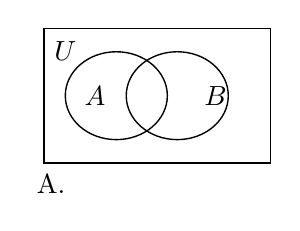
\begin{tikzpicture}[scale=0.9,line width=0.5pt]
\draw (0,0) rectangle (3.2,1.9);
\draw (1.02,0.95) ellipse (0.72 and 0.62);
\draw (1.88,0.95) ellipse (0.72 and 0.62);
\node at (0.72,0.95) {$A$};
\node at (2.42,0.95) {$B$};
\node at (0.3,1.58) {$U$};
\node[anchor=north] at (0.1,-0.03) {A.};
\end{tikzpicture}
&
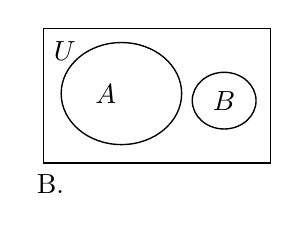
\begin{tikzpicture}[scale=0.9,line width=0.5pt]
\draw (0,0) rectangle (3.2,1.9);
\draw (1.1,0.98) ellipse (0.85 and 0.72);
\draw (2.55,0.88) ellipse (0.45 and 0.4);
\node at (0.88,0.98) {$A$};
\node at (2.55,0.88) {$B$};
\node at (0.3,1.58) {$U$};
\node[anchor=north] at (0.1,-0.03) {B.};
\end{tikzpicture}
\\[10pt]
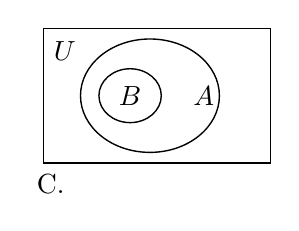
\begin{tikzpicture}[scale=0.9,line width=0.5pt]
\draw (0,0) rectangle (3.2,1.9);
\draw (1.5,0.95) ellipse (0.98 and 0.8);
\draw (1.22,0.95) ellipse (0.44 and 0.38);
\node at (1.22,0.95) {$B$};
\node at (2.26,0.95) {$A$};
\node at (0.3,1.58) {$U$};
\node[anchor=north] at (0.1,-0.03) {C.};
\end{tikzpicture}
&
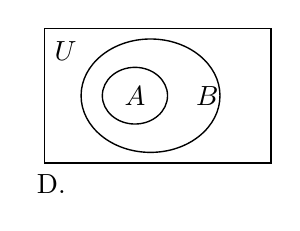
\begin{tikzpicture}[scale=0.9,line width=0.5pt]
\draw (0,0) rectangle (3.2,1.9);
\draw (1.5,0.95) ellipse (0.98 and 0.8);
\draw (1.28,0.95) ellipse (0.46 and 0.4);
\node at (1.28,0.95) {$A$};
\node at (2.3,0.95) {$B$};
\node at (0.3,1.58) {$U$};
\node[anchor=north] at (0.1,-0.03) {D.};
\end{tikzpicture}
\\
\end{tabular}
\end{center}

\ifanswer
\solbegin
\step{$\dfrac{2x-8}{x-5}\leqslant1\Rightarrow\dfrac{2x-8}{x-5}-1\leqslant0\Rightarrow\dfrac{x-3}{x-5}\leqslant0$，等价于 $\begin{cases}(x-3)(x-5)\leqslant0\\ x-5\neq0\end{cases}$，}
\step{解得 $3\leqslant x<5$，因为 $x\in\N$，所以 $A=\{3,4\}$，}
\step{解不等式 $x^2-7x+12\leqslant0$ 得 $B=\{x\mid3\leqslant x\leqslant4\}$，}
\step{集合 $A$ 中的元素 3，4 都属于集合 $B$，且 $B$ 中存在无数实数不属于 $A$，}
\step{所以 $A$ 是 $B$ 的真子集，$A$ 在 $B$ 内部．故选 $D$.}
\solend

\fi

\item 已知 $a$、$b$、$c\in\R$，则下列命题中真命题的个数是\mbox{（\quad）}

①若 $ac^2>bc^2$，则 $a>b$；②若 $\lvert a-2\rvert>\lvert b-2\rvert$，则 $(a-2)^2>(b-2)^2$；

③若 $a>b>c>0$，则 $\dfrac ab>\dfrac{a+c}{b+c}$；④若 $a>0$，$b>0$，$a+b>4$，$ab>4$，则 $a>2$，$b>2$.

\keepwithprev
A. $1$\qquad\qquad B. $2$\qquad\qquad C. $3$\qquad\qquad D. $4$

\ifanswer
\solbegin
\step{①若 $ac^2>bc^2$，则 $c^2>0$，则 $a>b$；所以①正确；}
\step{②若 $\lvert a-2\rvert>\lvert b-2\rvert$，则 $(a-2)^2>(b-2)^2$；满足不等式的基本性质，所以②正确；}
\step{③若 $a>b>c>0$，则 $\dfrac ab>\dfrac{a+c}{b+c}$；所以③正确；}
\step{④若 $a>0$，$b>0$，$a+b>4$，$ab>4$，则 $a>2$，$b>2$.}
\step{反例 $a=10$，$b=0.5$，满足条件，推不出结论，所以④不正确；}
\step{故选 $C$.}
\solend

\fi

\item 已知实数 $a<b$，关于 $x$ 的不等式 $x^2-(a+b)x+ab-1<0$ 的解集为 $(x_1,x_2)$，则实数
$a$、$b$、$x_1$、$x_2$ 从小到大的排列是\mbox{（\quad）}

\keepwithprev
A. $x_1<a<x_2<b$\qquad B. $x_1<a<b<x_2$\qquad C. $a<x_1<b<x_2$\qquad D. $a<x_1<x_2<b$

\ifanswer
\solbegin
\step{已知实数 $a<b$，关于 $x$ 的不等式 $x^2-(a+b)x+ab-1<0$ 的解集为 $(x_1,x_2)$，}
\step{因为 $x^2-(a+b)x+ab=(x-a)(x-b)$.}
\step{设函数 $g(x)=(x-a)(x-b)$，作函数 $g(x)$、$g(x)-1$ 的图象如下：}
\begin{center}
% 原图第 6 页解析插图直接裁取（原卷排于解析行右侧），已去粉色水印转灰度。
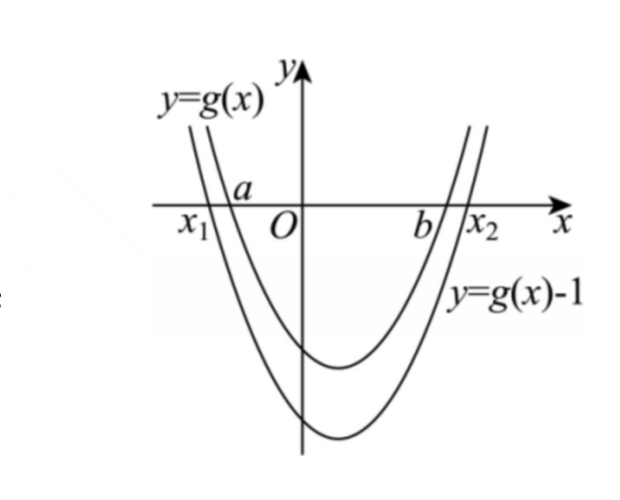
\includegraphics[width=0.20\textwidth]{figures/gao103_q16.png}
\end{center}
\step{由图像得 $x_1<a<b<x_2$．故选 $B$.}
\solend

\fi

\end{enumerate}

\bigsec{三、解答题}

\begin{enumerate}
\setcounter{enumi}{16}

\item 已知集合 $A=\{x\mid-3\leqslant x\leqslant1\}$，$B=\{x\mid a-2<x<a+2,a\in\R\}$.

（1）当 $a=1$ 时，求 $A\cap B$、$A\cup B$；

（2）若 $B\subseteq\overline A$，求 $a$ 的取值范围.

\ansspace*[8]

\ifanswer
\solbegin
\stepm{（1）}{当 $a=1$ 时，$B=\{x\mid-1<x<3\}$，又因为 $A=\{x\mid-3\leqslant x\leqslant1\}$，}
\step{所以 $A\cap B=\{x\mid-1<x\leqslant1\}$，$A\cup B=\{x\mid-3\leqslant x<3\}$；}
\stepm{（2）}{由 $A=\{x\mid-3\leqslant x\leqslant1\}$，得 $\overline A=\{x\mid x<-3\text{ 或 }x>1\}$，}
\step{若 $B\subseteq\overline A$，易得 $B=\{x\mid a-2<x<a+2,a\in\R\}\neq\varnothing$，}
\step{所以 $a+2\leqslant-3$ 或 $a-2\geqslant1$，解得 $a\leqslant-5$ 或 $a\geqslant3$，}
\step{综上所述，实数 $a$ 的取值范围是 $(-\infty,-5]\cup[3,+\infty)$.}
\solend

\fi

\item （1）解不等式 $\lvert 1-2x\rvert>x$；

（2）已知 $a$、$b$ 都是有理数，满足 $a+b\sqrt5=0$，请用反证法证明：$a=b=0$.

\ansspace*[10]

\ifanswer
\solbegin
\stepm{（1）}{①当 $x<0$ 时，左边非负，右边为负，不等式显然成立；}
\step{②当 $x\geqslant0$ 时，两边平方，$(1-2x)^2>x^2\Rightarrow3x^2-4x+1>0$}
\step{$\Rightarrow(3x-1)(x-1)>0$，解得 $x<\dfrac13$ 或 $x>1$，结合 $x\geqslant0$，}
\step{得 $0\leqslant x<\dfrac13$ 或 $x>1$；}
\step{综上，不等式解集为 $\left(-\infty,\dfrac13\right)\cup(1,+\infty)$.}
\stepm{（2）}{假设 $a,b$ 至少有一个不为零，}
\step{当 $a,b$ 中有一个为零一个不为零时，不妨设 $\begin{cases}a\neq0\\ b=0\end{cases}$，}
\step{则 $a+b\sqrt5=0\Rightarrow a=0$ 矛盾，舍；}
\step{当 $\begin{cases}a\neq0\\ b\neq0\end{cases}$ 时，$a+b\sqrt5=0\Rightarrow\sqrt5=-\dfrac ab\in\Q$，矛盾，舍，}
\step{综上假设不成立，所以 $a=b=0$.}
\solend

\fi

\item 某物流公司为了扩大业务量，计划建造一间高为 6 米，底面积为 24 平方米，且背面靠
墙的长方形形状的仓库。仓库的背面靠墙，无须建造费用，因此甲工程队给出的报价为：
仓库前面新建墙体每平方米 400 元，左右两面新建墙体每平方米 300 元，屋顶和地面以及
其他共计 28800 元.

（1）设仓库前面墙体的长为 $x$ 米 $(x>0)$，甲工程队的整体报价为 $y$ 元。若该物流公司计
划投入的改造资金不超过 60000 元，求前面墙体长 $x$ 的取值范围.

（2）在（1）的条件下，当仓库前面墙体的长度为多少时，甲工程队的整体
报价最低？

\begin{center}
% 原图第 7 页题干仓库示意图直接裁取（原卷排于题干右侧），已去粉色水印转灰度。
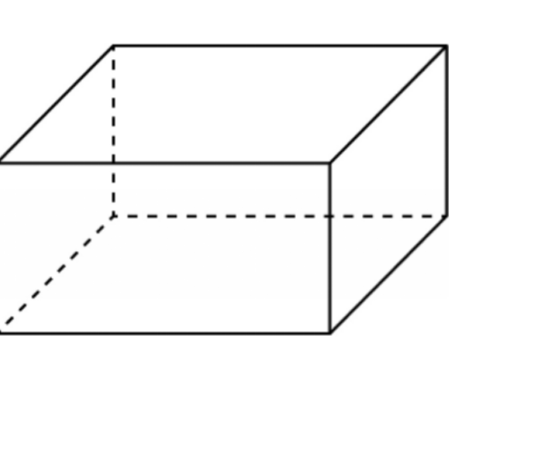
\includegraphics[width=0.17\textwidth]{figures/gao103_q19.png}
\end{center}

\ansspace*[12]

\ifanswer
\solbegin
\stepm{（1）}{甲队整体报价为 $y=400\times6x+2\times300\times6\times\dfrac{24}{x}+28800$}
\step{$=2400x+\dfrac{86400}{x}+28800$ 元，}
\step{要求 $y\leqslant60000$，即 $2400x+\dfrac{86400}{x}+28800\leqslant60000$，}
\step{化简得 $x+\dfrac{36}{x}\leqslant13$，}
\step{由于 $x>0$，则不等式化为 $x^2-13x+36\leqslant0$，}
\step{即 $(x-4)(x-9)\leqslant0$，解得 $4\leqslant x\leqslant9$，}
\step{所以前面墙体长 $x$ 的取值范围为 $[4,9]$；}
\stepm{（2）}{甲队整体报价为 $y=2400x+\dfrac{86400}{x}$}
\step{$\geqslant2\sqrt{2400x\times\dfrac{86400}{x}}+28800=57600$，}
\step{当且仅当 $2400x=\dfrac{86400}{x}$，即 $x^2=36$，}
\step{解得 $x=6$（满足 $4\leqslant x\leqslant9$）时取等号，}
\step{所以当仓库前面墙体的长度为 6 米时，甲工程队的整体报价最低，}
\step{为 57600 元.}
\solend

\fi

\item 已知函数 $f(x)=ax^2-10x+4b$.

（1）当 $a=1$，$b=4$ 时，解不等式 $f(x)\geqslant0$；

（2）若关于 $x$ 的不等式 $f(x)<0$ 的解集为 $(a,b)$，求实数 $a$、$b$ 的值；

（3）若 1 是 $f(x)$ 的零点，且 $a>0$，$b>0$，问当 $a$、$b$ 取何值时，$\dfrac1a+\dfrac1b$ 的值最小？最
小值是多少？

\ansspace*[12]

\ifanswer
\solbegin
\stepm{（1）}{将 $a=1$，$b=4$ 代入得 $f(x)=x^2-10x+16\geqslant0$，解得 $x\geqslant8$ 或 $x\leqslant2$，}
\step{所以不等式的解集为 $\{x\mid x\geqslant8\text{ 或 }x\leqslant2\}$；}
\stepm{（2）}{由题意得 $a$、$b$ 是 $ax^2-10x+4b=0$ 两根，且 $a<b$，$a>0$，}
\step{由韦达定理得 $\begin{cases}a+b=\dfrac{10}{a}\\ a\cdot b=\dfrac{4b}{a}\end{cases}$，解得 $\begin{cases}a=2\\ b=3\end{cases}$，即实数 $a$、$b$ 的值分别为 2，3；}
\stepm{（3）}{由 1 是 $f(x)$ 的零点，得 $f(1)=a-10+4b=0$，得 $a+4b=10$，}
\step{因为 $a>0$，$b>0$，}
\step{所以 $\dfrac1a+\dfrac1b=\dfrac1{10}\left(\dfrac1a+\dfrac1b\right)(a+4b)=\dfrac1{10}\left(1+4+\dfrac{4b}{a}+\dfrac ab\right)$}
\step{$\geqslant\dfrac1{10}\left(5+2\sqrt{\dfrac{4b}{a}\cdot\dfrac ab}\right)=\dfrac9{10}$，}
\step{当且仅当 $\dfrac{4b}{a}=\dfrac ab$，即 $a=\dfrac{10}3$,$b=\dfrac53$ 时取等号，}
\step{所以 $\dfrac1a+\dfrac1b$ 取最小值，且最小值为 $\dfrac9{10}$.}
\solend

\fi

\item 已知集合 $A$ 为非空集合，定义 $S=\{x\mid x=a+b,a,b\in A\}$，
$T=\{x\mid x=\lvert a-b\rvert,a,b\in A\}$.

（1）若集合 $A=\{1,3\}$，直接写出集合 $S$、$T$ (无需写计算过程)；

（2）若集合 $A=\{x_1,x_2,x_3,x_4\},x_1<x_2<x_3<x_4$，且 $T=A$，求证：$x_1+x_4=x_2+x_3$；

（3）若集合 $A=\{x\mid0\leqslant x\leqslant2026,x\in\N\}$,$S\cap T=\varnothing$．记 $\lvert A\rvert$ 为集合 $A$ 中元素的个数，求
$\lvert A\rvert$ 的最大值.

\ansspace*[16]

\ifanswer
\solbegin
\stepm{（1）}{$S=\{2,4,6\}$,$T=\{0,2\}$；}
\stepm{（2）}{集合 $T$ 中最小的元素为 0，因为 $T=A$，且 $x_1<x_2<x_3<x_4$，所以 $x_1=0$，}
\step{所以集合 $T$ 中元素为 $x_2-x_1=x_2$,$x_3-x_1=x_3$,$x_4-x_1=x_4$，}
\step{以及 $x_3-x_2$,$x_4-x_2$,$x_4-x_3$ 均属于 $A$，}
\step{因为 $x_1=0<x_3-x_2<x_4-x_2<x_4$，所以 $x_3$ 即 $x_4-x_2=x_3-x_1$，}
\step{即 $x_1+x_4=x_2+x_3$；}
\stepm{（3）}{设 $A=\{a_1,a_2,a_3,\cdots,a_k\}$ 满足题意，其中 $a_1<a_2<\cdots<a_k$，}
\step{则 $2a_1<a_1+a_2<\cdots<a_1+a_k<a_2+a_k<a_3+a_k<\cdots<a_{k-1}+a_k<2a_k$，}
\step{所以 $\lvert S\cup T\rvert\leqslant2k+1$，所以 $3k-1\leqslant2a_k+1\leqslant4053(k\in\N^*)$，}
\step{所以 $k\leqslant1351$，}
\step{实际上当 $A=\{676,677,\cdots,2026\}$ 时满足题意，}
\step{证明如下：设 $A=\{m,m+1,m+2,\cdots,2026\},m\in N$，}
\step{设 $S=\{2m,2m+1,2m+2,\cdots,4052\}$,$T=\{0,1,2,\cdots,2026-m\}$，}
\step{由题意得 $2026-m<2m$，即 $m>675\dfrac13$，}
\step{故 $m$ 的最小值是 676，于是当 $m=676$,$A$ 中的元素最多，}
\step{即 $A=\{676,677,\cdots,2026\}$ 时满足题意，}
\step{综上所述，集合 $A$ 中元素的个数的最大值是 1351.}
\solend

\fi

\end{enumerate}

\end{document}
"
%
% 原始材料：微信公众号“魔都数学加油站”文章，作者破晓，2026-11-01 21:56 发布；
% 连载“27学年高一103”，原文标题“27学年高一103——2026-2027年上海市市北中学高一上10月月考”；
% 原文链接：https://mp.weixin.qq.com/s/iBvF4eKw66F-kS6xLmDpBA。
% 正文为 10 张 PNG 页（第 1、3、5、6、7、10 页 2560×3620，其余 4762×6735），题目下印有【解析】，为讲评版。
% 题目、解析均据原图转录；卷面水印及公众号页脚未录入。
%
% 卷首标题：原卷印作“2026-2027 年市北中学高一上 10 月月考”（公众号标题中的“上海市”“高一上”
% 卷面标题行没有或已含，本稿照卷面），年份区间按全稿惯例排 en dash；原卷未印副标题，本稿按题目
% 内容标为“集合与常用逻辑用语、不等式”。
%
% 与原卷的排版差异：
%   ① 原文从第 3 题起，填空题编号为 3—12、选择题为 13—16、解答题为 17—21，本稿保留原题号；
%   ② 原卷每题下直接印【解析】，本稿按全稿惯例将解析置于答案版；选择题括号内未印答案，另由
%      解析末句“故选 X”给出；
%   ③ 原卷未印副标题，本稿按“知识模块”口径补出；
%   ④ 原卷填空横线按全稿惯例排为 \blankline[4.4em]；解答题按惯例加 \ansspace；选择题括号排
%      \mbox{（\quad）}；
%   ⑤ 原卷数集排斜体 $R$／$Q$（第 18 题解析 $Q$ 排粗体），按全稿惯例改 $\R$／$\Q$；
%   ⑥ 第 14 题四个文氏图选项按原图形状用 TikZ 重排；第 16、19 两题的插图裁自原图
%      （去粉色水印转灰度），第 19 题图属题干（三版都出），第 16 题图属解析（仅答案版显示）。
%
% 原卷存疑／笔误（均照录加注）：
%   第 9 题解析“故 $a+b=3b+b<0$”（$a=3b$ 代入应为 $4b$，原卷写作 $3b+b$，数值相同）；
%   第 21 题 (2) 解析“所以 $x_3$ 即 $x_4-x_2=x_3-x_1$”表述含糊（意为 $x_4-x_2$ 恰为 $T$ 中
%   介于 $x_2$ 与 $x_4$ 之间的元素 $x_3-x_1$）；
%   第 21 题 (3) 解析“所以 $|S\cup T|\leqslant2k+1$”（按上下文应为 $2a_k+1$，与后半句
%   $3k-1\leqslant2a_k+1$ 呼应），照录。
%
% 行数核对：逐题数 \step/\stepm 条数，合计 119 条（Q3：2；Q4：2；Q5：5；Q6：3；Q8：3；
% Q9：7；Q10：5；Q11：8；Q12：7；Q13：6；Q14：5；Q15：6；Q16：4；Q17：6；Q18：10；
% Q19：13；Q20：10；Q21：17），与原卷印刷行逐题相等。第 7 题只印【答案】，提 \ans{}，
% 不计入 \step 账。
%
\documentclass[a4paper,11pt]{article}
\usepackage{common}

\begin{document}

\examtitlest[3]{2026--2027 年市北中学高一上 10 月月考}{集合与常用逻辑用语、不等式}

\bigsec{一、填空题}

\begin{enumerate}
\setcounter{enumi}{2}

\item 已知实数 $x$ 满足 $\dfrac{7-x}{x+4}>0$，则 $x$ 的取值范围是\blankline[4.4em].

\ifanswer
\solbegin
\step{不等式 $\dfrac{7-x}{x+4}>0$ 可化为 $\dfrac{x-7}{x+4}<0$，等价于 $(x-7)(x+4)<0$，}
\step{解得 $-4<x<7$，所以 $x$ 的取值范围是 $\{x\mid-4<x<7\}$.}
\solend

\fi

\item 已知 $x_1$、$x_2$ 为方程 $2x^2+6x+3=0$ 的两个实数根，则 $\dfrac1{x_1}+\dfrac1{x_2}=$\blankline[4.4em].

\ifanswer
\solbegin
\step{由根与系数的关系得 $x_1+x_2=-\dfrac62=-3$，$x_1x_2=\dfrac32$，}
\step{则 $\dfrac1{x_1}+\dfrac1{x_2}=\dfrac{x_1+x_2}{x_1x_2}=-2$.}
\solend

\fi

\item 已知 $y=\lvert x-2\rvert+\lvert x-5\rvert$，$x\in\R$，则 $y$ 的最小值为\blankline[4.4em].

\ifanswer
\solbegin
\step{$y=\lvert x-2\rvert+\lvert x-5\rvert=\begin{cases}7-2x, & x<2\\ 3, & 2\leqslant x\leqslant5\\ 2x-7, & x>5\end{cases}$，}
\step{当 $x<2$ 时，$y>7-2\times2=3$；}
\step{当 $2\leqslant x\leqslant5$ 时，$y=3$；}
\step{当 $x>5$ 时，$y>2\times5-7=3$.}
\step{综上所述，$y$ 的最小值为 3.}
\solend

\fi

\item 对任意实数 $x$，等式 $ax^4+bx^3+cx^2+dx+e=x(x-2)(x^2+3)$ 恒成立，则
$b+c+d=$\blankline[4.4em].

\ifanswer
\solbegin
\step{因为 $ax^4+bx^3+cx^2+dx+e=x(x-2)(x^2+3)=(x^2-2x)(x^2+3)$}
\step{$=x^4-2x^3+3x^2-6x$，所以 $a=1$，$b=-2$，$c=3$，$d=-6$，$e=0$，}
\step{所以 $b+c+d=-2+3-6=-5$.}
\solend

\fi

\item 命题：“存在 $x\in(1,+\infty)$，使得 $ax^2+bx+c<0$”的否定形式是\blankline[4.4em].

\ifanswer
\ans{对于任意的 $x\in(1,+\infty)$，都有 $ax^2+bx+c\geqslant0$}
\fi

\item 已知集合 $A=\{x\mid mx^2-2x+1=0,x\in\R\}$ 有且仅有两个子集，则实数 $m=$\blankline[4.4em].

\ifanswer
\solbegin
\step{①当 $m=0$ 时，方程为 $-2x+1=0$，解得 $x=\dfrac12$，满足 $A=\left\{\dfrac12\right\}$ 仅有两个子集；}
\step{②当 $m\neq0$ 时，方程有两个相等实根，所以 $\Delta=4-4m=0$，解得 $m=1$；}
\step{所以实数 $m$ 的值为 0 或 1.}
\solend

\fi

\item 设 $a$、$b\in\R$，已知关于 $x$ 的不等式 $(a+b)x+(b-3a)<0$ 的解集为 $(2,+\infty)$，则不等式
$(a-2b)x+5b-a>0$ 的解集为\blankline[4.4em].

\ifanswer
\solbegin
\step{关于 $x$ 的不等式 $(a+b)x+(b-3a)<0$ 的解集为 $(2,+\infty)$，}
\step{得 $x=2$ 是 $(a+b)x+(b-3a)=0$ 的解，且 $a+b<0$，}
\step{所以 $2(a+b)+(b-3a)=0$，化简得 $a=3b$，故 $a+b=3b+b<0$，即 $b<0$，}
\step{将 $a=3b$ 代入 $(a-2b)x+5b-a>0$，}
\step{得不等式 $(a-2b)x+5b-a>0$ 即 $b(x+2)>0$，}
\step{两边都除以 $b$，得 $x+2<0$，解得 $x<-2$，}
\step{所以不等式 $(a-2b)x+5b-a>0$ 的解集为 $(-\infty,-2)$.}
\solend

\fi

\item 已知不等式 $\lvert x-a\rvert<1$ 成立的充分不必要条件是 $\dfrac12<x<\dfrac32$，则实数 $a$ 的取值范围
是\blankline[4.4em].

\ifanswer
\solbegin
\step{$\lvert x-a\rvert<1$，解得 $a-1<x<1+a$，}
\step{所以 $a-1<x<1+a$ 成立的充分不必要条件是 $\dfrac12<x<\dfrac32$，}
\step{故 $\left\{x\left|\dfrac12<x<\dfrac32\right.\right\}$ 是 $\{x\mid a-1<x<1+a\}$ 的真子集，}
\step{所以 $a-1\leqslant\dfrac12$ 且 $1+a\geqslant\dfrac32$（等号不同时成立），解得 $\dfrac12\leqslant a\leqslant\dfrac32$，}
\step{故实数 $a$ 的取值范围是 $\left[\dfrac12,\dfrac32\right]$.}
\solend

\fi

\item 定义 $A\nabla B=\left\{z\,\middle|\,z=xy+\dfrac xy,x\in A,y\in B\right\}$，设集合 $A=\{0,2\}$，$B=\{1,2\}$，$C=\{1\}$，
则集合 $(A\nabla B)\nabla C=$\blankline[4.4em].

\ifanswer
\solbegin
\step{当 $x=0$，$y=1$ 或 2 时，$z=xy+\dfrac xy=0$；}
\step{当 $x=2$，$y=1$ 时，$z=xy+\dfrac xy=4$；}
\step{当 $x=2$，$y=2$ 时，$z=xy+\dfrac xy=5$；}
\step{所以 $A\nabla B=\{0,4,5\}$；}
\step{当 $x=0$，$y=1$ 时，$z=xy+\dfrac xy=0$；}
\step{当 $x=4$，$y=1$ 时，$z=xy+\dfrac xy=8$；}
\step{当 $x=5$，$y=1$ 时，$z=xy+\dfrac xy=10$；}
\step{所以 $(A\nabla B)\nabla C=\{0,8,10\}$.}
\solend

\fi

\item 集合 $M=\{66,-11,23,10,911,-1,-18,100,0,\pi\}$ 有 10 个元素，设 $M$ 的所有非空子集为
$M_i\,(i=1,2,\cdots,1023)$，每一个 $M_i$ 中所有元素乘积为 $m_i\,(i=1,2,\cdots,1023)$，则
$m_1+m_2+m_3+\cdots+m_{1023}=$\blankline[4.4em].

\ifanswer
\solbegin
\step{因为 $M$ 的所有非空子集为 $M_i\,(i=1,2,\cdots,1023)$，这 1023 个子集分成以下几种情况：}
\step{①含 0 的子集有 512 个，这些子集均满足 $m_i=0$；}
\step{②不含 0，含 $-1$ 且还含有其它元素的子集有 255 个，}
\step{③不含 0，不含 $-1$ 但含有其它元素的子集有 255 个，}
\step{④只含 $-1$ 的子集一个 $\{-1\}$，满足 $m_i=-1$；}
\step{其中②③中的集合是一一对应的，且满足 $m_i$ 对应成相反数，}
\step{故 $m_1+m_2+m_3+\cdots+m_{1023}=512\times0+255\times0-1=-1$.}
\solend

\fi

\end{enumerate}

\bigsec{二、选择题}

\begin{enumerate}
\setcounter{enumi}{12}

\item 下列说法中，正确说法的个数是\mbox{（\quad）}

①联合国安理会常任理事国能组成一个集合；

②市北中学很喜欢足球的同学能组成一个集合；

③实数 $1,0,5,\dfrac12,\dfrac32,\dfrac64,\sqrt{\dfrac14}$ 组成的集合中有 6 个元素.

\keepwithprev
A. $0$\qquad\qquad B. $1$\qquad\qquad C. $2$\qquad\qquad D. $3$.

\ifanswer
\solbegin
\step{对于①，“联合国安理会常任理事国”满足集合的定义，故①正确；}
\step{对于②，“很喜欢”不满足集合的确定性，}
\step{市北中学很喜欢足球的同学不能组成一个集合，故②错误；}
\step{对于③，$\dfrac64=\dfrac32$，$\sqrt{\dfrac14}=\dfrac12$，由集合的元素互异性，集合中共有 5 个元素，}
\step{故③错误.}
\step{所以正确说法的个数是 1 个．故选 $B$.}
\solend

\fi

\item 已知全集 $U=\R$，集合 $A=\left\{x\,\middle|\,\dfrac{2x-8}{x-5}\leqslant1,x\in\N\right\}$，集合 $B=\{x\mid x^2-7x+12\leqslant0\}$，则
正确表示集合 $A$ 与集合 $B$ 关系的文氏图是\mbox{（\quad）}

\keepwithprev
\begin{center}
% 原卷四个文氏图选项按原图形状用 TikZ 重排。
\begin{tabular}{c@{\qquad\qquad}c}
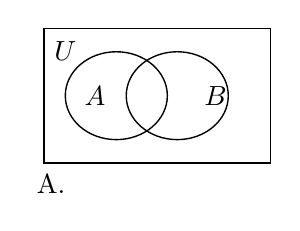
\begin{tikzpicture}[scale=0.9,line width=0.5pt]
\draw (0,0) rectangle (3.2,1.9);
\draw (1.02,0.95) ellipse (0.72 and 0.62);
\draw (1.88,0.95) ellipse (0.72 and 0.62);
\node at (0.72,0.95) {$A$};
\node at (2.42,0.95) {$B$};
\node at (0.3,1.58) {$U$};
\node[anchor=north] at (0.1,-0.03) {A.};
\end{tikzpicture}
&
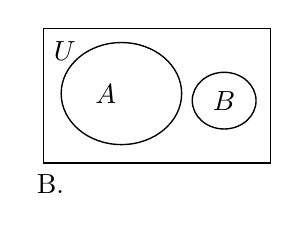
\begin{tikzpicture}[scale=0.9,line width=0.5pt]
\draw (0,0) rectangle (3.2,1.9);
\draw (1.1,0.98) ellipse (0.85 and 0.72);
\draw (2.55,0.88) ellipse (0.45 and 0.4);
\node at (0.88,0.98) {$A$};
\node at (2.55,0.88) {$B$};
\node at (0.3,1.58) {$U$};
\node[anchor=north] at (0.1,-0.03) {B.};
\end{tikzpicture}
\\[10pt]
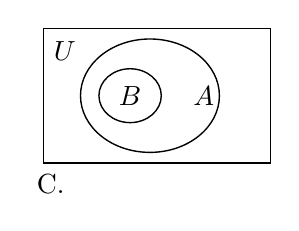
\begin{tikzpicture}[scale=0.9,line width=0.5pt]
\draw (0,0) rectangle (3.2,1.9);
\draw (1.5,0.95) ellipse (0.98 and 0.8);
\draw (1.22,0.95) ellipse (0.44 and 0.38);
\node at (1.22,0.95) {$B$};
\node at (2.26,0.95) {$A$};
\node at (0.3,1.58) {$U$};
\node[anchor=north] at (0.1,-0.03) {C.};
\end{tikzpicture}
&
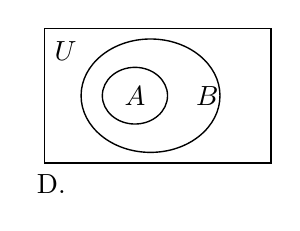
\begin{tikzpicture}[scale=0.9,line width=0.5pt]
\draw (0,0) rectangle (3.2,1.9);
\draw (1.5,0.95) ellipse (0.98 and 0.8);
\draw (1.28,0.95) ellipse (0.46 and 0.4);
\node at (1.28,0.95) {$A$};
\node at (2.3,0.95) {$B$};
\node at (0.3,1.58) {$U$};
\node[anchor=north] at (0.1,-0.03) {D.};
\end{tikzpicture}
\\
\end{tabular}
\end{center}

\ifanswer
\solbegin
\step{$\dfrac{2x-8}{x-5}\leqslant1\Rightarrow\dfrac{2x-8}{x-5}-1\leqslant0\Rightarrow\dfrac{x-3}{x-5}\leqslant0$，等价于 $\begin{cases}(x-3)(x-5)\leqslant0\\ x-5\neq0\end{cases}$，}
\step{解得 $3\leqslant x<5$，因为 $x\in\N$，所以 $A=\{3,4\}$，}
\step{解不等式 $x^2-7x+12\leqslant0$ 得 $B=\{x\mid3\leqslant x\leqslant4\}$，}
\step{集合 $A$ 中的元素 3，4 都属于集合 $B$，且 $B$ 中存在无数实数不属于 $A$，}
\step{所以 $A$ 是 $B$ 的真子集，$A$ 在 $B$ 内部．故选 $D$.}
\solend

\fi

\item 已知 $a$、$b$、$c\in\R$，则下列命题中真命题的个数是\mbox{（\quad）}

①若 $ac^2>bc^2$，则 $a>b$；②若 $\lvert a-2\rvert>\lvert b-2\rvert$，则 $(a-2)^2>(b-2)^2$；

③若 $a>b>c>0$，则 $\dfrac ab>\dfrac{a+c}{b+c}$；④若 $a>0$，$b>0$，$a+b>4$，$ab>4$，则 $a>2$，$b>2$.

\keepwithprev
A. $1$\qquad\qquad B. $2$\qquad\qquad C. $3$\qquad\qquad D. $4$

\ifanswer
\solbegin
\step{①若 $ac^2>bc^2$，则 $c^2>0$，则 $a>b$；所以①正确；}
\step{②若 $\lvert a-2\rvert>\lvert b-2\rvert$，则 $(a-2)^2>(b-2)^2$；满足不等式的基本性质，所以②正确；}
\step{③若 $a>b>c>0$，则 $\dfrac ab>\dfrac{a+c}{b+c}$；所以③正确；}
\step{④若 $a>0$，$b>0$，$a+b>4$，$ab>4$，则 $a>2$，$b>2$.}
\step{反例 $a=10$，$b=0.5$，满足条件，推不出结论，所以④不正确；}
\step{故选 $C$.}
\solend

\fi

\item 已知实数 $a<b$，关于 $x$ 的不等式 $x^2-(a+b)x+ab-1<0$ 的解集为 $(x_1,x_2)$，则实数
$a$、$b$、$x_1$、$x_2$ 从小到大的排列是\mbox{（\quad）}

\keepwithprev
A. $x_1<a<x_2<b$\qquad B. $x_1<a<b<x_2$\qquad C. $a<x_1<b<x_2$\qquad D. $a<x_1<x_2<b$

\ifanswer
\solbegin
\step{已知实数 $a<b$，关于 $x$ 的不等式 $x^2-(a+b)x+ab-1<0$ 的解集为 $(x_1,x_2)$，}
\step{因为 $x^2-(a+b)x+ab=(x-a)(x-b)$.}
\step{设函数 $g(x)=(x-a)(x-b)$，作函数 $g(x)$、$g(x)-1$ 的图象如下：}
\begin{center}
% 原图第 6 页解析插图直接裁取（原卷排于解析行右侧），已去粉色水印转灰度。
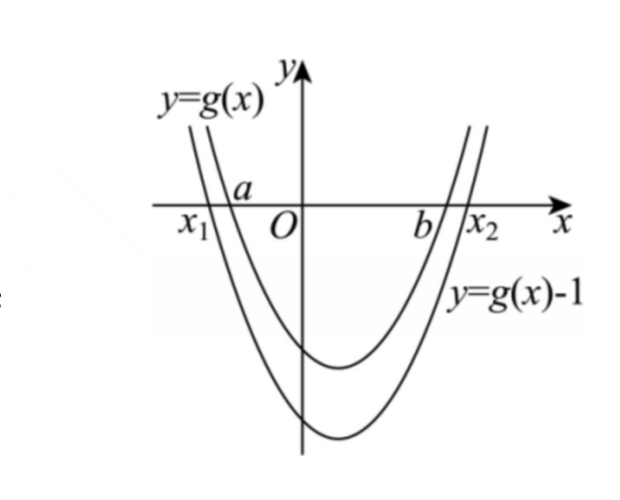
\includegraphics[width=0.20\textwidth]{figures/gao103_q16.png}
\end{center}
\step{由图像得 $x_1<a<b<x_2$．故选 $B$.}
\solend

\fi

\end{enumerate}

\bigsec{三、解答题}

\begin{enumerate}
\setcounter{enumi}{16}

\item 已知集合 $A=\{x\mid-3\leqslant x\leqslant1\}$，$B=\{x\mid a-2<x<a+2,a\in\R\}$.

（1）当 $a=1$ 时，求 $A\cap B$、$A\cup B$；

（2）若 $B\subseteq\overline A$，求 $a$ 的取值范围.

\ansspace*[8]

\ifanswer
\solbegin
\stepm{（1）}{当 $a=1$ 时，$B=\{x\mid-1<x<3\}$，又因为 $A=\{x\mid-3\leqslant x\leqslant1\}$，}
\step{所以 $A\cap B=\{x\mid-1<x\leqslant1\}$，$A\cup B=\{x\mid-3\leqslant x<3\}$；}
\stepm{（2）}{由 $A=\{x\mid-3\leqslant x\leqslant1\}$，得 $\overline A=\{x\mid x<-3\text{ 或 }x>1\}$，}
\step{若 $B\subseteq\overline A$，易得 $B=\{x\mid a-2<x<a+2,a\in\R\}\neq\varnothing$，}
\step{所以 $a+2\leqslant-3$ 或 $a-2\geqslant1$，解得 $a\leqslant-5$ 或 $a\geqslant3$，}
\step{综上所述，实数 $a$ 的取值范围是 $(-\infty,-5]\cup[3,+\infty)$.}
\solend

\fi

\item （1）解不等式 $\lvert 1-2x\rvert>x$；

（2）已知 $a$、$b$ 都是有理数，满足 $a+b\sqrt5=0$，请用反证法证明：$a=b=0$.

\ansspace*[10]

\ifanswer
\solbegin
\stepm{（1）}{①当 $x<0$ 时，左边非负，右边为负，不等式显然成立；}
\step{②当 $x\geqslant0$ 时，两边平方，$(1-2x)^2>x^2\Rightarrow3x^2-4x+1>0$}
\step{$\Rightarrow(3x-1)(x-1)>0$，解得 $x<\dfrac13$ 或 $x>1$，结合 $x\geqslant0$，}
\step{得 $0\leqslant x<\dfrac13$ 或 $x>1$；}
\step{综上，不等式解集为 $\left(-\infty,\dfrac13\right)\cup(1,+\infty)$.}
\stepm{（2）}{假设 $a,b$ 至少有一个不为零，}
\step{当 $a,b$ 中有一个为零一个不为零时，不妨设 $\begin{cases}a\neq0\\ b=0\end{cases}$，}
\step{则 $a+b\sqrt5=0\Rightarrow a=0$ 矛盾，舍；}
\step{当 $\begin{cases}a\neq0\\ b\neq0\end{cases}$ 时，$a+b\sqrt5=0\Rightarrow\sqrt5=-\dfrac ab\in\Q$，矛盾，舍，}
\step{综上假设不成立，所以 $a=b=0$.}
\solend

\fi

\item 某物流公司为了扩大业务量，计划建造一间高为 6 米，底面积为 24 平方米，且背面靠
墙的长方形形状的仓库。仓库的背面靠墙，无须建造费用，因此甲工程队给出的报价为：
仓库前面新建墙体每平方米 400 元，左右两面新建墙体每平方米 300 元，屋顶和地面以及
其他共计 28800 元.

（1）设仓库前面墙体的长为 $x$ 米 $(x>0)$，甲工程队的整体报价为 $y$ 元。若该物流公司计
划投入的改造资金不超过 60000 元，求前面墙体长 $x$ 的取值范围.

（2）在（1）的条件下，当仓库前面墙体的长度为多少时，甲工程队的整体
报价最低？

\begin{center}
% 原图第 7 页题干仓库示意图直接裁取（原卷排于题干右侧），已去粉色水印转灰度。
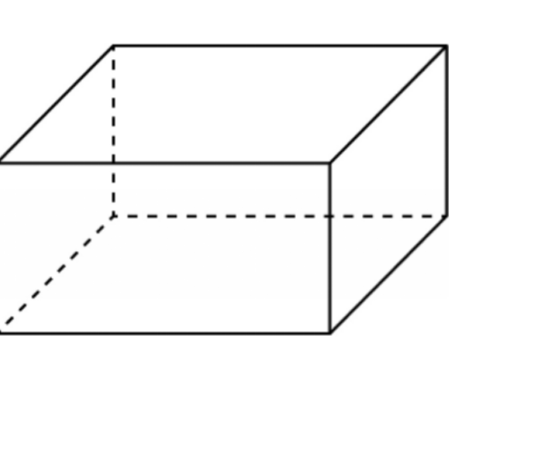
\includegraphics[width=0.17\textwidth]{figures/gao103_q19.png}
\end{center}

\ansspace*[12]

\ifanswer
\solbegin
\stepm{（1）}{甲队整体报价为 $y=400\times6x+2\times300\times6\times\dfrac{24}{x}+28800$}
\step{$=2400x+\dfrac{86400}{x}+28800$ 元，}
\step{要求 $y\leqslant60000$，即 $2400x+\dfrac{86400}{x}+28800\leqslant60000$，}
\step{化简得 $x+\dfrac{36}{x}\leqslant13$，}
\step{由于 $x>0$，则不等式化为 $x^2-13x+36\leqslant0$，}
\step{即 $(x-4)(x-9)\leqslant0$，解得 $4\leqslant x\leqslant9$，}
\step{所以前面墙体长 $x$ 的取值范围为 $[4,9]$；}
\stepm{（2）}{甲队整体报价为 $y=2400x+\dfrac{86400}{x}$}
\step{$\geqslant2\sqrt{2400x\times\dfrac{86400}{x}}+28800=57600$，}
\step{当且仅当 $2400x=\dfrac{86400}{x}$，即 $x^2=36$，}
\step{解得 $x=6$（满足 $4\leqslant x\leqslant9$）时取等号，}
\step{所以当仓库前面墙体的长度为 6 米时，甲工程队的整体报价最低，}
\step{为 57600 元.}
\solend

\fi

\item 已知函数 $f(x)=ax^2-10x+4b$.

（1）当 $a=1$，$b=4$ 时，解不等式 $f(x)\geqslant0$；

（2）若关于 $x$ 的不等式 $f(x)<0$ 的解集为 $(a,b)$，求实数 $a$、$b$ 的值；

（3）若 1 是 $f(x)$ 的零点，且 $a>0$，$b>0$，问当 $a$、$b$ 取何值时，$\dfrac1a+\dfrac1b$ 的值最小？最
小值是多少？

\ansspace*[12]

\ifanswer
\solbegin
\stepm{（1）}{将 $a=1$，$b=4$ 代入得 $f(x)=x^2-10x+16\geqslant0$，解得 $x\geqslant8$ 或 $x\leqslant2$，}
\step{所以不等式的解集为 $\{x\mid x\geqslant8\text{ 或 }x\leqslant2\}$；}
\stepm{（2）}{由题意得 $a$、$b$ 是 $ax^2-10x+4b=0$ 两根，且 $a<b$，$a>0$，}
\step{由韦达定理得 $\begin{cases}a+b=\dfrac{10}{a}\\ a\cdot b=\dfrac{4b}{a}\end{cases}$，解得 $\begin{cases}a=2\\ b=3\end{cases}$，即实数 $a$、$b$ 的值分别为 2，3；}
\stepm{（3）}{由 1 是 $f(x)$ 的零点，得 $f(1)=a-10+4b=0$，得 $a+4b=10$，}
\step{因为 $a>0$，$b>0$，}
\step{所以 $\dfrac1a+\dfrac1b=\dfrac1{10}\left(\dfrac1a+\dfrac1b\right)(a+4b)=\dfrac1{10}\left(1+4+\dfrac{4b}{a}+\dfrac ab\right)$}
\step{$\geqslant\dfrac1{10}\left(5+2\sqrt{\dfrac{4b}{a}\cdot\dfrac ab}\right)=\dfrac9{10}$，}
\step{当且仅当 $\dfrac{4b}{a}=\dfrac ab$，即 $a=\dfrac{10}3$,$b=\dfrac53$ 时取等号，}
\step{所以 $\dfrac1a+\dfrac1b$ 取最小值，且最小值为 $\dfrac9{10}$.}
\solend

\fi

\item 已知集合 $A$ 为非空集合，定义 $S=\{x\mid x=a+b,a,b\in A\}$，
$T=\{x\mid x=\lvert a-b\rvert,a,b\in A\}$.

（1）若集合 $A=\{1,3\}$，直接写出集合 $S$、$T$ (无需写计算过程)；

（2）若集合 $A=\{x_1,x_2,x_3,x_4\},x_1<x_2<x_3<x_4$，且 $T=A$，求证：$x_1+x_4=x_2+x_3$；

（3）若集合 $A=\{x\mid0\leqslant x\leqslant2026,x\in\N\}$,$S\cap T=\varnothing$．记 $\lvert A\rvert$ 为集合 $A$ 中元素的个数，求
$\lvert A\rvert$ 的最大值.

\ansspace*[16]

\ifanswer
\solbegin
\stepm{（1）}{$S=\{2,4,6\}$,$T=\{0,2\}$；}
\stepm{（2）}{集合 $T$ 中最小的元素为 0，因为 $T=A$，且 $x_1<x_2<x_3<x_4$，所以 $x_1=0$，}
\step{所以集合 $T$ 中元素为 $x_2-x_1=x_2$,$x_3-x_1=x_3$,$x_4-x_1=x_4$，}
\step{以及 $x_3-x_2$,$x_4-x_2$,$x_4-x_3$ 均属于 $A$，}
\step{因为 $x_1=0<x_3-x_2<x_4-x_2<x_4$，所以 $x_3$ 即 $x_4-x_2=x_3-x_1$，}
\step{即 $x_1+x_4=x_2+x_3$；}
\stepm{（3）}{设 $A=\{a_1,a_2,a_3,\cdots,a_k\}$ 满足题意，其中 $a_1<a_2<\cdots<a_k$，}
\step{则 $2a_1<a_1+a_2<\cdots<a_1+a_k<a_2+a_k<a_3+a_k<\cdots<a_{k-1}+a_k<2a_k$，}
\step{所以 $\lvert S\cup T\rvert\leqslant2k+1$，所以 $3k-1\leqslant2a_k+1\leqslant4053(k\in\N^*)$，}
\step{所以 $k\leqslant1351$，}
\step{实际上当 $A=\{676,677,\cdots,2026\}$ 时满足题意，}
\step{证明如下：设 $A=\{m,m+1,m+2,\cdots,2026\},m\in N$，}
\step{设 $S=\{2m,2m+1,2m+2,\cdots,4052\}$,$T=\{0,1,2,\cdots,2026-m\}$，}
\step{由题意得 $2026-m<2m$，即 $m>675\dfrac13$，}
\step{故 $m$ 的最小值是 676，于是当 $m=676$,$A$ 中的元素最多，}
\step{即 $A=\{676,677,\cdots,2026\}$ 时满足题意，}
\step{综上所述，集合 $A$ 中元素的个数的最大值是 1351.}
\solend

\fi

\end{enumerate}

\end{document}
"
% 紧凑版：xelatex "\def\iscompact{1}% 高一103_市北中学_10月月考.tex
%   —— 高一上数学“2026-2027 年市北中学高一上 10 月月考”（试卷版/答案版）
% 试卷版：xelatex 高一103_市北中学_10月月考.tex
% 答案版：xelatex "\def\isanswer{1}% 高一103_市北中学_10月月考.tex
%   —— 高一上数学“2026-2027 年市北中学高一上 10 月月考”（试卷版/答案版）
% 试卷版：xelatex 高一103_市北中学_10月月考.tex
% 答案版：xelatex "\def\isanswer{1}% 高一103_市北中学_10月月考.tex
%   —— 高一上数学“2026-2027 年市北中学高一上 10 月月考”（试卷版/答案版）
% 试卷版：xelatex 高一103_市北中学_10月月考.tex
% 答案版：xelatex "\def\isanswer{1}\input{高一103_市北中学_10月月考.tex}"
% 紧凑版：xelatex "\def\iscompact{1}\input{高一103_市北中学_10月月考.tex}"
%
% 原始材料：微信公众号“魔都数学加油站”文章，作者破晓，2026-11-01 21:56 发布；
% 连载“27学年高一103”，原文标题“27学年高一103——2026-2027年上海市市北中学高一上10月月考”；
% 原文链接：https://mp.weixin.qq.com/s/iBvF4eKw66F-kS6xLmDpBA。
% 正文为 10 张 PNG 页（第 1、3、5、6、7、10 页 2560×3620，其余 4762×6735），题目下印有【解析】，为讲评版。
% 题目、解析均据原图转录；卷面水印及公众号页脚未录入。
%
% 卷首标题：原卷印作“2026-2027 年市北中学高一上 10 月月考”（公众号标题中的“上海市”“高一上”
% 卷面标题行没有或已含，本稿照卷面），年份区间按全稿惯例排 en dash；原卷未印副标题，本稿按题目
% 内容标为“集合与常用逻辑用语、不等式”。
%
% 与原卷的排版差异：
%   ① 原文从第 3 题起，填空题编号为 3—12、选择题为 13—16、解答题为 17—21，本稿保留原题号；
%   ② 原卷每题下直接印【解析】，本稿按全稿惯例将解析置于答案版；选择题括号内未印答案，另由
%      解析末句“故选 X”给出；
%   ③ 原卷未印副标题，本稿按“知识模块”口径补出；
%   ④ 原卷填空横线按全稿惯例排为 \blankline[4.4em]；解答题按惯例加 \ansspace；选择题括号排
%      \mbox{（\quad）}；
%   ⑤ 原卷数集排斜体 $R$／$Q$（第 18 题解析 $Q$ 排粗体），按全稿惯例改 $\R$／$\Q$；
%   ⑥ 第 14 题四个文氏图选项按原图形状用 TikZ 重排；第 16、19 两题的插图裁自原图
%      （去粉色水印转灰度），第 19 题图属题干（三版都出），第 16 题图属解析（仅答案版显示）。
%
% 原卷存疑／笔误（均照录加注）：
%   第 9 题解析“故 $a+b=3b+b<0$”（$a=3b$ 代入应为 $4b$，原卷写作 $3b+b$，数值相同）；
%   第 21 题 (2) 解析“所以 $x_3$ 即 $x_4-x_2=x_3-x_1$”表述含糊（意为 $x_4-x_2$ 恰为 $T$ 中
%   介于 $x_2$ 与 $x_4$ 之间的元素 $x_3-x_1$）；
%   第 21 题 (3) 解析“所以 $|S\cup T|\leqslant2k+1$”（按上下文应为 $2a_k+1$，与后半句
%   $3k-1\leqslant2a_k+1$ 呼应），照录。
%
% 行数核对：逐题数 \step/\stepm 条数，合计 119 条（Q3：2；Q4：2；Q5：5；Q6：3；Q8：3；
% Q9：7；Q10：5；Q11：8；Q12：7；Q13：6；Q14：5；Q15：6；Q16：4；Q17：6；Q18：10；
% Q19：13；Q20：10；Q21：17），与原卷印刷行逐题相等。第 7 题只印【答案】，提 \ans{}，
% 不计入 \step 账。
%
\documentclass[a4paper,11pt]{article}
\usepackage{common}

\begin{document}

\examtitlest[3]{2026--2027 年市北中学高一上 10 月月考}{集合与常用逻辑用语、不等式}

\bigsec{一、填空题}

\begin{enumerate}
\setcounter{enumi}{2}

\item 已知实数 $x$ 满足 $\dfrac{7-x}{x+4}>0$，则 $x$ 的取值范围是\blankline[4.4em].

\ifanswer
\solbegin
\step{不等式 $\dfrac{7-x}{x+4}>0$ 可化为 $\dfrac{x-7}{x+4}<0$，等价于 $(x-7)(x+4)<0$，}
\step{解得 $-4<x<7$，所以 $x$ 的取值范围是 $\{x\mid-4<x<7\}$.}
\solend

\fi

\item 已知 $x_1$、$x_2$ 为方程 $2x^2+6x+3=0$ 的两个实数根，则 $\dfrac1{x_1}+\dfrac1{x_2}=$\blankline[4.4em].

\ifanswer
\solbegin
\step{由根与系数的关系得 $x_1+x_2=-\dfrac62=-3$，$x_1x_2=\dfrac32$，}
\step{则 $\dfrac1{x_1}+\dfrac1{x_2}=\dfrac{x_1+x_2}{x_1x_2}=-2$.}
\solend

\fi

\item 已知 $y=\lvert x-2\rvert+\lvert x-5\rvert$，$x\in\R$，则 $y$ 的最小值为\blankline[4.4em].

\ifanswer
\solbegin
\step{$y=\lvert x-2\rvert+\lvert x-5\rvert=\begin{cases}7-2x, & x<2\\ 3, & 2\leqslant x\leqslant5\\ 2x-7, & x>5\end{cases}$，}
\step{当 $x<2$ 时，$y>7-2\times2=3$；}
\step{当 $2\leqslant x\leqslant5$ 时，$y=3$；}
\step{当 $x>5$ 时，$y>2\times5-7=3$.}
\step{综上所述，$y$ 的最小值为 3.}
\solend

\fi

\item 对任意实数 $x$，等式 $ax^4+bx^3+cx^2+dx+e=x(x-2)(x^2+3)$ 恒成立，则
$b+c+d=$\blankline[4.4em].

\ifanswer
\solbegin
\step{因为 $ax^4+bx^3+cx^2+dx+e=x(x-2)(x^2+3)=(x^2-2x)(x^2+3)$}
\step{$=x^4-2x^3+3x^2-6x$，所以 $a=1$，$b=-2$，$c=3$，$d=-6$，$e=0$，}
\step{所以 $b+c+d=-2+3-6=-5$.}
\solend

\fi

\item 命题：“存在 $x\in(1,+\infty)$，使得 $ax^2+bx+c<0$”的否定形式是\blankline[4.4em].

\ifanswer
\ans{对于任意的 $x\in(1,+\infty)$，都有 $ax^2+bx+c\geqslant0$}
\fi

\item 已知集合 $A=\{x\mid mx^2-2x+1=0,x\in\R\}$ 有且仅有两个子集，则实数 $m=$\blankline[4.4em].

\ifanswer
\solbegin
\step{①当 $m=0$ 时，方程为 $-2x+1=0$，解得 $x=\dfrac12$，满足 $A=\left\{\dfrac12\right\}$ 仅有两个子集；}
\step{②当 $m\neq0$ 时，方程有两个相等实根，所以 $\Delta=4-4m=0$，解得 $m=1$；}
\step{所以实数 $m$ 的值为 0 或 1.}
\solend

\fi

\item 设 $a$、$b\in\R$，已知关于 $x$ 的不等式 $(a+b)x+(b-3a)<0$ 的解集为 $(2,+\infty)$，则不等式
$(a-2b)x+5b-a>0$ 的解集为\blankline[4.4em].

\ifanswer
\solbegin
\step{关于 $x$ 的不等式 $(a+b)x+(b-3a)<0$ 的解集为 $(2,+\infty)$，}
\step{得 $x=2$ 是 $(a+b)x+(b-3a)=0$ 的解，且 $a+b<0$，}
\step{所以 $2(a+b)+(b-3a)=0$，化简得 $a=3b$，故 $a+b=3b+b<0$，即 $b<0$，}
\step{将 $a=3b$ 代入 $(a-2b)x+5b-a>0$，}
\step{得不等式 $(a-2b)x+5b-a>0$ 即 $b(x+2)>0$，}
\step{两边都除以 $b$，得 $x+2<0$，解得 $x<-2$，}
\step{所以不等式 $(a-2b)x+5b-a>0$ 的解集为 $(-\infty,-2)$.}
\solend

\fi

\item 已知不等式 $\lvert x-a\rvert<1$ 成立的充分不必要条件是 $\dfrac12<x<\dfrac32$，则实数 $a$ 的取值范围
是\blankline[4.4em].

\ifanswer
\solbegin
\step{$\lvert x-a\rvert<1$，解得 $a-1<x<1+a$，}
\step{所以 $a-1<x<1+a$ 成立的充分不必要条件是 $\dfrac12<x<\dfrac32$，}
\step{故 $\left\{x\left|\dfrac12<x<\dfrac32\right.\right\}$ 是 $\{x\mid a-1<x<1+a\}$ 的真子集，}
\step{所以 $a-1\leqslant\dfrac12$ 且 $1+a\geqslant\dfrac32$（等号不同时成立），解得 $\dfrac12\leqslant a\leqslant\dfrac32$，}
\step{故实数 $a$ 的取值范围是 $\left[\dfrac12,\dfrac32\right]$.}
\solend

\fi

\item 定义 $A\nabla B=\left\{z\,\middle|\,z=xy+\dfrac xy,x\in A,y\in B\right\}$，设集合 $A=\{0,2\}$，$B=\{1,2\}$，$C=\{1\}$，
则集合 $(A\nabla B)\nabla C=$\blankline[4.4em].

\ifanswer
\solbegin
\step{当 $x=0$，$y=1$ 或 2 时，$z=xy+\dfrac xy=0$；}
\step{当 $x=2$，$y=1$ 时，$z=xy+\dfrac xy=4$；}
\step{当 $x=2$，$y=2$ 时，$z=xy+\dfrac xy=5$；}
\step{所以 $A\nabla B=\{0,4,5\}$；}
\step{当 $x=0$，$y=1$ 时，$z=xy+\dfrac xy=0$；}
\step{当 $x=4$，$y=1$ 时，$z=xy+\dfrac xy=8$；}
\step{当 $x=5$，$y=1$ 时，$z=xy+\dfrac xy=10$；}
\step{所以 $(A\nabla B)\nabla C=\{0,8,10\}$.}
\solend

\fi

\item 集合 $M=\{66,-11,23,10,911,-1,-18,100,0,\pi\}$ 有 10 个元素，设 $M$ 的所有非空子集为
$M_i\,(i=1,2,\cdots,1023)$，每一个 $M_i$ 中所有元素乘积为 $m_i\,(i=1,2,\cdots,1023)$，则
$m_1+m_2+m_3+\cdots+m_{1023}=$\blankline[4.4em].

\ifanswer
\solbegin
\step{因为 $M$ 的所有非空子集为 $M_i\,(i=1,2,\cdots,1023)$，这 1023 个子集分成以下几种情况：}
\step{①含 0 的子集有 512 个，这些子集均满足 $m_i=0$；}
\step{②不含 0，含 $-1$ 且还含有其它元素的子集有 255 个，}
\step{③不含 0，不含 $-1$ 但含有其它元素的子集有 255 个，}
\step{④只含 $-1$ 的子集一个 $\{-1\}$，满足 $m_i=-1$；}
\step{其中②③中的集合是一一对应的，且满足 $m_i$ 对应成相反数，}
\step{故 $m_1+m_2+m_3+\cdots+m_{1023}=512\times0+255\times0-1=-1$.}
\solend

\fi

\end{enumerate}

\bigsec{二、选择题}

\begin{enumerate}
\setcounter{enumi}{12}

\item 下列说法中，正确说法的个数是\mbox{（\quad）}

①联合国安理会常任理事国能组成一个集合；

②市北中学很喜欢足球的同学能组成一个集合；

③实数 $1,0,5,\dfrac12,\dfrac32,\dfrac64,\sqrt{\dfrac14}$ 组成的集合中有 6 个元素.

\keepwithprev
A. $0$\qquad\qquad B. $1$\qquad\qquad C. $2$\qquad\qquad D. $3$.

\ifanswer
\solbegin
\step{对于①，“联合国安理会常任理事国”满足集合的定义，故①正确；}
\step{对于②，“很喜欢”不满足集合的确定性，}
\step{市北中学很喜欢足球的同学不能组成一个集合，故②错误；}
\step{对于③，$\dfrac64=\dfrac32$，$\sqrt{\dfrac14}=\dfrac12$，由集合的元素互异性，集合中共有 5 个元素，}
\step{故③错误.}
\step{所以正确说法的个数是 1 个．故选 $B$.}
\solend

\fi

\item 已知全集 $U=\R$，集合 $A=\left\{x\,\middle|\,\dfrac{2x-8}{x-5}\leqslant1,x\in\N\right\}$，集合 $B=\{x\mid x^2-7x+12\leqslant0\}$，则
正确表示集合 $A$ 与集合 $B$ 关系的文氏图是\mbox{（\quad）}

\keepwithprev
\begin{center}
% 原卷四个文氏图选项按原图形状用 TikZ 重排。
\begin{tabular}{c@{\qquad\qquad}c}
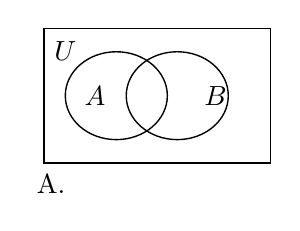
\begin{tikzpicture}[scale=0.9,line width=0.5pt]
\draw (0,0) rectangle (3.2,1.9);
\draw (1.02,0.95) ellipse (0.72 and 0.62);
\draw (1.88,0.95) ellipse (0.72 and 0.62);
\node at (0.72,0.95) {$A$};
\node at (2.42,0.95) {$B$};
\node at (0.3,1.58) {$U$};
\node[anchor=north] at (0.1,-0.03) {A.};
\end{tikzpicture}
&
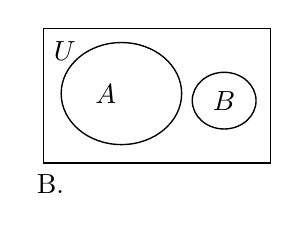
\begin{tikzpicture}[scale=0.9,line width=0.5pt]
\draw (0,0) rectangle (3.2,1.9);
\draw (1.1,0.98) ellipse (0.85 and 0.72);
\draw (2.55,0.88) ellipse (0.45 and 0.4);
\node at (0.88,0.98) {$A$};
\node at (2.55,0.88) {$B$};
\node at (0.3,1.58) {$U$};
\node[anchor=north] at (0.1,-0.03) {B.};
\end{tikzpicture}
\\[10pt]
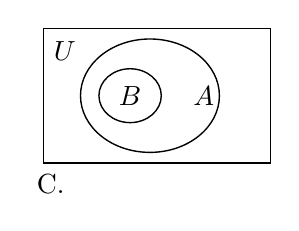
\begin{tikzpicture}[scale=0.9,line width=0.5pt]
\draw (0,0) rectangle (3.2,1.9);
\draw (1.5,0.95) ellipse (0.98 and 0.8);
\draw (1.22,0.95) ellipse (0.44 and 0.38);
\node at (1.22,0.95) {$B$};
\node at (2.26,0.95) {$A$};
\node at (0.3,1.58) {$U$};
\node[anchor=north] at (0.1,-0.03) {C.};
\end{tikzpicture}
&
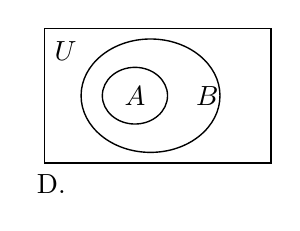
\begin{tikzpicture}[scale=0.9,line width=0.5pt]
\draw (0,0) rectangle (3.2,1.9);
\draw (1.5,0.95) ellipse (0.98 and 0.8);
\draw (1.28,0.95) ellipse (0.46 and 0.4);
\node at (1.28,0.95) {$A$};
\node at (2.3,0.95) {$B$};
\node at (0.3,1.58) {$U$};
\node[anchor=north] at (0.1,-0.03) {D.};
\end{tikzpicture}
\\
\end{tabular}
\end{center}

\ifanswer
\solbegin
\step{$\dfrac{2x-8}{x-5}\leqslant1\Rightarrow\dfrac{2x-8}{x-5}-1\leqslant0\Rightarrow\dfrac{x-3}{x-5}\leqslant0$，等价于 $\begin{cases}(x-3)(x-5)\leqslant0\\ x-5\neq0\end{cases}$，}
\step{解得 $3\leqslant x<5$，因为 $x\in\N$，所以 $A=\{3,4\}$，}
\step{解不等式 $x^2-7x+12\leqslant0$ 得 $B=\{x\mid3\leqslant x\leqslant4\}$，}
\step{集合 $A$ 中的元素 3，4 都属于集合 $B$，且 $B$ 中存在无数实数不属于 $A$，}
\step{所以 $A$ 是 $B$ 的真子集，$A$ 在 $B$ 内部．故选 $D$.}
\solend

\fi

\item 已知 $a$、$b$、$c\in\R$，则下列命题中真命题的个数是\mbox{（\quad）}

①若 $ac^2>bc^2$，则 $a>b$；②若 $\lvert a-2\rvert>\lvert b-2\rvert$，则 $(a-2)^2>(b-2)^2$；

③若 $a>b>c>0$，则 $\dfrac ab>\dfrac{a+c}{b+c}$；④若 $a>0$，$b>0$，$a+b>4$，$ab>4$，则 $a>2$，$b>2$.

\keepwithprev
A. $1$\qquad\qquad B. $2$\qquad\qquad C. $3$\qquad\qquad D. $4$

\ifanswer
\solbegin
\step{①若 $ac^2>bc^2$，则 $c^2>0$，则 $a>b$；所以①正确；}
\step{②若 $\lvert a-2\rvert>\lvert b-2\rvert$，则 $(a-2)^2>(b-2)^2$；满足不等式的基本性质，所以②正确；}
\step{③若 $a>b>c>0$，则 $\dfrac ab>\dfrac{a+c}{b+c}$；所以③正确；}
\step{④若 $a>0$，$b>0$，$a+b>4$，$ab>4$，则 $a>2$，$b>2$.}
\step{反例 $a=10$，$b=0.5$，满足条件，推不出结论，所以④不正确；}
\step{故选 $C$.}
\solend

\fi

\item 已知实数 $a<b$，关于 $x$ 的不等式 $x^2-(a+b)x+ab-1<0$ 的解集为 $(x_1,x_2)$，则实数
$a$、$b$、$x_1$、$x_2$ 从小到大的排列是\mbox{（\quad）}

\keepwithprev
A. $x_1<a<x_2<b$\qquad B. $x_1<a<b<x_2$\qquad C. $a<x_1<b<x_2$\qquad D. $a<x_1<x_2<b$

\ifanswer
\solbegin
\step{已知实数 $a<b$，关于 $x$ 的不等式 $x^2-(a+b)x+ab-1<0$ 的解集为 $(x_1,x_2)$，}
\step{因为 $x^2-(a+b)x+ab=(x-a)(x-b)$.}
\step{设函数 $g(x)=(x-a)(x-b)$，作函数 $g(x)$、$g(x)-1$ 的图象如下：}
\begin{center}
% 原图第 6 页解析插图直接裁取（原卷排于解析行右侧），已去粉色水印转灰度。
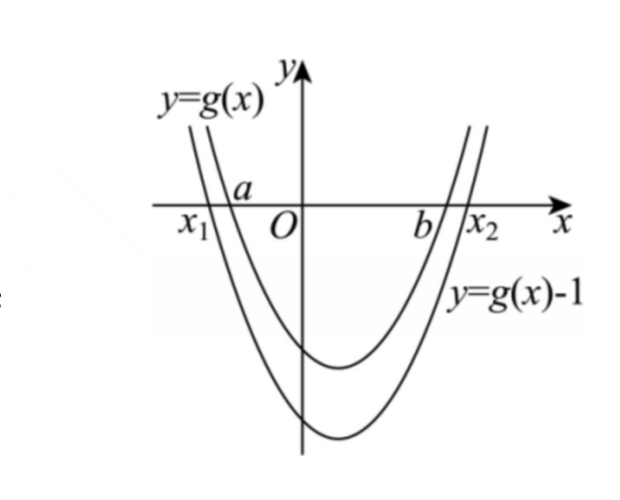
\includegraphics[width=0.20\textwidth]{figures/gao103_q16.png}
\end{center}
\step{由图像得 $x_1<a<b<x_2$．故选 $B$.}
\solend

\fi

\end{enumerate}

\bigsec{三、解答题}

\begin{enumerate}
\setcounter{enumi}{16}

\item 已知集合 $A=\{x\mid-3\leqslant x\leqslant1\}$，$B=\{x\mid a-2<x<a+2,a\in\R\}$.

（1）当 $a=1$ 时，求 $A\cap B$、$A\cup B$；

（2）若 $B\subseteq\overline A$，求 $a$ 的取值范围.

\ansspace*[8]

\ifanswer
\solbegin
\stepm{（1）}{当 $a=1$ 时，$B=\{x\mid-1<x<3\}$，又因为 $A=\{x\mid-3\leqslant x\leqslant1\}$，}
\step{所以 $A\cap B=\{x\mid-1<x\leqslant1\}$，$A\cup B=\{x\mid-3\leqslant x<3\}$；}
\stepm{（2）}{由 $A=\{x\mid-3\leqslant x\leqslant1\}$，得 $\overline A=\{x\mid x<-3\text{ 或 }x>1\}$，}
\step{若 $B\subseteq\overline A$，易得 $B=\{x\mid a-2<x<a+2,a\in\R\}\neq\varnothing$，}
\step{所以 $a+2\leqslant-3$ 或 $a-2\geqslant1$，解得 $a\leqslant-5$ 或 $a\geqslant3$，}
\step{综上所述，实数 $a$ 的取值范围是 $(-\infty,-5]\cup[3,+\infty)$.}
\solend

\fi

\item （1）解不等式 $\lvert 1-2x\rvert>x$；

（2）已知 $a$、$b$ 都是有理数，满足 $a+b\sqrt5=0$，请用反证法证明：$a=b=0$.

\ansspace*[10]

\ifanswer
\solbegin
\stepm{（1）}{①当 $x<0$ 时，左边非负，右边为负，不等式显然成立；}
\step{②当 $x\geqslant0$ 时，两边平方，$(1-2x)^2>x^2\Rightarrow3x^2-4x+1>0$}
\step{$\Rightarrow(3x-1)(x-1)>0$，解得 $x<\dfrac13$ 或 $x>1$，结合 $x\geqslant0$，}
\step{得 $0\leqslant x<\dfrac13$ 或 $x>1$；}
\step{综上，不等式解集为 $\left(-\infty,\dfrac13\right)\cup(1,+\infty)$.}
\stepm{（2）}{假设 $a,b$ 至少有一个不为零，}
\step{当 $a,b$ 中有一个为零一个不为零时，不妨设 $\begin{cases}a\neq0\\ b=0\end{cases}$，}
\step{则 $a+b\sqrt5=0\Rightarrow a=0$ 矛盾，舍；}
\step{当 $\begin{cases}a\neq0\\ b\neq0\end{cases}$ 时，$a+b\sqrt5=0\Rightarrow\sqrt5=-\dfrac ab\in\Q$，矛盾，舍，}
\step{综上假设不成立，所以 $a=b=0$.}
\solend

\fi

\item 某物流公司为了扩大业务量，计划建造一间高为 6 米，底面积为 24 平方米，且背面靠
墙的长方形形状的仓库。仓库的背面靠墙，无须建造费用，因此甲工程队给出的报价为：
仓库前面新建墙体每平方米 400 元，左右两面新建墙体每平方米 300 元，屋顶和地面以及
其他共计 28800 元.

（1）设仓库前面墙体的长为 $x$ 米 $(x>0)$，甲工程队的整体报价为 $y$ 元。若该物流公司计
划投入的改造资金不超过 60000 元，求前面墙体长 $x$ 的取值范围.

（2）在（1）的条件下，当仓库前面墙体的长度为多少时，甲工程队的整体
报价最低？

\begin{center}
% 原图第 7 页题干仓库示意图直接裁取（原卷排于题干右侧），已去粉色水印转灰度。
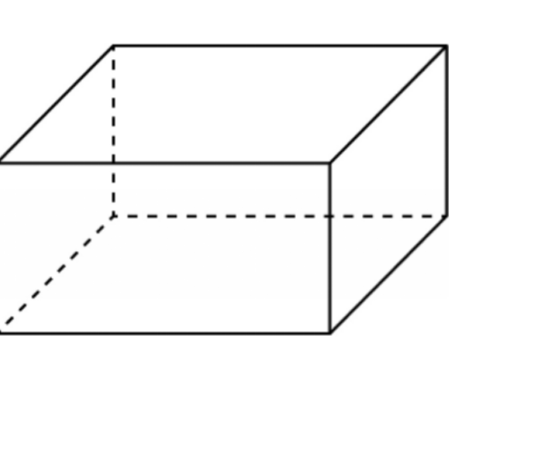
\includegraphics[width=0.17\textwidth]{figures/gao103_q19.png}
\end{center}

\ansspace*[12]

\ifanswer
\solbegin
\stepm{（1）}{甲队整体报价为 $y=400\times6x+2\times300\times6\times\dfrac{24}{x}+28800$}
\step{$=2400x+\dfrac{86400}{x}+28800$ 元，}
\step{要求 $y\leqslant60000$，即 $2400x+\dfrac{86400}{x}+28800\leqslant60000$，}
\step{化简得 $x+\dfrac{36}{x}\leqslant13$，}
\step{由于 $x>0$，则不等式化为 $x^2-13x+36\leqslant0$，}
\step{即 $(x-4)(x-9)\leqslant0$，解得 $4\leqslant x\leqslant9$，}
\step{所以前面墙体长 $x$ 的取值范围为 $[4,9]$；}
\stepm{（2）}{甲队整体报价为 $y=2400x+\dfrac{86400}{x}$}
\step{$\geqslant2\sqrt{2400x\times\dfrac{86400}{x}}+28800=57600$，}
\step{当且仅当 $2400x=\dfrac{86400}{x}$，即 $x^2=36$，}
\step{解得 $x=6$（满足 $4\leqslant x\leqslant9$）时取等号，}
\step{所以当仓库前面墙体的长度为 6 米时，甲工程队的整体报价最低，}
\step{为 57600 元.}
\solend

\fi

\item 已知函数 $f(x)=ax^2-10x+4b$.

（1）当 $a=1$，$b=4$ 时，解不等式 $f(x)\geqslant0$；

（2）若关于 $x$ 的不等式 $f(x)<0$ 的解集为 $(a,b)$，求实数 $a$、$b$ 的值；

（3）若 1 是 $f(x)$ 的零点，且 $a>0$，$b>0$，问当 $a$、$b$ 取何值时，$\dfrac1a+\dfrac1b$ 的值最小？最
小值是多少？

\ansspace*[12]

\ifanswer
\solbegin
\stepm{（1）}{将 $a=1$，$b=4$ 代入得 $f(x)=x^2-10x+16\geqslant0$，解得 $x\geqslant8$ 或 $x\leqslant2$，}
\step{所以不等式的解集为 $\{x\mid x\geqslant8\text{ 或 }x\leqslant2\}$；}
\stepm{（2）}{由题意得 $a$、$b$ 是 $ax^2-10x+4b=0$ 两根，且 $a<b$，$a>0$，}
\step{由韦达定理得 $\begin{cases}a+b=\dfrac{10}{a}\\ a\cdot b=\dfrac{4b}{a}\end{cases}$，解得 $\begin{cases}a=2\\ b=3\end{cases}$，即实数 $a$、$b$ 的值分别为 2，3；}
\stepm{（3）}{由 1 是 $f(x)$ 的零点，得 $f(1)=a-10+4b=0$，得 $a+4b=10$，}
\step{因为 $a>0$，$b>0$，}
\step{所以 $\dfrac1a+\dfrac1b=\dfrac1{10}\left(\dfrac1a+\dfrac1b\right)(a+4b)=\dfrac1{10}\left(1+4+\dfrac{4b}{a}+\dfrac ab\right)$}
\step{$\geqslant\dfrac1{10}\left(5+2\sqrt{\dfrac{4b}{a}\cdot\dfrac ab}\right)=\dfrac9{10}$，}
\step{当且仅当 $\dfrac{4b}{a}=\dfrac ab$，即 $a=\dfrac{10}3$,$b=\dfrac53$ 时取等号，}
\step{所以 $\dfrac1a+\dfrac1b$ 取最小值，且最小值为 $\dfrac9{10}$.}
\solend

\fi

\item 已知集合 $A$ 为非空集合，定义 $S=\{x\mid x=a+b,a,b\in A\}$，
$T=\{x\mid x=\lvert a-b\rvert,a,b\in A\}$.

（1）若集合 $A=\{1,3\}$，直接写出集合 $S$、$T$ (无需写计算过程)；

（2）若集合 $A=\{x_1,x_2,x_3,x_4\},x_1<x_2<x_3<x_4$，且 $T=A$，求证：$x_1+x_4=x_2+x_3$；

（3）若集合 $A=\{x\mid0\leqslant x\leqslant2026,x\in\N\}$,$S\cap T=\varnothing$．记 $\lvert A\rvert$ 为集合 $A$ 中元素的个数，求
$\lvert A\rvert$ 的最大值.

\ansspace*[16]

\ifanswer
\solbegin
\stepm{（1）}{$S=\{2,4,6\}$,$T=\{0,2\}$；}
\stepm{（2）}{集合 $T$ 中最小的元素为 0，因为 $T=A$，且 $x_1<x_2<x_3<x_4$，所以 $x_1=0$，}
\step{所以集合 $T$ 中元素为 $x_2-x_1=x_2$,$x_3-x_1=x_3$,$x_4-x_1=x_4$，}
\step{以及 $x_3-x_2$,$x_4-x_2$,$x_4-x_3$ 均属于 $A$，}
\step{因为 $x_1=0<x_3-x_2<x_4-x_2<x_4$，所以 $x_3$ 即 $x_4-x_2=x_3-x_1$，}
\step{即 $x_1+x_4=x_2+x_3$；}
\stepm{（3）}{设 $A=\{a_1,a_2,a_3,\cdots,a_k\}$ 满足题意，其中 $a_1<a_2<\cdots<a_k$，}
\step{则 $2a_1<a_1+a_2<\cdots<a_1+a_k<a_2+a_k<a_3+a_k<\cdots<a_{k-1}+a_k<2a_k$，}
\step{所以 $\lvert S\cup T\rvert\leqslant2k+1$，所以 $3k-1\leqslant2a_k+1\leqslant4053(k\in\N^*)$，}
\step{所以 $k\leqslant1351$，}
\step{实际上当 $A=\{676,677,\cdots,2026\}$ 时满足题意，}
\step{证明如下：设 $A=\{m,m+1,m+2,\cdots,2026\},m\in N$，}
\step{设 $S=\{2m,2m+1,2m+2,\cdots,4052\}$,$T=\{0,1,2,\cdots,2026-m\}$，}
\step{由题意得 $2026-m<2m$，即 $m>675\dfrac13$，}
\step{故 $m$ 的最小值是 676，于是当 $m=676$,$A$ 中的元素最多，}
\step{即 $A=\{676,677,\cdots,2026\}$ 时满足题意，}
\step{综上所述，集合 $A$ 中元素的个数的最大值是 1351.}
\solend

\fi

\end{enumerate}

\end{document}
"
% 紧凑版：xelatex "\def\iscompact{1}% 高一103_市北中学_10月月考.tex
%   —— 高一上数学“2026-2027 年市北中学高一上 10 月月考”（试卷版/答案版）
% 试卷版：xelatex 高一103_市北中学_10月月考.tex
% 答案版：xelatex "\def\isanswer{1}\input{高一103_市北中学_10月月考.tex}"
% 紧凑版：xelatex "\def\iscompact{1}\input{高一103_市北中学_10月月考.tex}"
%
% 原始材料：微信公众号“魔都数学加油站”文章，作者破晓，2026-11-01 21:56 发布；
% 连载“27学年高一103”，原文标题“27学年高一103——2026-2027年上海市市北中学高一上10月月考”；
% 原文链接：https://mp.weixin.qq.com/s/iBvF4eKw66F-kS6xLmDpBA。
% 正文为 10 张 PNG 页（第 1、3、5、6、7、10 页 2560×3620，其余 4762×6735），题目下印有【解析】，为讲评版。
% 题目、解析均据原图转录；卷面水印及公众号页脚未录入。
%
% 卷首标题：原卷印作“2026-2027 年市北中学高一上 10 月月考”（公众号标题中的“上海市”“高一上”
% 卷面标题行没有或已含，本稿照卷面），年份区间按全稿惯例排 en dash；原卷未印副标题，本稿按题目
% 内容标为“集合与常用逻辑用语、不等式”。
%
% 与原卷的排版差异：
%   ① 原文从第 3 题起，填空题编号为 3—12、选择题为 13—16、解答题为 17—21，本稿保留原题号；
%   ② 原卷每题下直接印【解析】，本稿按全稿惯例将解析置于答案版；选择题括号内未印答案，另由
%      解析末句“故选 X”给出；
%   ③ 原卷未印副标题，本稿按“知识模块”口径补出；
%   ④ 原卷填空横线按全稿惯例排为 \blankline[4.4em]；解答题按惯例加 \ansspace；选择题括号排
%      \mbox{（\quad）}；
%   ⑤ 原卷数集排斜体 $R$／$Q$（第 18 题解析 $Q$ 排粗体），按全稿惯例改 $\R$／$\Q$；
%   ⑥ 第 14 题四个文氏图选项按原图形状用 TikZ 重排；第 16、19 两题的插图裁自原图
%      （去粉色水印转灰度），第 19 题图属题干（三版都出），第 16 题图属解析（仅答案版显示）。
%
% 原卷存疑／笔误（均照录加注）：
%   第 9 题解析“故 $a+b=3b+b<0$”（$a=3b$ 代入应为 $4b$，原卷写作 $3b+b$，数值相同）；
%   第 21 题 (2) 解析“所以 $x_3$ 即 $x_4-x_2=x_3-x_1$”表述含糊（意为 $x_4-x_2$ 恰为 $T$ 中
%   介于 $x_2$ 与 $x_4$ 之间的元素 $x_3-x_1$）；
%   第 21 题 (3) 解析“所以 $|S\cup T|\leqslant2k+1$”（按上下文应为 $2a_k+1$，与后半句
%   $3k-1\leqslant2a_k+1$ 呼应），照录。
%
% 行数核对：逐题数 \step/\stepm 条数，合计 119 条（Q3：2；Q4：2；Q5：5；Q6：3；Q8：3；
% Q9：7；Q10：5；Q11：8；Q12：7；Q13：6；Q14：5；Q15：6；Q16：4；Q17：6；Q18：10；
% Q19：13；Q20：10；Q21：17），与原卷印刷行逐题相等。第 7 题只印【答案】，提 \ans{}，
% 不计入 \step 账。
%
\documentclass[a4paper,11pt]{article}
\usepackage{common}

\begin{document}

\examtitlest[3]{2026--2027 年市北中学高一上 10 月月考}{集合与常用逻辑用语、不等式}

\bigsec{一、填空题}

\begin{enumerate}
\setcounter{enumi}{2}

\item 已知实数 $x$ 满足 $\dfrac{7-x}{x+4}>0$，则 $x$ 的取值范围是\blankline[4.4em].

\ifanswer
\solbegin
\step{不等式 $\dfrac{7-x}{x+4}>0$ 可化为 $\dfrac{x-7}{x+4}<0$，等价于 $(x-7)(x+4)<0$，}
\step{解得 $-4<x<7$，所以 $x$ 的取值范围是 $\{x\mid-4<x<7\}$.}
\solend

\fi

\item 已知 $x_1$、$x_2$ 为方程 $2x^2+6x+3=0$ 的两个实数根，则 $\dfrac1{x_1}+\dfrac1{x_2}=$\blankline[4.4em].

\ifanswer
\solbegin
\step{由根与系数的关系得 $x_1+x_2=-\dfrac62=-3$，$x_1x_2=\dfrac32$，}
\step{则 $\dfrac1{x_1}+\dfrac1{x_2}=\dfrac{x_1+x_2}{x_1x_2}=-2$.}
\solend

\fi

\item 已知 $y=\lvert x-2\rvert+\lvert x-5\rvert$，$x\in\R$，则 $y$ 的最小值为\blankline[4.4em].

\ifanswer
\solbegin
\step{$y=\lvert x-2\rvert+\lvert x-5\rvert=\begin{cases}7-2x, & x<2\\ 3, & 2\leqslant x\leqslant5\\ 2x-7, & x>5\end{cases}$，}
\step{当 $x<2$ 时，$y>7-2\times2=3$；}
\step{当 $2\leqslant x\leqslant5$ 时，$y=3$；}
\step{当 $x>5$ 时，$y>2\times5-7=3$.}
\step{综上所述，$y$ 的最小值为 3.}
\solend

\fi

\item 对任意实数 $x$，等式 $ax^4+bx^3+cx^2+dx+e=x(x-2)(x^2+3)$ 恒成立，则
$b+c+d=$\blankline[4.4em].

\ifanswer
\solbegin
\step{因为 $ax^4+bx^3+cx^2+dx+e=x(x-2)(x^2+3)=(x^2-2x)(x^2+3)$}
\step{$=x^4-2x^3+3x^2-6x$，所以 $a=1$，$b=-2$，$c=3$，$d=-6$，$e=0$，}
\step{所以 $b+c+d=-2+3-6=-5$.}
\solend

\fi

\item 命题：“存在 $x\in(1,+\infty)$，使得 $ax^2+bx+c<0$”的否定形式是\blankline[4.4em].

\ifanswer
\ans{对于任意的 $x\in(1,+\infty)$，都有 $ax^2+bx+c\geqslant0$}
\fi

\item 已知集合 $A=\{x\mid mx^2-2x+1=0,x\in\R\}$ 有且仅有两个子集，则实数 $m=$\blankline[4.4em].

\ifanswer
\solbegin
\step{①当 $m=0$ 时，方程为 $-2x+1=0$，解得 $x=\dfrac12$，满足 $A=\left\{\dfrac12\right\}$ 仅有两个子集；}
\step{②当 $m\neq0$ 时，方程有两个相等实根，所以 $\Delta=4-4m=0$，解得 $m=1$；}
\step{所以实数 $m$ 的值为 0 或 1.}
\solend

\fi

\item 设 $a$、$b\in\R$，已知关于 $x$ 的不等式 $(a+b)x+(b-3a)<0$ 的解集为 $(2,+\infty)$，则不等式
$(a-2b)x+5b-a>0$ 的解集为\blankline[4.4em].

\ifanswer
\solbegin
\step{关于 $x$ 的不等式 $(a+b)x+(b-3a)<0$ 的解集为 $(2,+\infty)$，}
\step{得 $x=2$ 是 $(a+b)x+(b-3a)=0$ 的解，且 $a+b<0$，}
\step{所以 $2(a+b)+(b-3a)=0$，化简得 $a=3b$，故 $a+b=3b+b<0$，即 $b<0$，}
\step{将 $a=3b$ 代入 $(a-2b)x+5b-a>0$，}
\step{得不等式 $(a-2b)x+5b-a>0$ 即 $b(x+2)>0$，}
\step{两边都除以 $b$，得 $x+2<0$，解得 $x<-2$，}
\step{所以不等式 $(a-2b)x+5b-a>0$ 的解集为 $(-\infty,-2)$.}
\solend

\fi

\item 已知不等式 $\lvert x-a\rvert<1$ 成立的充分不必要条件是 $\dfrac12<x<\dfrac32$，则实数 $a$ 的取值范围
是\blankline[4.4em].

\ifanswer
\solbegin
\step{$\lvert x-a\rvert<1$，解得 $a-1<x<1+a$，}
\step{所以 $a-1<x<1+a$ 成立的充分不必要条件是 $\dfrac12<x<\dfrac32$，}
\step{故 $\left\{x\left|\dfrac12<x<\dfrac32\right.\right\}$ 是 $\{x\mid a-1<x<1+a\}$ 的真子集，}
\step{所以 $a-1\leqslant\dfrac12$ 且 $1+a\geqslant\dfrac32$（等号不同时成立），解得 $\dfrac12\leqslant a\leqslant\dfrac32$，}
\step{故实数 $a$ 的取值范围是 $\left[\dfrac12,\dfrac32\right]$.}
\solend

\fi

\item 定义 $A\nabla B=\left\{z\,\middle|\,z=xy+\dfrac xy,x\in A,y\in B\right\}$，设集合 $A=\{0,2\}$，$B=\{1,2\}$，$C=\{1\}$，
则集合 $(A\nabla B)\nabla C=$\blankline[4.4em].

\ifanswer
\solbegin
\step{当 $x=0$，$y=1$ 或 2 时，$z=xy+\dfrac xy=0$；}
\step{当 $x=2$，$y=1$ 时，$z=xy+\dfrac xy=4$；}
\step{当 $x=2$，$y=2$ 时，$z=xy+\dfrac xy=5$；}
\step{所以 $A\nabla B=\{0,4,5\}$；}
\step{当 $x=0$，$y=1$ 时，$z=xy+\dfrac xy=0$；}
\step{当 $x=4$，$y=1$ 时，$z=xy+\dfrac xy=8$；}
\step{当 $x=5$，$y=1$ 时，$z=xy+\dfrac xy=10$；}
\step{所以 $(A\nabla B)\nabla C=\{0,8,10\}$.}
\solend

\fi

\item 集合 $M=\{66,-11,23,10,911,-1,-18,100,0,\pi\}$ 有 10 个元素，设 $M$ 的所有非空子集为
$M_i\,(i=1,2,\cdots,1023)$，每一个 $M_i$ 中所有元素乘积为 $m_i\,(i=1,2,\cdots,1023)$，则
$m_1+m_2+m_3+\cdots+m_{1023}=$\blankline[4.4em].

\ifanswer
\solbegin
\step{因为 $M$ 的所有非空子集为 $M_i\,(i=1,2,\cdots,1023)$，这 1023 个子集分成以下几种情况：}
\step{①含 0 的子集有 512 个，这些子集均满足 $m_i=0$；}
\step{②不含 0，含 $-1$ 且还含有其它元素的子集有 255 个，}
\step{③不含 0，不含 $-1$ 但含有其它元素的子集有 255 个，}
\step{④只含 $-1$ 的子集一个 $\{-1\}$，满足 $m_i=-1$；}
\step{其中②③中的集合是一一对应的，且满足 $m_i$ 对应成相反数，}
\step{故 $m_1+m_2+m_3+\cdots+m_{1023}=512\times0+255\times0-1=-1$.}
\solend

\fi

\end{enumerate}

\bigsec{二、选择题}

\begin{enumerate}
\setcounter{enumi}{12}

\item 下列说法中，正确说法的个数是\mbox{（\quad）}

①联合国安理会常任理事国能组成一个集合；

②市北中学很喜欢足球的同学能组成一个集合；

③实数 $1,0,5,\dfrac12,\dfrac32,\dfrac64,\sqrt{\dfrac14}$ 组成的集合中有 6 个元素.

\keepwithprev
A. $0$\qquad\qquad B. $1$\qquad\qquad C. $2$\qquad\qquad D. $3$.

\ifanswer
\solbegin
\step{对于①，“联合国安理会常任理事国”满足集合的定义，故①正确；}
\step{对于②，“很喜欢”不满足集合的确定性，}
\step{市北中学很喜欢足球的同学不能组成一个集合，故②错误；}
\step{对于③，$\dfrac64=\dfrac32$，$\sqrt{\dfrac14}=\dfrac12$，由集合的元素互异性，集合中共有 5 个元素，}
\step{故③错误.}
\step{所以正确说法的个数是 1 个．故选 $B$.}
\solend

\fi

\item 已知全集 $U=\R$，集合 $A=\left\{x\,\middle|\,\dfrac{2x-8}{x-5}\leqslant1,x\in\N\right\}$，集合 $B=\{x\mid x^2-7x+12\leqslant0\}$，则
正确表示集合 $A$ 与集合 $B$ 关系的文氏图是\mbox{（\quad）}

\keepwithprev
\begin{center}
% 原卷四个文氏图选项按原图形状用 TikZ 重排。
\begin{tabular}{c@{\qquad\qquad}c}
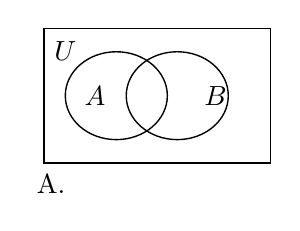
\begin{tikzpicture}[scale=0.9,line width=0.5pt]
\draw (0,0) rectangle (3.2,1.9);
\draw (1.02,0.95) ellipse (0.72 and 0.62);
\draw (1.88,0.95) ellipse (0.72 and 0.62);
\node at (0.72,0.95) {$A$};
\node at (2.42,0.95) {$B$};
\node at (0.3,1.58) {$U$};
\node[anchor=north] at (0.1,-0.03) {A.};
\end{tikzpicture}
&
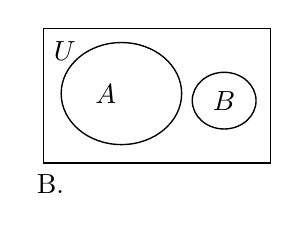
\begin{tikzpicture}[scale=0.9,line width=0.5pt]
\draw (0,0) rectangle (3.2,1.9);
\draw (1.1,0.98) ellipse (0.85 and 0.72);
\draw (2.55,0.88) ellipse (0.45 and 0.4);
\node at (0.88,0.98) {$A$};
\node at (2.55,0.88) {$B$};
\node at (0.3,1.58) {$U$};
\node[anchor=north] at (0.1,-0.03) {B.};
\end{tikzpicture}
\\[10pt]
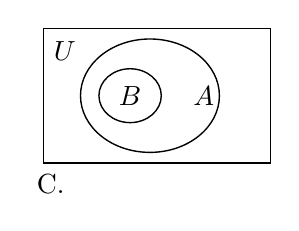
\begin{tikzpicture}[scale=0.9,line width=0.5pt]
\draw (0,0) rectangle (3.2,1.9);
\draw (1.5,0.95) ellipse (0.98 and 0.8);
\draw (1.22,0.95) ellipse (0.44 and 0.38);
\node at (1.22,0.95) {$B$};
\node at (2.26,0.95) {$A$};
\node at (0.3,1.58) {$U$};
\node[anchor=north] at (0.1,-0.03) {C.};
\end{tikzpicture}
&
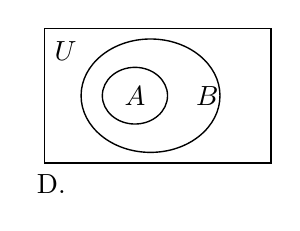
\begin{tikzpicture}[scale=0.9,line width=0.5pt]
\draw (0,0) rectangle (3.2,1.9);
\draw (1.5,0.95) ellipse (0.98 and 0.8);
\draw (1.28,0.95) ellipse (0.46 and 0.4);
\node at (1.28,0.95) {$A$};
\node at (2.3,0.95) {$B$};
\node at (0.3,1.58) {$U$};
\node[anchor=north] at (0.1,-0.03) {D.};
\end{tikzpicture}
\\
\end{tabular}
\end{center}

\ifanswer
\solbegin
\step{$\dfrac{2x-8}{x-5}\leqslant1\Rightarrow\dfrac{2x-8}{x-5}-1\leqslant0\Rightarrow\dfrac{x-3}{x-5}\leqslant0$，等价于 $\begin{cases}(x-3)(x-5)\leqslant0\\ x-5\neq0\end{cases}$，}
\step{解得 $3\leqslant x<5$，因为 $x\in\N$，所以 $A=\{3,4\}$，}
\step{解不等式 $x^2-7x+12\leqslant0$ 得 $B=\{x\mid3\leqslant x\leqslant4\}$，}
\step{集合 $A$ 中的元素 3，4 都属于集合 $B$，且 $B$ 中存在无数实数不属于 $A$，}
\step{所以 $A$ 是 $B$ 的真子集，$A$ 在 $B$ 内部．故选 $D$.}
\solend

\fi

\item 已知 $a$、$b$、$c\in\R$，则下列命题中真命题的个数是\mbox{（\quad）}

①若 $ac^2>bc^2$，则 $a>b$；②若 $\lvert a-2\rvert>\lvert b-2\rvert$，则 $(a-2)^2>(b-2)^2$；

③若 $a>b>c>0$，则 $\dfrac ab>\dfrac{a+c}{b+c}$；④若 $a>0$，$b>0$，$a+b>4$，$ab>4$，则 $a>2$，$b>2$.

\keepwithprev
A. $1$\qquad\qquad B. $2$\qquad\qquad C. $3$\qquad\qquad D. $4$

\ifanswer
\solbegin
\step{①若 $ac^2>bc^2$，则 $c^2>0$，则 $a>b$；所以①正确；}
\step{②若 $\lvert a-2\rvert>\lvert b-2\rvert$，则 $(a-2)^2>(b-2)^2$；满足不等式的基本性质，所以②正确；}
\step{③若 $a>b>c>0$，则 $\dfrac ab>\dfrac{a+c}{b+c}$；所以③正确；}
\step{④若 $a>0$，$b>0$，$a+b>4$，$ab>4$，则 $a>2$，$b>2$.}
\step{反例 $a=10$，$b=0.5$，满足条件，推不出结论，所以④不正确；}
\step{故选 $C$.}
\solend

\fi

\item 已知实数 $a<b$，关于 $x$ 的不等式 $x^2-(a+b)x+ab-1<0$ 的解集为 $(x_1,x_2)$，则实数
$a$、$b$、$x_1$、$x_2$ 从小到大的排列是\mbox{（\quad）}

\keepwithprev
A. $x_1<a<x_2<b$\qquad B. $x_1<a<b<x_2$\qquad C. $a<x_1<b<x_2$\qquad D. $a<x_1<x_2<b$

\ifanswer
\solbegin
\step{已知实数 $a<b$，关于 $x$ 的不等式 $x^2-(a+b)x+ab-1<0$ 的解集为 $(x_1,x_2)$，}
\step{因为 $x^2-(a+b)x+ab=(x-a)(x-b)$.}
\step{设函数 $g(x)=(x-a)(x-b)$，作函数 $g(x)$、$g(x)-1$ 的图象如下：}
\begin{center}
% 原图第 6 页解析插图直接裁取（原卷排于解析行右侧），已去粉色水印转灰度。
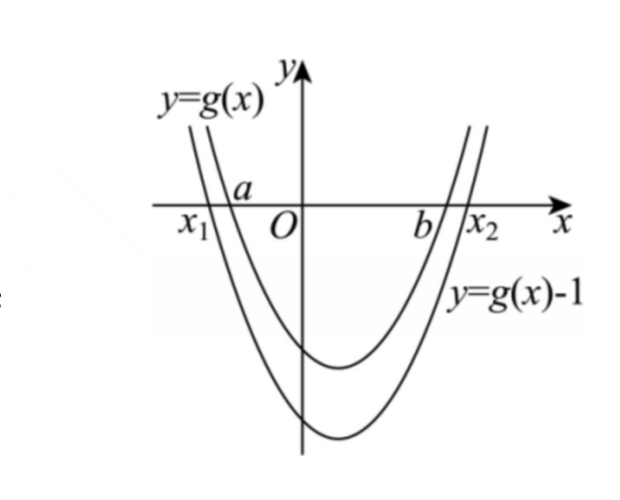
\includegraphics[width=0.20\textwidth]{figures/gao103_q16.png}
\end{center}
\step{由图像得 $x_1<a<b<x_2$．故选 $B$.}
\solend

\fi

\end{enumerate}

\bigsec{三、解答题}

\begin{enumerate}
\setcounter{enumi}{16}

\item 已知集合 $A=\{x\mid-3\leqslant x\leqslant1\}$，$B=\{x\mid a-2<x<a+2,a\in\R\}$.

（1）当 $a=1$ 时，求 $A\cap B$、$A\cup B$；

（2）若 $B\subseteq\overline A$，求 $a$ 的取值范围.

\ansspace*[8]

\ifanswer
\solbegin
\stepm{（1）}{当 $a=1$ 时，$B=\{x\mid-1<x<3\}$，又因为 $A=\{x\mid-3\leqslant x\leqslant1\}$，}
\step{所以 $A\cap B=\{x\mid-1<x\leqslant1\}$，$A\cup B=\{x\mid-3\leqslant x<3\}$；}
\stepm{（2）}{由 $A=\{x\mid-3\leqslant x\leqslant1\}$，得 $\overline A=\{x\mid x<-3\text{ 或 }x>1\}$，}
\step{若 $B\subseteq\overline A$，易得 $B=\{x\mid a-2<x<a+2,a\in\R\}\neq\varnothing$，}
\step{所以 $a+2\leqslant-3$ 或 $a-2\geqslant1$，解得 $a\leqslant-5$ 或 $a\geqslant3$，}
\step{综上所述，实数 $a$ 的取值范围是 $(-\infty,-5]\cup[3,+\infty)$.}
\solend

\fi

\item （1）解不等式 $\lvert 1-2x\rvert>x$；

（2）已知 $a$、$b$ 都是有理数，满足 $a+b\sqrt5=0$，请用反证法证明：$a=b=0$.

\ansspace*[10]

\ifanswer
\solbegin
\stepm{（1）}{①当 $x<0$ 时，左边非负，右边为负，不等式显然成立；}
\step{②当 $x\geqslant0$ 时，两边平方，$(1-2x)^2>x^2\Rightarrow3x^2-4x+1>0$}
\step{$\Rightarrow(3x-1)(x-1)>0$，解得 $x<\dfrac13$ 或 $x>1$，结合 $x\geqslant0$，}
\step{得 $0\leqslant x<\dfrac13$ 或 $x>1$；}
\step{综上，不等式解集为 $\left(-\infty,\dfrac13\right)\cup(1,+\infty)$.}
\stepm{（2）}{假设 $a,b$ 至少有一个不为零，}
\step{当 $a,b$ 中有一个为零一个不为零时，不妨设 $\begin{cases}a\neq0\\ b=0\end{cases}$，}
\step{则 $a+b\sqrt5=0\Rightarrow a=0$ 矛盾，舍；}
\step{当 $\begin{cases}a\neq0\\ b\neq0\end{cases}$ 时，$a+b\sqrt5=0\Rightarrow\sqrt5=-\dfrac ab\in\Q$，矛盾，舍，}
\step{综上假设不成立，所以 $a=b=0$.}
\solend

\fi

\item 某物流公司为了扩大业务量，计划建造一间高为 6 米，底面积为 24 平方米，且背面靠
墙的长方形形状的仓库。仓库的背面靠墙，无须建造费用，因此甲工程队给出的报价为：
仓库前面新建墙体每平方米 400 元，左右两面新建墙体每平方米 300 元，屋顶和地面以及
其他共计 28800 元.

（1）设仓库前面墙体的长为 $x$ 米 $(x>0)$，甲工程队的整体报价为 $y$ 元。若该物流公司计
划投入的改造资金不超过 60000 元，求前面墙体长 $x$ 的取值范围.

（2）在（1）的条件下，当仓库前面墙体的长度为多少时，甲工程队的整体
报价最低？

\begin{center}
% 原图第 7 页题干仓库示意图直接裁取（原卷排于题干右侧），已去粉色水印转灰度。
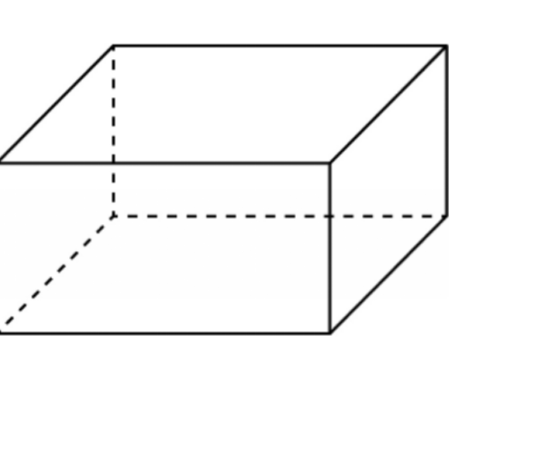
\includegraphics[width=0.17\textwidth]{figures/gao103_q19.png}
\end{center}

\ansspace*[12]

\ifanswer
\solbegin
\stepm{（1）}{甲队整体报价为 $y=400\times6x+2\times300\times6\times\dfrac{24}{x}+28800$}
\step{$=2400x+\dfrac{86400}{x}+28800$ 元，}
\step{要求 $y\leqslant60000$，即 $2400x+\dfrac{86400}{x}+28800\leqslant60000$，}
\step{化简得 $x+\dfrac{36}{x}\leqslant13$，}
\step{由于 $x>0$，则不等式化为 $x^2-13x+36\leqslant0$，}
\step{即 $(x-4)(x-9)\leqslant0$，解得 $4\leqslant x\leqslant9$，}
\step{所以前面墙体长 $x$ 的取值范围为 $[4,9]$；}
\stepm{（2）}{甲队整体报价为 $y=2400x+\dfrac{86400}{x}$}
\step{$\geqslant2\sqrt{2400x\times\dfrac{86400}{x}}+28800=57600$，}
\step{当且仅当 $2400x=\dfrac{86400}{x}$，即 $x^2=36$，}
\step{解得 $x=6$（满足 $4\leqslant x\leqslant9$）时取等号，}
\step{所以当仓库前面墙体的长度为 6 米时，甲工程队的整体报价最低，}
\step{为 57600 元.}
\solend

\fi

\item 已知函数 $f(x)=ax^2-10x+4b$.

（1）当 $a=1$，$b=4$ 时，解不等式 $f(x)\geqslant0$；

（2）若关于 $x$ 的不等式 $f(x)<0$ 的解集为 $(a,b)$，求实数 $a$、$b$ 的值；

（3）若 1 是 $f(x)$ 的零点，且 $a>0$，$b>0$，问当 $a$、$b$ 取何值时，$\dfrac1a+\dfrac1b$ 的值最小？最
小值是多少？

\ansspace*[12]

\ifanswer
\solbegin
\stepm{（1）}{将 $a=1$，$b=4$ 代入得 $f(x)=x^2-10x+16\geqslant0$，解得 $x\geqslant8$ 或 $x\leqslant2$，}
\step{所以不等式的解集为 $\{x\mid x\geqslant8\text{ 或 }x\leqslant2\}$；}
\stepm{（2）}{由题意得 $a$、$b$ 是 $ax^2-10x+4b=0$ 两根，且 $a<b$，$a>0$，}
\step{由韦达定理得 $\begin{cases}a+b=\dfrac{10}{a}\\ a\cdot b=\dfrac{4b}{a}\end{cases}$，解得 $\begin{cases}a=2\\ b=3\end{cases}$，即实数 $a$、$b$ 的值分别为 2，3；}
\stepm{（3）}{由 1 是 $f(x)$ 的零点，得 $f(1)=a-10+4b=0$，得 $a+4b=10$，}
\step{因为 $a>0$，$b>0$，}
\step{所以 $\dfrac1a+\dfrac1b=\dfrac1{10}\left(\dfrac1a+\dfrac1b\right)(a+4b)=\dfrac1{10}\left(1+4+\dfrac{4b}{a}+\dfrac ab\right)$}
\step{$\geqslant\dfrac1{10}\left(5+2\sqrt{\dfrac{4b}{a}\cdot\dfrac ab}\right)=\dfrac9{10}$，}
\step{当且仅当 $\dfrac{4b}{a}=\dfrac ab$，即 $a=\dfrac{10}3$,$b=\dfrac53$ 时取等号，}
\step{所以 $\dfrac1a+\dfrac1b$ 取最小值，且最小值为 $\dfrac9{10}$.}
\solend

\fi

\item 已知集合 $A$ 为非空集合，定义 $S=\{x\mid x=a+b,a,b\in A\}$，
$T=\{x\mid x=\lvert a-b\rvert,a,b\in A\}$.

（1）若集合 $A=\{1,3\}$，直接写出集合 $S$、$T$ (无需写计算过程)；

（2）若集合 $A=\{x_1,x_2,x_3,x_4\},x_1<x_2<x_3<x_4$，且 $T=A$，求证：$x_1+x_4=x_2+x_3$；

（3）若集合 $A=\{x\mid0\leqslant x\leqslant2026,x\in\N\}$,$S\cap T=\varnothing$．记 $\lvert A\rvert$ 为集合 $A$ 中元素的个数，求
$\lvert A\rvert$ 的最大值.

\ansspace*[16]

\ifanswer
\solbegin
\stepm{（1）}{$S=\{2,4,6\}$,$T=\{0,2\}$；}
\stepm{（2）}{集合 $T$ 中最小的元素为 0，因为 $T=A$，且 $x_1<x_2<x_3<x_4$，所以 $x_1=0$，}
\step{所以集合 $T$ 中元素为 $x_2-x_1=x_2$,$x_3-x_1=x_3$,$x_4-x_1=x_4$，}
\step{以及 $x_3-x_2$,$x_4-x_2$,$x_4-x_3$ 均属于 $A$，}
\step{因为 $x_1=0<x_3-x_2<x_4-x_2<x_4$，所以 $x_3$ 即 $x_4-x_2=x_3-x_1$，}
\step{即 $x_1+x_4=x_2+x_3$；}
\stepm{（3）}{设 $A=\{a_1,a_2,a_3,\cdots,a_k\}$ 满足题意，其中 $a_1<a_2<\cdots<a_k$，}
\step{则 $2a_1<a_1+a_2<\cdots<a_1+a_k<a_2+a_k<a_3+a_k<\cdots<a_{k-1}+a_k<2a_k$，}
\step{所以 $\lvert S\cup T\rvert\leqslant2k+1$，所以 $3k-1\leqslant2a_k+1\leqslant4053(k\in\N^*)$，}
\step{所以 $k\leqslant1351$，}
\step{实际上当 $A=\{676,677,\cdots,2026\}$ 时满足题意，}
\step{证明如下：设 $A=\{m,m+1,m+2,\cdots,2026\},m\in N$，}
\step{设 $S=\{2m,2m+1,2m+2,\cdots,4052\}$,$T=\{0,1,2,\cdots,2026-m\}$，}
\step{由题意得 $2026-m<2m$，即 $m>675\dfrac13$，}
\step{故 $m$ 的最小值是 676，于是当 $m=676$,$A$ 中的元素最多，}
\step{即 $A=\{676,677,\cdots,2026\}$ 时满足题意，}
\step{综上所述，集合 $A$ 中元素的个数的最大值是 1351.}
\solend

\fi

\end{enumerate}

\end{document}
"
%
% 原始材料：微信公众号“魔都数学加油站”文章，作者破晓，2026-11-01 21:56 发布；
% 连载“27学年高一103”，原文标题“27学年高一103——2026-2027年上海市市北中学高一上10月月考”；
% 原文链接：https://mp.weixin.qq.com/s/iBvF4eKw66F-kS6xLmDpBA。
% 正文为 10 张 PNG 页（第 1、3、5、6、7、10 页 2560×3620，其余 4762×6735），题目下印有【解析】，为讲评版。
% 题目、解析均据原图转录；卷面水印及公众号页脚未录入。
%
% 卷首标题：原卷印作“2026-2027 年市北中学高一上 10 月月考”（公众号标题中的“上海市”“高一上”
% 卷面标题行没有或已含，本稿照卷面），年份区间按全稿惯例排 en dash；原卷未印副标题，本稿按题目
% 内容标为“集合与常用逻辑用语、不等式”。
%
% 与原卷的排版差异：
%   ① 原文从第 3 题起，填空题编号为 3—12、选择题为 13—16、解答题为 17—21，本稿保留原题号；
%   ② 原卷每题下直接印【解析】，本稿按全稿惯例将解析置于答案版；选择题括号内未印答案，另由
%      解析末句“故选 X”给出；
%   ③ 原卷未印副标题，本稿按“知识模块”口径补出；
%   ④ 原卷填空横线按全稿惯例排为 \blankline[4.4em]；解答题按惯例加 \ansspace；选择题括号排
%      \mbox{（\quad）}；
%   ⑤ 原卷数集排斜体 $R$／$Q$（第 18 题解析 $Q$ 排粗体），按全稿惯例改 $\R$／$\Q$；
%   ⑥ 第 14 题四个文氏图选项按原图形状用 TikZ 重排；第 16、19 两题的插图裁自原图
%      （去粉色水印转灰度），第 19 题图属题干（三版都出），第 16 题图属解析（仅答案版显示）。
%
% 原卷存疑／笔误（均照录加注）：
%   第 9 题解析“故 $a+b=3b+b<0$”（$a=3b$ 代入应为 $4b$，原卷写作 $3b+b$，数值相同）；
%   第 21 题 (2) 解析“所以 $x_3$ 即 $x_4-x_2=x_3-x_1$”表述含糊（意为 $x_4-x_2$ 恰为 $T$ 中
%   介于 $x_2$ 与 $x_4$ 之间的元素 $x_3-x_1$）；
%   第 21 题 (3) 解析“所以 $|S\cup T|\leqslant2k+1$”（按上下文应为 $2a_k+1$，与后半句
%   $3k-1\leqslant2a_k+1$ 呼应），照录。
%
% 行数核对：逐题数 \step/\stepm 条数，合计 119 条（Q3：2；Q4：2；Q5：5；Q6：3；Q8：3；
% Q9：7；Q10：5；Q11：8；Q12：7；Q13：6；Q14：5；Q15：6；Q16：4；Q17：6；Q18：10；
% Q19：13；Q20：10；Q21：17），与原卷印刷行逐题相等。第 7 题只印【答案】，提 \ans{}，
% 不计入 \step 账。
%
\documentclass[a4paper,11pt]{article}
\usepackage{common}

\begin{document}

\examtitlest[3]{2026--2027 年市北中学高一上 10 月月考}{集合与常用逻辑用语、不等式}

\bigsec{一、填空题}

\begin{enumerate}
\setcounter{enumi}{2}

\item 已知实数 $x$ 满足 $\dfrac{7-x}{x+4}>0$，则 $x$ 的取值范围是\blankline[4.4em].

\ifanswer
\solbegin
\step{不等式 $\dfrac{7-x}{x+4}>0$ 可化为 $\dfrac{x-7}{x+4}<0$，等价于 $(x-7)(x+4)<0$，}
\step{解得 $-4<x<7$，所以 $x$ 的取值范围是 $\{x\mid-4<x<7\}$.}
\solend

\fi

\item 已知 $x_1$、$x_2$ 为方程 $2x^2+6x+3=0$ 的两个实数根，则 $\dfrac1{x_1}+\dfrac1{x_2}=$\blankline[4.4em].

\ifanswer
\solbegin
\step{由根与系数的关系得 $x_1+x_2=-\dfrac62=-3$，$x_1x_2=\dfrac32$，}
\step{则 $\dfrac1{x_1}+\dfrac1{x_2}=\dfrac{x_1+x_2}{x_1x_2}=-2$.}
\solend

\fi

\item 已知 $y=\lvert x-2\rvert+\lvert x-5\rvert$，$x\in\R$，则 $y$ 的最小值为\blankline[4.4em].

\ifanswer
\solbegin
\step{$y=\lvert x-2\rvert+\lvert x-5\rvert=\begin{cases}7-2x, & x<2\\ 3, & 2\leqslant x\leqslant5\\ 2x-7, & x>5\end{cases}$，}
\step{当 $x<2$ 时，$y>7-2\times2=3$；}
\step{当 $2\leqslant x\leqslant5$ 时，$y=3$；}
\step{当 $x>5$ 时，$y>2\times5-7=3$.}
\step{综上所述，$y$ 的最小值为 3.}
\solend

\fi

\item 对任意实数 $x$，等式 $ax^4+bx^3+cx^2+dx+e=x(x-2)(x^2+3)$ 恒成立，则
$b+c+d=$\blankline[4.4em].

\ifanswer
\solbegin
\step{因为 $ax^4+bx^3+cx^2+dx+e=x(x-2)(x^2+3)=(x^2-2x)(x^2+3)$}
\step{$=x^4-2x^3+3x^2-6x$，所以 $a=1$，$b=-2$，$c=3$，$d=-6$，$e=0$，}
\step{所以 $b+c+d=-2+3-6=-5$.}
\solend

\fi

\item 命题：“存在 $x\in(1,+\infty)$，使得 $ax^2+bx+c<0$”的否定形式是\blankline[4.4em].

\ifanswer
\ans{对于任意的 $x\in(1,+\infty)$，都有 $ax^2+bx+c\geqslant0$}
\fi

\item 已知集合 $A=\{x\mid mx^2-2x+1=0,x\in\R\}$ 有且仅有两个子集，则实数 $m=$\blankline[4.4em].

\ifanswer
\solbegin
\step{①当 $m=0$ 时，方程为 $-2x+1=0$，解得 $x=\dfrac12$，满足 $A=\left\{\dfrac12\right\}$ 仅有两个子集；}
\step{②当 $m\neq0$ 时，方程有两个相等实根，所以 $\Delta=4-4m=0$，解得 $m=1$；}
\step{所以实数 $m$ 的值为 0 或 1.}
\solend

\fi

\item 设 $a$、$b\in\R$，已知关于 $x$ 的不等式 $(a+b)x+(b-3a)<0$ 的解集为 $(2,+\infty)$，则不等式
$(a-2b)x+5b-a>0$ 的解集为\blankline[4.4em].

\ifanswer
\solbegin
\step{关于 $x$ 的不等式 $(a+b)x+(b-3a)<0$ 的解集为 $(2,+\infty)$，}
\step{得 $x=2$ 是 $(a+b)x+(b-3a)=0$ 的解，且 $a+b<0$，}
\step{所以 $2(a+b)+(b-3a)=0$，化简得 $a=3b$，故 $a+b=3b+b<0$，即 $b<0$，}
\step{将 $a=3b$ 代入 $(a-2b)x+5b-a>0$，}
\step{得不等式 $(a-2b)x+5b-a>0$ 即 $b(x+2)>0$，}
\step{两边都除以 $b$，得 $x+2<0$，解得 $x<-2$，}
\step{所以不等式 $(a-2b)x+5b-a>0$ 的解集为 $(-\infty,-2)$.}
\solend

\fi

\item 已知不等式 $\lvert x-a\rvert<1$ 成立的充分不必要条件是 $\dfrac12<x<\dfrac32$，则实数 $a$ 的取值范围
是\blankline[4.4em].

\ifanswer
\solbegin
\step{$\lvert x-a\rvert<1$，解得 $a-1<x<1+a$，}
\step{所以 $a-1<x<1+a$ 成立的充分不必要条件是 $\dfrac12<x<\dfrac32$，}
\step{故 $\left\{x\left|\dfrac12<x<\dfrac32\right.\right\}$ 是 $\{x\mid a-1<x<1+a\}$ 的真子集，}
\step{所以 $a-1\leqslant\dfrac12$ 且 $1+a\geqslant\dfrac32$（等号不同时成立），解得 $\dfrac12\leqslant a\leqslant\dfrac32$，}
\step{故实数 $a$ 的取值范围是 $\left[\dfrac12,\dfrac32\right]$.}
\solend

\fi

\item 定义 $A\nabla B=\left\{z\,\middle|\,z=xy+\dfrac xy,x\in A,y\in B\right\}$，设集合 $A=\{0,2\}$，$B=\{1,2\}$，$C=\{1\}$，
则集合 $(A\nabla B)\nabla C=$\blankline[4.4em].

\ifanswer
\solbegin
\step{当 $x=0$，$y=1$ 或 2 时，$z=xy+\dfrac xy=0$；}
\step{当 $x=2$，$y=1$ 时，$z=xy+\dfrac xy=4$；}
\step{当 $x=2$，$y=2$ 时，$z=xy+\dfrac xy=5$；}
\step{所以 $A\nabla B=\{0,4,5\}$；}
\step{当 $x=0$，$y=1$ 时，$z=xy+\dfrac xy=0$；}
\step{当 $x=4$，$y=1$ 时，$z=xy+\dfrac xy=8$；}
\step{当 $x=5$，$y=1$ 时，$z=xy+\dfrac xy=10$；}
\step{所以 $(A\nabla B)\nabla C=\{0,8,10\}$.}
\solend

\fi

\item 集合 $M=\{66,-11,23,10,911,-1,-18,100,0,\pi\}$ 有 10 个元素，设 $M$ 的所有非空子集为
$M_i\,(i=1,2,\cdots,1023)$，每一个 $M_i$ 中所有元素乘积为 $m_i\,(i=1,2,\cdots,1023)$，则
$m_1+m_2+m_3+\cdots+m_{1023}=$\blankline[4.4em].

\ifanswer
\solbegin
\step{因为 $M$ 的所有非空子集为 $M_i\,(i=1,2,\cdots,1023)$，这 1023 个子集分成以下几种情况：}
\step{①含 0 的子集有 512 个，这些子集均满足 $m_i=0$；}
\step{②不含 0，含 $-1$ 且还含有其它元素的子集有 255 个，}
\step{③不含 0，不含 $-1$ 但含有其它元素的子集有 255 个，}
\step{④只含 $-1$ 的子集一个 $\{-1\}$，满足 $m_i=-1$；}
\step{其中②③中的集合是一一对应的，且满足 $m_i$ 对应成相反数，}
\step{故 $m_1+m_2+m_3+\cdots+m_{1023}=512\times0+255\times0-1=-1$.}
\solend

\fi

\end{enumerate}

\bigsec{二、选择题}

\begin{enumerate}
\setcounter{enumi}{12}

\item 下列说法中，正确说法的个数是\mbox{（\quad）}

①联合国安理会常任理事国能组成一个集合；

②市北中学很喜欢足球的同学能组成一个集合；

③实数 $1,0,5,\dfrac12,\dfrac32,\dfrac64,\sqrt{\dfrac14}$ 组成的集合中有 6 个元素.

\keepwithprev
A. $0$\qquad\qquad B. $1$\qquad\qquad C. $2$\qquad\qquad D. $3$.

\ifanswer
\solbegin
\step{对于①，“联合国安理会常任理事国”满足集合的定义，故①正确；}
\step{对于②，“很喜欢”不满足集合的确定性，}
\step{市北中学很喜欢足球的同学不能组成一个集合，故②错误；}
\step{对于③，$\dfrac64=\dfrac32$，$\sqrt{\dfrac14}=\dfrac12$，由集合的元素互异性，集合中共有 5 个元素，}
\step{故③错误.}
\step{所以正确说法的个数是 1 个．故选 $B$.}
\solend

\fi

\item 已知全集 $U=\R$，集合 $A=\left\{x\,\middle|\,\dfrac{2x-8}{x-5}\leqslant1,x\in\N\right\}$，集合 $B=\{x\mid x^2-7x+12\leqslant0\}$，则
正确表示集合 $A$ 与集合 $B$ 关系的文氏图是\mbox{（\quad）}

\keepwithprev
\begin{center}
% 原卷四个文氏图选项按原图形状用 TikZ 重排。
\begin{tabular}{c@{\qquad\qquad}c}
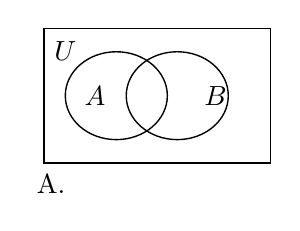
\begin{tikzpicture}[scale=0.9,line width=0.5pt]
\draw (0,0) rectangle (3.2,1.9);
\draw (1.02,0.95) ellipse (0.72 and 0.62);
\draw (1.88,0.95) ellipse (0.72 and 0.62);
\node at (0.72,0.95) {$A$};
\node at (2.42,0.95) {$B$};
\node at (0.3,1.58) {$U$};
\node[anchor=north] at (0.1,-0.03) {A.};
\end{tikzpicture}
&
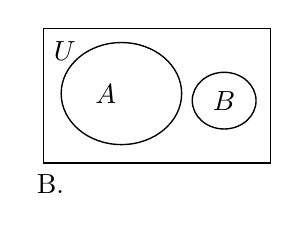
\begin{tikzpicture}[scale=0.9,line width=0.5pt]
\draw (0,0) rectangle (3.2,1.9);
\draw (1.1,0.98) ellipse (0.85 and 0.72);
\draw (2.55,0.88) ellipse (0.45 and 0.4);
\node at (0.88,0.98) {$A$};
\node at (2.55,0.88) {$B$};
\node at (0.3,1.58) {$U$};
\node[anchor=north] at (0.1,-0.03) {B.};
\end{tikzpicture}
\\[10pt]
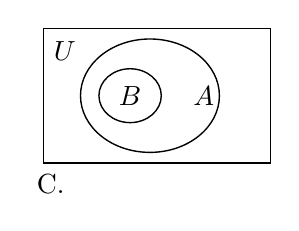
\begin{tikzpicture}[scale=0.9,line width=0.5pt]
\draw (0,0) rectangle (3.2,1.9);
\draw (1.5,0.95) ellipse (0.98 and 0.8);
\draw (1.22,0.95) ellipse (0.44 and 0.38);
\node at (1.22,0.95) {$B$};
\node at (2.26,0.95) {$A$};
\node at (0.3,1.58) {$U$};
\node[anchor=north] at (0.1,-0.03) {C.};
\end{tikzpicture}
&
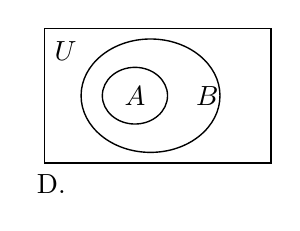
\begin{tikzpicture}[scale=0.9,line width=0.5pt]
\draw (0,0) rectangle (3.2,1.9);
\draw (1.5,0.95) ellipse (0.98 and 0.8);
\draw (1.28,0.95) ellipse (0.46 and 0.4);
\node at (1.28,0.95) {$A$};
\node at (2.3,0.95) {$B$};
\node at (0.3,1.58) {$U$};
\node[anchor=north] at (0.1,-0.03) {D.};
\end{tikzpicture}
\\
\end{tabular}
\end{center}

\ifanswer
\solbegin
\step{$\dfrac{2x-8}{x-5}\leqslant1\Rightarrow\dfrac{2x-8}{x-5}-1\leqslant0\Rightarrow\dfrac{x-3}{x-5}\leqslant0$，等价于 $\begin{cases}(x-3)(x-5)\leqslant0\\ x-5\neq0\end{cases}$，}
\step{解得 $3\leqslant x<5$，因为 $x\in\N$，所以 $A=\{3,4\}$，}
\step{解不等式 $x^2-7x+12\leqslant0$ 得 $B=\{x\mid3\leqslant x\leqslant4\}$，}
\step{集合 $A$ 中的元素 3，4 都属于集合 $B$，且 $B$ 中存在无数实数不属于 $A$，}
\step{所以 $A$ 是 $B$ 的真子集，$A$ 在 $B$ 内部．故选 $D$.}
\solend

\fi

\item 已知 $a$、$b$、$c\in\R$，则下列命题中真命题的个数是\mbox{（\quad）}

①若 $ac^2>bc^2$，则 $a>b$；②若 $\lvert a-2\rvert>\lvert b-2\rvert$，则 $(a-2)^2>(b-2)^2$；

③若 $a>b>c>0$，则 $\dfrac ab>\dfrac{a+c}{b+c}$；④若 $a>0$，$b>0$，$a+b>4$，$ab>4$，则 $a>2$，$b>2$.

\keepwithprev
A. $1$\qquad\qquad B. $2$\qquad\qquad C. $3$\qquad\qquad D. $4$

\ifanswer
\solbegin
\step{①若 $ac^2>bc^2$，则 $c^2>0$，则 $a>b$；所以①正确；}
\step{②若 $\lvert a-2\rvert>\lvert b-2\rvert$，则 $(a-2)^2>(b-2)^2$；满足不等式的基本性质，所以②正确；}
\step{③若 $a>b>c>0$，则 $\dfrac ab>\dfrac{a+c}{b+c}$；所以③正确；}
\step{④若 $a>0$，$b>0$，$a+b>4$，$ab>4$，则 $a>2$，$b>2$.}
\step{反例 $a=10$，$b=0.5$，满足条件，推不出结论，所以④不正确；}
\step{故选 $C$.}
\solend

\fi

\item 已知实数 $a<b$，关于 $x$ 的不等式 $x^2-(a+b)x+ab-1<0$ 的解集为 $(x_1,x_2)$，则实数
$a$、$b$、$x_1$、$x_2$ 从小到大的排列是\mbox{（\quad）}

\keepwithprev
A. $x_1<a<x_2<b$\qquad B. $x_1<a<b<x_2$\qquad C. $a<x_1<b<x_2$\qquad D. $a<x_1<x_2<b$

\ifanswer
\solbegin
\step{已知实数 $a<b$，关于 $x$ 的不等式 $x^2-(a+b)x+ab-1<0$ 的解集为 $(x_1,x_2)$，}
\step{因为 $x^2-(a+b)x+ab=(x-a)(x-b)$.}
\step{设函数 $g(x)=(x-a)(x-b)$，作函数 $g(x)$、$g(x)-1$ 的图象如下：}
\begin{center}
% 原图第 6 页解析插图直接裁取（原卷排于解析行右侧），已去粉色水印转灰度。
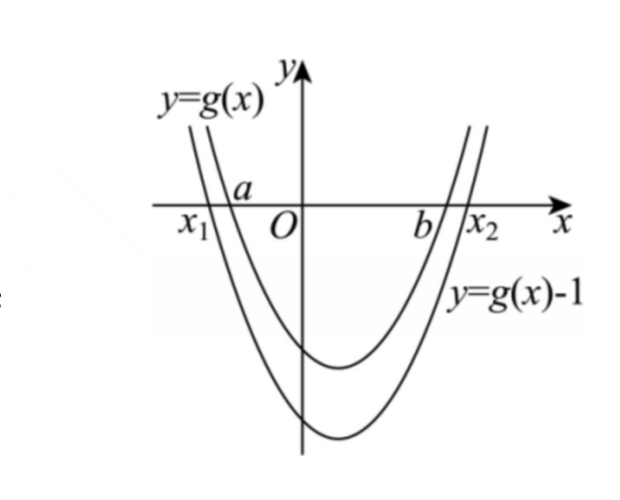
\includegraphics[width=0.20\textwidth]{figures/gao103_q16.png}
\end{center}
\step{由图像得 $x_1<a<b<x_2$．故选 $B$.}
\solend

\fi

\end{enumerate}

\bigsec{三、解答题}

\begin{enumerate}
\setcounter{enumi}{16}

\item 已知集合 $A=\{x\mid-3\leqslant x\leqslant1\}$，$B=\{x\mid a-2<x<a+2,a\in\R\}$.

（1）当 $a=1$ 时，求 $A\cap B$、$A\cup B$；

（2）若 $B\subseteq\overline A$，求 $a$ 的取值范围.

\ansspace*[8]

\ifanswer
\solbegin
\stepm{（1）}{当 $a=1$ 时，$B=\{x\mid-1<x<3\}$，又因为 $A=\{x\mid-3\leqslant x\leqslant1\}$，}
\step{所以 $A\cap B=\{x\mid-1<x\leqslant1\}$，$A\cup B=\{x\mid-3\leqslant x<3\}$；}
\stepm{（2）}{由 $A=\{x\mid-3\leqslant x\leqslant1\}$，得 $\overline A=\{x\mid x<-3\text{ 或 }x>1\}$，}
\step{若 $B\subseteq\overline A$，易得 $B=\{x\mid a-2<x<a+2,a\in\R\}\neq\varnothing$，}
\step{所以 $a+2\leqslant-3$ 或 $a-2\geqslant1$，解得 $a\leqslant-5$ 或 $a\geqslant3$，}
\step{综上所述，实数 $a$ 的取值范围是 $(-\infty,-5]\cup[3,+\infty)$.}
\solend

\fi

\item （1）解不等式 $\lvert 1-2x\rvert>x$；

（2）已知 $a$、$b$ 都是有理数，满足 $a+b\sqrt5=0$，请用反证法证明：$a=b=0$.

\ansspace*[10]

\ifanswer
\solbegin
\stepm{（1）}{①当 $x<0$ 时，左边非负，右边为负，不等式显然成立；}
\step{②当 $x\geqslant0$ 时，两边平方，$(1-2x)^2>x^2\Rightarrow3x^2-4x+1>0$}
\step{$\Rightarrow(3x-1)(x-1)>0$，解得 $x<\dfrac13$ 或 $x>1$，结合 $x\geqslant0$，}
\step{得 $0\leqslant x<\dfrac13$ 或 $x>1$；}
\step{综上，不等式解集为 $\left(-\infty,\dfrac13\right)\cup(1,+\infty)$.}
\stepm{（2）}{假设 $a,b$ 至少有一个不为零，}
\step{当 $a,b$ 中有一个为零一个不为零时，不妨设 $\begin{cases}a\neq0\\ b=0\end{cases}$，}
\step{则 $a+b\sqrt5=0\Rightarrow a=0$ 矛盾，舍；}
\step{当 $\begin{cases}a\neq0\\ b\neq0\end{cases}$ 时，$a+b\sqrt5=0\Rightarrow\sqrt5=-\dfrac ab\in\Q$，矛盾，舍，}
\step{综上假设不成立，所以 $a=b=0$.}
\solend

\fi

\item 某物流公司为了扩大业务量，计划建造一间高为 6 米，底面积为 24 平方米，且背面靠
墙的长方形形状的仓库。仓库的背面靠墙，无须建造费用，因此甲工程队给出的报价为：
仓库前面新建墙体每平方米 400 元，左右两面新建墙体每平方米 300 元，屋顶和地面以及
其他共计 28800 元.

（1）设仓库前面墙体的长为 $x$ 米 $(x>0)$，甲工程队的整体报价为 $y$ 元。若该物流公司计
划投入的改造资金不超过 60000 元，求前面墙体长 $x$ 的取值范围.

（2）在（1）的条件下，当仓库前面墙体的长度为多少时，甲工程队的整体
报价最低？

\begin{center}
% 原图第 7 页题干仓库示意图直接裁取（原卷排于题干右侧），已去粉色水印转灰度。
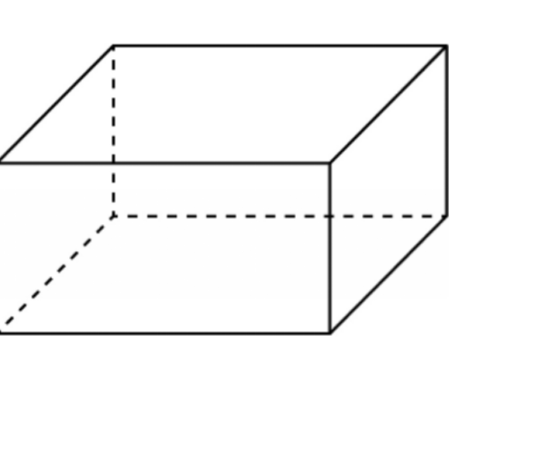
\includegraphics[width=0.17\textwidth]{figures/gao103_q19.png}
\end{center}

\ansspace*[12]

\ifanswer
\solbegin
\stepm{（1）}{甲队整体报价为 $y=400\times6x+2\times300\times6\times\dfrac{24}{x}+28800$}
\step{$=2400x+\dfrac{86400}{x}+28800$ 元，}
\step{要求 $y\leqslant60000$，即 $2400x+\dfrac{86400}{x}+28800\leqslant60000$，}
\step{化简得 $x+\dfrac{36}{x}\leqslant13$，}
\step{由于 $x>0$，则不等式化为 $x^2-13x+36\leqslant0$，}
\step{即 $(x-4)(x-9)\leqslant0$，解得 $4\leqslant x\leqslant9$，}
\step{所以前面墙体长 $x$ 的取值范围为 $[4,9]$；}
\stepm{（2）}{甲队整体报价为 $y=2400x+\dfrac{86400}{x}$}
\step{$\geqslant2\sqrt{2400x\times\dfrac{86400}{x}}+28800=57600$，}
\step{当且仅当 $2400x=\dfrac{86400}{x}$，即 $x^2=36$，}
\step{解得 $x=6$（满足 $4\leqslant x\leqslant9$）时取等号，}
\step{所以当仓库前面墙体的长度为 6 米时，甲工程队的整体报价最低，}
\step{为 57600 元.}
\solend

\fi

\item 已知函数 $f(x)=ax^2-10x+4b$.

（1）当 $a=1$，$b=4$ 时，解不等式 $f(x)\geqslant0$；

（2）若关于 $x$ 的不等式 $f(x)<0$ 的解集为 $(a,b)$，求实数 $a$、$b$ 的值；

（3）若 1 是 $f(x)$ 的零点，且 $a>0$，$b>0$，问当 $a$、$b$ 取何值时，$\dfrac1a+\dfrac1b$ 的值最小？最
小值是多少？

\ansspace*[12]

\ifanswer
\solbegin
\stepm{（1）}{将 $a=1$，$b=4$ 代入得 $f(x)=x^2-10x+16\geqslant0$，解得 $x\geqslant8$ 或 $x\leqslant2$，}
\step{所以不等式的解集为 $\{x\mid x\geqslant8\text{ 或 }x\leqslant2\}$；}
\stepm{（2）}{由题意得 $a$、$b$ 是 $ax^2-10x+4b=0$ 两根，且 $a<b$，$a>0$，}
\step{由韦达定理得 $\begin{cases}a+b=\dfrac{10}{a}\\ a\cdot b=\dfrac{4b}{a}\end{cases}$，解得 $\begin{cases}a=2\\ b=3\end{cases}$，即实数 $a$、$b$ 的值分别为 2，3；}
\stepm{（3）}{由 1 是 $f(x)$ 的零点，得 $f(1)=a-10+4b=0$，得 $a+4b=10$，}
\step{因为 $a>0$，$b>0$，}
\step{所以 $\dfrac1a+\dfrac1b=\dfrac1{10}\left(\dfrac1a+\dfrac1b\right)(a+4b)=\dfrac1{10}\left(1+4+\dfrac{4b}{a}+\dfrac ab\right)$}
\step{$\geqslant\dfrac1{10}\left(5+2\sqrt{\dfrac{4b}{a}\cdot\dfrac ab}\right)=\dfrac9{10}$，}
\step{当且仅当 $\dfrac{4b}{a}=\dfrac ab$，即 $a=\dfrac{10}3$,$b=\dfrac53$ 时取等号，}
\step{所以 $\dfrac1a+\dfrac1b$ 取最小值，且最小值为 $\dfrac9{10}$.}
\solend

\fi

\item 已知集合 $A$ 为非空集合，定义 $S=\{x\mid x=a+b,a,b\in A\}$，
$T=\{x\mid x=\lvert a-b\rvert,a,b\in A\}$.

（1）若集合 $A=\{1,3\}$，直接写出集合 $S$、$T$ (无需写计算过程)；

（2）若集合 $A=\{x_1,x_2,x_3,x_4\},x_1<x_2<x_3<x_4$，且 $T=A$，求证：$x_1+x_4=x_2+x_3$；

（3）若集合 $A=\{x\mid0\leqslant x\leqslant2026,x\in\N\}$,$S\cap T=\varnothing$．记 $\lvert A\rvert$ 为集合 $A$ 中元素的个数，求
$\lvert A\rvert$ 的最大值.

\ansspace*[16]

\ifanswer
\solbegin
\stepm{（1）}{$S=\{2,4,6\}$,$T=\{0,2\}$；}
\stepm{（2）}{集合 $T$ 中最小的元素为 0，因为 $T=A$，且 $x_1<x_2<x_3<x_4$，所以 $x_1=0$，}
\step{所以集合 $T$ 中元素为 $x_2-x_1=x_2$,$x_3-x_1=x_3$,$x_4-x_1=x_4$，}
\step{以及 $x_3-x_2$,$x_4-x_2$,$x_4-x_3$ 均属于 $A$，}
\step{因为 $x_1=0<x_3-x_2<x_4-x_2<x_4$，所以 $x_3$ 即 $x_4-x_2=x_3-x_1$，}
\step{即 $x_1+x_4=x_2+x_3$；}
\stepm{（3）}{设 $A=\{a_1,a_2,a_3,\cdots,a_k\}$ 满足题意，其中 $a_1<a_2<\cdots<a_k$，}
\step{则 $2a_1<a_1+a_2<\cdots<a_1+a_k<a_2+a_k<a_3+a_k<\cdots<a_{k-1}+a_k<2a_k$，}
\step{所以 $\lvert S\cup T\rvert\leqslant2k+1$，所以 $3k-1\leqslant2a_k+1\leqslant4053(k\in\N^*)$，}
\step{所以 $k\leqslant1351$，}
\step{实际上当 $A=\{676,677,\cdots,2026\}$ 时满足题意，}
\step{证明如下：设 $A=\{m,m+1,m+2,\cdots,2026\},m\in N$，}
\step{设 $S=\{2m,2m+1,2m+2,\cdots,4052\}$,$T=\{0,1,2,\cdots,2026-m\}$，}
\step{由题意得 $2026-m<2m$，即 $m>675\dfrac13$，}
\step{故 $m$ 的最小值是 676，于是当 $m=676$,$A$ 中的元素最多，}
\step{即 $A=\{676,677,\cdots,2026\}$ 时满足题意，}
\step{综上所述，集合 $A$ 中元素的个数的最大值是 1351.}
\solend

\fi

\end{enumerate}

\end{document}
"
% 紧凑版：xelatex "\def\iscompact{1}% 高一103_市北中学_10月月考.tex
%   —— 高一上数学“2026-2027 年市北中学高一上 10 月月考”（试卷版/答案版）
% 试卷版：xelatex 高一103_市北中学_10月月考.tex
% 答案版：xelatex "\def\isanswer{1}% 高一103_市北中学_10月月考.tex
%   —— 高一上数学“2026-2027 年市北中学高一上 10 月月考”（试卷版/答案版）
% 试卷版：xelatex 高一103_市北中学_10月月考.tex
% 答案版：xelatex "\def\isanswer{1}\input{高一103_市北中学_10月月考.tex}"
% 紧凑版：xelatex "\def\iscompact{1}\input{高一103_市北中学_10月月考.tex}"
%
% 原始材料：微信公众号“魔都数学加油站”文章，作者破晓，2026-11-01 21:56 发布；
% 连载“27学年高一103”，原文标题“27学年高一103——2026-2027年上海市市北中学高一上10月月考”；
% 原文链接：https://mp.weixin.qq.com/s/iBvF4eKw66F-kS6xLmDpBA。
% 正文为 10 张 PNG 页（第 1、3、5、6、7、10 页 2560×3620，其余 4762×6735），题目下印有【解析】，为讲评版。
% 题目、解析均据原图转录；卷面水印及公众号页脚未录入。
%
% 卷首标题：原卷印作“2026-2027 年市北中学高一上 10 月月考”（公众号标题中的“上海市”“高一上”
% 卷面标题行没有或已含，本稿照卷面），年份区间按全稿惯例排 en dash；原卷未印副标题，本稿按题目
% 内容标为“集合与常用逻辑用语、不等式”。
%
% 与原卷的排版差异：
%   ① 原文从第 3 题起，填空题编号为 3—12、选择题为 13—16、解答题为 17—21，本稿保留原题号；
%   ② 原卷每题下直接印【解析】，本稿按全稿惯例将解析置于答案版；选择题括号内未印答案，另由
%      解析末句“故选 X”给出；
%   ③ 原卷未印副标题，本稿按“知识模块”口径补出；
%   ④ 原卷填空横线按全稿惯例排为 \blankline[4.4em]；解答题按惯例加 \ansspace；选择题括号排
%      \mbox{（\quad）}；
%   ⑤ 原卷数集排斜体 $R$／$Q$（第 18 题解析 $Q$ 排粗体），按全稿惯例改 $\R$／$\Q$；
%   ⑥ 第 14 题四个文氏图选项按原图形状用 TikZ 重排；第 16、19 两题的插图裁自原图
%      （去粉色水印转灰度），第 19 题图属题干（三版都出），第 16 题图属解析（仅答案版显示）。
%
% 原卷存疑／笔误（均照录加注）：
%   第 9 题解析“故 $a+b=3b+b<0$”（$a=3b$ 代入应为 $4b$，原卷写作 $3b+b$，数值相同）；
%   第 21 题 (2) 解析“所以 $x_3$ 即 $x_4-x_2=x_3-x_1$”表述含糊（意为 $x_4-x_2$ 恰为 $T$ 中
%   介于 $x_2$ 与 $x_4$ 之间的元素 $x_3-x_1$）；
%   第 21 题 (3) 解析“所以 $|S\cup T|\leqslant2k+1$”（按上下文应为 $2a_k+1$，与后半句
%   $3k-1\leqslant2a_k+1$ 呼应），照录。
%
% 行数核对：逐题数 \step/\stepm 条数，合计 119 条（Q3：2；Q4：2；Q5：5；Q6：3；Q8：3；
% Q9：7；Q10：5；Q11：8；Q12：7；Q13：6；Q14：5；Q15：6；Q16：4；Q17：6；Q18：10；
% Q19：13；Q20：10；Q21：17），与原卷印刷行逐题相等。第 7 题只印【答案】，提 \ans{}，
% 不计入 \step 账。
%
\documentclass[a4paper,11pt]{article}
\usepackage{common}

\begin{document}

\examtitlest[3]{2026--2027 年市北中学高一上 10 月月考}{集合与常用逻辑用语、不等式}

\bigsec{一、填空题}

\begin{enumerate}
\setcounter{enumi}{2}

\item 已知实数 $x$ 满足 $\dfrac{7-x}{x+4}>0$，则 $x$ 的取值范围是\blankline[4.4em].

\ifanswer
\solbegin
\step{不等式 $\dfrac{7-x}{x+4}>0$ 可化为 $\dfrac{x-7}{x+4}<0$，等价于 $(x-7)(x+4)<0$，}
\step{解得 $-4<x<7$，所以 $x$ 的取值范围是 $\{x\mid-4<x<7\}$.}
\solend

\fi

\item 已知 $x_1$、$x_2$ 为方程 $2x^2+6x+3=0$ 的两个实数根，则 $\dfrac1{x_1}+\dfrac1{x_2}=$\blankline[4.4em].

\ifanswer
\solbegin
\step{由根与系数的关系得 $x_1+x_2=-\dfrac62=-3$，$x_1x_2=\dfrac32$，}
\step{则 $\dfrac1{x_1}+\dfrac1{x_2}=\dfrac{x_1+x_2}{x_1x_2}=-2$.}
\solend

\fi

\item 已知 $y=\lvert x-2\rvert+\lvert x-5\rvert$，$x\in\R$，则 $y$ 的最小值为\blankline[4.4em].

\ifanswer
\solbegin
\step{$y=\lvert x-2\rvert+\lvert x-5\rvert=\begin{cases}7-2x, & x<2\\ 3, & 2\leqslant x\leqslant5\\ 2x-7, & x>5\end{cases}$，}
\step{当 $x<2$ 时，$y>7-2\times2=3$；}
\step{当 $2\leqslant x\leqslant5$ 时，$y=3$；}
\step{当 $x>5$ 时，$y>2\times5-7=3$.}
\step{综上所述，$y$ 的最小值为 3.}
\solend

\fi

\item 对任意实数 $x$，等式 $ax^4+bx^3+cx^2+dx+e=x(x-2)(x^2+3)$ 恒成立，则
$b+c+d=$\blankline[4.4em].

\ifanswer
\solbegin
\step{因为 $ax^4+bx^3+cx^2+dx+e=x(x-2)(x^2+3)=(x^2-2x)(x^2+3)$}
\step{$=x^4-2x^3+3x^2-6x$，所以 $a=1$，$b=-2$，$c=3$，$d=-6$，$e=0$，}
\step{所以 $b+c+d=-2+3-6=-5$.}
\solend

\fi

\item 命题：“存在 $x\in(1,+\infty)$，使得 $ax^2+bx+c<0$”的否定形式是\blankline[4.4em].

\ifanswer
\ans{对于任意的 $x\in(1,+\infty)$，都有 $ax^2+bx+c\geqslant0$}
\fi

\item 已知集合 $A=\{x\mid mx^2-2x+1=0,x\in\R\}$ 有且仅有两个子集，则实数 $m=$\blankline[4.4em].

\ifanswer
\solbegin
\step{①当 $m=0$ 时，方程为 $-2x+1=0$，解得 $x=\dfrac12$，满足 $A=\left\{\dfrac12\right\}$ 仅有两个子集；}
\step{②当 $m\neq0$ 时，方程有两个相等实根，所以 $\Delta=4-4m=0$，解得 $m=1$；}
\step{所以实数 $m$ 的值为 0 或 1.}
\solend

\fi

\item 设 $a$、$b\in\R$，已知关于 $x$ 的不等式 $(a+b)x+(b-3a)<0$ 的解集为 $(2,+\infty)$，则不等式
$(a-2b)x+5b-a>0$ 的解集为\blankline[4.4em].

\ifanswer
\solbegin
\step{关于 $x$ 的不等式 $(a+b)x+(b-3a)<0$ 的解集为 $(2,+\infty)$，}
\step{得 $x=2$ 是 $(a+b)x+(b-3a)=0$ 的解，且 $a+b<0$，}
\step{所以 $2(a+b)+(b-3a)=0$，化简得 $a=3b$，故 $a+b=3b+b<0$，即 $b<0$，}
\step{将 $a=3b$ 代入 $(a-2b)x+5b-a>0$，}
\step{得不等式 $(a-2b)x+5b-a>0$ 即 $b(x+2)>0$，}
\step{两边都除以 $b$，得 $x+2<0$，解得 $x<-2$，}
\step{所以不等式 $(a-2b)x+5b-a>0$ 的解集为 $(-\infty,-2)$.}
\solend

\fi

\item 已知不等式 $\lvert x-a\rvert<1$ 成立的充分不必要条件是 $\dfrac12<x<\dfrac32$，则实数 $a$ 的取值范围
是\blankline[4.4em].

\ifanswer
\solbegin
\step{$\lvert x-a\rvert<1$，解得 $a-1<x<1+a$，}
\step{所以 $a-1<x<1+a$ 成立的充分不必要条件是 $\dfrac12<x<\dfrac32$，}
\step{故 $\left\{x\left|\dfrac12<x<\dfrac32\right.\right\}$ 是 $\{x\mid a-1<x<1+a\}$ 的真子集，}
\step{所以 $a-1\leqslant\dfrac12$ 且 $1+a\geqslant\dfrac32$（等号不同时成立），解得 $\dfrac12\leqslant a\leqslant\dfrac32$，}
\step{故实数 $a$ 的取值范围是 $\left[\dfrac12,\dfrac32\right]$.}
\solend

\fi

\item 定义 $A\nabla B=\left\{z\,\middle|\,z=xy+\dfrac xy,x\in A,y\in B\right\}$，设集合 $A=\{0,2\}$，$B=\{1,2\}$，$C=\{1\}$，
则集合 $(A\nabla B)\nabla C=$\blankline[4.4em].

\ifanswer
\solbegin
\step{当 $x=0$，$y=1$ 或 2 时，$z=xy+\dfrac xy=0$；}
\step{当 $x=2$，$y=1$ 时，$z=xy+\dfrac xy=4$；}
\step{当 $x=2$，$y=2$ 时，$z=xy+\dfrac xy=5$；}
\step{所以 $A\nabla B=\{0,4,5\}$；}
\step{当 $x=0$，$y=1$ 时，$z=xy+\dfrac xy=0$；}
\step{当 $x=4$，$y=1$ 时，$z=xy+\dfrac xy=8$；}
\step{当 $x=5$，$y=1$ 时，$z=xy+\dfrac xy=10$；}
\step{所以 $(A\nabla B)\nabla C=\{0,8,10\}$.}
\solend

\fi

\item 集合 $M=\{66,-11,23,10,911,-1,-18,100,0,\pi\}$ 有 10 个元素，设 $M$ 的所有非空子集为
$M_i\,(i=1,2,\cdots,1023)$，每一个 $M_i$ 中所有元素乘积为 $m_i\,(i=1,2,\cdots,1023)$，则
$m_1+m_2+m_3+\cdots+m_{1023}=$\blankline[4.4em].

\ifanswer
\solbegin
\step{因为 $M$ 的所有非空子集为 $M_i\,(i=1,2,\cdots,1023)$，这 1023 个子集分成以下几种情况：}
\step{①含 0 的子集有 512 个，这些子集均满足 $m_i=0$；}
\step{②不含 0，含 $-1$ 且还含有其它元素的子集有 255 个，}
\step{③不含 0，不含 $-1$ 但含有其它元素的子集有 255 个，}
\step{④只含 $-1$ 的子集一个 $\{-1\}$，满足 $m_i=-1$；}
\step{其中②③中的集合是一一对应的，且满足 $m_i$ 对应成相反数，}
\step{故 $m_1+m_2+m_3+\cdots+m_{1023}=512\times0+255\times0-1=-1$.}
\solend

\fi

\end{enumerate}

\bigsec{二、选择题}

\begin{enumerate}
\setcounter{enumi}{12}

\item 下列说法中，正确说法的个数是\mbox{（\quad）}

①联合国安理会常任理事国能组成一个集合；

②市北中学很喜欢足球的同学能组成一个集合；

③实数 $1,0,5,\dfrac12,\dfrac32,\dfrac64,\sqrt{\dfrac14}$ 组成的集合中有 6 个元素.

\keepwithprev
A. $0$\qquad\qquad B. $1$\qquad\qquad C. $2$\qquad\qquad D. $3$.

\ifanswer
\solbegin
\step{对于①，“联合国安理会常任理事国”满足集合的定义，故①正确；}
\step{对于②，“很喜欢”不满足集合的确定性，}
\step{市北中学很喜欢足球的同学不能组成一个集合，故②错误；}
\step{对于③，$\dfrac64=\dfrac32$，$\sqrt{\dfrac14}=\dfrac12$，由集合的元素互异性，集合中共有 5 个元素，}
\step{故③错误.}
\step{所以正确说法的个数是 1 个．故选 $B$.}
\solend

\fi

\item 已知全集 $U=\R$，集合 $A=\left\{x\,\middle|\,\dfrac{2x-8}{x-5}\leqslant1,x\in\N\right\}$，集合 $B=\{x\mid x^2-7x+12\leqslant0\}$，则
正确表示集合 $A$ 与集合 $B$ 关系的文氏图是\mbox{（\quad）}

\keepwithprev
\begin{center}
% 原卷四个文氏图选项按原图形状用 TikZ 重排。
\begin{tabular}{c@{\qquad\qquad}c}
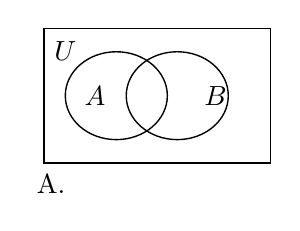
\begin{tikzpicture}[scale=0.9,line width=0.5pt]
\draw (0,0) rectangle (3.2,1.9);
\draw (1.02,0.95) ellipse (0.72 and 0.62);
\draw (1.88,0.95) ellipse (0.72 and 0.62);
\node at (0.72,0.95) {$A$};
\node at (2.42,0.95) {$B$};
\node at (0.3,1.58) {$U$};
\node[anchor=north] at (0.1,-0.03) {A.};
\end{tikzpicture}
&
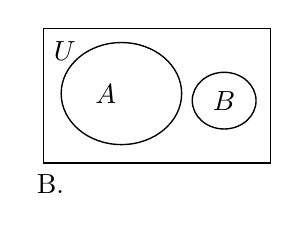
\begin{tikzpicture}[scale=0.9,line width=0.5pt]
\draw (0,0) rectangle (3.2,1.9);
\draw (1.1,0.98) ellipse (0.85 and 0.72);
\draw (2.55,0.88) ellipse (0.45 and 0.4);
\node at (0.88,0.98) {$A$};
\node at (2.55,0.88) {$B$};
\node at (0.3,1.58) {$U$};
\node[anchor=north] at (0.1,-0.03) {B.};
\end{tikzpicture}
\\[10pt]
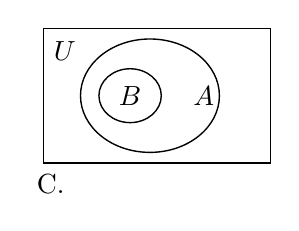
\begin{tikzpicture}[scale=0.9,line width=0.5pt]
\draw (0,0) rectangle (3.2,1.9);
\draw (1.5,0.95) ellipse (0.98 and 0.8);
\draw (1.22,0.95) ellipse (0.44 and 0.38);
\node at (1.22,0.95) {$B$};
\node at (2.26,0.95) {$A$};
\node at (0.3,1.58) {$U$};
\node[anchor=north] at (0.1,-0.03) {C.};
\end{tikzpicture}
&
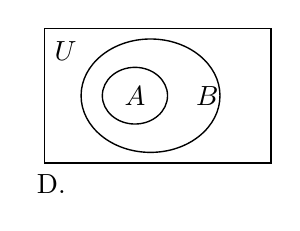
\begin{tikzpicture}[scale=0.9,line width=0.5pt]
\draw (0,0) rectangle (3.2,1.9);
\draw (1.5,0.95) ellipse (0.98 and 0.8);
\draw (1.28,0.95) ellipse (0.46 and 0.4);
\node at (1.28,0.95) {$A$};
\node at (2.3,0.95) {$B$};
\node at (0.3,1.58) {$U$};
\node[anchor=north] at (0.1,-0.03) {D.};
\end{tikzpicture}
\\
\end{tabular}
\end{center}

\ifanswer
\solbegin
\step{$\dfrac{2x-8}{x-5}\leqslant1\Rightarrow\dfrac{2x-8}{x-5}-1\leqslant0\Rightarrow\dfrac{x-3}{x-5}\leqslant0$，等价于 $\begin{cases}(x-3)(x-5)\leqslant0\\ x-5\neq0\end{cases}$，}
\step{解得 $3\leqslant x<5$，因为 $x\in\N$，所以 $A=\{3,4\}$，}
\step{解不等式 $x^2-7x+12\leqslant0$ 得 $B=\{x\mid3\leqslant x\leqslant4\}$，}
\step{集合 $A$ 中的元素 3，4 都属于集合 $B$，且 $B$ 中存在无数实数不属于 $A$，}
\step{所以 $A$ 是 $B$ 的真子集，$A$ 在 $B$ 内部．故选 $D$.}
\solend

\fi

\item 已知 $a$、$b$、$c\in\R$，则下列命题中真命题的个数是\mbox{（\quad）}

①若 $ac^2>bc^2$，则 $a>b$；②若 $\lvert a-2\rvert>\lvert b-2\rvert$，则 $(a-2)^2>(b-2)^2$；

③若 $a>b>c>0$，则 $\dfrac ab>\dfrac{a+c}{b+c}$；④若 $a>0$，$b>0$，$a+b>4$，$ab>4$，则 $a>2$，$b>2$.

\keepwithprev
A. $1$\qquad\qquad B. $2$\qquad\qquad C. $3$\qquad\qquad D. $4$

\ifanswer
\solbegin
\step{①若 $ac^2>bc^2$，则 $c^2>0$，则 $a>b$；所以①正确；}
\step{②若 $\lvert a-2\rvert>\lvert b-2\rvert$，则 $(a-2)^2>(b-2)^2$；满足不等式的基本性质，所以②正确；}
\step{③若 $a>b>c>0$，则 $\dfrac ab>\dfrac{a+c}{b+c}$；所以③正确；}
\step{④若 $a>0$，$b>0$，$a+b>4$，$ab>4$，则 $a>2$，$b>2$.}
\step{反例 $a=10$，$b=0.5$，满足条件，推不出结论，所以④不正确；}
\step{故选 $C$.}
\solend

\fi

\item 已知实数 $a<b$，关于 $x$ 的不等式 $x^2-(a+b)x+ab-1<0$ 的解集为 $(x_1,x_2)$，则实数
$a$、$b$、$x_1$、$x_2$ 从小到大的排列是\mbox{（\quad）}

\keepwithprev
A. $x_1<a<x_2<b$\qquad B. $x_1<a<b<x_2$\qquad C. $a<x_1<b<x_2$\qquad D. $a<x_1<x_2<b$

\ifanswer
\solbegin
\step{已知实数 $a<b$，关于 $x$ 的不等式 $x^2-(a+b)x+ab-1<0$ 的解集为 $(x_1,x_2)$，}
\step{因为 $x^2-(a+b)x+ab=(x-a)(x-b)$.}
\step{设函数 $g(x)=(x-a)(x-b)$，作函数 $g(x)$、$g(x)-1$ 的图象如下：}
\begin{center}
% 原图第 6 页解析插图直接裁取（原卷排于解析行右侧），已去粉色水印转灰度。
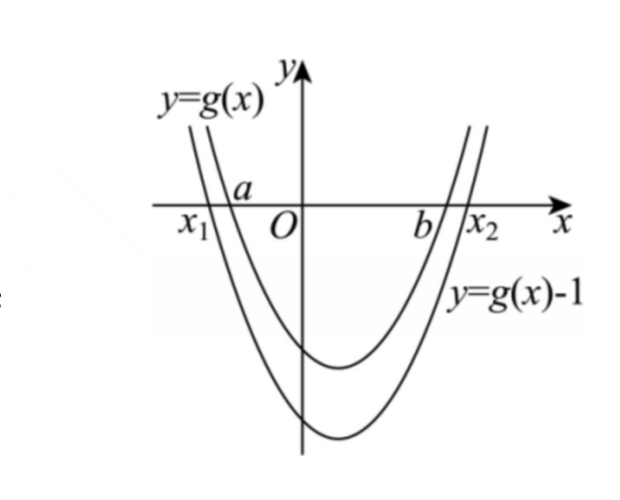
\includegraphics[width=0.20\textwidth]{figures/gao103_q16.png}
\end{center}
\step{由图像得 $x_1<a<b<x_2$．故选 $B$.}
\solend

\fi

\end{enumerate}

\bigsec{三、解答题}

\begin{enumerate}
\setcounter{enumi}{16}

\item 已知集合 $A=\{x\mid-3\leqslant x\leqslant1\}$，$B=\{x\mid a-2<x<a+2,a\in\R\}$.

（1）当 $a=1$ 时，求 $A\cap B$、$A\cup B$；

（2）若 $B\subseteq\overline A$，求 $a$ 的取值范围.

\ansspace*[8]

\ifanswer
\solbegin
\stepm{（1）}{当 $a=1$ 时，$B=\{x\mid-1<x<3\}$，又因为 $A=\{x\mid-3\leqslant x\leqslant1\}$，}
\step{所以 $A\cap B=\{x\mid-1<x\leqslant1\}$，$A\cup B=\{x\mid-3\leqslant x<3\}$；}
\stepm{（2）}{由 $A=\{x\mid-3\leqslant x\leqslant1\}$，得 $\overline A=\{x\mid x<-3\text{ 或 }x>1\}$，}
\step{若 $B\subseteq\overline A$，易得 $B=\{x\mid a-2<x<a+2,a\in\R\}\neq\varnothing$，}
\step{所以 $a+2\leqslant-3$ 或 $a-2\geqslant1$，解得 $a\leqslant-5$ 或 $a\geqslant3$，}
\step{综上所述，实数 $a$ 的取值范围是 $(-\infty,-5]\cup[3,+\infty)$.}
\solend

\fi

\item （1）解不等式 $\lvert 1-2x\rvert>x$；

（2）已知 $a$、$b$ 都是有理数，满足 $a+b\sqrt5=0$，请用反证法证明：$a=b=0$.

\ansspace*[10]

\ifanswer
\solbegin
\stepm{（1）}{①当 $x<0$ 时，左边非负，右边为负，不等式显然成立；}
\step{②当 $x\geqslant0$ 时，两边平方，$(1-2x)^2>x^2\Rightarrow3x^2-4x+1>0$}
\step{$\Rightarrow(3x-1)(x-1)>0$，解得 $x<\dfrac13$ 或 $x>1$，结合 $x\geqslant0$，}
\step{得 $0\leqslant x<\dfrac13$ 或 $x>1$；}
\step{综上，不等式解集为 $\left(-\infty,\dfrac13\right)\cup(1,+\infty)$.}
\stepm{（2）}{假设 $a,b$ 至少有一个不为零，}
\step{当 $a,b$ 中有一个为零一个不为零时，不妨设 $\begin{cases}a\neq0\\ b=0\end{cases}$，}
\step{则 $a+b\sqrt5=0\Rightarrow a=0$ 矛盾，舍；}
\step{当 $\begin{cases}a\neq0\\ b\neq0\end{cases}$ 时，$a+b\sqrt5=0\Rightarrow\sqrt5=-\dfrac ab\in\Q$，矛盾，舍，}
\step{综上假设不成立，所以 $a=b=0$.}
\solend

\fi

\item 某物流公司为了扩大业务量，计划建造一间高为 6 米，底面积为 24 平方米，且背面靠
墙的长方形形状的仓库。仓库的背面靠墙，无须建造费用，因此甲工程队给出的报价为：
仓库前面新建墙体每平方米 400 元，左右两面新建墙体每平方米 300 元，屋顶和地面以及
其他共计 28800 元.

（1）设仓库前面墙体的长为 $x$ 米 $(x>0)$，甲工程队的整体报价为 $y$ 元。若该物流公司计
划投入的改造资金不超过 60000 元，求前面墙体长 $x$ 的取值范围.

（2）在（1）的条件下，当仓库前面墙体的长度为多少时，甲工程队的整体
报价最低？

\begin{center}
% 原图第 7 页题干仓库示意图直接裁取（原卷排于题干右侧），已去粉色水印转灰度。
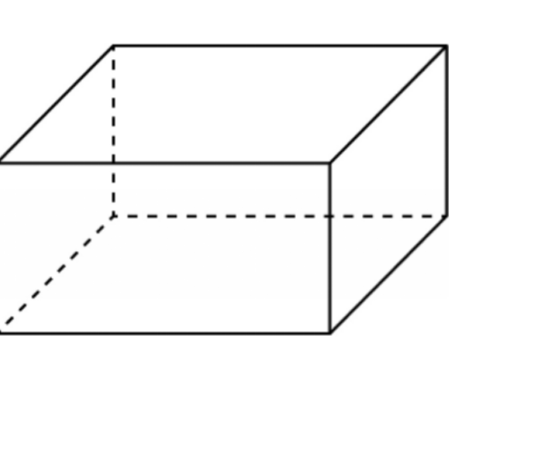
\includegraphics[width=0.17\textwidth]{figures/gao103_q19.png}
\end{center}

\ansspace*[12]

\ifanswer
\solbegin
\stepm{（1）}{甲队整体报价为 $y=400\times6x+2\times300\times6\times\dfrac{24}{x}+28800$}
\step{$=2400x+\dfrac{86400}{x}+28800$ 元，}
\step{要求 $y\leqslant60000$，即 $2400x+\dfrac{86400}{x}+28800\leqslant60000$，}
\step{化简得 $x+\dfrac{36}{x}\leqslant13$，}
\step{由于 $x>0$，则不等式化为 $x^2-13x+36\leqslant0$，}
\step{即 $(x-4)(x-9)\leqslant0$，解得 $4\leqslant x\leqslant9$，}
\step{所以前面墙体长 $x$ 的取值范围为 $[4,9]$；}
\stepm{（2）}{甲队整体报价为 $y=2400x+\dfrac{86400}{x}$}
\step{$\geqslant2\sqrt{2400x\times\dfrac{86400}{x}}+28800=57600$，}
\step{当且仅当 $2400x=\dfrac{86400}{x}$，即 $x^2=36$，}
\step{解得 $x=6$（满足 $4\leqslant x\leqslant9$）时取等号，}
\step{所以当仓库前面墙体的长度为 6 米时，甲工程队的整体报价最低，}
\step{为 57600 元.}
\solend

\fi

\item 已知函数 $f(x)=ax^2-10x+4b$.

（1）当 $a=1$，$b=4$ 时，解不等式 $f(x)\geqslant0$；

（2）若关于 $x$ 的不等式 $f(x)<0$ 的解集为 $(a,b)$，求实数 $a$、$b$ 的值；

（3）若 1 是 $f(x)$ 的零点，且 $a>0$，$b>0$，问当 $a$、$b$ 取何值时，$\dfrac1a+\dfrac1b$ 的值最小？最
小值是多少？

\ansspace*[12]

\ifanswer
\solbegin
\stepm{（1）}{将 $a=1$，$b=4$ 代入得 $f(x)=x^2-10x+16\geqslant0$，解得 $x\geqslant8$ 或 $x\leqslant2$，}
\step{所以不等式的解集为 $\{x\mid x\geqslant8\text{ 或 }x\leqslant2\}$；}
\stepm{（2）}{由题意得 $a$、$b$ 是 $ax^2-10x+4b=0$ 两根，且 $a<b$，$a>0$，}
\step{由韦达定理得 $\begin{cases}a+b=\dfrac{10}{a}\\ a\cdot b=\dfrac{4b}{a}\end{cases}$，解得 $\begin{cases}a=2\\ b=3\end{cases}$，即实数 $a$、$b$ 的值分别为 2，3；}
\stepm{（3）}{由 1 是 $f(x)$ 的零点，得 $f(1)=a-10+4b=0$，得 $a+4b=10$，}
\step{因为 $a>0$，$b>0$，}
\step{所以 $\dfrac1a+\dfrac1b=\dfrac1{10}\left(\dfrac1a+\dfrac1b\right)(a+4b)=\dfrac1{10}\left(1+4+\dfrac{4b}{a}+\dfrac ab\right)$}
\step{$\geqslant\dfrac1{10}\left(5+2\sqrt{\dfrac{4b}{a}\cdot\dfrac ab}\right)=\dfrac9{10}$，}
\step{当且仅当 $\dfrac{4b}{a}=\dfrac ab$，即 $a=\dfrac{10}3$,$b=\dfrac53$ 时取等号，}
\step{所以 $\dfrac1a+\dfrac1b$ 取最小值，且最小值为 $\dfrac9{10}$.}
\solend

\fi

\item 已知集合 $A$ 为非空集合，定义 $S=\{x\mid x=a+b,a,b\in A\}$，
$T=\{x\mid x=\lvert a-b\rvert,a,b\in A\}$.

（1）若集合 $A=\{1,3\}$，直接写出集合 $S$、$T$ (无需写计算过程)；

（2）若集合 $A=\{x_1,x_2,x_3,x_4\},x_1<x_2<x_3<x_4$，且 $T=A$，求证：$x_1+x_4=x_2+x_3$；

（3）若集合 $A=\{x\mid0\leqslant x\leqslant2026,x\in\N\}$,$S\cap T=\varnothing$．记 $\lvert A\rvert$ 为集合 $A$ 中元素的个数，求
$\lvert A\rvert$ 的最大值.

\ansspace*[16]

\ifanswer
\solbegin
\stepm{（1）}{$S=\{2,4,6\}$,$T=\{0,2\}$；}
\stepm{（2）}{集合 $T$ 中最小的元素为 0，因为 $T=A$，且 $x_1<x_2<x_3<x_4$，所以 $x_1=0$，}
\step{所以集合 $T$ 中元素为 $x_2-x_1=x_2$,$x_3-x_1=x_3$,$x_4-x_1=x_4$，}
\step{以及 $x_3-x_2$,$x_4-x_2$,$x_4-x_3$ 均属于 $A$，}
\step{因为 $x_1=0<x_3-x_2<x_4-x_2<x_4$，所以 $x_3$ 即 $x_4-x_2=x_3-x_1$，}
\step{即 $x_1+x_4=x_2+x_3$；}
\stepm{（3）}{设 $A=\{a_1,a_2,a_3,\cdots,a_k\}$ 满足题意，其中 $a_1<a_2<\cdots<a_k$，}
\step{则 $2a_1<a_1+a_2<\cdots<a_1+a_k<a_2+a_k<a_3+a_k<\cdots<a_{k-1}+a_k<2a_k$，}
\step{所以 $\lvert S\cup T\rvert\leqslant2k+1$，所以 $3k-1\leqslant2a_k+1\leqslant4053(k\in\N^*)$，}
\step{所以 $k\leqslant1351$，}
\step{实际上当 $A=\{676,677,\cdots,2026\}$ 时满足题意，}
\step{证明如下：设 $A=\{m,m+1,m+2,\cdots,2026\},m\in N$，}
\step{设 $S=\{2m,2m+1,2m+2,\cdots,4052\}$,$T=\{0,1,2,\cdots,2026-m\}$，}
\step{由题意得 $2026-m<2m$，即 $m>675\dfrac13$，}
\step{故 $m$ 的最小值是 676，于是当 $m=676$,$A$ 中的元素最多，}
\step{即 $A=\{676,677,\cdots,2026\}$ 时满足题意，}
\step{综上所述，集合 $A$ 中元素的个数的最大值是 1351.}
\solend

\fi

\end{enumerate}

\end{document}
"
% 紧凑版：xelatex "\def\iscompact{1}% 高一103_市北中学_10月月考.tex
%   —— 高一上数学“2026-2027 年市北中学高一上 10 月月考”（试卷版/答案版）
% 试卷版：xelatex 高一103_市北中学_10月月考.tex
% 答案版：xelatex "\def\isanswer{1}\input{高一103_市北中学_10月月考.tex}"
% 紧凑版：xelatex "\def\iscompact{1}\input{高一103_市北中学_10月月考.tex}"
%
% 原始材料：微信公众号“魔都数学加油站”文章，作者破晓，2026-11-01 21:56 发布；
% 连载“27学年高一103”，原文标题“27学年高一103——2026-2027年上海市市北中学高一上10月月考”；
% 原文链接：https://mp.weixin.qq.com/s/iBvF4eKw66F-kS6xLmDpBA。
% 正文为 10 张 PNG 页（第 1、3、5、6、7、10 页 2560×3620，其余 4762×6735），题目下印有【解析】，为讲评版。
% 题目、解析均据原图转录；卷面水印及公众号页脚未录入。
%
% 卷首标题：原卷印作“2026-2027 年市北中学高一上 10 月月考”（公众号标题中的“上海市”“高一上”
% 卷面标题行没有或已含，本稿照卷面），年份区间按全稿惯例排 en dash；原卷未印副标题，本稿按题目
% 内容标为“集合与常用逻辑用语、不等式”。
%
% 与原卷的排版差异：
%   ① 原文从第 3 题起，填空题编号为 3—12、选择题为 13—16、解答题为 17—21，本稿保留原题号；
%   ② 原卷每题下直接印【解析】，本稿按全稿惯例将解析置于答案版；选择题括号内未印答案，另由
%      解析末句“故选 X”给出；
%   ③ 原卷未印副标题，本稿按“知识模块”口径补出；
%   ④ 原卷填空横线按全稿惯例排为 \blankline[4.4em]；解答题按惯例加 \ansspace；选择题括号排
%      \mbox{（\quad）}；
%   ⑤ 原卷数集排斜体 $R$／$Q$（第 18 题解析 $Q$ 排粗体），按全稿惯例改 $\R$／$\Q$；
%   ⑥ 第 14 题四个文氏图选项按原图形状用 TikZ 重排；第 16、19 两题的插图裁自原图
%      （去粉色水印转灰度），第 19 题图属题干（三版都出），第 16 题图属解析（仅答案版显示）。
%
% 原卷存疑／笔误（均照录加注）：
%   第 9 题解析“故 $a+b=3b+b<0$”（$a=3b$ 代入应为 $4b$，原卷写作 $3b+b$，数值相同）；
%   第 21 题 (2) 解析“所以 $x_3$ 即 $x_4-x_2=x_3-x_1$”表述含糊（意为 $x_4-x_2$ 恰为 $T$ 中
%   介于 $x_2$ 与 $x_4$ 之间的元素 $x_3-x_1$）；
%   第 21 题 (3) 解析“所以 $|S\cup T|\leqslant2k+1$”（按上下文应为 $2a_k+1$，与后半句
%   $3k-1\leqslant2a_k+1$ 呼应），照录。
%
% 行数核对：逐题数 \step/\stepm 条数，合计 119 条（Q3：2；Q4：2；Q5：5；Q6：3；Q8：3；
% Q9：7；Q10：5；Q11：8；Q12：7；Q13：6；Q14：5；Q15：6；Q16：4；Q17：6；Q18：10；
% Q19：13；Q20：10；Q21：17），与原卷印刷行逐题相等。第 7 题只印【答案】，提 \ans{}，
% 不计入 \step 账。
%
\documentclass[a4paper,11pt]{article}
\usepackage{common}

\begin{document}

\examtitlest[3]{2026--2027 年市北中学高一上 10 月月考}{集合与常用逻辑用语、不等式}

\bigsec{一、填空题}

\begin{enumerate}
\setcounter{enumi}{2}

\item 已知实数 $x$ 满足 $\dfrac{7-x}{x+4}>0$，则 $x$ 的取值范围是\blankline[4.4em].

\ifanswer
\solbegin
\step{不等式 $\dfrac{7-x}{x+4}>0$ 可化为 $\dfrac{x-7}{x+4}<0$，等价于 $(x-7)(x+4)<0$，}
\step{解得 $-4<x<7$，所以 $x$ 的取值范围是 $\{x\mid-4<x<7\}$.}
\solend

\fi

\item 已知 $x_1$、$x_2$ 为方程 $2x^2+6x+3=0$ 的两个实数根，则 $\dfrac1{x_1}+\dfrac1{x_2}=$\blankline[4.4em].

\ifanswer
\solbegin
\step{由根与系数的关系得 $x_1+x_2=-\dfrac62=-3$，$x_1x_2=\dfrac32$，}
\step{则 $\dfrac1{x_1}+\dfrac1{x_2}=\dfrac{x_1+x_2}{x_1x_2}=-2$.}
\solend

\fi

\item 已知 $y=\lvert x-2\rvert+\lvert x-5\rvert$，$x\in\R$，则 $y$ 的最小值为\blankline[4.4em].

\ifanswer
\solbegin
\step{$y=\lvert x-2\rvert+\lvert x-5\rvert=\begin{cases}7-2x, & x<2\\ 3, & 2\leqslant x\leqslant5\\ 2x-7, & x>5\end{cases}$，}
\step{当 $x<2$ 时，$y>7-2\times2=3$；}
\step{当 $2\leqslant x\leqslant5$ 时，$y=3$；}
\step{当 $x>5$ 时，$y>2\times5-7=3$.}
\step{综上所述，$y$ 的最小值为 3.}
\solend

\fi

\item 对任意实数 $x$，等式 $ax^4+bx^3+cx^2+dx+e=x(x-2)(x^2+3)$ 恒成立，则
$b+c+d=$\blankline[4.4em].

\ifanswer
\solbegin
\step{因为 $ax^4+bx^3+cx^2+dx+e=x(x-2)(x^2+3)=(x^2-2x)(x^2+3)$}
\step{$=x^4-2x^3+3x^2-6x$，所以 $a=1$，$b=-2$，$c=3$，$d=-6$，$e=0$，}
\step{所以 $b+c+d=-2+3-6=-5$.}
\solend

\fi

\item 命题：“存在 $x\in(1,+\infty)$，使得 $ax^2+bx+c<0$”的否定形式是\blankline[4.4em].

\ifanswer
\ans{对于任意的 $x\in(1,+\infty)$，都有 $ax^2+bx+c\geqslant0$}
\fi

\item 已知集合 $A=\{x\mid mx^2-2x+1=0,x\in\R\}$ 有且仅有两个子集，则实数 $m=$\blankline[4.4em].

\ifanswer
\solbegin
\step{①当 $m=0$ 时，方程为 $-2x+1=0$，解得 $x=\dfrac12$，满足 $A=\left\{\dfrac12\right\}$ 仅有两个子集；}
\step{②当 $m\neq0$ 时，方程有两个相等实根，所以 $\Delta=4-4m=0$，解得 $m=1$；}
\step{所以实数 $m$ 的值为 0 或 1.}
\solend

\fi

\item 设 $a$、$b\in\R$，已知关于 $x$ 的不等式 $(a+b)x+(b-3a)<0$ 的解集为 $(2,+\infty)$，则不等式
$(a-2b)x+5b-a>0$ 的解集为\blankline[4.4em].

\ifanswer
\solbegin
\step{关于 $x$ 的不等式 $(a+b)x+(b-3a)<0$ 的解集为 $(2,+\infty)$，}
\step{得 $x=2$ 是 $(a+b)x+(b-3a)=0$ 的解，且 $a+b<0$，}
\step{所以 $2(a+b)+(b-3a)=0$，化简得 $a=3b$，故 $a+b=3b+b<0$，即 $b<0$，}
\step{将 $a=3b$ 代入 $(a-2b)x+5b-a>0$，}
\step{得不等式 $(a-2b)x+5b-a>0$ 即 $b(x+2)>0$，}
\step{两边都除以 $b$，得 $x+2<0$，解得 $x<-2$，}
\step{所以不等式 $(a-2b)x+5b-a>0$ 的解集为 $(-\infty,-2)$.}
\solend

\fi

\item 已知不等式 $\lvert x-a\rvert<1$ 成立的充分不必要条件是 $\dfrac12<x<\dfrac32$，则实数 $a$ 的取值范围
是\blankline[4.4em].

\ifanswer
\solbegin
\step{$\lvert x-a\rvert<1$，解得 $a-1<x<1+a$，}
\step{所以 $a-1<x<1+a$ 成立的充分不必要条件是 $\dfrac12<x<\dfrac32$，}
\step{故 $\left\{x\left|\dfrac12<x<\dfrac32\right.\right\}$ 是 $\{x\mid a-1<x<1+a\}$ 的真子集，}
\step{所以 $a-1\leqslant\dfrac12$ 且 $1+a\geqslant\dfrac32$（等号不同时成立），解得 $\dfrac12\leqslant a\leqslant\dfrac32$，}
\step{故实数 $a$ 的取值范围是 $\left[\dfrac12,\dfrac32\right]$.}
\solend

\fi

\item 定义 $A\nabla B=\left\{z\,\middle|\,z=xy+\dfrac xy,x\in A,y\in B\right\}$，设集合 $A=\{0,2\}$，$B=\{1,2\}$，$C=\{1\}$，
则集合 $(A\nabla B)\nabla C=$\blankline[4.4em].

\ifanswer
\solbegin
\step{当 $x=0$，$y=1$ 或 2 时，$z=xy+\dfrac xy=0$；}
\step{当 $x=2$，$y=1$ 时，$z=xy+\dfrac xy=4$；}
\step{当 $x=2$，$y=2$ 时，$z=xy+\dfrac xy=5$；}
\step{所以 $A\nabla B=\{0,4,5\}$；}
\step{当 $x=0$，$y=1$ 时，$z=xy+\dfrac xy=0$；}
\step{当 $x=4$，$y=1$ 时，$z=xy+\dfrac xy=8$；}
\step{当 $x=5$，$y=1$ 时，$z=xy+\dfrac xy=10$；}
\step{所以 $(A\nabla B)\nabla C=\{0,8,10\}$.}
\solend

\fi

\item 集合 $M=\{66,-11,23,10,911,-1,-18,100,0,\pi\}$ 有 10 个元素，设 $M$ 的所有非空子集为
$M_i\,(i=1,2,\cdots,1023)$，每一个 $M_i$ 中所有元素乘积为 $m_i\,(i=1,2,\cdots,1023)$，则
$m_1+m_2+m_3+\cdots+m_{1023}=$\blankline[4.4em].

\ifanswer
\solbegin
\step{因为 $M$ 的所有非空子集为 $M_i\,(i=1,2,\cdots,1023)$，这 1023 个子集分成以下几种情况：}
\step{①含 0 的子集有 512 个，这些子集均满足 $m_i=0$；}
\step{②不含 0，含 $-1$ 且还含有其它元素的子集有 255 个，}
\step{③不含 0，不含 $-1$ 但含有其它元素的子集有 255 个，}
\step{④只含 $-1$ 的子集一个 $\{-1\}$，满足 $m_i=-1$；}
\step{其中②③中的集合是一一对应的，且满足 $m_i$ 对应成相反数，}
\step{故 $m_1+m_2+m_3+\cdots+m_{1023}=512\times0+255\times0-1=-1$.}
\solend

\fi

\end{enumerate}

\bigsec{二、选择题}

\begin{enumerate}
\setcounter{enumi}{12}

\item 下列说法中，正确说法的个数是\mbox{（\quad）}

①联合国安理会常任理事国能组成一个集合；

②市北中学很喜欢足球的同学能组成一个集合；

③实数 $1,0,5,\dfrac12,\dfrac32,\dfrac64,\sqrt{\dfrac14}$ 组成的集合中有 6 个元素.

\keepwithprev
A. $0$\qquad\qquad B. $1$\qquad\qquad C. $2$\qquad\qquad D. $3$.

\ifanswer
\solbegin
\step{对于①，“联合国安理会常任理事国”满足集合的定义，故①正确；}
\step{对于②，“很喜欢”不满足集合的确定性，}
\step{市北中学很喜欢足球的同学不能组成一个集合，故②错误；}
\step{对于③，$\dfrac64=\dfrac32$，$\sqrt{\dfrac14}=\dfrac12$，由集合的元素互异性，集合中共有 5 个元素，}
\step{故③错误.}
\step{所以正确说法的个数是 1 个．故选 $B$.}
\solend

\fi

\item 已知全集 $U=\R$，集合 $A=\left\{x\,\middle|\,\dfrac{2x-8}{x-5}\leqslant1,x\in\N\right\}$，集合 $B=\{x\mid x^2-7x+12\leqslant0\}$，则
正确表示集合 $A$ 与集合 $B$ 关系的文氏图是\mbox{（\quad）}

\keepwithprev
\begin{center}
% 原卷四个文氏图选项按原图形状用 TikZ 重排。
\begin{tabular}{c@{\qquad\qquad}c}
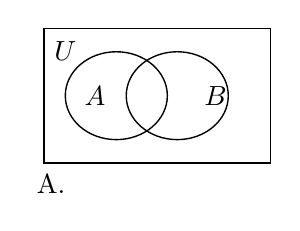
\begin{tikzpicture}[scale=0.9,line width=0.5pt]
\draw (0,0) rectangle (3.2,1.9);
\draw (1.02,0.95) ellipse (0.72 and 0.62);
\draw (1.88,0.95) ellipse (0.72 and 0.62);
\node at (0.72,0.95) {$A$};
\node at (2.42,0.95) {$B$};
\node at (0.3,1.58) {$U$};
\node[anchor=north] at (0.1,-0.03) {A.};
\end{tikzpicture}
&
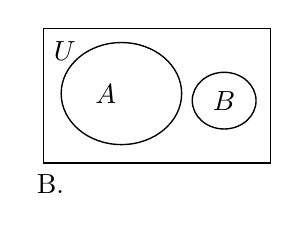
\begin{tikzpicture}[scale=0.9,line width=0.5pt]
\draw (0,0) rectangle (3.2,1.9);
\draw (1.1,0.98) ellipse (0.85 and 0.72);
\draw (2.55,0.88) ellipse (0.45 and 0.4);
\node at (0.88,0.98) {$A$};
\node at (2.55,0.88) {$B$};
\node at (0.3,1.58) {$U$};
\node[anchor=north] at (0.1,-0.03) {B.};
\end{tikzpicture}
\\[10pt]
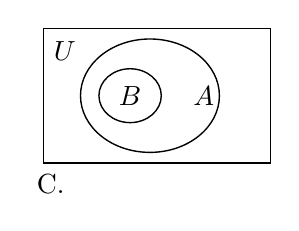
\begin{tikzpicture}[scale=0.9,line width=0.5pt]
\draw (0,0) rectangle (3.2,1.9);
\draw (1.5,0.95) ellipse (0.98 and 0.8);
\draw (1.22,0.95) ellipse (0.44 and 0.38);
\node at (1.22,0.95) {$B$};
\node at (2.26,0.95) {$A$};
\node at (0.3,1.58) {$U$};
\node[anchor=north] at (0.1,-0.03) {C.};
\end{tikzpicture}
&
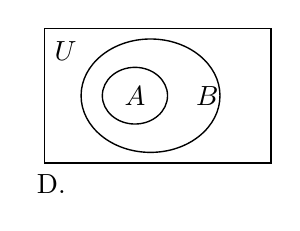
\begin{tikzpicture}[scale=0.9,line width=0.5pt]
\draw (0,0) rectangle (3.2,1.9);
\draw (1.5,0.95) ellipse (0.98 and 0.8);
\draw (1.28,0.95) ellipse (0.46 and 0.4);
\node at (1.28,0.95) {$A$};
\node at (2.3,0.95) {$B$};
\node at (0.3,1.58) {$U$};
\node[anchor=north] at (0.1,-0.03) {D.};
\end{tikzpicture}
\\
\end{tabular}
\end{center}

\ifanswer
\solbegin
\step{$\dfrac{2x-8}{x-5}\leqslant1\Rightarrow\dfrac{2x-8}{x-5}-1\leqslant0\Rightarrow\dfrac{x-3}{x-5}\leqslant0$，等价于 $\begin{cases}(x-3)(x-5)\leqslant0\\ x-5\neq0\end{cases}$，}
\step{解得 $3\leqslant x<5$，因为 $x\in\N$，所以 $A=\{3,4\}$，}
\step{解不等式 $x^2-7x+12\leqslant0$ 得 $B=\{x\mid3\leqslant x\leqslant4\}$，}
\step{集合 $A$ 中的元素 3，4 都属于集合 $B$，且 $B$ 中存在无数实数不属于 $A$，}
\step{所以 $A$ 是 $B$ 的真子集，$A$ 在 $B$ 内部．故选 $D$.}
\solend

\fi

\item 已知 $a$、$b$、$c\in\R$，则下列命题中真命题的个数是\mbox{（\quad）}

①若 $ac^2>bc^2$，则 $a>b$；②若 $\lvert a-2\rvert>\lvert b-2\rvert$，则 $(a-2)^2>(b-2)^2$；

③若 $a>b>c>0$，则 $\dfrac ab>\dfrac{a+c}{b+c}$；④若 $a>0$，$b>0$，$a+b>4$，$ab>4$，则 $a>2$，$b>2$.

\keepwithprev
A. $1$\qquad\qquad B. $2$\qquad\qquad C. $3$\qquad\qquad D. $4$

\ifanswer
\solbegin
\step{①若 $ac^2>bc^2$，则 $c^2>0$，则 $a>b$；所以①正确；}
\step{②若 $\lvert a-2\rvert>\lvert b-2\rvert$，则 $(a-2)^2>(b-2)^2$；满足不等式的基本性质，所以②正确；}
\step{③若 $a>b>c>0$，则 $\dfrac ab>\dfrac{a+c}{b+c}$；所以③正确；}
\step{④若 $a>0$，$b>0$，$a+b>4$，$ab>4$，则 $a>2$，$b>2$.}
\step{反例 $a=10$，$b=0.5$，满足条件，推不出结论，所以④不正确；}
\step{故选 $C$.}
\solend

\fi

\item 已知实数 $a<b$，关于 $x$ 的不等式 $x^2-(a+b)x+ab-1<0$ 的解集为 $(x_1,x_2)$，则实数
$a$、$b$、$x_1$、$x_2$ 从小到大的排列是\mbox{（\quad）}

\keepwithprev
A. $x_1<a<x_2<b$\qquad B. $x_1<a<b<x_2$\qquad C. $a<x_1<b<x_2$\qquad D. $a<x_1<x_2<b$

\ifanswer
\solbegin
\step{已知实数 $a<b$，关于 $x$ 的不等式 $x^2-(a+b)x+ab-1<0$ 的解集为 $(x_1,x_2)$，}
\step{因为 $x^2-(a+b)x+ab=(x-a)(x-b)$.}
\step{设函数 $g(x)=(x-a)(x-b)$，作函数 $g(x)$、$g(x)-1$ 的图象如下：}
\begin{center}
% 原图第 6 页解析插图直接裁取（原卷排于解析行右侧），已去粉色水印转灰度。
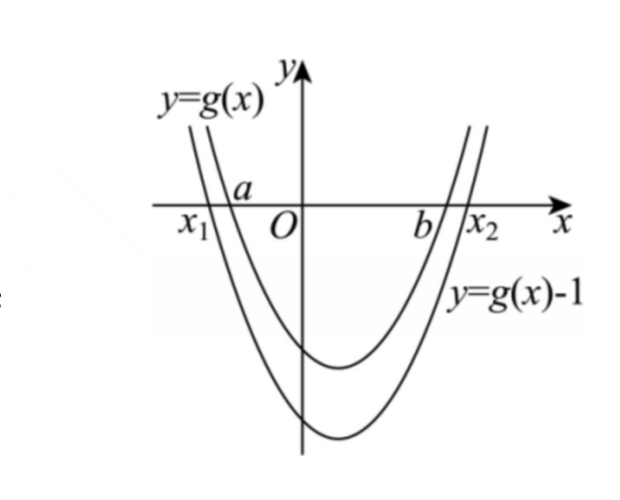
\includegraphics[width=0.20\textwidth]{figures/gao103_q16.png}
\end{center}
\step{由图像得 $x_1<a<b<x_2$．故选 $B$.}
\solend

\fi

\end{enumerate}

\bigsec{三、解答题}

\begin{enumerate}
\setcounter{enumi}{16}

\item 已知集合 $A=\{x\mid-3\leqslant x\leqslant1\}$，$B=\{x\mid a-2<x<a+2,a\in\R\}$.

（1）当 $a=1$ 时，求 $A\cap B$、$A\cup B$；

（2）若 $B\subseteq\overline A$，求 $a$ 的取值范围.

\ansspace*[8]

\ifanswer
\solbegin
\stepm{（1）}{当 $a=1$ 时，$B=\{x\mid-1<x<3\}$，又因为 $A=\{x\mid-3\leqslant x\leqslant1\}$，}
\step{所以 $A\cap B=\{x\mid-1<x\leqslant1\}$，$A\cup B=\{x\mid-3\leqslant x<3\}$；}
\stepm{（2）}{由 $A=\{x\mid-3\leqslant x\leqslant1\}$，得 $\overline A=\{x\mid x<-3\text{ 或 }x>1\}$，}
\step{若 $B\subseteq\overline A$，易得 $B=\{x\mid a-2<x<a+2,a\in\R\}\neq\varnothing$，}
\step{所以 $a+2\leqslant-3$ 或 $a-2\geqslant1$，解得 $a\leqslant-5$ 或 $a\geqslant3$，}
\step{综上所述，实数 $a$ 的取值范围是 $(-\infty,-5]\cup[3,+\infty)$.}
\solend

\fi

\item （1）解不等式 $\lvert 1-2x\rvert>x$；

（2）已知 $a$、$b$ 都是有理数，满足 $a+b\sqrt5=0$，请用反证法证明：$a=b=0$.

\ansspace*[10]

\ifanswer
\solbegin
\stepm{（1）}{①当 $x<0$ 时，左边非负，右边为负，不等式显然成立；}
\step{②当 $x\geqslant0$ 时，两边平方，$(1-2x)^2>x^2\Rightarrow3x^2-4x+1>0$}
\step{$\Rightarrow(3x-1)(x-1)>0$，解得 $x<\dfrac13$ 或 $x>1$，结合 $x\geqslant0$，}
\step{得 $0\leqslant x<\dfrac13$ 或 $x>1$；}
\step{综上，不等式解集为 $\left(-\infty,\dfrac13\right)\cup(1,+\infty)$.}
\stepm{（2）}{假设 $a,b$ 至少有一个不为零，}
\step{当 $a,b$ 中有一个为零一个不为零时，不妨设 $\begin{cases}a\neq0\\ b=0\end{cases}$，}
\step{则 $a+b\sqrt5=0\Rightarrow a=0$ 矛盾，舍；}
\step{当 $\begin{cases}a\neq0\\ b\neq0\end{cases}$ 时，$a+b\sqrt5=0\Rightarrow\sqrt5=-\dfrac ab\in\Q$，矛盾，舍，}
\step{综上假设不成立，所以 $a=b=0$.}
\solend

\fi

\item 某物流公司为了扩大业务量，计划建造一间高为 6 米，底面积为 24 平方米，且背面靠
墙的长方形形状的仓库。仓库的背面靠墙，无须建造费用，因此甲工程队给出的报价为：
仓库前面新建墙体每平方米 400 元，左右两面新建墙体每平方米 300 元，屋顶和地面以及
其他共计 28800 元.

（1）设仓库前面墙体的长为 $x$ 米 $(x>0)$，甲工程队的整体报价为 $y$ 元。若该物流公司计
划投入的改造资金不超过 60000 元，求前面墙体长 $x$ 的取值范围.

（2）在（1）的条件下，当仓库前面墙体的长度为多少时，甲工程队的整体
报价最低？

\begin{center}
% 原图第 7 页题干仓库示意图直接裁取（原卷排于题干右侧），已去粉色水印转灰度。
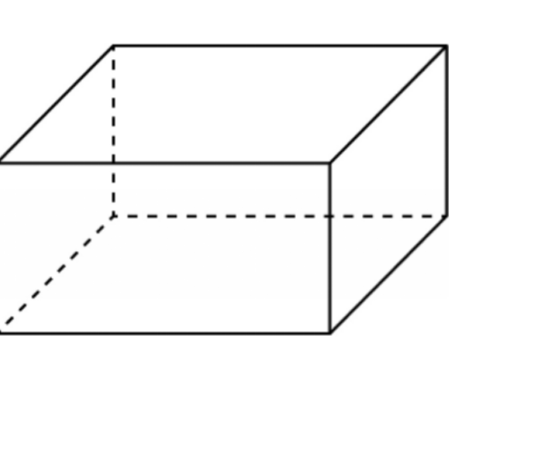
\includegraphics[width=0.17\textwidth]{figures/gao103_q19.png}
\end{center}

\ansspace*[12]

\ifanswer
\solbegin
\stepm{（1）}{甲队整体报价为 $y=400\times6x+2\times300\times6\times\dfrac{24}{x}+28800$}
\step{$=2400x+\dfrac{86400}{x}+28800$ 元，}
\step{要求 $y\leqslant60000$，即 $2400x+\dfrac{86400}{x}+28800\leqslant60000$，}
\step{化简得 $x+\dfrac{36}{x}\leqslant13$，}
\step{由于 $x>0$，则不等式化为 $x^2-13x+36\leqslant0$，}
\step{即 $(x-4)(x-9)\leqslant0$，解得 $4\leqslant x\leqslant9$，}
\step{所以前面墙体长 $x$ 的取值范围为 $[4,9]$；}
\stepm{（2）}{甲队整体报价为 $y=2400x+\dfrac{86400}{x}$}
\step{$\geqslant2\sqrt{2400x\times\dfrac{86400}{x}}+28800=57600$，}
\step{当且仅当 $2400x=\dfrac{86400}{x}$，即 $x^2=36$，}
\step{解得 $x=6$（满足 $4\leqslant x\leqslant9$）时取等号，}
\step{所以当仓库前面墙体的长度为 6 米时，甲工程队的整体报价最低，}
\step{为 57600 元.}
\solend

\fi

\item 已知函数 $f(x)=ax^2-10x+4b$.

（1）当 $a=1$，$b=4$ 时，解不等式 $f(x)\geqslant0$；

（2）若关于 $x$ 的不等式 $f(x)<0$ 的解集为 $(a,b)$，求实数 $a$、$b$ 的值；

（3）若 1 是 $f(x)$ 的零点，且 $a>0$，$b>0$，问当 $a$、$b$ 取何值时，$\dfrac1a+\dfrac1b$ 的值最小？最
小值是多少？

\ansspace*[12]

\ifanswer
\solbegin
\stepm{（1）}{将 $a=1$，$b=4$ 代入得 $f(x)=x^2-10x+16\geqslant0$，解得 $x\geqslant8$ 或 $x\leqslant2$，}
\step{所以不等式的解集为 $\{x\mid x\geqslant8\text{ 或 }x\leqslant2\}$；}
\stepm{（2）}{由题意得 $a$、$b$ 是 $ax^2-10x+4b=0$ 两根，且 $a<b$，$a>0$，}
\step{由韦达定理得 $\begin{cases}a+b=\dfrac{10}{a}\\ a\cdot b=\dfrac{4b}{a}\end{cases}$，解得 $\begin{cases}a=2\\ b=3\end{cases}$，即实数 $a$、$b$ 的值分别为 2，3；}
\stepm{（3）}{由 1 是 $f(x)$ 的零点，得 $f(1)=a-10+4b=0$，得 $a+4b=10$，}
\step{因为 $a>0$，$b>0$，}
\step{所以 $\dfrac1a+\dfrac1b=\dfrac1{10}\left(\dfrac1a+\dfrac1b\right)(a+4b)=\dfrac1{10}\left(1+4+\dfrac{4b}{a}+\dfrac ab\right)$}
\step{$\geqslant\dfrac1{10}\left(5+2\sqrt{\dfrac{4b}{a}\cdot\dfrac ab}\right)=\dfrac9{10}$，}
\step{当且仅当 $\dfrac{4b}{a}=\dfrac ab$，即 $a=\dfrac{10}3$,$b=\dfrac53$ 时取等号，}
\step{所以 $\dfrac1a+\dfrac1b$ 取最小值，且最小值为 $\dfrac9{10}$.}
\solend

\fi

\item 已知集合 $A$ 为非空集合，定义 $S=\{x\mid x=a+b,a,b\in A\}$，
$T=\{x\mid x=\lvert a-b\rvert,a,b\in A\}$.

（1）若集合 $A=\{1,3\}$，直接写出集合 $S$、$T$ (无需写计算过程)；

（2）若集合 $A=\{x_1,x_2,x_3,x_4\},x_1<x_2<x_3<x_4$，且 $T=A$，求证：$x_1+x_4=x_2+x_3$；

（3）若集合 $A=\{x\mid0\leqslant x\leqslant2026,x\in\N\}$,$S\cap T=\varnothing$．记 $\lvert A\rvert$ 为集合 $A$ 中元素的个数，求
$\lvert A\rvert$ 的最大值.

\ansspace*[16]

\ifanswer
\solbegin
\stepm{（1）}{$S=\{2,4,6\}$,$T=\{0,2\}$；}
\stepm{（2）}{集合 $T$ 中最小的元素为 0，因为 $T=A$，且 $x_1<x_2<x_3<x_4$，所以 $x_1=0$，}
\step{所以集合 $T$ 中元素为 $x_2-x_1=x_2$,$x_3-x_1=x_3$,$x_4-x_1=x_4$，}
\step{以及 $x_3-x_2$,$x_4-x_2$,$x_4-x_3$ 均属于 $A$，}
\step{因为 $x_1=0<x_3-x_2<x_4-x_2<x_4$，所以 $x_3$ 即 $x_4-x_2=x_3-x_1$，}
\step{即 $x_1+x_4=x_2+x_3$；}
\stepm{（3）}{设 $A=\{a_1,a_2,a_3,\cdots,a_k\}$ 满足题意，其中 $a_1<a_2<\cdots<a_k$，}
\step{则 $2a_1<a_1+a_2<\cdots<a_1+a_k<a_2+a_k<a_3+a_k<\cdots<a_{k-1}+a_k<2a_k$，}
\step{所以 $\lvert S\cup T\rvert\leqslant2k+1$，所以 $3k-1\leqslant2a_k+1\leqslant4053(k\in\N^*)$，}
\step{所以 $k\leqslant1351$，}
\step{实际上当 $A=\{676,677,\cdots,2026\}$ 时满足题意，}
\step{证明如下：设 $A=\{m,m+1,m+2,\cdots,2026\},m\in N$，}
\step{设 $S=\{2m,2m+1,2m+2,\cdots,4052\}$,$T=\{0,1,2,\cdots,2026-m\}$，}
\step{由题意得 $2026-m<2m$，即 $m>675\dfrac13$，}
\step{故 $m$ 的最小值是 676，于是当 $m=676$,$A$ 中的元素最多，}
\step{即 $A=\{676,677,\cdots,2026\}$ 时满足题意，}
\step{综上所述，集合 $A$ 中元素的个数的最大值是 1351.}
\solend

\fi

\end{enumerate}

\end{document}
"
%
% 原始材料：微信公众号“魔都数学加油站”文章，作者破晓，2026-11-01 21:56 发布；
% 连载“27学年高一103”，原文标题“27学年高一103——2026-2027年上海市市北中学高一上10月月考”；
% 原文链接：https://mp.weixin.qq.com/s/iBvF4eKw66F-kS6xLmDpBA。
% 正文为 10 张 PNG 页（第 1、3、5、6、7、10 页 2560×3620，其余 4762×6735），题目下印有【解析】，为讲评版。
% 题目、解析均据原图转录；卷面水印及公众号页脚未录入。
%
% 卷首标题：原卷印作“2026-2027 年市北中学高一上 10 月月考”（公众号标题中的“上海市”“高一上”
% 卷面标题行没有或已含，本稿照卷面），年份区间按全稿惯例排 en dash；原卷未印副标题，本稿按题目
% 内容标为“集合与常用逻辑用语、不等式”。
%
% 与原卷的排版差异：
%   ① 原文从第 3 题起，填空题编号为 3—12、选择题为 13—16、解答题为 17—21，本稿保留原题号；
%   ② 原卷每题下直接印【解析】，本稿按全稿惯例将解析置于答案版；选择题括号内未印答案，另由
%      解析末句“故选 X”给出；
%   ③ 原卷未印副标题，本稿按“知识模块”口径补出；
%   ④ 原卷填空横线按全稿惯例排为 \blankline[4.4em]；解答题按惯例加 \ansspace；选择题括号排
%      \mbox{（\quad）}；
%   ⑤ 原卷数集排斜体 $R$／$Q$（第 18 题解析 $Q$ 排粗体），按全稿惯例改 $\R$／$\Q$；
%   ⑥ 第 14 题四个文氏图选项按原图形状用 TikZ 重排；第 16、19 两题的插图裁自原图
%      （去粉色水印转灰度），第 19 题图属题干（三版都出），第 16 题图属解析（仅答案版显示）。
%
% 原卷存疑／笔误（均照录加注）：
%   第 9 题解析“故 $a+b=3b+b<0$”（$a=3b$ 代入应为 $4b$，原卷写作 $3b+b$，数值相同）；
%   第 21 题 (2) 解析“所以 $x_3$ 即 $x_4-x_2=x_3-x_1$”表述含糊（意为 $x_4-x_2$ 恰为 $T$ 中
%   介于 $x_2$ 与 $x_4$ 之间的元素 $x_3-x_1$）；
%   第 21 题 (3) 解析“所以 $|S\cup T|\leqslant2k+1$”（按上下文应为 $2a_k+1$，与后半句
%   $3k-1\leqslant2a_k+1$ 呼应），照录。
%
% 行数核对：逐题数 \step/\stepm 条数，合计 119 条（Q3：2；Q4：2；Q5：5；Q6：3；Q8：3；
% Q9：7；Q10：5；Q11：8；Q12：7；Q13：6；Q14：5；Q15：6；Q16：4；Q17：6；Q18：10；
% Q19：13；Q20：10；Q21：17），与原卷印刷行逐题相等。第 7 题只印【答案】，提 \ans{}，
% 不计入 \step 账。
%
\documentclass[a4paper,11pt]{article}
\usepackage{common}

\begin{document}

\examtitlest[3]{2026--2027 年市北中学高一上 10 月月考}{集合与常用逻辑用语、不等式}

\bigsec{一、填空题}

\begin{enumerate}
\setcounter{enumi}{2}

\item 已知实数 $x$ 满足 $\dfrac{7-x}{x+4}>0$，则 $x$ 的取值范围是\blankline[4.4em].

\ifanswer
\solbegin
\step{不等式 $\dfrac{7-x}{x+4}>0$ 可化为 $\dfrac{x-7}{x+4}<0$，等价于 $(x-7)(x+4)<0$，}
\step{解得 $-4<x<7$，所以 $x$ 的取值范围是 $\{x\mid-4<x<7\}$.}
\solend

\fi

\item 已知 $x_1$、$x_2$ 为方程 $2x^2+6x+3=0$ 的两个实数根，则 $\dfrac1{x_1}+\dfrac1{x_2}=$\blankline[4.4em].

\ifanswer
\solbegin
\step{由根与系数的关系得 $x_1+x_2=-\dfrac62=-3$，$x_1x_2=\dfrac32$，}
\step{则 $\dfrac1{x_1}+\dfrac1{x_2}=\dfrac{x_1+x_2}{x_1x_2}=-2$.}
\solend

\fi

\item 已知 $y=\lvert x-2\rvert+\lvert x-5\rvert$，$x\in\R$，则 $y$ 的最小值为\blankline[4.4em].

\ifanswer
\solbegin
\step{$y=\lvert x-2\rvert+\lvert x-5\rvert=\begin{cases}7-2x, & x<2\\ 3, & 2\leqslant x\leqslant5\\ 2x-7, & x>5\end{cases}$，}
\step{当 $x<2$ 时，$y>7-2\times2=3$；}
\step{当 $2\leqslant x\leqslant5$ 时，$y=3$；}
\step{当 $x>5$ 时，$y>2\times5-7=3$.}
\step{综上所述，$y$ 的最小值为 3.}
\solend

\fi

\item 对任意实数 $x$，等式 $ax^4+bx^3+cx^2+dx+e=x(x-2)(x^2+3)$ 恒成立，则
$b+c+d=$\blankline[4.4em].

\ifanswer
\solbegin
\step{因为 $ax^4+bx^3+cx^2+dx+e=x(x-2)(x^2+3)=(x^2-2x)(x^2+3)$}
\step{$=x^4-2x^3+3x^2-6x$，所以 $a=1$，$b=-2$，$c=3$，$d=-6$，$e=0$，}
\step{所以 $b+c+d=-2+3-6=-5$.}
\solend

\fi

\item 命题：“存在 $x\in(1,+\infty)$，使得 $ax^2+bx+c<0$”的否定形式是\blankline[4.4em].

\ifanswer
\ans{对于任意的 $x\in(1,+\infty)$，都有 $ax^2+bx+c\geqslant0$}
\fi

\item 已知集合 $A=\{x\mid mx^2-2x+1=0,x\in\R\}$ 有且仅有两个子集，则实数 $m=$\blankline[4.4em].

\ifanswer
\solbegin
\step{①当 $m=0$ 时，方程为 $-2x+1=0$，解得 $x=\dfrac12$，满足 $A=\left\{\dfrac12\right\}$ 仅有两个子集；}
\step{②当 $m\neq0$ 时，方程有两个相等实根，所以 $\Delta=4-4m=0$，解得 $m=1$；}
\step{所以实数 $m$ 的值为 0 或 1.}
\solend

\fi

\item 设 $a$、$b\in\R$，已知关于 $x$ 的不等式 $(a+b)x+(b-3a)<0$ 的解集为 $(2,+\infty)$，则不等式
$(a-2b)x+5b-a>0$ 的解集为\blankline[4.4em].

\ifanswer
\solbegin
\step{关于 $x$ 的不等式 $(a+b)x+(b-3a)<0$ 的解集为 $(2,+\infty)$，}
\step{得 $x=2$ 是 $(a+b)x+(b-3a)=0$ 的解，且 $a+b<0$，}
\step{所以 $2(a+b)+(b-3a)=0$，化简得 $a=3b$，故 $a+b=3b+b<0$，即 $b<0$，}
\step{将 $a=3b$ 代入 $(a-2b)x+5b-a>0$，}
\step{得不等式 $(a-2b)x+5b-a>0$ 即 $b(x+2)>0$，}
\step{两边都除以 $b$，得 $x+2<0$，解得 $x<-2$，}
\step{所以不等式 $(a-2b)x+5b-a>0$ 的解集为 $(-\infty,-2)$.}
\solend

\fi

\item 已知不等式 $\lvert x-a\rvert<1$ 成立的充分不必要条件是 $\dfrac12<x<\dfrac32$，则实数 $a$ 的取值范围
是\blankline[4.4em].

\ifanswer
\solbegin
\step{$\lvert x-a\rvert<1$，解得 $a-1<x<1+a$，}
\step{所以 $a-1<x<1+a$ 成立的充分不必要条件是 $\dfrac12<x<\dfrac32$，}
\step{故 $\left\{x\left|\dfrac12<x<\dfrac32\right.\right\}$ 是 $\{x\mid a-1<x<1+a\}$ 的真子集，}
\step{所以 $a-1\leqslant\dfrac12$ 且 $1+a\geqslant\dfrac32$（等号不同时成立），解得 $\dfrac12\leqslant a\leqslant\dfrac32$，}
\step{故实数 $a$ 的取值范围是 $\left[\dfrac12,\dfrac32\right]$.}
\solend

\fi

\item 定义 $A\nabla B=\left\{z\,\middle|\,z=xy+\dfrac xy,x\in A,y\in B\right\}$，设集合 $A=\{0,2\}$，$B=\{1,2\}$，$C=\{1\}$，
则集合 $(A\nabla B)\nabla C=$\blankline[4.4em].

\ifanswer
\solbegin
\step{当 $x=0$，$y=1$ 或 2 时，$z=xy+\dfrac xy=0$；}
\step{当 $x=2$，$y=1$ 时，$z=xy+\dfrac xy=4$；}
\step{当 $x=2$，$y=2$ 时，$z=xy+\dfrac xy=5$；}
\step{所以 $A\nabla B=\{0,4,5\}$；}
\step{当 $x=0$，$y=1$ 时，$z=xy+\dfrac xy=0$；}
\step{当 $x=4$，$y=1$ 时，$z=xy+\dfrac xy=8$；}
\step{当 $x=5$，$y=1$ 时，$z=xy+\dfrac xy=10$；}
\step{所以 $(A\nabla B)\nabla C=\{0,8,10\}$.}
\solend

\fi

\item 集合 $M=\{66,-11,23,10,911,-1,-18,100,0,\pi\}$ 有 10 个元素，设 $M$ 的所有非空子集为
$M_i\,(i=1,2,\cdots,1023)$，每一个 $M_i$ 中所有元素乘积为 $m_i\,(i=1,2,\cdots,1023)$，则
$m_1+m_2+m_3+\cdots+m_{1023}=$\blankline[4.4em].

\ifanswer
\solbegin
\step{因为 $M$ 的所有非空子集为 $M_i\,(i=1,2,\cdots,1023)$，这 1023 个子集分成以下几种情况：}
\step{①含 0 的子集有 512 个，这些子集均满足 $m_i=0$；}
\step{②不含 0，含 $-1$ 且还含有其它元素的子集有 255 个，}
\step{③不含 0，不含 $-1$ 但含有其它元素的子集有 255 个，}
\step{④只含 $-1$ 的子集一个 $\{-1\}$，满足 $m_i=-1$；}
\step{其中②③中的集合是一一对应的，且满足 $m_i$ 对应成相反数，}
\step{故 $m_1+m_2+m_3+\cdots+m_{1023}=512\times0+255\times0-1=-1$.}
\solend

\fi

\end{enumerate}

\bigsec{二、选择题}

\begin{enumerate}
\setcounter{enumi}{12}

\item 下列说法中，正确说法的个数是\mbox{（\quad）}

①联合国安理会常任理事国能组成一个集合；

②市北中学很喜欢足球的同学能组成一个集合；

③实数 $1,0,5,\dfrac12,\dfrac32,\dfrac64,\sqrt{\dfrac14}$ 组成的集合中有 6 个元素.

\keepwithprev
A. $0$\qquad\qquad B. $1$\qquad\qquad C. $2$\qquad\qquad D. $3$.

\ifanswer
\solbegin
\step{对于①，“联合国安理会常任理事国”满足集合的定义，故①正确；}
\step{对于②，“很喜欢”不满足集合的确定性，}
\step{市北中学很喜欢足球的同学不能组成一个集合，故②错误；}
\step{对于③，$\dfrac64=\dfrac32$，$\sqrt{\dfrac14}=\dfrac12$，由集合的元素互异性，集合中共有 5 个元素，}
\step{故③错误.}
\step{所以正确说法的个数是 1 个．故选 $B$.}
\solend

\fi

\item 已知全集 $U=\R$，集合 $A=\left\{x\,\middle|\,\dfrac{2x-8}{x-5}\leqslant1,x\in\N\right\}$，集合 $B=\{x\mid x^2-7x+12\leqslant0\}$，则
正确表示集合 $A$ 与集合 $B$ 关系的文氏图是\mbox{（\quad）}

\keepwithprev
\begin{center}
% 原卷四个文氏图选项按原图形状用 TikZ 重排。
\begin{tabular}{c@{\qquad\qquad}c}
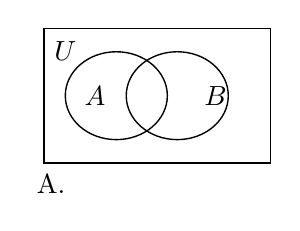
\begin{tikzpicture}[scale=0.9,line width=0.5pt]
\draw (0,0) rectangle (3.2,1.9);
\draw (1.02,0.95) ellipse (0.72 and 0.62);
\draw (1.88,0.95) ellipse (0.72 and 0.62);
\node at (0.72,0.95) {$A$};
\node at (2.42,0.95) {$B$};
\node at (0.3,1.58) {$U$};
\node[anchor=north] at (0.1,-0.03) {A.};
\end{tikzpicture}
&
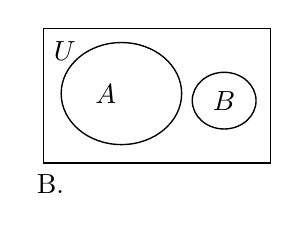
\begin{tikzpicture}[scale=0.9,line width=0.5pt]
\draw (0,0) rectangle (3.2,1.9);
\draw (1.1,0.98) ellipse (0.85 and 0.72);
\draw (2.55,0.88) ellipse (0.45 and 0.4);
\node at (0.88,0.98) {$A$};
\node at (2.55,0.88) {$B$};
\node at (0.3,1.58) {$U$};
\node[anchor=north] at (0.1,-0.03) {B.};
\end{tikzpicture}
\\[10pt]
\begin{tikzpicture}[scale=0.9,line width=0.5pt]
\draw (0,0) rectangle (3.2,1.9);
\draw (1.5,0.95) ellipse (0.98 and 0.8);
\draw (1.22,0.95) ellipse (0.44 and 0.38);
\node at (1.22,0.95) {$B$};
\node at (2.26,0.95) {$A$};
\node at (0.3,1.58) {$U$};
\node[anchor=north] at (0.1,-0.03) {C.};
\end{tikzpicture}
&
\begin{tikzpicture}[scale=0.9,line width=0.5pt]
\draw (0,0) rectangle (3.2,1.9);
\draw (1.5,0.95) ellipse (0.98 and 0.8);
\draw (1.28,0.95) ellipse (0.46 and 0.4);
\node at (1.28,0.95) {$A$};
\node at (2.3,0.95) {$B$};
\node at (0.3,1.58) {$U$};
\node[anchor=north] at (0.1,-0.03) {D.};
\end{tikzpicture}
\\
\end{tabular}
\end{center}

\ifanswer
\solbegin
\step{$\dfrac{2x-8}{x-5}\leqslant1\Rightarrow\dfrac{2x-8}{x-5}-1\leqslant0\Rightarrow\dfrac{x-3}{x-5}\leqslant0$，等价于 $\begin{cases}(x-3)(x-5)\leqslant0\\ x-5\neq0\end{cases}$，}
\step{解得 $3\leqslant x<5$，因为 $x\in\N$，所以 $A=\{3,4\}$，}
\step{解不等式 $x^2-7x+12\leqslant0$ 得 $B=\{x\mid3\leqslant x\leqslant4\}$，}
\step{集合 $A$ 中的元素 3，4 都属于集合 $B$，且 $B$ 中存在无数实数不属于 $A$，}
\step{所以 $A$ 是 $B$ 的真子集，$A$ 在 $B$ 内部．故选 $D$.}
\solend

\fi

\item 已知 $a$、$b$、$c\in\R$，则下列命题中真命题的个数是\mbox{（\quad）}

①若 $ac^2>bc^2$，则 $a>b$；②若 $\lvert a-2\rvert>\lvert b-2\rvert$，则 $(a-2)^2>(b-2)^2$；

③若 $a>b>c>0$，则 $\dfrac ab>\dfrac{a+c}{b+c}$；④若 $a>0$，$b>0$，$a+b>4$，$ab>4$，则 $a>2$，$b>2$.

\keepwithprev
A. $1$\qquad\qquad B. $2$\qquad\qquad C. $3$\qquad\qquad D. $4$

\ifanswer
\solbegin
\step{①若 $ac^2>bc^2$，则 $c^2>0$，则 $a>b$；所以①正确；}
\step{②若 $\lvert a-2\rvert>\lvert b-2\rvert$，则 $(a-2)^2>(b-2)^2$；满足不等式的基本性质，所以②正确；}
\step{③若 $a>b>c>0$，则 $\dfrac ab>\dfrac{a+c}{b+c}$；所以③正确；}
\step{④若 $a>0$，$b>0$，$a+b>4$，$ab>4$，则 $a>2$，$b>2$.}
\step{反例 $a=10$，$b=0.5$，满足条件，推不出结论，所以④不正确；}
\step{故选 $C$.}
\solend

\fi

\item 已知实数 $a<b$，关于 $x$ 的不等式 $x^2-(a+b)x+ab-1<0$ 的解集为 $(x_1,x_2)$，则实数
$a$、$b$、$x_1$、$x_2$ 从小到大的排列是\mbox{（\quad）}

\keepwithprev
A. $x_1<a<x_2<b$\qquad B. $x_1<a<b<x_2$\qquad C. $a<x_1<b<x_2$\qquad D. $a<x_1<x_2<b$

\ifanswer
\solbegin
\step{已知实数 $a<b$，关于 $x$ 的不等式 $x^2-(a+b)x+ab-1<0$ 的解集为 $(x_1,x_2)$，}
\step{因为 $x^2-(a+b)x+ab=(x-a)(x-b)$.}
\step{设函数 $g(x)=(x-a)(x-b)$，作函数 $g(x)$、$g(x)-1$ 的图象如下：}
\begin{center}
% 原图第 6 页解析插图直接裁取（原卷排于解析行右侧），已去粉色水印转灰度。
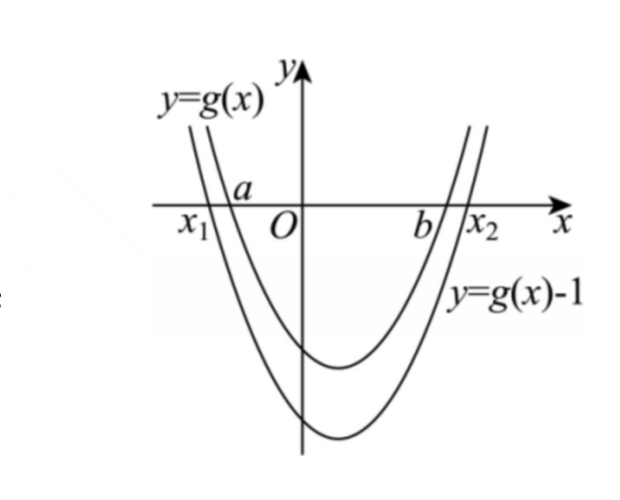
\includegraphics[width=0.20\textwidth]{figures/gao103_q16.png}
\end{center}
\step{由图像得 $x_1<a<b<x_2$．故选 $B$.}
\solend

\fi

\end{enumerate}

\bigsec{三、解答题}

\begin{enumerate}
\setcounter{enumi}{16}

\item 已知集合 $A=\{x\mid-3\leqslant x\leqslant1\}$，$B=\{x\mid a-2<x<a+2,a\in\R\}$.

（1）当 $a=1$ 时，求 $A\cap B$、$A\cup B$；

（2）若 $B\subseteq\overline A$，求 $a$ 的取值范围.

\ansspace*[8]

\ifanswer
\solbegin
\stepm{（1）}{当 $a=1$ 时，$B=\{x\mid-1<x<3\}$，又因为 $A=\{x\mid-3\leqslant x\leqslant1\}$，}
\step{所以 $A\cap B=\{x\mid-1<x\leqslant1\}$，$A\cup B=\{x\mid-3\leqslant x<3\}$；}
\stepm{（2）}{由 $A=\{x\mid-3\leqslant x\leqslant1\}$，得 $\overline A=\{x\mid x<-3\text{ 或 }x>1\}$，}
\step{若 $B\subseteq\overline A$，易得 $B=\{x\mid a-2<x<a+2,a\in\R\}\neq\varnothing$，}
\step{所以 $a+2\leqslant-3$ 或 $a-2\geqslant1$，解得 $a\leqslant-5$ 或 $a\geqslant3$，}
\step{综上所述，实数 $a$ 的取值范围是 $(-\infty,-5]\cup[3,+\infty)$.}
\solend

\fi

\item （1）解不等式 $\lvert 1-2x\rvert>x$；

（2）已知 $a$、$b$ 都是有理数，满足 $a+b\sqrt5=0$，请用反证法证明：$a=b=0$.

\ansspace*[10]

\ifanswer
\solbegin
\stepm{（1）}{①当 $x<0$ 时，左边非负，右边为负，不等式显然成立；}
\step{②当 $x\geqslant0$ 时，两边平方，$(1-2x)^2>x^2\Rightarrow3x^2-4x+1>0$}
\step{$\Rightarrow(3x-1)(x-1)>0$，解得 $x<\dfrac13$ 或 $x>1$，结合 $x\geqslant0$，}
\step{得 $0\leqslant x<\dfrac13$ 或 $x>1$；}
\step{综上，不等式解集为 $\left(-\infty,\dfrac13\right)\cup(1,+\infty)$.}
\stepm{（2）}{假设 $a,b$ 至少有一个不为零，}
\step{当 $a,b$ 中有一个为零一个不为零时，不妨设 $\begin{cases}a\neq0\\ b=0\end{cases}$，}
\step{则 $a+b\sqrt5=0\Rightarrow a=0$ 矛盾，舍；}
\step{当 $\begin{cases}a\neq0\\ b\neq0\end{cases}$ 时，$a+b\sqrt5=0\Rightarrow\sqrt5=-\dfrac ab\in\Q$，矛盾，舍，}
\step{综上假设不成立，所以 $a=b=0$.}
\solend

\fi

\item 某物流公司为了扩大业务量，计划建造一间高为 6 米，底面积为 24 平方米，且背面靠
墙的长方形形状的仓库。仓库的背面靠墙，无须建造费用，因此甲工程队给出的报价为：
仓库前面新建墙体每平方米 400 元，左右两面新建墙体每平方米 300 元，屋顶和地面以及
其他共计 28800 元.

（1）设仓库前面墙体的长为 $x$ 米 $(x>0)$，甲工程队的整体报价为 $y$ 元。若该物流公司计
划投入的改造资金不超过 60000 元，求前面墙体长 $x$ 的取值范围.

（2）在（1）的条件下，当仓库前面墙体的长度为多少时，甲工程队的整体
报价最低？

\begin{center}
% 原图第 7 页题干仓库示意图直接裁取（原卷排于题干右侧），已去粉色水印转灰度。
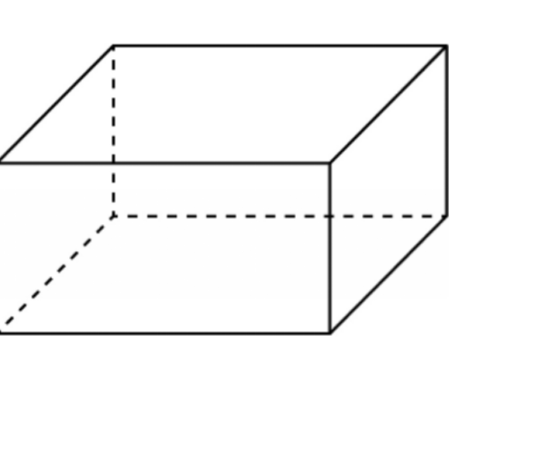
\includegraphics[width=0.17\textwidth]{figures/gao103_q19.png}
\end{center}

\ansspace*[12]

\ifanswer
\solbegin
\stepm{（1）}{甲队整体报价为 $y=400\times6x+2\times300\times6\times\dfrac{24}{x}+28800$}
\step{$=2400x+\dfrac{86400}{x}+28800$ 元，}
\step{要求 $y\leqslant60000$，即 $2400x+\dfrac{86400}{x}+28800\leqslant60000$，}
\step{化简得 $x+\dfrac{36}{x}\leqslant13$，}
\step{由于 $x>0$，则不等式化为 $x^2-13x+36\leqslant0$，}
\step{即 $(x-4)(x-9)\leqslant0$，解得 $4\leqslant x\leqslant9$，}
\step{所以前面墙体长 $x$ 的取值范围为 $[4,9]$；}
\stepm{（2）}{甲队整体报价为 $y=2400x+\dfrac{86400}{x}$}
\step{$\geqslant2\sqrt{2400x\times\dfrac{86400}{x}}+28800=57600$，}
\step{当且仅当 $2400x=\dfrac{86400}{x}$，即 $x^2=36$，}
\step{解得 $x=6$（满足 $4\leqslant x\leqslant9$）时取等号，}
\step{所以当仓库前面墙体的长度为 6 米时，甲工程队的整体报价最低，}
\step{为 57600 元.}
\solend

\fi

\item 已知函数 $f(x)=ax^2-10x+4b$.

（1）当 $a=1$，$b=4$ 时，解不等式 $f(x)\geqslant0$；

（2）若关于 $x$ 的不等式 $f(x)<0$ 的解集为 $(a,b)$，求实数 $a$、$b$ 的值；

（3）若 1 是 $f(x)$ 的零点，且 $a>0$，$b>0$，问当 $a$、$b$ 取何值时，$\dfrac1a+\dfrac1b$ 的值最小？最
小值是多少？

\ansspace*[12]

\ifanswer
\solbegin
\stepm{（1）}{将 $a=1$，$b=4$ 代入得 $f(x)=x^2-10x+16\geqslant0$，解得 $x\geqslant8$ 或 $x\leqslant2$，}
\step{所以不等式的解集为 $\{x\mid x\geqslant8\text{ 或 }x\leqslant2\}$；}
\stepm{（2）}{由题意得 $a$、$b$ 是 $ax^2-10x+4b=0$ 两根，且 $a<b$，$a>0$，}
\step{由韦达定理得 $\begin{cases}a+b=\dfrac{10}{a}\\ a\cdot b=\dfrac{4b}{a}\end{cases}$，解得 $\begin{cases}a=2\\ b=3\end{cases}$，即实数 $a$、$b$ 的值分别为 2，3；}
\stepm{（3）}{由 1 是 $f(x)$ 的零点，得 $f(1)=a-10+4b=0$，得 $a+4b=10$，}
\step{因为 $a>0$，$b>0$，}
\step{所以 $\dfrac1a+\dfrac1b=\dfrac1{10}\left(\dfrac1a+\dfrac1b\right)(a+4b)=\dfrac1{10}\left(1+4+\dfrac{4b}{a}+\dfrac ab\right)$}
\step{$\geqslant\dfrac1{10}\left(5+2\sqrt{\dfrac{4b}{a}\cdot\dfrac ab}\right)=\dfrac9{10}$，}
\step{当且仅当 $\dfrac{4b}{a}=\dfrac ab$，即 $a=\dfrac{10}3$,$b=\dfrac53$ 时取等号，}
\step{所以 $\dfrac1a+\dfrac1b$ 取最小值，且最小值为 $\dfrac9{10}$.}
\solend

\fi

\item 已知集合 $A$ 为非空集合，定义 $S=\{x\mid x=a+b,a,b\in A\}$，
$T=\{x\mid x=\lvert a-b\rvert,a,b\in A\}$.

（1）若集合 $A=\{1,3\}$，直接写出集合 $S$、$T$ (无需写计算过程)；

（2）若集合 $A=\{x_1,x_2,x_3,x_4\},x_1<x_2<x_3<x_4$，且 $T=A$，求证：$x_1+x_4=x_2+x_3$；

（3）若集合 $A=\{x\mid0\leqslant x\leqslant2026,x\in\N\}$,$S\cap T=\varnothing$．记 $\lvert A\rvert$ 为集合 $A$ 中元素的个数，求
$\lvert A\rvert$ 的最大值.

\ansspace*[16]

\ifanswer
\solbegin
\stepm{（1）}{$S=\{2,4,6\}$,$T=\{0,2\}$；}
\stepm{（2）}{集合 $T$ 中最小的元素为 0，因为 $T=A$，且 $x_1<x_2<x_3<x_4$，所以 $x_1=0$，}
\step{所以集合 $T$ 中元素为 $x_2-x_1=x_2$,$x_3-x_1=x_3$,$x_4-x_1=x_4$，}
\step{以及 $x_3-x_2$,$x_4-x_2$,$x_4-x_3$ 均属于 $A$，}
\step{因为 $x_1=0<x_3-x_2<x_4-x_2<x_4$，所以 $x_3$ 即 $x_4-x_2=x_3-x_1$，}
\step{即 $x_1+x_4=x_2+x_3$；}
\stepm{（3）}{设 $A=\{a_1,a_2,a_3,\cdots,a_k\}$ 满足题意，其中 $a_1<a_2<\cdots<a_k$，}
\step{则 $2a_1<a_1+a_2<\cdots<a_1+a_k<a_2+a_k<a_3+a_k<\cdots<a_{k-1}+a_k<2a_k$，}
\step{所以 $\lvert S\cup T\rvert\leqslant2k+1$，所以 $3k-1\leqslant2a_k+1\leqslant4053(k\in\N^*)$，}
\step{所以 $k\leqslant1351$，}
\step{实际上当 $A=\{676,677,\cdots,2026\}$ 时满足题意，}
\step{证明如下：设 $A=\{m,m+1,m+2,\cdots,2026\},m\in N$，}
\step{设 $S=\{2m,2m+1,2m+2,\cdots,4052\}$,$T=\{0,1,2,\cdots,2026-m\}$，}
\step{由题意得 $2026-m<2m$，即 $m>675\dfrac13$，}
\step{故 $m$ 的最小值是 676，于是当 $m=676$,$A$ 中的元素最多，}
\step{即 $A=\{676,677,\cdots,2026\}$ 时满足题意，}
\step{综上所述，集合 $A$ 中元素的个数的最大值是 1351.}
\solend

\fi

\end{enumerate}

\end{document}
"
%
% 原始材料：微信公众号“魔都数学加油站”文章，作者破晓，2026-11-01 21:56 发布；
% 连载“27学年高一103”，原文标题“27学年高一103——2026-2027年上海市市北中学高一上10月月考”；
% 原文链接：https://mp.weixin.qq.com/s/iBvF4eKw66F-kS6xLmDpBA。
% 正文为 10 张 PNG 页（第 1、3、5、6、7、10 页 2560×3620，其余 4762×6735），题目下印有【解析】，为讲评版。
% 题目、解析均据原图转录；卷面水印及公众号页脚未录入。
%
% 卷首标题：原卷印作“2026-2027 年市北中学高一上 10 月月考”（公众号标题中的“上海市”“高一上”
% 卷面标题行没有或已含，本稿照卷面），年份区间按全稿惯例排 en dash；原卷未印副标题，本稿按题目
% 内容标为“集合与常用逻辑用语、不等式”。
%
% 与原卷的排版差异：
%   ① 原文从第 3 题起，填空题编号为 3—12、选择题为 13—16、解答题为 17—21，本稿保留原题号；
%   ② 原卷每题下直接印【解析】，本稿按全稿惯例将解析置于答案版；选择题括号内未印答案，另由
%      解析末句“故选 X”给出；
%   ③ 原卷未印副标题，本稿按“知识模块”口径补出；
%   ④ 原卷填空横线按全稿惯例排为 \blankline[4.4em]；解答题按惯例加 \ansspace；选择题括号排
%      \mbox{（\quad）}；
%   ⑤ 原卷数集排斜体 $R$／$Q$（第 18 题解析 $Q$ 排粗体），按全稿惯例改 $\R$／$\Q$；
%   ⑥ 第 14 题四个文氏图选项按原图形状用 TikZ 重排；第 16、19 两题的插图裁自原图
%      （去粉色水印转灰度），第 19 题图属题干（三版都出），第 16 题图属解析（仅答案版显示）。
%
% 原卷存疑／笔误（均照录加注）：
%   第 9 题解析“故 $a+b=3b+b<0$”（$a=3b$ 代入应为 $4b$，原卷写作 $3b+b$，数值相同）；
%   第 21 题 (2) 解析“所以 $x_3$ 即 $x_4-x_2=x_3-x_1$”表述含糊（意为 $x_4-x_2$ 恰为 $T$ 中
%   介于 $x_2$ 与 $x_4$ 之间的元素 $x_3-x_1$）；
%   第 21 题 (3) 解析“所以 $|S\cup T|\leqslant2k+1$”（按上下文应为 $2a_k+1$，与后半句
%   $3k-1\leqslant2a_k+1$ 呼应），照录。
%
% 行数核对：逐题数 \step/\stepm 条数，合计 119 条（Q3：2；Q4：2；Q5：5；Q6：3；Q8：3；
% Q9：7；Q10：5；Q11：8；Q12：7；Q13：6；Q14：5；Q15：6；Q16：4；Q17：6；Q18：10；
% Q19：13；Q20：10；Q21：17），与原卷印刷行逐题相等。第 7 题只印【答案】，提 \ans{}，
% 不计入 \step 账。
%
\documentclass[a4paper,11pt]{article}
\usepackage{common}

\begin{document}

\examtitlest[3]{2026--2027 年市北中学高一上 10 月月考}{集合与常用逻辑用语、不等式}

\bigsec{一、填空题}

\begin{enumerate}
\setcounter{enumi}{2}

\item 已知实数 $x$ 满足 $\dfrac{7-x}{x+4}>0$，则 $x$ 的取值范围是\blankline[4.4em].

\ifanswer
\solbegin
\step{不等式 $\dfrac{7-x}{x+4}>0$ 可化为 $\dfrac{x-7}{x+4}<0$，等价于 $(x-7)(x+4)<0$，}
\step{解得 $-4<x<7$，所以 $x$ 的取值范围是 $\{x\mid-4<x<7\}$.}
\solend

\fi

\item 已知 $x_1$、$x_2$ 为方程 $2x^2+6x+3=0$ 的两个实数根，则 $\dfrac1{x_1}+\dfrac1{x_2}=$\blankline[4.4em].

\ifanswer
\solbegin
\step{由根与系数的关系得 $x_1+x_2=-\dfrac62=-3$，$x_1x_2=\dfrac32$，}
\step{则 $\dfrac1{x_1}+\dfrac1{x_2}=\dfrac{x_1+x_2}{x_1x_2}=-2$.}
\solend

\fi

\item 已知 $y=\lvert x-2\rvert+\lvert x-5\rvert$，$x\in\R$，则 $y$ 的最小值为\blankline[4.4em].

\ifanswer
\solbegin
\step{$y=\lvert x-2\rvert+\lvert x-5\rvert=\begin{cases}7-2x, & x<2\\ 3, & 2\leqslant x\leqslant5\\ 2x-7, & x>5\end{cases}$，}
\step{当 $x<2$ 时，$y>7-2\times2=3$；}
\step{当 $2\leqslant x\leqslant5$ 时，$y=3$；}
\step{当 $x>5$ 时，$y>2\times5-7=3$.}
\step{综上所述，$y$ 的最小值为 3.}
\solend

\fi

\item 对任意实数 $x$，等式 $ax^4+bx^3+cx^2+dx+e=x(x-2)(x^2+3)$ 恒成立，则
$b+c+d=$\blankline[4.4em].

\ifanswer
\solbegin
\step{因为 $ax^4+bx^3+cx^2+dx+e=x(x-2)(x^2+3)=(x^2-2x)(x^2+3)$}
\step{$=x^4-2x^3+3x^2-6x$，所以 $a=1$，$b=-2$，$c=3$，$d=-6$，$e=0$，}
\step{所以 $b+c+d=-2+3-6=-5$.}
\solend

\fi

\item 命题：“存在 $x\in(1,+\infty)$，使得 $ax^2+bx+c<0$”的否定形式是\blankline[4.4em].

\ifanswer
\ans{对于任意的 $x\in(1,+\infty)$，都有 $ax^2+bx+c\geqslant0$}
\fi

\item 已知集合 $A=\{x\mid mx^2-2x+1=0,x\in\R\}$ 有且仅有两个子集，则实数 $m=$\blankline[4.4em].

\ifanswer
\solbegin
\step{①当 $m=0$ 时，方程为 $-2x+1=0$，解得 $x=\dfrac12$，满足 $A=\left\{\dfrac12\right\}$ 仅有两个子集；}
\step{②当 $m\neq0$ 时，方程有两个相等实根，所以 $\Delta=4-4m=0$，解得 $m=1$；}
\step{所以实数 $m$ 的值为 0 或 1.}
\solend

\fi

\item 设 $a$、$b\in\R$，已知关于 $x$ 的不等式 $(a+b)x+(b-3a)<0$ 的解集为 $(2,+\infty)$，则不等式
$(a-2b)x+5b-a>0$ 的解集为\blankline[4.4em].

\ifanswer
\solbegin
\step{关于 $x$ 的不等式 $(a+b)x+(b-3a)<0$ 的解集为 $(2,+\infty)$，}
\step{得 $x=2$ 是 $(a+b)x+(b-3a)=0$ 的解，且 $a+b<0$，}
\step{所以 $2(a+b)+(b-3a)=0$，化简得 $a=3b$，故 $a+b=3b+b<0$，即 $b<0$，}
\step{将 $a=3b$ 代入 $(a-2b)x+5b-a>0$，}
\step{得不等式 $(a-2b)x+5b-a>0$ 即 $b(x+2)>0$，}
\step{两边都除以 $b$，得 $x+2<0$，解得 $x<-2$，}
\step{所以不等式 $(a-2b)x+5b-a>0$ 的解集为 $(-\infty,-2)$.}
\solend

\fi

\item 已知不等式 $\lvert x-a\rvert<1$ 成立的充分不必要条件是 $\dfrac12<x<\dfrac32$，则实数 $a$ 的取值范围
是\blankline[4.4em].

\ifanswer
\solbegin
\step{$\lvert x-a\rvert<1$，解得 $a-1<x<1+a$，}
\step{所以 $a-1<x<1+a$ 成立的充分不必要条件是 $\dfrac12<x<\dfrac32$，}
\step{故 $\left\{x\left|\dfrac12<x<\dfrac32\right.\right\}$ 是 $\{x\mid a-1<x<1+a\}$ 的真子集，}
\step{所以 $a-1\leqslant\dfrac12$ 且 $1+a\geqslant\dfrac32$（等号不同时成立），解得 $\dfrac12\leqslant a\leqslant\dfrac32$，}
\step{故实数 $a$ 的取值范围是 $\left[\dfrac12,\dfrac32\right]$.}
\solend

\fi

\item 定义 $A\nabla B=\left\{z\,\middle|\,z=xy+\dfrac xy,x\in A,y\in B\right\}$，设集合 $A=\{0,2\}$，$B=\{1,2\}$，$C=\{1\}$，
则集合 $(A\nabla B)\nabla C=$\blankline[4.4em].

\ifanswer
\solbegin
\step{当 $x=0$，$y=1$ 或 2 时，$z=xy+\dfrac xy=0$；}
\step{当 $x=2$，$y=1$ 时，$z=xy+\dfrac xy=4$；}
\step{当 $x=2$，$y=2$ 时，$z=xy+\dfrac xy=5$；}
\step{所以 $A\nabla B=\{0,4,5\}$；}
\step{当 $x=0$，$y=1$ 时，$z=xy+\dfrac xy=0$；}
\step{当 $x=4$，$y=1$ 时，$z=xy+\dfrac xy=8$；}
\step{当 $x=5$，$y=1$ 时，$z=xy+\dfrac xy=10$；}
\step{所以 $(A\nabla B)\nabla C=\{0,8,10\}$.}
\solend

\fi

\item 集合 $M=\{66,-11,23,10,911,-1,-18,100,0,\pi\}$ 有 10 个元素，设 $M$ 的所有非空子集为
$M_i\,(i=1,2,\cdots,1023)$，每一个 $M_i$ 中所有元素乘积为 $m_i\,(i=1,2,\cdots,1023)$，则
$m_1+m_2+m_3+\cdots+m_{1023}=$\blankline[4.4em].

\ifanswer
\solbegin
\step{因为 $M$ 的所有非空子集为 $M_i\,(i=1,2,\cdots,1023)$，这 1023 个子集分成以下几种情况：}
\step{①含 0 的子集有 512 个，这些子集均满足 $m_i=0$；}
\step{②不含 0，含 $-1$ 且还含有其它元素的子集有 255 个，}
\step{③不含 0，不含 $-1$ 但含有其它元素的子集有 255 个，}
\step{④只含 $-1$ 的子集一个 $\{-1\}$，满足 $m_i=-1$；}
\step{其中②③中的集合是一一对应的，且满足 $m_i$ 对应成相反数，}
\step{故 $m_1+m_2+m_3+\cdots+m_{1023}=512\times0+255\times0-1=-1$.}
\solend

\fi

\end{enumerate}

\bigsec{二、选择题}

\begin{enumerate}
\setcounter{enumi}{12}

\item 下列说法中，正确说法的个数是\mbox{（\quad）}

①联合国安理会常任理事国能组成一个集合；

②市北中学很喜欢足球的同学能组成一个集合；

③实数 $1,0,5,\dfrac12,\dfrac32,\dfrac64,\sqrt{\dfrac14}$ 组成的集合中有 6 个元素.

\keepwithprev
A. $0$\qquad\qquad B. $1$\qquad\qquad C. $2$\qquad\qquad D. $3$.

\ifanswer
\solbegin
\step{对于①，“联合国安理会常任理事国”满足集合的定义，故①正确；}
\step{对于②，“很喜欢”不满足集合的确定性，}
\step{市北中学很喜欢足球的同学不能组成一个集合，故②错误；}
\step{对于③，$\dfrac64=\dfrac32$，$\sqrt{\dfrac14}=\dfrac12$，由集合的元素互异性，集合中共有 5 个元素，}
\step{故③错误.}
\step{所以正确说法的个数是 1 个．故选 $B$.}
\solend

\fi

\item 已知全集 $U=\R$，集合 $A=\left\{x\,\middle|\,\dfrac{2x-8}{x-5}\leqslant1,x\in\N\right\}$，集合 $B=\{x\mid x^2-7x+12\leqslant0\}$，则
正确表示集合 $A$ 与集合 $B$ 关系的文氏图是\mbox{（\quad）}

\keepwithprev
\begin{center}
% 原卷四个文氏图选项按原图形状用 TikZ 重排。
\begin{tabular}{c@{\qquad\qquad}c}
\begin{tikzpicture}[scale=0.9,line width=0.5pt]
\draw (0,0) rectangle (3.2,1.9);
\draw (1.02,0.95) ellipse (0.72 and 0.62);
\draw (1.88,0.95) ellipse (0.72 and 0.62);
\node at (0.72,0.95) {$A$};
\node at (2.42,0.95) {$B$};
\node at (0.3,1.58) {$U$};
\node[anchor=north] at (0.1,-0.03) {A.};
\end{tikzpicture}
&
\begin{tikzpicture}[scale=0.9,line width=0.5pt]
\draw (0,0) rectangle (3.2,1.9);
\draw (1.1,0.98) ellipse (0.85 and 0.72);
\draw (2.55,0.88) ellipse (0.45 and 0.4);
\node at (0.88,0.98) {$A$};
\node at (2.55,0.88) {$B$};
\node at (0.3,1.58) {$U$};
\node[anchor=north] at (0.1,-0.03) {B.};
\end{tikzpicture}
\\[10pt]
\begin{tikzpicture}[scale=0.9,line width=0.5pt]
\draw (0,0) rectangle (3.2,1.9);
\draw (1.5,0.95) ellipse (0.98 and 0.8);
\draw (1.22,0.95) ellipse (0.44 and 0.38);
\node at (1.22,0.95) {$B$};
\node at (2.26,0.95) {$A$};
\node at (0.3,1.58) {$U$};
\node[anchor=north] at (0.1,-0.03) {C.};
\end{tikzpicture}
&
\begin{tikzpicture}[scale=0.9,line width=0.5pt]
\draw (0,0) rectangle (3.2,1.9);
\draw (1.5,0.95) ellipse (0.98 and 0.8);
\draw (1.28,0.95) ellipse (0.46 and 0.4);
\node at (1.28,0.95) {$A$};
\node at (2.3,0.95) {$B$};
\node at (0.3,1.58) {$U$};
\node[anchor=north] at (0.1,-0.03) {D.};
\end{tikzpicture}
\\
\end{tabular}
\end{center}

\ifanswer
\solbegin
\step{$\dfrac{2x-8}{x-5}\leqslant1\Rightarrow\dfrac{2x-8}{x-5}-1\leqslant0\Rightarrow\dfrac{x-3}{x-5}\leqslant0$，等价于 $\begin{cases}(x-3)(x-5)\leqslant0\\ x-5\neq0\end{cases}$，}
\step{解得 $3\leqslant x<5$，因为 $x\in\N$，所以 $A=\{3,4\}$，}
\step{解不等式 $x^2-7x+12\leqslant0$ 得 $B=\{x\mid3\leqslant x\leqslant4\}$，}
\step{集合 $A$ 中的元素 3，4 都属于集合 $B$，且 $B$ 中存在无数实数不属于 $A$，}
\step{所以 $A$ 是 $B$ 的真子集，$A$ 在 $B$ 内部．故选 $D$.}
\solend

\fi

\item 已知 $a$、$b$、$c\in\R$，则下列命题中真命题的个数是\mbox{（\quad）}

①若 $ac^2>bc^2$，则 $a>b$；②若 $\lvert a-2\rvert>\lvert b-2\rvert$，则 $(a-2)^2>(b-2)^2$；

③若 $a>b>c>0$，则 $\dfrac ab>\dfrac{a+c}{b+c}$；④若 $a>0$，$b>0$，$a+b>4$，$ab>4$，则 $a>2$，$b>2$.

\keepwithprev
A. $1$\qquad\qquad B. $2$\qquad\qquad C. $3$\qquad\qquad D. $4$

\ifanswer
\solbegin
\step{①若 $ac^2>bc^2$，则 $c^2>0$，则 $a>b$；所以①正确；}
\step{②若 $\lvert a-2\rvert>\lvert b-2\rvert$，则 $(a-2)^2>(b-2)^2$；满足不等式的基本性质，所以②正确；}
\step{③若 $a>b>c>0$，则 $\dfrac ab>\dfrac{a+c}{b+c}$；所以③正确；}
\step{④若 $a>0$，$b>0$，$a+b>4$，$ab>4$，则 $a>2$，$b>2$.}
\step{反例 $a=10$，$b=0.5$，满足条件，推不出结论，所以④不正确；}
\step{故选 $C$.}
\solend

\fi

\item 已知实数 $a<b$，关于 $x$ 的不等式 $x^2-(a+b)x+ab-1<0$ 的解集为 $(x_1,x_2)$，则实数
$a$、$b$、$x_1$、$x_2$ 从小到大的排列是\mbox{（\quad）}

\keepwithprev
A. $x_1<a<x_2<b$\qquad B. $x_1<a<b<x_2$\qquad C. $a<x_1<b<x_2$\qquad D. $a<x_1<x_2<b$

\ifanswer
\solbegin
\step{已知实数 $a<b$，关于 $x$ 的不等式 $x^2-(a+b)x+ab-1<0$ 的解集为 $(x_1,x_2)$，}
\step{因为 $x^2-(a+b)x+ab=(x-a)(x-b)$.}
\step{设函数 $g(x)=(x-a)(x-b)$，作函数 $g(x)$、$g(x)-1$ 的图象如下：}
\begin{center}
% 原图第 6 页解析插图直接裁取（原卷排于解析行右侧），已去粉色水印转灰度。
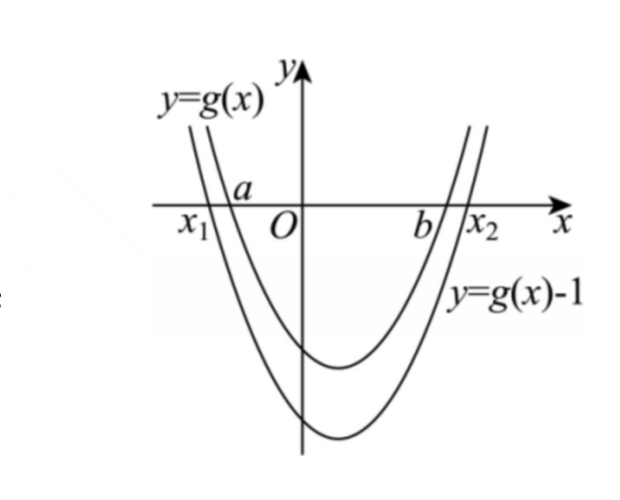
\includegraphics[width=0.20\textwidth]{figures/gao103_q16.png}
\end{center}
\step{由图像得 $x_1<a<b<x_2$．故选 $B$.}
\solend

\fi

\end{enumerate}

\bigsec{三、解答题}

\begin{enumerate}
\setcounter{enumi}{16}

\item 已知集合 $A=\{x\mid-3\leqslant x\leqslant1\}$，$B=\{x\mid a-2<x<a+2,a\in\R\}$.

（1）当 $a=1$ 时，求 $A\cap B$、$A\cup B$；

（2）若 $B\subseteq\overline A$，求 $a$ 的取值范围.

\ansspace*[8]

\ifanswer
\solbegin
\stepm{（1）}{当 $a=1$ 时，$B=\{x\mid-1<x<3\}$，又因为 $A=\{x\mid-3\leqslant x\leqslant1\}$，}
\step{所以 $A\cap B=\{x\mid-1<x\leqslant1\}$，$A\cup B=\{x\mid-3\leqslant x<3\}$；}
\stepm{（2）}{由 $A=\{x\mid-3\leqslant x\leqslant1\}$，得 $\overline A=\{x\mid x<-3\text{ 或 }x>1\}$，}
\step{若 $B\subseteq\overline A$，易得 $B=\{x\mid a-2<x<a+2,a\in\R\}\neq\varnothing$，}
\step{所以 $a+2\leqslant-3$ 或 $a-2\geqslant1$，解得 $a\leqslant-5$ 或 $a\geqslant3$，}
\step{综上所述，实数 $a$ 的取值范围是 $(-\infty,-5]\cup[3,+\infty)$.}
\solend

\fi

\item （1）解不等式 $\lvert 1-2x\rvert>x$；

（2）已知 $a$、$b$ 都是有理数，满足 $a+b\sqrt5=0$，请用反证法证明：$a=b=0$.

\ansspace*[10]

\ifanswer
\solbegin
\stepm{（1）}{①当 $x<0$ 时，左边非负，右边为负，不等式显然成立；}
\step{②当 $x\geqslant0$ 时，两边平方，$(1-2x)^2>x^2\Rightarrow3x^2-4x+1>0$}
\step{$\Rightarrow(3x-1)(x-1)>0$，解得 $x<\dfrac13$ 或 $x>1$，结合 $x\geqslant0$，}
\step{得 $0\leqslant x<\dfrac13$ 或 $x>1$；}
\step{综上，不等式解集为 $\left(-\infty,\dfrac13\right)\cup(1,+\infty)$.}
\stepm{（2）}{假设 $a,b$ 至少有一个不为零，}
\step{当 $a,b$ 中有一个为零一个不为零时，不妨设 $\begin{cases}a\neq0\\ b=0\end{cases}$，}
\step{则 $a+b\sqrt5=0\Rightarrow a=0$ 矛盾，舍；}
\step{当 $\begin{cases}a\neq0\\ b\neq0\end{cases}$ 时，$a+b\sqrt5=0\Rightarrow\sqrt5=-\dfrac ab\in\Q$，矛盾，舍，}
\step{综上假设不成立，所以 $a=b=0$.}
\solend

\fi

\item 某物流公司为了扩大业务量，计划建造一间高为 6 米，底面积为 24 平方米，且背面靠
墙的长方形形状的仓库。仓库的背面靠墙，无须建造费用，因此甲工程队给出的报价为：
仓库前面新建墙体每平方米 400 元，左右两面新建墙体每平方米 300 元，屋顶和地面以及
其他共计 28800 元.

（1）设仓库前面墙体的长为 $x$ 米 $(x>0)$，甲工程队的整体报价为 $y$ 元。若该物流公司计
划投入的改造资金不超过 60000 元，求前面墙体长 $x$ 的取值范围.

（2）在（1）的条件下，当仓库前面墙体的长度为多少时，甲工程队的整体
报价最低？

\begin{center}
% 原图第 7 页题干仓库示意图直接裁取（原卷排于题干右侧），已去粉色水印转灰度。
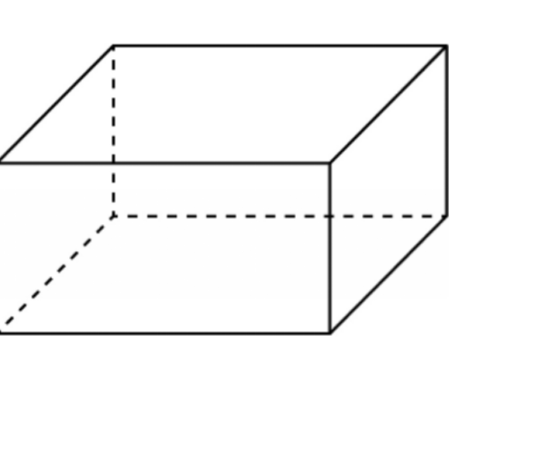
\includegraphics[width=0.17\textwidth]{figures/gao103_q19.png}
\end{center}

\ansspace*[12]

\ifanswer
\solbegin
\stepm{（1）}{甲队整体报价为 $y=400\times6x+2\times300\times6\times\dfrac{24}{x}+28800$}
\step{$=2400x+\dfrac{86400}{x}+28800$ 元，}
\step{要求 $y\leqslant60000$，即 $2400x+\dfrac{86400}{x}+28800\leqslant60000$，}
\step{化简得 $x+\dfrac{36}{x}\leqslant13$，}
\step{由于 $x>0$，则不等式化为 $x^2-13x+36\leqslant0$，}
\step{即 $(x-4)(x-9)\leqslant0$，解得 $4\leqslant x\leqslant9$，}
\step{所以前面墙体长 $x$ 的取值范围为 $[4,9]$；}
\stepm{（2）}{甲队整体报价为 $y=2400x+\dfrac{86400}{x}$}
\step{$\geqslant2\sqrt{2400x\times\dfrac{86400}{x}}+28800=57600$，}
\step{当且仅当 $2400x=\dfrac{86400}{x}$，即 $x^2=36$，}
\step{解得 $x=6$（满足 $4\leqslant x\leqslant9$）时取等号，}
\step{所以当仓库前面墙体的长度为 6 米时，甲工程队的整体报价最低，}
\step{为 57600 元.}
\solend

\fi

\item 已知函数 $f(x)=ax^2-10x+4b$.

（1）当 $a=1$，$b=4$ 时，解不等式 $f(x)\geqslant0$；

（2）若关于 $x$ 的不等式 $f(x)<0$ 的解集为 $(a,b)$，求实数 $a$、$b$ 的值；

（3）若 1 是 $f(x)$ 的零点，且 $a>0$，$b>0$，问当 $a$、$b$ 取何值时，$\dfrac1a+\dfrac1b$ 的值最小？最
小值是多少？

\ansspace*[12]

\ifanswer
\solbegin
\stepm{（1）}{将 $a=1$，$b=4$ 代入得 $f(x)=x^2-10x+16\geqslant0$，解得 $x\geqslant8$ 或 $x\leqslant2$，}
\step{所以不等式的解集为 $\{x\mid x\geqslant8\text{ 或 }x\leqslant2\}$；}
\stepm{（2）}{由题意得 $a$、$b$ 是 $ax^2-10x+4b=0$ 两根，且 $a<b$，$a>0$，}
\step{由韦达定理得 $\begin{cases}a+b=\dfrac{10}{a}\\ a\cdot b=\dfrac{4b}{a}\end{cases}$，解得 $\begin{cases}a=2\\ b=3\end{cases}$，即实数 $a$、$b$ 的值分别为 2，3；}
\stepm{（3）}{由 1 是 $f(x)$ 的零点，得 $f(1)=a-10+4b=0$，得 $a+4b=10$，}
\step{因为 $a>0$，$b>0$，}
\step{所以 $\dfrac1a+\dfrac1b=\dfrac1{10}\left(\dfrac1a+\dfrac1b\right)(a+4b)=\dfrac1{10}\left(1+4+\dfrac{4b}{a}+\dfrac ab\right)$}
\step{$\geqslant\dfrac1{10}\left(5+2\sqrt{\dfrac{4b}{a}\cdot\dfrac ab}\right)=\dfrac9{10}$，}
\step{当且仅当 $\dfrac{4b}{a}=\dfrac ab$，即 $a=\dfrac{10}3$,$b=\dfrac53$ 时取等号，}
\step{所以 $\dfrac1a+\dfrac1b$ 取最小值，且最小值为 $\dfrac9{10}$.}
\solend

\fi

\item 已知集合 $A$ 为非空集合，定义 $S=\{x\mid x=a+b,a,b\in A\}$，
$T=\{x\mid x=\lvert a-b\rvert,a,b\in A\}$.

（1）若集合 $A=\{1,3\}$，直接写出集合 $S$、$T$ (无需写计算过程)；

（2）若集合 $A=\{x_1,x_2,x_3,x_4\},x_1<x_2<x_3<x_4$，且 $T=A$，求证：$x_1+x_4=x_2+x_3$；

（3）若集合 $A=\{x\mid0\leqslant x\leqslant2026,x\in\N\}$,$S\cap T=\varnothing$．记 $\lvert A\rvert$ 为集合 $A$ 中元素的个数，求
$\lvert A\rvert$ 的最大值.

\ansspace*[16]

\ifanswer
\solbegin
\stepm{（1）}{$S=\{2,4,6\}$,$T=\{0,2\}$；}
\stepm{（2）}{集合 $T$ 中最小的元素为 0，因为 $T=A$，且 $x_1<x_2<x_3<x_4$，所以 $x_1=0$，}
\step{所以集合 $T$ 中元素为 $x_2-x_1=x_2$,$x_3-x_1=x_3$,$x_4-x_1=x_4$，}
\step{以及 $x_3-x_2$,$x_4-x_2$,$x_4-x_3$ 均属于 $A$，}
\step{因为 $x_1=0<x_3-x_2<x_4-x_2<x_4$，所以 $x_3$ 即 $x_4-x_2=x_3-x_1$，}
\step{即 $x_1+x_4=x_2+x_3$；}
\stepm{（3）}{设 $A=\{a_1,a_2,a_3,\cdots,a_k\}$ 满足题意，其中 $a_1<a_2<\cdots<a_k$，}
\step{则 $2a_1<a_1+a_2<\cdots<a_1+a_k<a_2+a_k<a_3+a_k<\cdots<a_{k-1}+a_k<2a_k$，}
\step{所以 $\lvert S\cup T\rvert\leqslant2k+1$，所以 $3k-1\leqslant2a_k+1\leqslant4053(k\in\N^*)$，}
\step{所以 $k\leqslant1351$，}
\step{实际上当 $A=\{676,677,\cdots,2026\}$ 时满足题意，}
\step{证明如下：设 $A=\{m,m+1,m+2,\cdots,2026\},m\in N$，}
\step{设 $S=\{2m,2m+1,2m+2,\cdots,4052\}$,$T=\{0,1,2,\cdots,2026-m\}$，}
\step{由题意得 $2026-m<2m$，即 $m>675\dfrac13$，}
\step{故 $m$ 的最小值是 676，于是当 $m=676$,$A$ 中的元素最多，}
\step{即 $A=\{676,677,\cdots,2026\}$ 时满足题意，}
\step{综上所述，集合 $A$ 中元素的个数的最大值是 1351.}
\solend

\fi

\end{enumerate}

\end{document}
"
%
% 原始材料：微信公众号“魔都数学加油站”文章，作者破晓，2026-11-01 21:56 发布；
% 连载“27学年高一103”，原文标题“27学年高一103——2026-2027年上海市市北中学高一上10月月考”；
% 原文链接：https://mp.weixin.qq.com/s/iBvF4eKw66F-kS6xLmDpBA。
% 正文为 10 张 PNG 页（第 1、3、5、6、7、10 页 2560×3620，其余 4762×6735），题目下印有【解析】，为讲评版。
% 题目、解析均据原图转录；卷面水印及公众号页脚未录入。
%
% 卷首标题：原卷印作“2026-2027 年市北中学高一上 10 月月考”（公众号标题中的“上海市”“高一上”
% 卷面标题行没有或已含，本稿照卷面），年份区间按全稿惯例排 en dash；原卷未印副标题，本稿按题目
% 内容标为“集合与常用逻辑用语、不等式”。
%
% 与原卷的排版差异：
%   ① 原文从第 3 题起，填空题编号为 3—12、选择题为 13—16、解答题为 17—21，本稿保留原题号；
%   ② 原卷每题下直接印【解析】，本稿按全稿惯例将解析置于答案版；选择题括号内未印答案，另由
%      解析末句“故选 X”给出；
%   ③ 原卷未印副标题，本稿按“知识模块”口径补出；
%   ④ 原卷填空横线按全稿惯例排为 \blankline[4.4em]；解答题按惯例加 \ansspace；选择题括号排
%      \mbox{（\quad）}；
%   ⑤ 原卷数集排斜体 $R$／$Q$（第 18 题解析 $Q$ 排粗体），按全稿惯例改 $\R$／$\Q$；
%   ⑥ 第 14 题四个文氏图选项按原图形状用 TikZ 重排；第 16、19 两题的插图裁自原图
%      （去粉色水印转灰度），第 19 题图属题干（三版都出），第 16 题图属解析（仅答案版显示）。
%
% 原卷存疑／笔误（均照录加注）：
%   第 9 题解析“故 $a+b=3b+b<0$”（$a=3b$ 代入应为 $4b$，原卷写作 $3b+b$，数值相同）；
%   第 21 题 (2) 解析“所以 $x_3$ 即 $x_4-x_2=x_3-x_1$”表述含糊（意为 $x_4-x_2$ 恰为 $T$ 中
%   介于 $x_2$ 与 $x_4$ 之间的元素 $x_3-x_1$）；
%   第 21 题 (3) 解析“所以 $|S\cup T|\leqslant2k+1$”（按上下文应为 $2a_k+1$，与后半句
%   $3k-1\leqslant2a_k+1$ 呼应），照录。
%
% 行数核对：逐题数 \step/\stepm 条数，合计 119 条（Q3：2；Q4：2；Q5：5；Q6：3；Q8：3；
% Q9：7；Q10：5；Q11：8；Q12：7；Q13：6；Q14：5；Q15：6；Q16：4；Q17：6；Q18：10；
% Q19：13；Q20：10；Q21：17），与原卷印刷行逐题相等。第 7 题只印【答案】，提 \ans{}，
% 不计入 \step 账。
%
\documentclass[a4paper,11pt]{article}
\usepackage{common}

\begin{document}

\examtitlest[3]{2026--2027 年市北中学高一上 10 月月考}{集合与常用逻辑用语、不等式}

\bigsec{一、填空题}

\begin{enumerate}
\setcounter{enumi}{2}

\item 已知实数 $x$ 满足 $\dfrac{7-x}{x+4}>0$，则 $x$ 的取值范围是\blankline[4.4em].

\ifanswer
\solbegin
\step{不等式 $\dfrac{7-x}{x+4}>0$ 可化为 $\dfrac{x-7}{x+4}<0$，等价于 $(x-7)(x+4)<0$，}
\step{解得 $-4<x<7$，所以 $x$ 的取值范围是 $\{x\mid-4<x<7\}$.}
\solend

\fi

\item 已知 $x_1$、$x_2$ 为方程 $2x^2+6x+3=0$ 的两个实数根，则 $\dfrac1{x_1}+\dfrac1{x_2}=$\blankline[4.4em].

\ifanswer
\solbegin
\step{由根与系数的关系得 $x_1+x_2=-\dfrac62=-3$，$x_1x_2=\dfrac32$，}
\step{则 $\dfrac1{x_1}+\dfrac1{x_2}=\dfrac{x_1+x_2}{x_1x_2}=-2$.}
\solend

\fi

\item 已知 $y=\lvert x-2\rvert+\lvert x-5\rvert$，$x\in\R$，则 $y$ 的最小值为\blankline[4.4em].

\ifanswer
\solbegin
\step{$y=\lvert x-2\rvert+\lvert x-5\rvert=\begin{cases}7-2x, & x<2\\ 3, & 2\leqslant x\leqslant5\\ 2x-7, & x>5\end{cases}$，}
\step{当 $x<2$ 时，$y>7-2\times2=3$；}
\step{当 $2\leqslant x\leqslant5$ 时，$y=3$；}
\step{当 $x>5$ 时，$y>2\times5-7=3$.}
\step{综上所述，$y$ 的最小值为 3.}
\solend

\fi

\item 对任意实数 $x$，等式 $ax^4+bx^3+cx^2+dx+e=x(x-2)(x^2+3)$ 恒成立，则
$b+c+d=$\blankline[4.4em].

\ifanswer
\solbegin
\step{因为 $ax^4+bx^3+cx^2+dx+e=x(x-2)(x^2+3)=(x^2-2x)(x^2+3)$}
\step{$=x^4-2x^3+3x^2-6x$，所以 $a=1$，$b=-2$，$c=3$，$d=-6$，$e=0$，}
\step{所以 $b+c+d=-2+3-6=-5$.}
\solend

\fi

\item 命题：“存在 $x\in(1,+\infty)$，使得 $ax^2+bx+c<0$”的否定形式是\blankline[4.4em].

\ifanswer
\ans{对于任意的 $x\in(1,+\infty)$，都有 $ax^2+bx+c\geqslant0$}
\fi

\item 已知集合 $A=\{x\mid mx^2-2x+1=0,x\in\R\}$ 有且仅有两个子集，则实数 $m=$\blankline[4.4em].

\ifanswer
\solbegin
\step{①当 $m=0$ 时，方程为 $-2x+1=0$，解得 $x=\dfrac12$，满足 $A=\left\{\dfrac12\right\}$ 仅有两个子集；}
\step{②当 $m\neq0$ 时，方程有两个相等实根，所以 $\Delta=4-4m=0$，解得 $m=1$；}
\step{所以实数 $m$ 的值为 0 或 1.}
\solend

\fi

\item 设 $a$、$b\in\R$，已知关于 $x$ 的不等式 $(a+b)x+(b-3a)<0$ 的解集为 $(2,+\infty)$，则不等式
$(a-2b)x+5b-a>0$ 的解集为\blankline[4.4em].

\ifanswer
\solbegin
\step{关于 $x$ 的不等式 $(a+b)x+(b-3a)<0$ 的解集为 $(2,+\infty)$，}
\step{得 $x=2$ 是 $(a+b)x+(b-3a)=0$ 的解，且 $a+b<0$，}
\step{所以 $2(a+b)+(b-3a)=0$，化简得 $a=3b$，故 $a+b=3b+b<0$，即 $b<0$，}
\step{将 $a=3b$ 代入 $(a-2b)x+5b-a>0$，}
\step{得不等式 $(a-2b)x+5b-a>0$ 即 $b(x+2)>0$，}
\step{两边都除以 $b$，得 $x+2<0$，解得 $x<-2$，}
\step{所以不等式 $(a-2b)x+5b-a>0$ 的解集为 $(-\infty,-2)$.}
\solend

\fi

\item 已知不等式 $\lvert x-a\rvert<1$ 成立的充分不必要条件是 $\dfrac12<x<\dfrac32$，则实数 $a$ 的取值范围
是\blankline[4.4em].

\ifanswer
\solbegin
\step{$\lvert x-a\rvert<1$，解得 $a-1<x<1+a$，}
\step{所以 $a-1<x<1+a$ 成立的充分不必要条件是 $\dfrac12<x<\dfrac32$，}
\step{故 $\left\{x\left|\dfrac12<x<\dfrac32\right.\right\}$ 是 $\{x\mid a-1<x<1+a\}$ 的真子集，}
\step{所以 $a-1\leqslant\dfrac12$ 且 $1+a\geqslant\dfrac32$（等号不同时成立），解得 $\dfrac12\leqslant a\leqslant\dfrac32$，}
\step{故实数 $a$ 的取值范围是 $\left[\dfrac12,\dfrac32\right]$.}
\solend

\fi

\item 定义 $A\nabla B=\left\{z\,\middle|\,z=xy+\dfrac xy,x\in A,y\in B\right\}$，设集合 $A=\{0,2\}$，$B=\{1,2\}$，$C=\{1\}$，
则集合 $(A\nabla B)\nabla C=$\blankline[4.4em].

\ifanswer
\solbegin
\step{当 $x=0$，$y=1$ 或 2 时，$z=xy+\dfrac xy=0$；}
\step{当 $x=2$，$y=1$ 时，$z=xy+\dfrac xy=4$；}
\step{当 $x=2$，$y=2$ 时，$z=xy+\dfrac xy=5$；}
\step{所以 $A\nabla B=\{0,4,5\}$；}
\step{当 $x=0$，$y=1$ 时，$z=xy+\dfrac xy=0$；}
\step{当 $x=4$，$y=1$ 时，$z=xy+\dfrac xy=8$；}
\step{当 $x=5$，$y=1$ 时，$z=xy+\dfrac xy=10$；}
\step{所以 $(A\nabla B)\nabla C=\{0,8,10\}$.}
\solend

\fi

\item 集合 $M=\{66,-11,23,10,911,-1,-18,100,0,\pi\}$ 有 10 个元素，设 $M$ 的所有非空子集为
$M_i\,(i=1,2,\cdots,1023)$，每一个 $M_i$ 中所有元素乘积为 $m_i\,(i=1,2,\cdots,1023)$，则
$m_1+m_2+m_3+\cdots+m_{1023}=$\blankline[4.4em].

\ifanswer
\solbegin
\step{因为 $M$ 的所有非空子集为 $M_i\,(i=1,2,\cdots,1023)$，这 1023 个子集分成以下几种情况：}
\step{①含 0 的子集有 512 个，这些子集均满足 $m_i=0$；}
\step{②不含 0，含 $-1$ 且还含有其它元素的子集有 255 个，}
\step{③不含 0，不含 $-1$ 但含有其它元素的子集有 255 个，}
\step{④只含 $-1$ 的子集一个 $\{-1\}$，满足 $m_i=-1$；}
\step{其中②③中的集合是一一对应的，且满足 $m_i$ 对应成相反数，}
\step{故 $m_1+m_2+m_3+\cdots+m_{1023}=512\times0+255\times0-1=-1$.}
\solend

\fi

\end{enumerate}

\bigsec{二、选择题}

\begin{enumerate}
\setcounter{enumi}{12}

\item 下列说法中，正确说法的个数是\mbox{（\quad）}

①联合国安理会常任理事国能组成一个集合；

②市北中学很喜欢足球的同学能组成一个集合；

③实数 $1,0,5,\dfrac12,\dfrac32,\dfrac64,\sqrt{\dfrac14}$ 组成的集合中有 6 个元素.

\keepwithprev
A. $0$\qquad\qquad B. $1$\qquad\qquad C. $2$\qquad\qquad D. $3$.

\ifanswer
\solbegin
\step{对于①，“联合国安理会常任理事国”满足集合的定义，故①正确；}
\step{对于②，“很喜欢”不满足集合的确定性，}
\step{市北中学很喜欢足球的同学不能组成一个集合，故②错误；}
\step{对于③，$\dfrac64=\dfrac32$，$\sqrt{\dfrac14}=\dfrac12$，由集合的元素互异性，集合中共有 5 个元素，}
\step{故③错误.}
\step{所以正确说法的个数是 1 个．故选 $B$.}
\solend

\fi

\item 已知全集 $U=\R$，集合 $A=\left\{x\,\middle|\,\dfrac{2x-8}{x-5}\leqslant1,x\in\N\right\}$，集合 $B=\{x\mid x^2-7x+12\leqslant0\}$，则
正确表示集合 $A$ 与集合 $B$ 关系的文氏图是\mbox{（\quad）}

\keepwithprev
\begin{center}
% 原卷四个文氏图选项按原图形状用 TikZ 重排。
\begin{tabular}{c@{\qquad\qquad}c}
\begin{tikzpicture}[scale=0.9,line width=0.5pt]
\draw (0,0) rectangle (3.2,1.9);
\draw (1.02,0.95) ellipse (0.72 and 0.62);
\draw (1.88,0.95) ellipse (0.72 and 0.62);
\node at (0.72,0.95) {$A$};
\node at (2.42,0.95) {$B$};
\node at (0.3,1.58) {$U$};
\node[anchor=north] at (0.1,-0.03) {A.};
\end{tikzpicture}
&
\begin{tikzpicture}[scale=0.9,line width=0.5pt]
\draw (0,0) rectangle (3.2,1.9);
\draw (1.1,0.98) ellipse (0.85 and 0.72);
\draw (2.55,0.88) ellipse (0.45 and 0.4);
\node at (0.88,0.98) {$A$};
\node at (2.55,0.88) {$B$};
\node at (0.3,1.58) {$U$};
\node[anchor=north] at (0.1,-0.03) {B.};
\end{tikzpicture}
\\[10pt]
\begin{tikzpicture}[scale=0.9,line width=0.5pt]
\draw (0,0) rectangle (3.2,1.9);
\draw (1.5,0.95) ellipse (0.98 and 0.8);
\draw (1.22,0.95) ellipse (0.44 and 0.38);
\node at (1.22,0.95) {$B$};
\node at (2.26,0.95) {$A$};
\node at (0.3,1.58) {$U$};
\node[anchor=north] at (0.1,-0.03) {C.};
\end{tikzpicture}
&
\begin{tikzpicture}[scale=0.9,line width=0.5pt]
\draw (0,0) rectangle (3.2,1.9);
\draw (1.5,0.95) ellipse (0.98 and 0.8);
\draw (1.28,0.95) ellipse (0.46 and 0.4);
\node at (1.28,0.95) {$A$};
\node at (2.3,0.95) {$B$};
\node at (0.3,1.58) {$U$};
\node[anchor=north] at (0.1,-0.03) {D.};
\end{tikzpicture}
\\
\end{tabular}
\end{center}

\ifanswer
\solbegin
\step{$\dfrac{2x-8}{x-5}\leqslant1\Rightarrow\dfrac{2x-8}{x-5}-1\leqslant0\Rightarrow\dfrac{x-3}{x-5}\leqslant0$，等价于 $\begin{cases}(x-3)(x-5)\leqslant0\\ x-5\neq0\end{cases}$，}
\step{解得 $3\leqslant x<5$，因为 $x\in\N$，所以 $A=\{3,4\}$，}
\step{解不等式 $x^2-7x+12\leqslant0$ 得 $B=\{x\mid3\leqslant x\leqslant4\}$，}
\step{集合 $A$ 中的元素 3，4 都属于集合 $B$，且 $B$ 中存在无数实数不属于 $A$，}
\step{所以 $A$ 是 $B$ 的真子集，$A$ 在 $B$ 内部．故选 $D$.}
\solend

\fi

\item 已知 $a$、$b$、$c\in\R$，则下列命题中真命题的个数是\mbox{（\quad）}

①若 $ac^2>bc^2$，则 $a>b$；②若 $\lvert a-2\rvert>\lvert b-2\rvert$，则 $(a-2)^2>(b-2)^2$；

③若 $a>b>c>0$，则 $\dfrac ab>\dfrac{a+c}{b+c}$；④若 $a>0$，$b>0$，$a+b>4$，$ab>4$，则 $a>2$，$b>2$.

\keepwithprev
A. $1$\qquad\qquad B. $2$\qquad\qquad C. $3$\qquad\qquad D. $4$

\ifanswer
\solbegin
\step{①若 $ac^2>bc^2$，则 $c^2>0$，则 $a>b$；所以①正确；}
\step{②若 $\lvert a-2\rvert>\lvert b-2\rvert$，则 $(a-2)^2>(b-2)^2$；满足不等式的基本性质，所以②正确；}
\step{③若 $a>b>c>0$，则 $\dfrac ab>\dfrac{a+c}{b+c}$；所以③正确；}
\step{④若 $a>0$，$b>0$，$a+b>4$，$ab>4$，则 $a>2$，$b>2$.}
\step{反例 $a=10$，$b=0.5$，满足条件，推不出结论，所以④不正确；}
\step{故选 $C$.}
\solend

\fi

\item 已知实数 $a<b$，关于 $x$ 的不等式 $x^2-(a+b)x+ab-1<0$ 的解集为 $(x_1,x_2)$，则实数
$a$、$b$、$x_1$、$x_2$ 从小到大的排列是\mbox{（\quad）}

\keepwithprev
A. $x_1<a<x_2<b$\qquad B. $x_1<a<b<x_2$\qquad C. $a<x_1<b<x_2$\qquad D. $a<x_1<x_2<b$

\ifanswer
\solbegin
\step{已知实数 $a<b$，关于 $x$ 的不等式 $x^2-(a+b)x+ab-1<0$ 的解集为 $(x_1,x_2)$，}
\step{因为 $x^2-(a+b)x+ab=(x-a)(x-b)$.}
\step{设函数 $g(x)=(x-a)(x-b)$，作函数 $g(x)$、$g(x)-1$ 的图象如下：}
\begin{center}
% 原图第 6 页解析插图直接裁取（原卷排于解析行右侧），已去粉色水印转灰度。
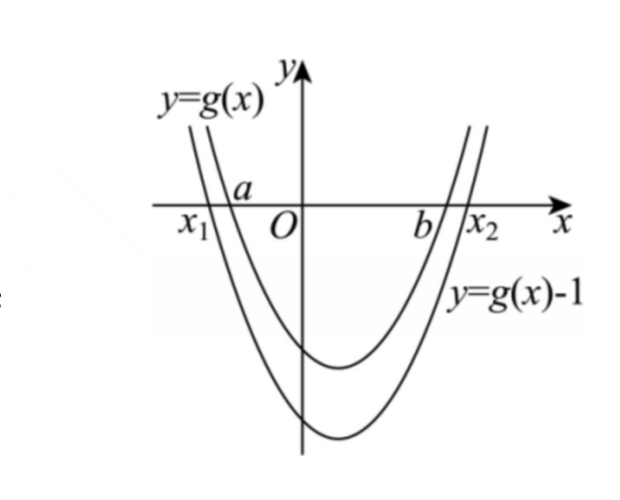
\includegraphics[width=0.20\textwidth]{figures/gao103_q16.png}
\end{center}
\step{由图像得 $x_1<a<b<x_2$．故选 $B$.}
\solend

\fi

\end{enumerate}

\bigsec{三、解答题}

\begin{enumerate}
\setcounter{enumi}{16}

\item 已知集合 $A=\{x\mid-3\leqslant x\leqslant1\}$，$B=\{x\mid a-2<x<a+2,a\in\R\}$.

（1）当 $a=1$ 时，求 $A\cap B$、$A\cup B$；

（2）若 $B\subseteq\overline A$，求 $a$ 的取值范围.

\ansspace*[8]

\ifanswer
\solbegin
\stepm{（1）}{当 $a=1$ 时，$B=\{x\mid-1<x<3\}$，又因为 $A=\{x\mid-3\leqslant x\leqslant1\}$，}
\step{所以 $A\cap B=\{x\mid-1<x\leqslant1\}$，$A\cup B=\{x\mid-3\leqslant x<3\}$；}
\stepm{（2）}{由 $A=\{x\mid-3\leqslant x\leqslant1\}$，得 $\overline A=\{x\mid x<-3\text{ 或 }x>1\}$，}
\step{若 $B\subseteq\overline A$，易得 $B=\{x\mid a-2<x<a+2,a\in\R\}\neq\varnothing$，}
\step{所以 $a+2\leqslant-3$ 或 $a-2\geqslant1$，解得 $a\leqslant-5$ 或 $a\geqslant3$，}
\step{综上所述，实数 $a$ 的取值范围是 $(-\infty,-5]\cup[3,+\infty)$.}
\solend

\fi

\item （1）解不等式 $\lvert 1-2x\rvert>x$；

（2）已知 $a$、$b$ 都是有理数，满足 $a+b\sqrt5=0$，请用反证法证明：$a=b=0$.

\ansspace*[10]

\ifanswer
\solbegin
\stepm{（1）}{①当 $x<0$ 时，左边非负，右边为负，不等式显然成立；}
\step{②当 $x\geqslant0$ 时，两边平方，$(1-2x)^2>x^2\Rightarrow3x^2-4x+1>0$}
\step{$\Rightarrow(3x-1)(x-1)>0$，解得 $x<\dfrac13$ 或 $x>1$，结合 $x\geqslant0$，}
\step{得 $0\leqslant x<\dfrac13$ 或 $x>1$；}
\step{综上，不等式解集为 $\left(-\infty,\dfrac13\right)\cup(1,+\infty)$.}
\stepm{（2）}{假设 $a,b$ 至少有一个不为零，}
\step{当 $a,b$ 中有一个为零一个不为零时，不妨设 $\begin{cases}a\neq0\\ b=0\end{cases}$，}
\step{则 $a+b\sqrt5=0\Rightarrow a=0$ 矛盾，舍；}
\step{当 $\begin{cases}a\neq0\\ b\neq0\end{cases}$ 时，$a+b\sqrt5=0\Rightarrow\sqrt5=-\dfrac ab\in\Q$，矛盾，舍，}
\step{综上假设不成立，所以 $a=b=0$.}
\solend

\fi

\item 某物流公司为了扩大业务量，计划建造一间高为 6 米，底面积为 24 平方米，且背面靠
墙的长方形形状的仓库。仓库的背面靠墙，无须建造费用，因此甲工程队给出的报价为：
仓库前面新建墙体每平方米 400 元，左右两面新建墙体每平方米 300 元，屋顶和地面以及
其他共计 28800 元.

（1）设仓库前面墙体的长为 $x$ 米 $(x>0)$，甲工程队的整体报价为 $y$ 元。若该物流公司计
划投入的改造资金不超过 60000 元，求前面墙体长 $x$ 的取值范围.

（2）在（1）的条件下，当仓库前面墙体的长度为多少时，甲工程队的整体
报价最低？

\begin{center}
% 原图第 7 页题干仓库示意图直接裁取（原卷排于题干右侧），已去粉色水印转灰度。
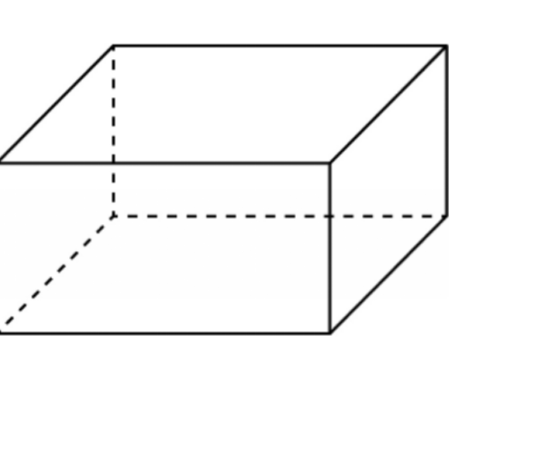
\includegraphics[width=0.17\textwidth]{figures/gao103_q19.png}
\end{center}

\ansspace*[12]

\ifanswer
\solbegin
\stepm{（1）}{甲队整体报价为 $y=400\times6x+2\times300\times6\times\dfrac{24}{x}+28800$}
\step{$=2400x+\dfrac{86400}{x}+28800$ 元，}
\step{要求 $y\leqslant60000$，即 $2400x+\dfrac{86400}{x}+28800\leqslant60000$，}
\step{化简得 $x+\dfrac{36}{x}\leqslant13$，}
\step{由于 $x>0$，则不等式化为 $x^2-13x+36\leqslant0$，}
\step{即 $(x-4)(x-9)\leqslant0$，解得 $4\leqslant x\leqslant9$，}
\step{所以前面墙体长 $x$ 的取值范围为 $[4,9]$；}
\stepm{（2）}{甲队整体报价为 $y=2400x+\dfrac{86400}{x}$}
\step{$\geqslant2\sqrt{2400x\times\dfrac{86400}{x}}+28800=57600$，}
\step{当且仅当 $2400x=\dfrac{86400}{x}$，即 $x^2=36$，}
\step{解得 $x=6$（满足 $4\leqslant x\leqslant9$）时取等号，}
\step{所以当仓库前面墙体的长度为 6 米时，甲工程队的整体报价最低，}
\step{为 57600 元.}
\solend

\fi

\item 已知函数 $f(x)=ax^2-10x+4b$.

（1）当 $a=1$，$b=4$ 时，解不等式 $f(x)\geqslant0$；

（2）若关于 $x$ 的不等式 $f(x)<0$ 的解集为 $(a,b)$，求实数 $a$、$b$ 的值；

（3）若 1 是 $f(x)$ 的零点，且 $a>0$，$b>0$，问当 $a$、$b$ 取何值时，$\dfrac1a+\dfrac1b$ 的值最小？最
小值是多少？

\ansspace*[12]

\ifanswer
\solbegin
\stepm{（1）}{将 $a=1$，$b=4$ 代入得 $f(x)=x^2-10x+16\geqslant0$，解得 $x\geqslant8$ 或 $x\leqslant2$，}
\step{所以不等式的解集为 $\{x\mid x\geqslant8\text{ 或 }x\leqslant2\}$；}
\stepm{（2）}{由题意得 $a$、$b$ 是 $ax^2-10x+4b=0$ 两根，且 $a<b$，$a>0$，}
\step{由韦达定理得 $\begin{cases}a+b=\dfrac{10}{a}\\ a\cdot b=\dfrac{4b}{a}\end{cases}$，解得 $\begin{cases}a=2\\ b=3\end{cases}$，即实数 $a$、$b$ 的值分别为 2，3；}
\stepm{（3）}{由 1 是 $f(x)$ 的零点，得 $f(1)=a-10+4b=0$，得 $a+4b=10$，}
\step{因为 $a>0$，$b>0$，}
\step{所以 $\dfrac1a+\dfrac1b=\dfrac1{10}\left(\dfrac1a+\dfrac1b\right)(a+4b)=\dfrac1{10}\left(1+4+\dfrac{4b}{a}+\dfrac ab\right)$}
\step{$\geqslant\dfrac1{10}\left(5+2\sqrt{\dfrac{4b}{a}\cdot\dfrac ab}\right)=\dfrac9{10}$，}
\step{当且仅当 $\dfrac{4b}{a}=\dfrac ab$，即 $a=\dfrac{10}3$,$b=\dfrac53$ 时取等号，}
\step{所以 $\dfrac1a+\dfrac1b$ 取最小值，且最小值为 $\dfrac9{10}$.}
\solend

\fi

\item 已知集合 $A$ 为非空集合，定义 $S=\{x\mid x=a+b,a,b\in A\}$，
$T=\{x\mid x=\lvert a-b\rvert,a,b\in A\}$.

（1）若集合 $A=\{1,3\}$，直接写出集合 $S$、$T$ (无需写计算过程)；

（2）若集合 $A=\{x_1,x_2,x_3,x_4\},x_1<x_2<x_3<x_4$，且 $T=A$，求证：$x_1+x_4=x_2+x_3$；

（3）若集合 $A=\{x\mid0\leqslant x\leqslant2026,x\in\N\}$,$S\cap T=\varnothing$．记 $\lvert A\rvert$ 为集合 $A$ 中元素的个数，求
$\lvert A\rvert$ 的最大值.

\ansspace*[16]

\ifanswer
\solbegin
\stepm{（1）}{$S=\{2,4,6\}$,$T=\{0,2\}$；}
\stepm{（2）}{集合 $T$ 中最小的元素为 0，因为 $T=A$，且 $x_1<x_2<x_3<x_4$，所以 $x_1=0$，}
\step{所以集合 $T$ 中元素为 $x_2-x_1=x_2$,$x_3-x_1=x_3$,$x_4-x_1=x_4$，}
\step{以及 $x_3-x_2$,$x_4-x_2$,$x_4-x_3$ 均属于 $A$，}
\step{因为 $x_1=0<x_3-x_2<x_4-x_2<x_4$，所以 $x_3$ 即 $x_4-x_2=x_3-x_1$，}
\step{即 $x_1+x_4=x_2+x_3$；}
\stepm{（3）}{设 $A=\{a_1,a_2,a_3,\cdots,a_k\}$ 满足题意，其中 $a_1<a_2<\cdots<a_k$，}
\step{则 $2a_1<a_1+a_2<\cdots<a_1+a_k<a_2+a_k<a_3+a_k<\cdots<a_{k-1}+a_k<2a_k$，}
\step{所以 $\lvert S\cup T\rvert\leqslant2k+1$，所以 $3k-1\leqslant2a_k+1\leqslant4053(k\in\N^*)$，}
\step{所以 $k\leqslant1351$，}
\step{实际上当 $A=\{676,677,\cdots,2026\}$ 时满足题意，}
\step{证明如下：设 $A=\{m,m+1,m+2,\cdots,2026\},m\in N$，}
\step{设 $S=\{2m,2m+1,2m+2,\cdots,4052\}$,$T=\{0,1,2,\cdots,2026-m\}$，}
\step{由题意得 $2026-m<2m$，即 $m>675\dfrac13$，}
\step{故 $m$ 的最小值是 676，于是当 $m=676$,$A$ 中的元素最多，}
\step{即 $A=\{676,677,\cdots,2026\}$ 时满足题意，}
\step{综上所述，集合 $A$ 中元素的个数的最大值是 1351.}
\solend

\fi

\end{enumerate}

\end{document}
